\documentclass[openany]{ctexbook}
\ctexset { chapter = { name={}, number={\arabic{chapter}} } }
\ctexset { section = { number={} } }
\ctexset { subsection = { number={} } }

\usepackage{fontspec}
\setmainfont{Linux Libertine O}
\setsansfont{Droid Sans}
\setmonofont{CMU Typewriter Text}

% \usepackage{geometry}
\usepackage[showframe]{geometry}
\geometry{left=2.54cm, right=2.54cm, top=3.18cm, bottom=3.18cm}

% 应在 geometry 之后引入 不然页眉线不撑满整个宽度
\usepackage{fancyhdr}
\pagestyle{fancy}
\fancyhf{}
\fancyhead[LO]{\color{red}\nouppercase\rightmark}
\fancyhead[LE,RO]{\color{red}\thepage}
\fancyhead[RE]{\color{red}\nouppercase\leftmark}
\renewcommand{\headrulewidth}{0.6pt}
\renewcommand{\chaptermark}[1]{\markboth{\thechapter:#1}{}}
\renewcommand{\sectionmark}[1]{\markright{#1}}
\setlength{\headheight}{12.64723pt}
\addtolength{\topmargin}{-0.64723pt}

\usepackage{indentfirst}

\usepackage{titlesec}
\titleformat{\chapter}{\color{red}\LARGE\bfseries\centering}{\thechapter :}{.5em}{}[\vspace*{1em}\titlerule]
\titleformat{\section}{\color{red}\Large\bfseries}{}{0pt}{}
\titleformat{\subsection}{\color{red}\large\bfseries}{}{0pt}{}

\usepackage{titletoc}
\titlecontents{section}[2em]{\addvspace{2pt}\filright}{}{}{\titlerule*[8pt]{.}\contentspage}
\titlecontents{subsection}[4em]{\addvspace{2pt}\filright}{}{}{\titlerule*[8pt]{.}\contentspage}

\usepackage{xpatch}
\xpretocmd\headrule{\color{red}}{}{\PatchFailed}

\usepackage{xurl}
% make te text hyphenat
\usepackage[htt]{hyphenat}
\usepackage{xcolor}
\definecolor{lightgray}{rgb}{.9, .9, .9}

\usepackage{enumitem}
\setlist[itemize]{font=\ttfamily, itemsep=0pt, parsep=0pt}
% \setlist{nolistsep}

\usepackage{float}
\usepackage{caption}
\captionsetup{
  font={large, bf},
  labelfont={small, color=red},
  % labelsep=quad,
  justification=centering,
}

\usepackage{tikz}
\usepackage{graphicx}
\usepackage[all,pdf,color]{xy}
\usepackage{rotating}
\usepackage{float}

\usepackage{makeidx}
\makeindex

\usepackage{hyperref}
\hypersetup{
  bookmarksnumbered,
  colorlinks
}

\usepackage[framemethod=TikZ]{mdframed}
\mdfsetup{
  linecolor=purple!50!black,
  backgroundcolor=lightgray,
  shadow,
  innertopmargin=0pt,
  innerbottommargin=0pt,
  innerleftmargin=2pt,
}

\usepackage[cachedir=../_minted-main]{minted}
% xleftmargin=20pt
\setminted[typescript]{
  fontsize=\small,
  breaklines,
  linenos,
  escapeinside=\%\%,
  % 使用 mdframed 代替
  % bgcolor=lightgray,
  % frame=single,
  % rulecolor=purple!50!black,
}
\usemintedstyle{perldoc}
\renewcommand{\theFancyVerbLine}{\ttfamily
  \textcolor[rgb]{0.5,0.5,1.0}{\small
    \oldstylenums{\arabic{FancyVerbLine}}}}

% https://tex.stackexchange.com/questions/228058/how-to-space-before-and-after-a-minted-code-block-with-bgcolor
\usepackage{etoolbox}
\makeatletter
\patchcmd{\minted@colorbg}{\noindent}{\vspace{0pt}\noindent}{}{}
\apptocmd{\endminted@colorbg}{\par\vspace{0pt}}{}{}
\makeatother

% \BeforeBeginEnvironment{minted}{\begin{mdframed}}
% \AfterEndEnvironment{minted}{\end{mdframed}}
\surroundwithmdframed{minted}
\newcommand\step[1]{\setlength\fboxsep{1.5pt}\colorbox{black}{\textcolor{white}{#1}}}
\newcommand\ts[1]{\mintinline{ts}{#1}}
\newcommand\fref[1]{见图 \ref{#1}}

\makeindex
\begin{document}
\title{Clipcode{\texttrademark} Source Tour For Angular 12 \footnote{ecuplxd 翻译,仅供参考。版本:2021-05-08}
  \\[1ex] \large A detailed guided tour to the source trees of Angular and related projects
}
\author{
  \\[32ex]
  \emph{Copyright (c) 2021 Clipcode Limited - All rights reserved} \\
  \emph{Clipcode is a trademark of Clipcode Limited - All rights reserved}
}
\date{}
\frontmatter
\maketitle
\setcounter{tocdepth}{3}
\tableofcontents
\chapter{Preface}

% Mainly C++ (with some C and x86/ARM hand-coded assembly)
% written in
% tslint
% ng-packagr
% NgRx

% Note JAVA is used by Bazel build system to build Angular itself – it is not needed at all
% when building your own Angular applications (unless you use Bazel, a good option for
% very large code bases). Note moment.js is a very popular date and time framework.
% We see it used by the
% \url{@angular/material-moment-adapter}
% package.
% Angular Main Project System Model

% (number in box is size of /src sub-directory)

\section{An Ecosystem for Modern Web Applications}

The Angular ecosystem consists of multiple projects that work together to provide a
comprehensive foundation for developing modern web applications.  With a few
exceptions, all of these projects are written with TypeScript (even the TypeScript
compiler is itself written in TypeScript). The exceptions are the Bazel main project
(which uses Java), fsevents for native access to macOS FSEvents along with the
Jasmine unit test framework and Karma test runner (all these use JavaScript). The
dependency on other projects varies.

Note that the Java-based Bazel main project is used to build Angular itself. Bazel and
Java are not needed to build regular Angular applications. Bazel is great for
incremental and multi-core builds so it has advantages when used with large
codebases (such as Angular itself). In future Bazel is likely to become a sensible build
option for larger Angular applications.

None of these projects are dependent on Visual Studio Code. These projects only need
a code editor that can work with the TypeScript tsc compiler – and there are many -
see middle of main page at:

\begin{itemize}
  \item \url{http://typescriptlang.org}
\end{itemize}

Visual Studio Code is one such editor, that is particularly good, open source, freely
available for macOS, Linux and Windows, and it too is written in TypeScript.

\begin{itemize}
  \item \url{https://code.visualstudio.com}
\end{itemize}

Of choose you can use any editor to investigate the source trees of these projects.

\subsection{Viewing Markdown Files}

% In addition to source in TypeScript, all these projects also contain documentation files
% in markdown format (*.md). Markdown is a domain specific language (DSL) for
% represent HTML documents. It is easier / quicker to manually author compared to
% HTML. When transformed to HTML it provides professional documentation. One
% question you might have is how to view them (as HTML, rather that as .md text). One
% easy way to see them as html is just to view the .md files on Github, e.g.:

\begin{itemize}
  \item \url{https://github.com/angular/angular}
\end{itemize}

% Alternatively, on your own machine, most text editors have either direct markdown
% support or it is available through extensions. When examining a source tree with .md
% files, it is often useful when your code editor can also open markdown files and
% transform them to HTML when requested. StackOverflow covers this issue here:

\begin{itemize}
  \item \url{http://stackoverflow.com/questions/9843609/view-markdown-files-offline}
\end{itemize}

% For example, Visual Studio Code supports Markdown natively and if you open a .md
% file and select CTRL+SHIFT+V, you get to see nice HTML:

\begin{itemize}
  \item \url{https://code.visualstudio.com/docs/languages/markdown}
\end{itemize}

% Finally, if you want to learn markdown, try here:

\begin{itemize}
  \item \url{http://www.markdowntutorial.com}
\end{itemize}


\section{Target Audience}

% This guided tour of the Angular source tree is aimed at intermediate to advanced
% application developers who wish to develop a deeper understanding of how Angular
% actually works. To really appreciate the functioning of Angular, an application
% developer should read the source. Yes, Angular come with developer documentation
% at
% \url{https://angular.io/docs}
% (which is mostly quite good) but it is best studied in
% conjunction with the source code.

% \section{Benefits of Understanding The Source}
\section{理解源码的好处}

% There are many good reasons for intermediate- to advanced-developers to become
% familiar with the source trees of the projects that provide the foundation for their daily
% application development.

中高级开发人员有很多充分的理由需要熟悉 Angular 的源码,
因为他们日常的应用开发都需要和 Angular 打交道。

% Enhanced Understanding - As in common with many software packages, descriptions
% of software concepts and API documentation may or may not be present, and if
% present may not be as comprehensive as required, and what is present may or may
% not accurately reflect what the code currently does - the doc for a particular concept
% may well once have been up-to-date, but code changes, the doc not necessarily so,
% and certainly not in lock-step, and this applies to any fast evolving framework.

增强理解 —— 与许多软件包一样,
关于概念设计和 API 的文档可能存在也可能不存在,
如果存在也可能没有要求的那么全面,或多或少不能准确反映当前代码的真实意图 —— 文档过时了,
毕竟代码改动后,并不总是同步地更新文档,这适用于任何快速发展的框架。

% Advanced Debugging – When things go wrong, as they must assuredly will (and
% usually just become an important presentation to potential customers), application
% developers scrambling to fix problems will be much quicker when they have better
% insight via knowing the source.

高级调试 —— 当出现问题时,
因为它们肯定会出现(并且通常只是向潜在客户展示的一个重要展示),
如果深入了解过源码,能更快地解决问题。

% Optimization – for large-scale production applications with high data throughput,
% knowing how your application’s substrate actually works can be really useful in
% deciding how / what to optimize (for example, when application developers really
% understand how Angular’s
% \texttt{NgZone}
% works, how it is optional (from Angular v5 onwards)
% and how it is intertwined with Angular’s change detection, then they can place CPU-
% intensive but non-UI code in a different zone within the same thread, and this can
% result in much better performance).

优化 —— 对于具有高数据吞吐量的大规模生产应用,
了解应用的基板实际如何工作对于决定如何/优化什么非常有用
(例如,当应用开发人员真正了解 Angular 的 \texttt{NgZone} 的工作原理时,
它是如何可选的(从 Angular v5 开始)以及它如何与 Angular 的变更检测交织在一起,
然后他们可以将 CPU 密集型但非 UI 代码放置在同一线程内的不同区域中,
这可以带来更好的性能)。

% Productivity - Familiarity with the source is important for maximum productivity with
% any framework and is one part of a developer accumulating a broader understanding
% of the substrate upon which their applications execute.

生产力 —— 熟悉源码对于任何框架最大化生产力都是重要的,
是开发人员积累更广泛的理解的一部分以及应用如何执行的基础。

% Good practices – Studying large codebases that are well tested and subjected to
% detailed code reviews is a great way for “regular” developers to pick up good coding
% habits and use in their own application source trees.

良好实践 —— 研究经过良好测试和详细 review 的大型代码库
可以让开发人员养成良好编码习惯,并在自己的应用中实际运用。
\section{Accessing the Source}

% To study the source, you can browse it online, get a copy of the repo via git (usual) or
% download a zip. Some packages may provide extra detail about getting the source –
% for example, for the Angular project, read “Getting the Sources” here:

\begin{itemize}
  \item \url{https://github.com/angular/angular/blob/master/docs/DEVELOPER.md}
\end{itemize}

% We first need to decide which branch to use. For master, we use this:

\begin{itemize}
  \item \url{https://github.com/angular/angular/tree/master}
\end{itemize}

% Specifically for the Angular main project, an additional way to access the source is in
% the Angular API Reference (
% \url{https://angular.io/api}
% ), the API page for each Angular
% type has a hyperlink at the top of the page to the relevant source file (this resolves to
% the latest stable version, which may or may not be the same source as master).

\section{Keeping up to date}

% Angular is a fast evolving project. To keep up to date,  read the development team’s
% weekly meeting notes, which are available here:

\begin{itemize}
  \item \url{http://g.co/ng/weekly-notes}
\end{itemize}

% The Changelog in Github lists features of new releases:

\begin{itemize}
  \item \url{https://github.com/angular/angular/blob/master/CHANGELOG.md}
\end{itemize}


\section{An Ecosystem for Modern Web Applications}

The Angular ecosystem consists of multiple projects that work together to provide a
comprehensive foundation for developing modern web applications.  With a few
exceptions, all of these projects are written with TypeScript (even the TypeScript
compiler is itself written in TypeScript). The exceptions are the Bazel main project
(which uses Java), fsevents for native access to macOS FSEvents along with the
Jasmine unit test framework and Karma test runner (all these use JavaScript). The
dependency on other projects varies.

Note that the Java-based Bazel main project is used to build Angular itself. Bazel and
Java are not needed to build regular Angular applications. Bazel is great for
incremental and multi-core builds so it has advantages when used with large
codebases (such as Angular itself). In future Bazel is likely to become a sensible build
option for larger Angular applications.

None of these projects are dependent on Visual Studio Code. These projects only need
a code editor that can work with the TypeScript tsc compiler – and there are many -
see middle of main page at:

\begin{itemize}
  \item \url{http://typescriptlang.org}
\end{itemize}

Visual Studio Code is one such editor, that is particularly good, open source, freely
available for macOS, Linux and Windows, and it too is written in TypeScript.

\begin{itemize}
  \item \url{https://code.visualstudio.com}
\end{itemize}

Of choose you can use any editor to investigate the source trees of these projects.

\subsection{Viewing Markdown Files}

% In addition to source in TypeScript, all these projects also contain documentation files
% in markdown format (*.md). Markdown is a domain specific language (DSL) for
% represent HTML documents. It is easier / quicker to manually author compared to
% HTML. When transformed to HTML it provides professional documentation. One
% question you might have is how to view them (as HTML, rather that as .md text). One
% easy way to see them as html is just to view the .md files on Github, e.g.:

\begin{itemize}
  \item \url{https://github.com/angular/angular}
\end{itemize}

% Alternatively, on your own machine, most text editors have either direct markdown
% support or it is available through extensions. When examining a source tree with .md
% files, it is often useful when your code editor can also open markdown files and
% transform them to HTML when requested. StackOverflow covers this issue here:

\begin{itemize}
  \item \url{http://stackoverflow.com/questions/9843609/view-markdown-files-offline}
\end{itemize}

% For example, Visual Studio Code supports Markdown natively and if you open a .md
% file and select CTRL+SHIFT+V, you get to see nice HTML:

\begin{itemize}
  \item \url{https://code.visualstudio.com/docs/languages/markdown}
\end{itemize}

% Finally, if you want to learn markdown, try here:

\begin{itemize}
  \item \url{http://www.markdowntutorial.com}
\end{itemize}


\section{Target Audience}

% This guided tour of the Angular source tree is aimed at intermediate to advanced
% application developers who wish to develop a deeper understanding of how Angular
% actually works. To really appreciate the functioning of Angular, an application
% developer should read the source. Yes, Angular come with developer documentation
% at
% \url{https://angular.io/docs}
% (which is mostly quite good) but it is best studied in
% conjunction with the source code.

% \section{Benefits of Understanding The Source}
\section{理解源码的好处}

% There are many good reasons for intermediate- to advanced-developers to become
% familiar with the source trees of the projects that provide the foundation for their daily
% application development.

中高级开发人员有很多充分的理由需要熟悉 Angular 的源码,
因为他们日常的应用开发都需要和 Angular 打交道。

% Enhanced Understanding - As in common with many software packages, descriptions
% of software concepts and API documentation may or may not be present, and if
% present may not be as comprehensive as required, and what is present may or may
% not accurately reflect what the code currently does - the doc for a particular concept
% may well once have been up-to-date, but code changes, the doc not necessarily so,
% and certainly not in lock-step, and this applies to any fast evolving framework.

增强理解 —— 与许多软件包一样,
关于概念设计和 API 的文档可能存在也可能不存在,
如果存在也可能没有要求的那么全面,或多或少不能准确反映当前代码的真实意图 —— 文档过时了,
毕竟代码改动后,并不总是同步地更新文档,这适用于任何快速发展的框架。

% Advanced Debugging – When things go wrong, as they must assuredly will (and
% usually just become an important presentation to potential customers), application
% developers scrambling to fix problems will be much quicker when they have better
% insight via knowing the source.

高级调试 —— 当出现问题时,
因为它们肯定会出现(并且通常只是向潜在客户展示的一个重要展示),
如果深入了解过源码,能更快地解决问题。

% Optimization – for large-scale production applications with high data throughput,
% knowing how your application’s substrate actually works can be really useful in
% deciding how / what to optimize (for example, when application developers really
% understand how Angular’s
% \texttt{NgZone}
% works, how it is optional (from Angular v5 onwards)
% and how it is intertwined with Angular’s change detection, then they can place CPU-
% intensive but non-UI code in a different zone within the same thread, and this can
% result in much better performance).

优化 —— 对于具有高数据吞吐量的大规模生产应用,
了解应用的基板实际如何工作对于决定如何/优化什么非常有用
(例如,当应用开发人员真正了解 Angular 的 \texttt{NgZone} 的工作原理时,
它是如何可选的(从 Angular v5 开始)以及它如何与 Angular 的变更检测交织在一起,
然后他们可以将 CPU 密集型但非 UI 代码放置在同一线程内的不同区域中,
这可以带来更好的性能)。

% Productivity - Familiarity with the source is important for maximum productivity with
% any framework and is one part of a developer accumulating a broader understanding
% of the substrate upon which their applications execute.

生产力 —— 熟悉源码对于任何框架最大化生产力都是重要的,
是开发人员积累更广泛的理解的一部分以及应用如何执行的基础。

% Good practices – Studying large codebases that are well tested and subjected to
% detailed code reviews is a great way for “regular” developers to pick up good coding
% habits and use in their own application source trees.

良好实践 —— 研究经过良好测试和详细 review 的大型代码库
可以让开发人员养成良好编码习惯,并在自己的应用中实际运用。
\section{Accessing the Source}

% To study the source, you can browse it online, get a copy of the repo via git (usual) or
% download a zip. Some packages may provide extra detail about getting the source –
% for example, for the Angular project, read “Getting the Sources” here:

\begin{itemize}
  \item \url{https://github.com/angular/angular/blob/master/docs/DEVELOPER.md}
\end{itemize}

% We first need to decide which branch to use. For master, we use this:

\begin{itemize}
  \item \url{https://github.com/angular/angular/tree/master}
\end{itemize}

% Specifically for the Angular main project, an additional way to access the source is in
% the Angular API Reference (
% \url{https://angular.io/api}
% ), the API page for each Angular
% type has a hyperlink at the top of the page to the relevant source file (this resolves to
% the latest stable version, which may or may not be the same source as master).

\section{Keeping up to date}

% Angular is a fast evolving project. To keep up to date,  read the development team’s
% weekly meeting notes, which are available here:

\begin{itemize}
  \item \url{http://g.co/ng/weekly-notes}
\end{itemize}

% The Changelog in Github lists features of new releases:

\begin{itemize}
  \item \url{https://github.com/angular/angular/blob/master/CHANGELOG.md}
\end{itemize}


\mainmatter
\chapter{Internals Of Zone.js}

% \emph{This document explores the internals of the Zone.js library and how it is}
% \emph{used from within a sample large framework, Angular 12.}

% \section{Overview}
\section{概览}

% The Zone.js project provides multiple asynchronous execution contexts running within
% a single JavaScript thread (i.e. within the main browser UI thread or within a single
% web worker). Zones are a way of sub-dividing a single thread using the JavaScript
% event loop. A single zone does not cross thread boundaries. A nice way to think about
% zones is that they sub-divide the stack within a JavaScript thread into multiple mini-
% stacks, and sub-divide the JavaScript event loop into multiple mini event loops that
% seemingly run concurrently (but really share the same VM event loop). In effect,
% Zone.js helps you write multithreaded code within a single thread.

Zone.js 项目提供了在单个 JavaScript 线程中运行多个异步执行上下文
(即主浏览器 UI 线程或单个 web worker 中)。
Zone 使用了将 JavaScript 事件循环分割单个线程的方式。
单个 zone 不会跨越线程边界。
考虑 zone 的良好方法是它们将 JavaScript 线程内的栈分割成多个小栈,
并将 JavaScript 事件循环分划分为多个小的事件循环,
这些循环似乎同时运行(但却共享相同的 VM 事件循环)。
实际上,Zone.js 有助于你在单线程中编写多线程代码。

% When Zone.js is loaded by your app, it monkey-patches certain asynchronous calls
% (e.g.
% \texttt{setTimer}
% ,
% \texttt{addEventListener}
% ) to implement zone functionality. Zone.js does
% this by adding wrappers to the callbacks the application supplies, and when a timeout
% occurs or an event is detected, it runs the wrapper first and then the application
% callback. Chunks of executing application code form tasks and each task executes in
% the context of a zone. Zones are arranged in a hierarchy and provide useful features
% in areas such as error handling, performance measuring and executing configured
% work items upon entering and leaving a zone (all of which might be of great interest
% to implementors of change detection in a modern web UI framework, like Angular).

当你的应用程序加载 Zone.js 时,
它会修补某些异步调用(例如 \texttt{setTimer}、\texttt{addEventListener})来实现 zone 功能。
Zone.js 通过向应用提供的回调函数添加包装器做到这点,
当超时或检测到事件时,它首先运行包装器,然后运行回调。
执行应用程序代码形成任务的块,每个任务在 zone 的上下文。
Zones 按层次排列并提供有用的功能在错误处理、性能测量和执行配置等领域进入和离开 zone 时的工作项目
(所有这些对自己实现现代 Web UI 框架中变更检测有参考价值)。

% Zone.js is mostly transparent to application code. Zone.js runs in the background and
% for the most part “just works”. For example, Angular uses Zone.js and Angular
% application code usually runs inside a zone. Tens of thousands of Angular application
% developers have their code execute within zones without evening knowing these exist.
% More advanced applications can have custom code to make zone API calls if needed
% and become more actively involved in zone management. Some application
% developers may wish to take certain steps to move some non-UI performance-critical
% code outside of the Angular zone – using the
% \href{https://next.angular.io/api/core/NgZone}{NgZone}
% class).

Zone.js 对应用代码大多是透明的。Zone.js 在后台运行,大部分“只是默默工作”。
例如,Angular 使用 Zone.js,Angular 应用代码通常运行在 zone 内。
成千上万的 Angular 应用开发人员甚至都没意识到这点。
如果有需要,可以自定义 zone API 调用,手动管理 zone 的运行。
有些应用开发人员可能希望采取某些步骤将非 UI 性能关键代码移出 Angular zone ——
这时可以使用 \href{https://next.angular.io/api/core/NgZone}{NgZone} 类。

\subsection{Project Information}

% The homepage + root of the source tree for Zone.js are in the main Angular repo at:

\begin{itemize}
  \item \url{https://github.com/angular/angular/tree/master/packages/zone.js}
\end{itemize}

% Below we assume you have got the Zone.js source tree downloaded locally under a
% directory we will call <ZONE-MASTER> and any pathnames we use will be relative to
% that. We also will look at the Angular code that calls Zone.js and we use the
% <ANGULAR-MASTER> as the root of that source tree.

% Zone.js is written in TypeScript. It has no package dependencies (its package.json has
% this entry:
% \texttt{"dependencies": {}}
% ), though it has many
% \texttt{devDependencies}
% . It is quite a
% small source tree, whose size (uncompressed) is about 3 MB.


\section{Using Zone.js}

Before looking in detail at how Zone.js itself is implemented, we will first look at how
it is used in production, using the example of the very popular Angular project.

The use of Zone.js with Angular is optional, but used by default. Use of zones is
mostly a good idea but there are some scenarios (e.g. using Angular Elements to build
Web Compoenents) when this is not the case.

To use Zone.js in your applications, you need to load it. Your package.json file will
need (if creating a project using Angular CLI, this is added automatically for you):

\begin{minted}{json}
  "dependencies": {
    ..,
    "zone.js": "<version>"
  },
\end{minted}


You should load Zone.js after loading core.js (if using that). For example, if using an
Angular application generated via Angular CLI (as most production apps will be),
Angular CLI will generate a file called <project-name>/src/polyfills.ts and it will
contain:

\begin{minted}{typescript}
/**************************************************************************
 * Zone JS is required by default for Angular itself.
 */
import 'zone.js/dist/zone'; // Included with Angular CLI.
\end{minted}


Angular CLI also generates an angular.json configuration file, with this line that sets
up polyfills:

\begin{minted}{ts}
 "build": {
          "builder": "@angular-devkit/build-angular:browser",
          "options": {
            ..
            "polyfills": "src/polyfills.ts",
\end{minted}


If writing your application in TypeScript (recommended), you also need to get access
to the ambient declarations. These define the Zone.js API and are supplied in:

\begin{itemize}
  \item \href{https://github.com/angular/zone.js/blob/master/dist/zone.js.d.ts}
        {<ZONE-MASTER>/dist/zone.js.d.ts}
\end{itemize}

(IMPORTANT: This file is particularly well documented and well worth some careful
study by those learning Zone.js). Unlike declarations for most other libraries,
zone.js.d.ts does not use
\texttt{import}
or
\texttt{export}
at all (those constructs do not appear
even once in that file). That means application code wishing to use zones cannot
simply import its .d.ts file, as is normally the case. Instead, the
\texttt{///reference}
construct needs to be used. This includes the referenced file at the site of the
\texttt{///reference}
in the containing file. The benefit of this approach is that the containing
file itself does not have to (but may) use
\texttt{import}
, and thus may be a script, rather
than having to be a module. The use of zones is not forcing the application to use
modules (however, most larger applications, including all Angular applications - will).
How this works is best examined with an example, so lets look at how Angular
includes zone.d.ts. Angular contains a file, types.d.ts under its packages directory
(and a similar one under its modules directory and tools directory):

\begin{itemize}
  \item \href{https://github.com/angular/angular/blob/master/modules/types.d.ts}
        {<ANGULAR-MASTER>/packages/types.d.ts}
\end{itemize}

and it has the following contents:

\begin{minted}{typescript}
/// <reference types="hammerjs" />
/// <reference types="jasmine" />
/// <reference types="jasminewd2" />
/// <reference types="node" />
/// <reference types="zone.js" />
/// <reference lib="es2015" />
/// <reference path="./system.d.ts" />
\end{minted}


% \subsection{Use Within Angular}
\subsection{在 Angular 中使用}

% When writing Angular applications, all your application code runs within a zone, unless
% you take specific steps to ensure some of it does not. Also, most of the Angular
% framework code itself runs in a zone. When beginning Angular application
% development, you can get by simply ignoring zones, since they are set up correctly by
% default for you and applications do not have to do anything in particular to take
% advantage of them. The end of the file
% \href{https://github.com/angular/zone.js/blob/master/MODULE.md}
% {<ZONE-MASTER>/blob/master/MODULE.md}
% explains where Angular uses zones:

编写 Angular 应用时,你的所有应用代码都在一个 zone 内运行,
除非你采取具体步骤以确保其中一些不会。
此外,大多数 Angular 框架代码本身在一个 zone 中运行。
开始 Angular 应用时开发,你可以简单地忽略 zones,
它们默认为你的应用配置好了,无需做任何特别的事情就能从中受益。
文件
\href{https://github.com/angular/zone.js/blob/master/MODULE.md}
{<ZONE-MASTER>/blob/master/MODULE.md} 文件结尾
结尾解释了 Angular 在哪里使用到了 zones:

\emph{“Angular uses zone.js to manage async operations and decide when to perform}
\emph{change detection. Thus, in Angular, the following APIs should be patched, otherwise}
\emph{Angular may not work as expected.}

\begin{itemize}
  \item ZoneAwarePromise
  \item timer
  \item on\_property
  \item EventTarget
  \item XHR”
\end{itemize}

% Zones are how Angular initiates change detection – when the zone’s mini-stack is
% empty, change detection occurs. Also, zones are how Angular configures global
% exception handlers. When an error occurs in a task, its zone’s configured error handler
% is called. A default implementation is provided and applications can supply a custom
% implementation via dependency injection. For details, see here:

Zones 是 Angular 启动变更检测的方式 —— 当 zone 的小块栈是空时,发生变更检测。
此外,zones 是 Angular 配置全局异常处理的方式。
当任务发生错误时,其 zone 配置的错误处理程序被调用。
Zone 提供了默认实现,应用可以通过依赖注入提供自定义实现。
有关详细信息,请参见此处:

\begin{itemize}
  \item \url{https://angular.io/api/core/ErrorHandler}
\end{itemize}

% On that page note the code sample about setting up your own error handler:

在该页面上,提供了自定义错误处理程序的代码示例:

\input{../output/1_internals_of_zone_js/code/1_1_0_0.tex}

% Angular provide a class,
% \texttt{NgZone}
% , which builds on zones:

Angular 提供了一个类 \texttt{NgZone},它建立在 zone 上:

\begin{itemize}
  \item \url{https://angular.io/api/core/NgZone}
\end{itemize}

% As you begin to create more advanced Angular applications, specifically those
% involving computationally intensive code that does not change the UI midway through
% the computation (but may at the end), you will see it is desirable to place such CPU-
% intensive work in a separate zone, and you would use a custom
% \texttt{NgZone}
% for that.

当你开始创建更高级的 Angular 应用程序时,
特别是那些涉及不会在中途更改 UI 的计算密集型代码计算(但可能在最后),
您会看到放置这样的 CPU 是可取的-
在单独的区域中进行密集的工作,您将为此使用自定义 \texttt{NgZone}。

% Elsewhere we will be looking in detail at
% \texttt{NgZone}
% and the use of zones within Angular in
% general when we explore the source tree for the main Angular project later, but for
% now, note the source for
% \texttt{NgZone}
% is in:

在其他地方,
我们将详细介绍 \texttt{NgZone} 和 Angular 中 zones 的使用一般当我们稍后探索主要 Angular 项目的源码时,
但对于现在,请注意 \texttt{NgZone} 的源码在:

\begin{itemize}
  \item \href{https://github.com/angular/angular/tree/master/packages/core/src/zone}
        {<ANGULAR-MASTER>/packages/core/src/zone}
\end{itemize}

% and the zone setup during bootstrap for an application is in:

应用程序引导期间的 zone 设置位于:

\begin{itemize}
  \item \href{https://github.com/angular/angular/blob/master/packages/core/src/application_ref.ts}
        {<ANGULAR-MASTER>/packages/core/src/application\_ref.ts}
\end{itemize}

% When we bootstrap our Angular applications, we either use
% \texttt{bootstrapModule<M>}
% (using the dynamic compiler) or
% \texttt{bootstrapModuleFactory<M>}
% (using the offline
% compiler). Both these functions are in application\_ref.ts.
% \texttt{bootstrapModule<M>}
% calls
% the Angular compiler
% 1
% and then calls
% \texttt{bootstrapModuleFactory<M>}
% \texttt{2}
% \texttt{.}


当我们引导 Angular 应用程序时,我们要么使用 \texttt{bootstrapModule<M>}
(使用动态编译器)或 \texttt{bootstrapModuleFactory<M>}(使用离线编译器)。
这两个函数都在 application\_ref.ts. \texttt{bootstrapModule<M>}
调用 Angular 编译器 \step{1} 然后调用 \texttt{bootstrapModuleFactory<M>} \step{2}。

\input{../output/1_internals_of_zone_js/code/1_1_0_1.tex}

% It is in
% \texttt{bootstrapModuleFactory}
% we see how zones are initialized for Angular:

在 \texttt{bootstrapModuleFactory} 中,我们看到了如何为 Angular 初始化 zone:

\input{../output/1_internals_of_zone_js/code/1_1_0_2.tex}

% At
% 1
% we see a new
% \texttt{NgZone}
% being created and at
% 2
% its
% \texttt{run()}
% method being called, at
% 3
% we see an error handler implementation being requested from dependency injection (a
% default implementation will be returned unless the application supplies a custom one)
% and at
% 4
% , we see that error handler being used to configure error handling for the
% newly created
% \texttt{NgZone}
% . Finally at
% 5
% , we see the call to the actual bootstrapping.

在 \step{1} 我们看到一个新的 \texttt{NgZone} 被创建,
在 \step{2} 它的 \texttt{run()} 方法被调用,
在 \step{3} 我们看到依赖注入请求了一个错误处理实现
(除非应用提供自定义实现,否则将返回默认实现)
在 \step{4} 处,我们看到错误处理程序将被用于配置新创建的 \texttt{NgZone}。
最后在 \step{5} 处,我们看到对实际引导的调用。

% So in summary, Angular application developers should clearly learn about zones, since
% that is the execution context within which their application code will run.

所以总而言之,Angular 应用开发人员应该清楚地了解 zones,
因为他们的应用代码将在其中的执行上下文运行。


% \subsection{Use Within Angular}
\subsection{在 Angular 中使用}

% When writing Angular applications, all your application code runs within a zone, unless
% you take specific steps to ensure some of it does not. Also, most of the Angular
% framework code itself runs in a zone. When beginning Angular application
% development, you can get by simply ignoring zones, since they are set up correctly by
% default for you and applications do not have to do anything in particular to take
% advantage of them. The end of the file
% \href{https://github.com/angular/zone.js/blob/master/MODULE.md}
% {<ZONE-MASTER>/blob/master/MODULE.md}
% explains where Angular uses zones:

编写 Angular 应用时,你的所有应用代码都在一个 zone 内运行,
除非你采取具体步骤以确保其中一些不会。
此外,大多数 Angular 框架代码本身在一个 zone 中运行。
开始 Angular 应用时开发,你可以简单地忽略 zones,
它们默认为你的应用配置好了,无需做任何特别的事情就能从中受益。
文件
\href{https://github.com/angular/zone.js/blob/master/MODULE.md}
{<ZONE-MASTER>/blob/master/MODULE.md} 文件结尾
结尾解释了 Angular 在哪里使用到了 zones:

\emph{“Angular uses zone.js to manage async operations and decide when to perform}
\emph{change detection. Thus, in Angular, the following APIs should be patched, otherwise}
\emph{Angular may not work as expected.}

\begin{itemize}
  \item ZoneAwarePromise
  \item timer
  \item on\_property
  \item EventTarget
  \item XHR”
\end{itemize}

% Zones are how Angular initiates change detection – when the zone’s mini-stack is
% empty, change detection occurs. Also, zones are how Angular configures global
% exception handlers. When an error occurs in a task, its zone’s configured error handler
% is called. A default implementation is provided and applications can supply a custom
% implementation via dependency injection. For details, see here:

Zones 是 Angular 启动变更检测的方式 —— 当 zone 的小块栈是空时,发生变更检测。
此外,zones 是 Angular 配置全局异常处理的方式。
当任务发生错误时,其 zone 配置的错误处理程序被调用。
Zone 提供了默认实现,应用可以通过依赖注入提供自定义实现。
有关详细信息,请参见此处:

\begin{itemize}
  \item \url{https://angular.io/api/core/ErrorHandler}
\end{itemize}

% On that page note the code sample about setting up your own error handler:

在该页面上,提供了自定义错误处理程序的代码示例:

\input{../output/1_internals_of_zone_js/code/1_1_0_0.tex}

% Angular provide a class,
% \texttt{NgZone}
% , which builds on zones:

Angular 提供了一个类 \texttt{NgZone},它建立在 zone 上:

\begin{itemize}
  \item \url{https://angular.io/api/core/NgZone}
\end{itemize}

% As you begin to create more advanced Angular applications, specifically those
% involving computationally intensive code that does not change the UI midway through
% the computation (but may at the end), you will see it is desirable to place such CPU-
% intensive work in a separate zone, and you would use a custom
% \texttt{NgZone}
% for that.

当你开始创建更高级的 Angular 应用程序时,
特别是那些涉及不会在中途更改 UI 的计算密集型代码计算(但可能在最后),
您会看到放置这样的 CPU 是可取的-
在单独的区域中进行密集的工作,您将为此使用自定义 \texttt{NgZone}。

% Elsewhere we will be looking in detail at
% \texttt{NgZone}
% and the use of zones within Angular in
% general when we explore the source tree for the main Angular project later, but for
% now, note the source for
% \texttt{NgZone}
% is in:

在其他地方,
我们将详细介绍 \texttt{NgZone} 和 Angular 中 zones 的使用一般当我们稍后探索主要 Angular 项目的源码时,
但对于现在,请注意 \texttt{NgZone} 的源码在:

\begin{itemize}
  \item \href{https://github.com/angular/angular/tree/master/packages/core/src/zone}
        {<ANGULAR-MASTER>/packages/core/src/zone}
\end{itemize}

% and the zone setup during bootstrap for an application is in:

应用程序引导期间的 zone 设置位于:

\begin{itemize}
  \item \href{https://github.com/angular/angular/blob/master/packages/core/src/application_ref.ts}
        {<ANGULAR-MASTER>/packages/core/src/application\_ref.ts}
\end{itemize}

% When we bootstrap our Angular applications, we either use
% \texttt{bootstrapModule<M>}
% (using the dynamic compiler) or
% \texttt{bootstrapModuleFactory<M>}
% (using the offline
% compiler). Both these functions are in application\_ref.ts.
% \texttt{bootstrapModule<M>}
% calls
% the Angular compiler
% 1
% and then calls
% \texttt{bootstrapModuleFactory<M>}
% \texttt{2}
% \texttt{.}


当我们引导 Angular 应用程序时,我们要么使用 \texttt{bootstrapModule<M>}
(使用动态编译器)或 \texttt{bootstrapModuleFactory<M>}(使用离线编译器)。
这两个函数都在 application\_ref.ts. \texttt{bootstrapModule<M>}
调用 Angular 编译器 \step{1} 然后调用 \texttt{bootstrapModuleFactory<M>} \step{2}。

\input{../output/1_internals_of_zone_js/code/1_1_0_1.tex}

% It is in
% \texttt{bootstrapModuleFactory}
% we see how zones are initialized for Angular:

在 \texttt{bootstrapModuleFactory} 中,我们看到了如何为 Angular 初始化 zone:

\input{../output/1_internals_of_zone_js/code/1_1_0_2.tex}

% At
% 1
% we see a new
% \texttt{NgZone}
% being created and at
% 2
% its
% \texttt{run()}
% method being called, at
% 3
% we see an error handler implementation being requested from dependency injection (a
% default implementation will be returned unless the application supplies a custom one)
% and at
% 4
% , we see that error handler being used to configure error handling for the
% newly created
% \texttt{NgZone}
% . Finally at
% 5
% , we see the call to the actual bootstrapping.

在 \step{1} 我们看到一个新的 \texttt{NgZone} 被创建,
在 \step{2} 它的 \texttt{run()} 方法被调用,
在 \step{3} 我们看到依赖注入请求了一个错误处理实现
(除非应用提供自定义实现,否则将返回默认实现)
在 \step{4} 处,我们看到错误处理程序将被用于配置新创建的 \texttt{NgZone}。
最后在 \step{5} 处,我们看到对实际引导的调用。

% So in summary, Angular application developers should clearly learn about zones, since
% that is the execution context within which their application code will run.

所以总而言之,Angular 应用开发人员应该清楚地了解 zones,
因为他们的应用代码将在其中的执行上下文运行。


% \section{API Model}
\section{API}

% Zone.js exposes an API for applications to use in the
% \href{https://github.com/angular/zone.js/blob/master/dist/zone.js.d.ts}
% {<ZONE-MASTER>/dist/zone.js.d.ts}
% file.

Zone.js 在
\href{https://github.com/angular/zone.js/blob/master/dist/zone.js.d.ts}
{<ZONE-MASTER>/dist/zone.js.d.ts}
文件中暴露了应用可以使用的 API。

% The two main types it offers are for tasks and zones, along with some helper types. A
% zone is a (usually named) asynchronous execution context; a task is a block of
% functionality (may also be named). Tasks run in the context of a zone.

它提供了两个主要的类型:task 和 zones,还有一些辅助类型。
zone 是一个(通常是命名的)异步执行上下文;
一个任务是一个函数块功能(也可以被命名)。
任务在 zone 的上下文中运行。

% Zone.js also supplies a const value, also called
% \texttt{Zone}
% , of type
% \texttt{ZoneType}
% :

Zone.JS 还提供了一些 const 值,也称为 \texttt{Zone} 或者是 \texttt{ZoneType}:

\begin{minted}{typescript}
interface ZoneType {
  /**
   * @returns {Zone} Returns the current [Zone]. The only way to change
   * the current zone is by invoking a run() method, which will update the
   * current zone for the duration of the run method callback.
   */
  current: Zone;
  /**
   * @returns {Task} The task associated with the current execution.
   */
  currentTask: Task | null;
  /**
   * Verify that Zone has been correctly patched.
   * Specifically that Promise is zone aware.
   */
  assertZonePatched(): void;
  /**
   *  Return the root zone.
   */
  root: Zone;
}
declare const Zone: ZoneType;
\end{minted}


% Recall that TypeScript has distinct declaration spaces for values and types, so the
% \texttt{Zone}
% value is distinct from the
% \texttt{Zone}
% type. For further details, see the TypeScript
% Language Specification – Section 2.3 – Declarations:

回想一下,TypeScript 的声明空间区分为值和类型,
因此 \texttt{Zone} 值与 \texttt{Zone} 类型是不同的。
有关更多详细信息,请参阅 TypeScript 语言规范 —— 第 2.3 节 —— Declarations:

\begin{itemize}
  \item \url{https://github.com/Microsoft/TypeScript/blob/master/doc/spec.md#2.3}
\end{itemize}

% Apart from being used to define the
% \texttt{Zone}
% value,
% \texttt{ZoneType}
% is not used further.


除了用于定义 \texttt{Zone} 值外,\texttt{ZoneType} 不会进一步使用。

% When your application code wishes to find out the current zone it simply uses
% \texttt{Zone.current}
% , and when it wants to discover the current task within that zone, it
% uses
% \texttt{Zone.currentTask}
% . If you need to figure out whether Zone.js is available to your
% application (it will be for Angular applications), then just make sure
% \texttt{Zone}
% is not
% undefined. If we examine:

当你的应用代码想要找到当前 zone 只需要简单使用 \texttt{Zone.current} 即可,
当它想要发现该 zone 内的当前任务时,使用 \texttt{Zone.currentTask}。
如果你需要确定 Zone.js 是否可用于你的应用(它将用于 Angular 应用),
只需确保 \texttt{Zone} 不是未定义的。
如果我们查阅:

\begin{itemize}
  \item \href{https://github.com/angular/angular/blob/master/packages/core/src/zone/ng_zone.ts}
        {<ANGULAR-MASTER>/packages/core/src/zone/ng\_zone.ts}
\end{itemize}

% – we see that is exactly what Angular’s NgZone.ts does:

我们看到这恰好正是 Angular 的 NgZone.ts 所做的:

\begin{minted}{typescript}
  constructor({ enableLongStackTrace = false }) {
    if (typeof Zone == 'undefined') {
      throw new Error(`In this configuration Angular requires Zone.js`);
    }
    ..
  }
\end{minted}


% Two simple helper types used to define tasks are
% \texttt{TaskType}
% and
% \texttt{TaskData}
% .
% \texttt{TaskType}
% is just a human-friendly string to associate with a task. It is usually set to one of the
% three task types as noted in the comment:

两个用来定义任务的简单辅助类分别是 \texttt{TaskType} 和 \texttt{TaskData}。
\texttt{TaskType} 只是一个与任务相关联的可读性字符串。
它通常设置为以下注释中提到的三种任务类型之一:

\begin{minted}{typescript}
/**
 * Task type: `microTask`, `macroTask`, `eventTask`.
 */
declare type TaskType = 'microTask' | 'macroTask' | 'eventTask';
\end{minted}


% \texttt{TaskData}
% contains a boolean (is this task periodic, i.e. is to be repeated) and two
% numbers - delay before executing this task and a handler id from
% \texttt{setTimout}
% .

\texttt{TaskData} 包含一个布尔值(这个任务是周期性的,即要重复)
和两个数字 —— 在执行此任务前的 delay 和来自 setTimeout 的 handler id。

\begin{minted}{typescript}
interface TaskData {
  /**
   * A periodic [MacroTask] is such which get automatically
   * rescheduled after it is executed.
   */
  isPeriodic?: boolean;
  /**
   * Delay in milliseconds when the Task will run.
   */
  delay?: number;
  /**
   * identifier returned by the native setTimeout.
   */
  handleId?: number;
}
\end{minted}


% A task is an interface declared as:

一个任务是被声明为如下的接口:

\begin{minted}{typescript}
interface Task {
  type: TaskType;
  state: TaskState;
  source: string;
  invoke: Function;
  callback: Function;
  data?: TaskData;
  scheduleFn?: (task: Task) => void;
  cancelFn?: (task: Task) => void;
  readonly zone: Zone;
  runCount: number;
  cancelScheduleRequest(): void;
}
\end{minted}


% There are three marker interfaces derived from
% \texttt{Task}
% :

有三个标记接口继承自 \texttt{Task}:

\begin{minted}{typescript}
interface MicroTask extends Task {
  type: 'microTask';
}
interface MacroTask extends Task {
  type: 'macroTask';
}
interface EventTask extends Task {
  type: 'eventTask';
}
\end{minted}


% The comments for Task nicely explains their purpose:

注释很好地解释了他们的目的:

\begin{minted}{md}
* - [MicroTask] queue represents a set of tasks which are executing right
*   after the current stack frame becomes clean and before a VM yield. All
*   [MicroTask]s execute in order of insertion before VM yield and the next
*   [MacroTask] is executed.
* - [MacroTask] queue represents a set of tasks which are executed one at a
*   time after each VM yield. The queue is ordered by time, and insertions
*   can happen in any location.
* - [EventTask] is a set of tasks which can at any time be inserted to the
*   end of the [MacroTask] queue. This happens when the event fires.
\end{minted}


% There are three helper types used to define
% \texttt{Zone.HasTaskState}
% just contains
% booleans for each of the task types and a string:

有三个辅助类被用来定义 \texttt{Zone.HasTaskState},每个任务类型包含一个布尔值,一个字符串。

\begin{minted}{typescript}
declare type HasTaskState = {
  microTask: boolean;
  macroTask: boolean;
  eventTask: boolean;
  change: TaskType;
};
\end{minted}


% \texttt{ZoneDelegate}
% is used when one zone wishes to delegate to another how certain
% operations should be performed. So for forcking (creating new tasks), scheduling,
% intercepting, invoking and error handling, the delegate may be called upon to carry
% out the action.

当一个 zone 希望将某些操作的执行方式委托给另一个 zone 时,使用 \texttt{ZoneDelegate}。
所以对于 forcking(创建新任务)、调度、拦截、调用和错误处理时,可能会调用委托来执行操作。

\begin{minted}{typescript}
interface ZoneDelegate {
  zone: Zone;
  fork(targetZone: Zone, zoneSpec: ZoneSpec): Zone;

  intercept(targetZone: Zone, callback: Function, source: string): Function;
  invoke(
    targetZone: Zone,
    callback: Function,
    applyThis?: any,
    applyArgs?: any[],
    source?: string
  ): any;
  handleError(targetZone: Zone, error: any): boolean;
  scheduleTask(targetZone: Zone, task: Task): Task;
  invokeTask(
    targetZone: Zone,
    task: Task,
    applyThis?: any,
    applyArgs?: any[]
  ): any;
  cancelTask(targetZone: Zone, task: Task): any;
  hasTask(targetZone: Zone, isEmpty: HasTaskState): void;
}
\end{minted}


% \texttt{ZoneSpec}
% is an interface that allows implementations to state what should have when
% certain actions are needed. It uses
% \texttt{ZoneDelegate}
% and the current zone:

\texttt{ZoneSpec} 是一个接口,允许实现在需要某些操作时声明应该拥有什么。
它使用 \texttt{ZoneDelegate} 和当前 zone:

\begin{minted}{typescript}
interface ZoneSpec {
  name: string;
  properties?: {
    [key: string]: any;
  };
  onFork?: (
    parentZoneDelegate: ZoneDelegate,
    currentZone: Zone,
    targetZone: Zone,
    zoneSpec: ZoneSpec
  ) => Zone;
  onIntercept?: (
    parentZoneDelegate: ZoneDelegate,
    currentZone: Zone,
    targetZone: Zone,
    delegate: Function,
    source: string
  ) => Function;
  onInvoke?: (
    parentZoneDelegate: ZoneDelegate,
    currentZone: Zone,

    targetZone: Zone,
    delegate: Function,
    applyThis: any,
    applyArgs?: any[],
    source?: string
  ) => any;
  onHandleError?: (
    parentZoneDelegate: ZoneDelegate,
    currentZone: Zone,
    targetZone: Zone,
    error: any
  ) => boolean;
  onScheduleTask?: (
    parentZoneDelegate: ZoneDelegate,
    currentZone: Zone,
    targetZone: Zone,
    task: Task
  ) => Task;
  onInvokeTask?: (
    parentZoneDelegate: ZoneDelegate,
    currentZone: Zone,
    targetZone: Zone,
    task: Task,
    applyThis: any,
    applyArgs?: any[]
  ) => any;
  onCancelTask?: (
    parentZoneDelegate: ZoneDelegate,
    currentZone: Zone,
    targetZone: Zone,
    task: Task
  ) => any;
  onHasTask?: (
    parentZoneDelegate: ZoneDelegate,
    currentZone: Zone,
    targetZone: Zone,
    hasTaskState: HasTaskState
  ) => void;
}
\end{minted}


% The definition of the
% \texttt{Zone}
% type is:

\texttt{Zone} 类型的定义如下:

\begin{minted}{typescript}
interface Zone {
  parent: Zone | null;
  name: string;
  get(key: string): any;
  getZoneWith(key: string): Zone | null;
  fork(zoneSpec: ZoneSpec): Zone;
  wrap<F extends Function>(callback: F, source: string): F;
  run<T>(
    callback: Function,
    applyThis?: any,
    applyArgs?: any[],
    source?: string
  ): T;
  runGuarded<T>(
    callback: Function,
    applyThis?: any,
    applyArgs?: any[],
    source?: string
  ): T;
  runTask(task: Task, applyThis?: any, applyArgs?: any): any;
  scheduleMicroTask(
    source: string,
    callback: Function,
    data?: TaskData,
    customSchedule?: (task: Task) => void
  ): MicroTask;
  scheduleMacroTask(
    source: string,
    callback: Function,
    data?: TaskData,
    customSchedule?: (task: Task) => void,
    customCancel?: (task: Task) => void
  ): MacroTask;
  scheduleEventTask(
    source: string,
    callback: Function,
    data?: TaskData,
    customSchedule?: (task: Task) => void,
    customCancel?: (task: Task) => void
  ): EventTask;
  scheduleTask<T extends Task>(task: T): T;
  cancelTask(task: Task): any;
}
\end{minted}


\subsection{Relationship between Zone/ZoneSpec/ZoneDelegate interfaces}

Think of
\texttt{ZoneSpec}
as the processing engine that controls how a zone works. It is a
required parameter to the
\texttt{Zone.fork()}
method:

\input{1_internals_of_zone_js/code/1_2_0_0.tex}

Often when a zone needs to perform an action, it uses the supplied
\texttt{ZoneSpec}
. Do you
want to record a long stack trace, keep track of tasks, work with WTF (discussed
later) or run async test well? For each a these a different
\texttt{ZoneSpec}
is supplied, and
each offers different features and comes with different processing costs. Zone.js
supplies one implementation of the
\texttt{Zone}
interface, and multiple implementations of
the
\texttt{ZoneSpec}
interface (in
\href{https://github.com/angular/zone.js/tree/master/lib/zone-spec}
{<ZONE-MASTER>/lib/zone-spec}
). Application code with
specialist needs could create a custom
\texttt{ZoneSpec}
.

An application can build up a hierarchy of zones and sometimes a zone needs to make
a call into another zone further up the hierarchy, and for this a
\texttt{ZoneDelegate}
is used.


\section{Source Tree Layout}

% The Zone.js source tree consists of a root directory with a number of files and the
% following immediate sub-directories:

\begin{itemize}
  \item dist
  \item doc
  \item example
  \item scripts
  \item tests
\end{itemize}

% The main source is in lib:

\begin{itemize}
  \item lib
\end{itemize}

% During compilation the source gets built into a newly created build directory.

\subsection{Root directory}

% The root directory contains these markdown documentation files:

\begin{itemize}
  \item CHANGELOG.md
  \item DEVELOPER.md
  \item MODULE.md
  \item NON-STANDARD-APIS.md
  \item README.md
  \item SAMPLE.md
  \item STANDARD-APIS.md
\end{itemize}

% we see it is actually very well
% documented and contains plenty of detail to get us up and running writing applications
% that use Zone.js. From the DEVELOPER.md document we see the contents of dist is
% auto-generated (we need to explore how).

% The root directory contains these JSON files:

\begin{itemize}
  \item tslint.json
  \item tsconfig[-node|-esm-node|esm|].json
  \item package.json
\end{itemize}

% There are multiple files starting with tsconfig – here are the compilerOptionsfrom the
% main one:

\input{1_internals_of_zone_js/code/1_3_0_0.tex}

% The package.json file contains metadata (including main and browser, which provide
% alternative entry points depending on whether this package
% 1
% is loaded into a server
% [node] or a
% 2
% browser app):

\input{1_internals_of_zone_js/code/1_3_0_1.tex}

% and a list of scripts:

\input{1_internals_of_zone_js/code/1_3_0_2.tex}

% It has no dependencies:

\input{1_internals_of_zone_js/code/1_3_0_3.tex}

% The root directory also contains the MIT license in a file called LICENSE, along with
% the same within a comment in a file called LICENSE.wrapped.

% It contains this file concerning bundling:

\begin{itemize}
  \item webpack.config.js
\end{itemize}

% This has the following content:

\input{1_internals_of_zone_js/code/1_3_0_4.tex}

% Webpack is quite a popular bundler and ts-loader is a TypeScript loader for webpack.
% Details on both projects can be found here:

\begin{itemize}
  \item \url{https://webpack.github.io/}
  \item \url{https://github.com/TypeStrong/ts-loader}
\end{itemize}

% The root directory contains this file related to GIT:

\begin{itemize}
  \item .gitignore
\end{itemize}

% It contains this task runner configuration:

\begin{itemize}
  \item gulpfile.js
\end{itemize}

% It supplies a gulp task called “test/node” to run tests against the node version of
% Zone.js, and a gulp task “compile” which runs the TypeScript tsc compiler in a child
% process. It supplies many gulp tasks to build individual components and run tests.

% All of these tasks result in a call to a local method
% \texttt{generateScript}
% which minifies (if
% required) and calls webpack and places the result in the dist sub-directory.

\subsection{dist}

% This single directory contains all the output from the build tasks. The zone.d.ts file is
% the ambient declarations, which TypeScript application developers will want to use.
% This is surprisingly well documented, so a new application developer getting up to
% speed with zone.js should give it a careful read. A number of implementations of Zone
% are provided, such as for the browser, for the server and for Jasmine testing:

\begin{itemize}
  \item zone.js / zone.min.js
  \item zone-node.js
  \item jasmine-patch.js / jasmine-patch.min.js
\end{itemize}

% Minified versions are supplied for the browser and jasmine builds, but not node. If you
% are using Angular in the web browser, then zone.js (or zone.min.js) is all you need
% Assuming you have created your Angular project using Angular CLI, it will
% automatically have set everything up correctly (no manual steps are needed to use
% Zone.js).

% The remaining files in the dist directory are builds of different zone specs, which for
% specialist reasons you may wish to include – for example:

\begin{itemize}
  \item async-test.js
  \item fake-async-test.js
  \item long-stack-trace-zone.js / long-stack-trace-zone.min.js
  \item proxy.js / proxy.min.js
  \item task-tracking.js / task-tracking.min.js
  \item wtf.js / wtf.min.js
\end{itemize}

% We will look in detail at what each of these does later when examining the
% \href{https://github.com/angular/zone.js/tree/master/lib/zone-spec}
% {<ZONE-MASTER>/lib/zone-spec}
% source directory.

\subsection{example}

The example directory contains a range of simple examples showing how to use
Zone.js.

% \subsection{scripts}
\subsection{scripts}

% The script directory (and its sub-directories) contains these scripts:

script 目录(以及其子目录)包含了一些执行脚本命令:

\begin{itemize}
  \item grab-blink-idl.sh
  \item closure/clousure\_compiler.sh
  \item closure/closure\_flagfile
  \item sauce/sauce\_connect\_setup.sh
  \item sauce/sauce\_connect\_block.sh
\end{itemize}


\subsection{Root directory}

% The root directory contains these markdown documentation files:

\begin{itemize}
  \item CHANGELOG.md
  \item DEVELOPER.md
  \item MODULE.md
  \item NON-STANDARD-APIS.md
  \item README.md
  \item SAMPLE.md
  \item STANDARD-APIS.md
\end{itemize}

% we see it is actually very well
% documented and contains plenty of detail to get us up and running writing applications
% that use Zone.js. From the DEVELOPER.md document we see the contents of dist is
% auto-generated (we need to explore how).

% The root directory contains these JSON files:

\begin{itemize}
  \item tslint.json
  \item tsconfig[-node|-esm-node|esm|].json
  \item package.json
\end{itemize}

% There are multiple files starting with tsconfig – here are the compilerOptionsfrom the
% main one:

\input{1_internals_of_zone_js/code/1_3_0_0.tex}

% The package.json file contains metadata (including main and browser, which provide
% alternative entry points depending on whether this package
% 1
% is loaded into a server
% [node] or a
% 2
% browser app):

\input{1_internals_of_zone_js/code/1_3_0_1.tex}

% and a list of scripts:

\input{1_internals_of_zone_js/code/1_3_0_2.tex}

% It has no dependencies:

\input{1_internals_of_zone_js/code/1_3_0_3.tex}

% The root directory also contains the MIT license in a file called LICENSE, along with
% the same within a comment in a file called LICENSE.wrapped.

% It contains this file concerning bundling:

\begin{itemize}
  \item webpack.config.js
\end{itemize}

% This has the following content:

\input{1_internals_of_zone_js/code/1_3_0_4.tex}

% Webpack is quite a popular bundler and ts-loader is a TypeScript loader for webpack.
% Details on both projects can be found here:

\begin{itemize}
  \item \url{https://webpack.github.io/}
  \item \url{https://github.com/TypeStrong/ts-loader}
\end{itemize}

% The root directory contains this file related to GIT:

\begin{itemize}
  \item .gitignore
\end{itemize}

% It contains this task runner configuration:

\begin{itemize}
  \item gulpfile.js
\end{itemize}

% It supplies a gulp task called “test/node” to run tests against the node version of
% Zone.js, and a gulp task “compile” which runs the TypeScript tsc compiler in a child
% process. It supplies many gulp tasks to build individual components and run tests.

% All of these tasks result in a call to a local method
% \texttt{generateScript}
% which minifies (if
% required) and calls webpack and places the result in the dist sub-directory.

\subsection{dist}

% This single directory contains all the output from the build tasks. The zone.d.ts file is
% the ambient declarations, which TypeScript application developers will want to use.
% This is surprisingly well documented, so a new application developer getting up to
% speed with zone.js should give it a careful read. A number of implementations of Zone
% are provided, such as for the browser, for the server and for Jasmine testing:

\begin{itemize}
  \item zone.js / zone.min.js
  \item zone-node.js
  \item jasmine-patch.js / jasmine-patch.min.js
\end{itemize}

% Minified versions are supplied for the browser and jasmine builds, but not node. If you
% are using Angular in the web browser, then zone.js (or zone.min.js) is all you need
% Assuming you have created your Angular project using Angular CLI, it will
% automatically have set everything up correctly (no manual steps are needed to use
% Zone.js).

% The remaining files in the dist directory are builds of different zone specs, which for
% specialist reasons you may wish to include – for example:

\begin{itemize}
  \item async-test.js
  \item fake-async-test.js
  \item long-stack-trace-zone.js / long-stack-trace-zone.min.js
  \item proxy.js / proxy.min.js
  \item task-tracking.js / task-tracking.min.js
  \item wtf.js / wtf.min.js
\end{itemize}

% We will look in detail at what each of these does later when examining the
% \href{https://github.com/angular/zone.js/tree/master/lib/zone-spec}
% {<ZONE-MASTER>/lib/zone-spec}
% source directory.

\subsection{example}

The example directory contains a range of simple examples showing how to use
Zone.js.

% \subsection{scripts}
\subsection{scripts}

% The script directory (and its sub-directories) contains these scripts:

script 目录(以及其子目录)包含了一些执行脚本命令:

\begin{itemize}
  \item grab-blink-idl.sh
  \item closure/clousure\_compiler.sh
  \item closure/closure\_flagfile
  \item sauce/sauce\_connect\_setup.sh
  \item sauce/sauce\_connect\_block.sh
\end{itemize}


\section{Source Model}

The main source for Zone.js is in:

\begin{itemize}
  \item \href{https://github.com/angular/zone.js/tree/master/lib/zone-spec}
        {<ZONE-MASTER>/lib}
\end{itemize}

It contains a number of sub-directories:

\begin{itemize}
  \item browser
  \item closure
  \item common
  \item extra
  \item jasmine
  \item mix (a mix of browser and node)
  \item mocha
  \item node
  \item rxjs
  \item testing
  \item zone-spec
\end{itemize}

along with one source file:

\begin{itemize}
  \item zone.ts
\end{itemize}

It is best to think of them arranged as follows:

To enable Zone.js to function, any JavaScript APIs related to asynchronous code
execution must be patched – a Zone.js specific implementation of the API is needed.
So for calls such as
\texttt{setTimeout}
or
\texttt{addEventListener}
and similar, Zone.js needs its
own handling, so that when timeouts and events and promises get triggered, zone
code runs first.

There are a number of environments supported by Zone.js that need monkey
patching, such as the browser, the server (node) and Jasmine and each of these has a
sub-direcory with patching code. The common patching code reside in the common
directory. The core implementation of the Zone.js API (excluding
\texttt{ZoneSpec}
) is in
zone.ts file. The additional directory is for zone specs, which are the configurable logic
one can add to a zone to change its behavior. There are multiple implementations of
these, and applications could create their own.

\subsection{zone.ts}

% The first six hundred lines of the zone.ts file is the well-commented definition of the
% Zone.js API, that will end up in zone.d.ts. The slightly larger remainder of the file is an
% implementation of the
% \texttt{Zone}
% const:

\input{1_internals_of_zone_js/code/1_4_0_0.tex}

% The
% \texttt{\_ZonePrivate}
% interface defines private information that is managed per zone:

\input{1_internals_of_zone_js/code/1_4_0_1.tex}

% When using the client API you will not see this, but when debugging through the
% Zone.js implementation, it will crop up from time to time.

% A microtask queue is managed, which requries these variables:

\input{1_internals_of_zone_js/code/1_4_0_2.tex}

% \texttt{\_microTaskQueue}
% is an array of microtasks, that must be executed before we give up
% our VM turn.
% \texttt{\_isDrainingMicrotaskQueue}
% is a boolean that tracks if we are in the
% process of emptying the microtask queue. When a task is run within an existing task,
% they are nested and
% \texttt{\_nativeMicroTaskQueuePromise}
% is used to access a native
% microtask queue. Which is stored as a global is not set. Two functions manage a
% microtask queue:

\begin{itemize}
  \item scheduleMicroTask
  \item drainMicroTaskQueue
\end{itemize}

% It also implements three classes:

\begin{itemize}
  \item Zone
  \item ZoneDelegate
  \item ZoneTask
\end{itemize}

% There are no implementations of
% \texttt{ZoneSpec}
% in this file. They are in the separate zone-
% spec sub-directory.

% \texttt{ZoneTask}
% is the simplest of these classes:

\input{1_internals_of_zone_js/code/1_4_0_3.tex}

% The constructor just records the supplied parameters and sets up
% \texttt{invoke}
% :

\input{1_internals_of_zone_js/code/1_4_0_4.tex}

% The interesting activity in here is setting up the
% \texttt{invoke}
% function. It increments the
% \texttt{\_numberOfNestedTaskFrames}
% counter, calls
% \texttt{zone.runTask()}
% , and in a
% \texttt{finally}
% block,
% checks if
% \texttt{\_numberOfNestedTaskFrames}
% is 1, and if so, calls  the standalone function
% \texttt{drainMicroTaskQueue()}
% , and then decrements
% \texttt{\_numberOfNestedTaskFrames}
% .

\input{1_internals_of_zone_js/code/1_4_0_5.tex}

% A custom
% \texttt{toString()}
% implementation returns
% \texttt{data.handleId}
% (if available) or else the
% object’s
% \texttt{toString()}
% result:

\input{1_internals_of_zone_js/code/1_4_0_6.tex}

% \texttt{drainMicroTaskQueue()}
% is defined as:

\input{1_internals_of_zone_js/code/1_4_0_7.tex}

% The
% \texttt{\_microTaskQueue}
% gets populated via a call to
% \texttt{scheduleMicroTask}
% :

\input{1_internals_of_zone_js/code/1_4_0_8.tex}

% If needed (not running in a task), this calls
% \texttt{setTimeout}
% with timeout set to 0, to
% enqueue a request to drain the microtask queue. Even though the timeout is 0, this
% does not mean that the
% \texttt{drainMicroTaskQueue()}
% call will execute immediately.
% Instead, this puts an event in the JavaScript’s event queue, which after the already
% scheduled events have been handled (there may be one or move already in the
% queue), will itself be handled. The currently executing function will first run to
% completion before any event is removed from the event queue. Hence in the above
% code, where
% \texttt{scheduleQueueDrain()}
% is called before
% \texttt{\_microTaskQueue.push()}
% , is not
% a problem.
% \texttt{\_microTaskQueue.push()}
% will execute first, and then sometime in future,
% the
% \texttt{drainMicroTaskQueue()}
% function will be called via the timeout.

% The
% \texttt{ZoneDelegate}
% class has to handle eight scenarios:

\begin{itemize}
  \item fork
  \item intercept
  \item invoke
  \item handleError
  \item scheduleTask
  \item invokeTask
  \item cancelTask
  \item hasTask
\end{itemize}

% It defines variables to store values for a
% \texttt{ZoneDelegate}
% and
% \texttt{ZoneSpec}
% for each of
% these, which are initialized in the constructor.

\input{1_internals_of_zone_js/code/1_4_0_9.tex}

% \texttt{ZoneDelegate}
% also declares three variables, to store the delegates zone and parent
% delegate, and to represent task counts (for each kind of task):

\input{1_internals_of_zone_js/code/1_4_0_10.tex}

% In
% \texttt{ZoneDelegate}
% ’s constructor, the
% \texttt{zone}
% and
% \texttt{parentDelegate}
% fields are initialized to
% the supplied parameters, and the
% \texttt{ZoneDelegate}
% and
% \texttt{ZoneSpec}
% fields for the eight
% scenarios are set (using TypeScript type guards), either to the supplied
% \texttt{ZoneSpec}
% (if
% not null), or the parent delegate’s:

\input{1_internals_of_zone_js/code/1_4_0_11.tex}

% The
% \texttt{ZoneDelegate}
% methods for the eight scenarios just forward the calls to the
% selected
% \texttt{ZoneSpec}
% (pr parent delegate) and does some house keeping. For example,
% the invoke method checks if
% \texttt{\_invokeZS}
% is defined, and if so, calls its
% \texttt{onInvoke}
% ,
% otherwise it calls the supplied callback directly:

\input{1_internals_of_zone_js/code/1_4_0_12.tex}

% The
% \texttt{scheduleTask}
% method is a bit different, in that it first
% 1
% tries to use the
% \texttt{\_scheduleTaskZS}
% (if defined), otherwise
% 2
% tries to use the supplied task’s
% \texttt{scheduleFn}
% (if defined), otherwise
% 3
% if a microtask calls
% \texttt{scheduleMicroTask()}
% , otherwise
% 4
% it is
% an error:

\input{1_internals_of_zone_js/code/1_4_0_13.tex}

% The fork method is where new zones get created. If
% \texttt{\_forkZS}
% is defined, it is used,
% otherwise a new zone is created with the supplied
% \texttt{targetZone}
% and
% \texttt{zoneSpec}
% :

\input{1_internals_of_zone_js/code/1_4_0_14.tex}

% The internal variable
% \texttt{\_currentZoneFrame}
% is initialized to the root zone and
% \texttt{\_currentTask}
% to null:

\input{1_internals_of_zone_js/code/1_4_0_15.tex}



\chapter{Tsickle}

\section{Overview}

Tsickle is a small utility that carries out transformations on TypeScript code to make it
suitable as input for the Closure Compiler, which in turn is used to generate highly
optimized JavaScript code.

The home for the Tsickle project is:

\begin{itemize}
  \item \url{https://github.com/angular/tsickle}
\end{itemize}

which introduces Tsickle as:

\emph{“Tsickle converts TypeScript code into a form acceptable to the Closure}
\emph{Compiler. This allows using TypeScript to transpile your sources, and then}
\emph{using Closure Compiler to bundle and optimize them, while taking}
\emph{advantage of type information in Closure Compiler.”}

To learn more about Closure, visit:

\begin{itemize}
  \item \url{https://github.com/google/closure-compiler}
\end{itemize}

Tsickle is used Angular but can also be used by non-Angular projects.

\section{Source Tree Layout}

% The Tsickle source tree has these sub-directories:

\begin{itemize}
  \item src
  \item test
  \item test\_files
  \item third\_party
\end{itemize}

% The main directory has these important files:

\begin{itemize}
  \item readme.md
  \item package.json
  \item gulpfile.js
  \item tsconfig.json
\end{itemize}

% The readme.md contains useful information about the project, including this important
% guidance about the use of tsconfig.json:

% \emph{Tsickle works by wrapping tsc. To use it, you must set up your project such}
% \emph{that it builds correctly when you run tsc from the command line, by}
% \emph{configuring the settings in tsconfig.json.}

% \emph{If you have complicated tsc command lines and flags in a build file (like a}
% \emph{gulpfile etc.) Tsickle won't know about it. Another reason it's nice to put}
% \emph{everything in tsconfig.json is so your editor inherits all these settings as}
% \emph{well.}

% The package.json file contains:

\begin{minted}{json}
  "main": "built/src/tsickle.js",
  "bin": "built/src/main.js",
\end{minted}


% The gulpfile.js file contains the following Gulp tasks:

\begin{itemize}
  \item gulp format
  \item gulp test.check-format (formatting tests)
  \item gulp test.check-lint (run tslint)
\end{itemize}

% \section{The src Sub-Directory}
\section{src 子目录}

% The src sub-directory contains the following source files:

src 子目录有如下源码文件:

\begin{itemize}
  \item class\_decorator\_downlevel\_transformer.ts
  \item cli\_support.ts
  \item closure\_externs.js
  \item decorator-annotator.ts
  \item decorators.ts
  \item es5processor.ts
  \item fileoverview\_comment\_transformer.ts
  \item jsdoc.ts
  \item main.ts
  \item modules\_manifest.ts
  \item rewriter.ts
  \item source\_map\_utils.ts
  \item transformer\_sourcemap.ts
  \item transformer\_util.ts
  \item tsickle.ts
  \item type-translator.ts
  \item util.ts
\end{itemize}

% main.ts is where the call to tsickle starts executing and tsickle.ts is where the core
% logic is – the other files are helpers.

main.ts 是对 tsickle 的调用开始执行的地方,
tsickle.ts 是核心逻辑所在的地方 —— 其他文件是辅助。

% The entry point at the bottom of main.ts calls the main function passing in the
% argument list as an array of strings.

main.ts 底部的入口点调用 main 函数,将参数列表作为字符串数组传入。

\begin{minted}{ts}
function main(args: string[]): number {
1 const {settings, tscArgs} = loadSettingsFromArgs(args);
2 const config = loadTscConfig(tscArgs);
  if (config.errors.length) {
    console.error(tsickle.formatDiagnostics(config.errors));
    return 1;
  }

  if (config.options.module !== ts.ModuleKind.CommonJS) {
    // This is not an upstream TypeScript diagnostic, therefore it does not
    // go through the diagnostics array mechanism.
    console.error(
    'tsickle converts TypeScript modules to Closure modules via
        'CommonJS internally. Set tsconfig.js "module": "commonjs"');
    return 1;
  }

  // Run tsickle+TSC to convert inputs to Closure JS files.
3 const result = toClosureJS(
      config.options, config.fileNames, settings,
      (filePath: string, contents: string) => {
        mkdirp.sync(path.dirname(filePath));
4       fs.writeFileSync(filePath, contents, {encoding: 'utf-8'});
      });
  if (result.diagnostics.length) {
    console.error(tsickle.formatDiagnostics(result.diagnostics));
    return 1;
  }

5 if (settings.externsPath) {
    mkdirp.sync(path.dirname(settings.externsPath));
    fs.writeFileSync(settings.externsPath,
        tsickle.getGeneratedExterns(result.externs));
  }
  return 0;
}

// CLI entry point
if (require.main === module) {
  process.exit(main(process.argv.splice(2)));
}
\end{minted}


% The main function first loads the settings
% \step{1}
% from the args and
% \step{2}
% the tsc config. Then it
% calls the
% \texttt{toClosureJs()}
% function
% \step{3}
% , and outputs to a file
% \step{4}
% each resulting JavaScript
% file. If
% \texttt{externsPath}
% is set in settings, they too are written out to files
% \step{5}
% .

main 函数首先从 args \step{1} 和 tsc \step{2} 配置加载设置。
然后它调用 \texttt{toClosureJs()} \step{3} 函数,
并将每个结果 JavaScript 文件输出到一个文件 \step{4}。
如果在设置中设置了 externsPath,它们也会被写出到文件中 \step{5}。

% The
% \texttt{loadSettingsfromArgs()}
% function handles the command-line arguments, which
% can be a mix of tsickle-specific arguments and regular tsc arguments. The tsickle-
% specific arguments are –externs (generate externs file) and –untyped (every
% TypeScript type becomes a Closure {?} type).

\texttt{loadSettingsfromArgs()} 函数处理命令行参数,
它可以是 tsickle 特定参数和常规 tsc 参数的混合。
tsickle 特定的参数是 –externs(生成 externs 文件)和
–untyped(每个 TypeScript 类型都变成 Closure {?} 类型)。

% The
% \texttt{toClosureJs()}
% function is where the transformation occurs. It returns
% \step{1}
% a map of
% transformed file contents, optionally with externs information, it so configured.

\texttt{toClosureJs()} 函数是转换发生的地方。
它返回 \step{1} 转换文件内容的映射,可选地带有外部信息,它是这样配置的。

\begin{minted}{typescript}
export function toClosureJS(
  options: ts.CompilerOptions,
  fileNames: string[],
  settings: Settings,
  writeFile?: ts.WriteFileCallback
): tsickle.EmitResult {
  %\step{1}% const compilerHost = ts.createCompilerHost(options);
  %\step{2}% const program = ts.createProgram(
    fileNames,
    options,
    compilerHost
  );

  %\step{3}% const transformerHost: tsickle.TsickleHost = {
    shouldSkipTsickleProcessing: (fileName: string) => {
      return fileNames.indexOf(fileName) === -1;
    },
    shouldIgnoreWarningsForPath: (fileName: string) => false,
    pathToModuleName: cliSupport.pathToModuleName,
    fileNameToModuleId: (fileName) => fileName,
    es5Mode: true,
    googmodule: true,
    prelude: '',
    transformDecorators: true,
    transformTypesToClosure: true,
    typeBlackListPaths: new Set(),
    untyped: false,
    logWarning: (warning) =>
      console.error(tsickle.formatDiagnostics([warning])),
  };
  const diagnostics = ts.getPreEmitDiagnostics(program);
  if (diagnostics.length > 0) {
    return {
      diagnostics,
      modulesManifest: new ModulesManifest(),
      externs: {},
      emitSkipped: true,
      emittedFiles: [],
    };
  }
  %\step{4}% return tsickle.emitWithTsickle(
    program,
    transformerHost,
    compilerHost,
    options,
    undefined,
    writeFile
  );
}
\end{minted}


% It first creates
% \step{1}
% a compiler host based on the supplied options, then
% \step{2}
% it uses
% TypeScript’s
% \texttt{createProgram}
% method with the original program source to ensure it is
% syntatically correct and any error messages refer the original source, not the modified
% source. Then it creates
% \step{3}
% a
% \texttt{tsickle.TsickleHost}
% instance which it passes
% \step{4}
% to
% \texttt{tsickle.emitWithTsickle()}
% .

它首先根据提供的选项创建 \step{1} 一个编译器宿主,
然后 \step{2} 它使用 TypeScript 的 createProgram 方法和原始程序源来确保它在语法上是正确的,
并且任何错误消息都引用原始源,而不是修改后的源。
然后它创建 \step{3} 一个 \texttt{tsickle.TsickleHost} 实例,
它传递 \step{4} 给 \texttt{tsickle.emitWithTsickle()}。

% The
% \texttt{annotate}
% function is a simple function:

\texttt{annotate} 是一个简单的函数:

\begin{minted}{typescript}
export function annotate(
  typeChecker: ts.TypeChecker,
  file: ts.SourceFile,
  host: AnnotatorHost,
  tsHost?: ts.ModuleResolutionHost,
  tsOpts?: ts.CompilerOptions,
  sourceMapper?: SourceMapper
): { output: string; diagnostics: ts.Diagnostic[] } {
  return new Annotator(
    typeChecker,
    file,
    host,
    tsHost,
    tsOpts,
    sourceMapper
  ).annotate();
}
\end{minted}


% Classes called rewriters are used to rewrite the source. The rewriter.ts file has the
% \texttt{Rewriter}
% abstract class. An important method is
% \texttt{maybeProcess()}
% .

称为 rewriters 的类用于重写源码。
rewriter.ts 文件具有 \texttt{Rewriter} 抽象类。
一个重要的方法是 \texttt{maybeProcess()}。

\begin{minted}{typescript}
/**
 * A Rewriter manages iterating through a ts.SourceFile, copying input
 * to output while letting the subclass potentially alter some nodes
 * along the way by implementing maybeProcess().
 */
export abstract class Rewriter {
  private output: string[] = [];
  /** Errors found while examining the code. */
  protected diagnostics: ts.Diagnostic[] = [];
  /** Current position in the output. */
  private position: SourcePosition = { line: 0, column: 0, position: 0 };
  /**
   * The current level of recursion through TypeScript Nodes.  Used in
formatting internal debug
   * print statements.
   */
  private indent = 0;
  /**
   * Skip emitting any code before the given offset.
   * E.g. used to avoid emitting @fileoverview
   * comments twice.
   */
  private skipCommentsUpToOffset = -1;
  constructor(
    public file: ts.SourceFile,
    private sourceMapper: SourceMapper = NOOP_SOURCE_MAPPER
  ) {}
  ..
}
\end{minted}


% tsickle.ts has some classes that derive from
% \texttt{Rewriter}
% , according to this hierarchy:

根据此层次结构,tsickle.ts 有一些派生自 \texttt{Rewriter} 的类:

TODO:插图

% \texttt{Annotator.maybeProcess()}
% is where the actual rewriting occurs.

\texttt{Annotator.maybeProcess()} 是实际重写发生的地方。


% \chapter{TS-API-Guardian}
\chapter{TS-API-Guardian}

\section{Overview}

Ts-api-guardian is a small tool that tracks a package’s public API.

\section{Usage}

% It is used in the Angular build to check for changes to the Angular public API and to
% ensure that inadvertent changes to the public API are detected. Specifically, it you
% examine gulpfile.ts in the main Angular project:

\begin{itemize}
  \item \href{https://github.com/angular/angular/blob/master/gulpfile.js}
        {<ANGULAR-MASTER>/gulpfile.js}
\end{itemize}

% you will see it has these two lines:

\begin{minted}{typescript}
gulp.task('public-api:enforce', loadTask('public-api', 'enforce'));
gulp.task('public-api:update', ['build.sh'], loadTask('public-api', 'update'));
\end{minted}


% and when we look at:

\begin{itemize}
  \item \href{https://github.com/angular/angular/blob/master/tools/gulp-tasks/public-api.js}
        {<ANGULAR-MASTER>/tools/gulp-tasks/public-api.js}
\end{itemize}

% we see two tasks named 'public-api:enforce' and 'public-api:update' and In here we
% see how ts-api-guardian is used, to
% 1
% ensure it has not been unexpectedly changed
% and to
% 2
% generate a “golden file” representing the API:

\begin{minted}{typescript}
    // Enforce that the public API matches the golden files
    // Note that these two commands work on built d.ts files
    // instead of the source
  %\step{1}% enforce: (gulp) => (done) => {
    const platformScriptPath = require('./platform-script-path');
    const childProcess = require('child_process');
    const path = require('path');

    childProcess
      .spawn(
        path.join(
          __dirname,
          platformScriptPath(`../../node_modules/.bin/ts-api-guardian`)
        ),
        ['--verifyDir', path.normalize(publicApiDir)].concat(publicApiArgs),
        { stdio: 'inherit' }
      )
      .on('close', (errorCode) => {
        if (errorCode !== 0) {
          done(
            new Error(
              'Public API differs from golden file. Please run `gulp public-api:update`.'
            )
          );
        } else {
          done();
        }
      });
  },
  // Generate the public API golden files
  %\step{2}% update: (gulp) => (done) => {
    const platformScriptPath = require('./platform-script-path');
    const childProcess = require('child_process');
    const path = require('path');

    childProcess
      .spawn(
        path.join(
          __dirname,
          platformScriptPath(`../../node_modules/.bin/ts-api-guardian`)
        ),
        ['--outDir', path.normalize(publicApiDir)].concat(publicApiArgs),
        { stdio: 'inherit' }
      )
      .on('close', done);
  },
\end{minted}


% \section{Source Tree}
\section{目录结构}

% The root directory contains these files:

根目录包含这些文件:

\begin{itemize}
  \item gulpfile.js
  \item package.json
  \item tsconfig.json
  \item tsd.json
\end{itemize}

% and these top-level directories:

和一级目录:

\begin{itemize}
  \item bin
  \item lib
  \item test
\end{itemize}

% The primary tasks in the gulpfile are:

gulpfile 中主要的任务为:

\begin{itemize}
  \item compile
  \item test.compile
  \item test.unit
  \item watch
\end{itemize}

% The unit tests are based on mocha (unlike most of the rest of Angular, which uses
% jasmine).

单元测试基于 mocha(不同于大多数其余的 Angular,它使用 jasmine)。

% The package.json has the following dependencies:

package.json 有如下 dependencies:

\begin{minted}{json}
  "dependencies": {
    "chalk": "^1.1.3",
    "diff": "^2.2.3",
    "minimist": "^1.2.0",
    "typescript": "2.0.10"
  },
\end{minted}


% The most important of these is the diff package, which is used to determine
% differences between blocks of text (
% \url{https://www.npmjs.com/package/diff}
% ).

其中比较重要的是 diff 包,用来决定文本块之间的差异(\url{https://www.npmjs.com/package/diff})。

% Package.json also list the single callable program inside ts-api-guardian:

Package.json 还列出了 ts-api-guardian 中的单个可调用程序:

\begin{minted}{json}
  "bin": {
    "ts-api-guardian": "./bin/ts-api-guardian"
  },
\end{minted}


\section{bin}

The bin directory has one file, ts-api-guardian, which just has these lines:

\begin{minted}{typescript}
#!/usr/bin/env node
require('../build/lib/cli').startCli();
\end{minted}


% \section{lib}
\section{lib}

% The lib sub-directory contains these files:

lib 子目录包含这些文件:

% \begin{itemize}
%   \item cli.ts – command-line interface, processes argument list and invokes commands
%   \item main.ts – main logic for generating and verifying golden files
%   \item serializer.ts – code to serialize an API (to create the contents of a golden file)
% \end{itemize}

\begin{itemize}
  \item cli.ts —— 命令行接口,处理参数列表和包装命令
  \item main.ts —— 生成和验证 golden 文件主逻辑
  \item serializer.ts —— 将代码序列化成 API(用于创建 golden 文件的内容)
\end{itemize}

% A golden file is a textual representation of an API and the two key tasks of ts-api-
% guardian is to either create or verify golden files based on supplied command line
% arguments.

golden 文件是 API 的文本表示,
ts-api-guardian 的两个关键任务是根据提供的命令行参数创建或验证 golden 文件

% Cli.ts starts with some useful comments about how to call ts-api-guardian:

Cli.ts 以一些关于如何调用 ts-api-guardian 的有用注释开始:

\begin{minted}{typescript}
// # Generate one declaration file
// ts-api-guardian --out api_guard.d.ts index.d.ts
//
// # Generate multiple declaration files //#(output location like typescript)
// ts-api-guardian --outDir api_guard [--rootDir .] core/index.d.ts
core / testing.d.ts;
//
// # Print usage
// ts-api-guardian --help
//
// # Check against one declaration file
// ts-api-guardian --verify api_guard.d.ts index.d.ts
//
// # Check against multiple declaration files
// ts-api-guardian --verifyDir api_guard [--rootDir .] core/index.d.ts
core / testing.d.ts;
\end{minted}


% cli.ts accepts the following command line options:

cli.ts 接受以下命令行选项:

\begin{minted}{text}
--help                          Show this usage message
        --out <file>            Write golden output to file
        --outDir <dir>          Write golden file structure to directory
        --verify <file>         Read golden input from file
        --verifyDir <dir>       Read golden file structure from directory
        --rootDir <dir>         Specify the root directory of input files
        --stripExportPattern <regexp>
                                Do not output exports matching the pattern
        --allowModuleIdentifiers <identifier>
                                Whitelist identifier for "* as foo" imports
        --onStabilityMissing <warn|error|none>
                                Warn or error if an export has no stability annotation`);
\end{minted}


% The Angular API allows annotations to be attached to each API indicating whether it is
% stable, deprecated or experiemental. The
% \texttt{onStabilityMissing}
% option indicates what
% action is required if such an annotation is missing. The
% \texttt{startCli()}
% function parses
% the command line and initializes an instance of
% \texttt{SerializationOptions}
% , and then for
% generation mode calls
% \texttt{generateGoldenFile()}
% or for verification mode calls
% \texttt{verifyAgainstGoldenFile()}
% - both are in main.ts and are actually quite short
% functions:

Angular API 允许将注释附加到每个 API 上,表明它是稳定的、已弃用的还是实验性的。
\texttt{onStabilityMissing} 选项指示如果缺少这样的注释需要什么操作。
\texttt{startCli()} 函数解析命令行并初始化 \texttt{SerializationOptions} 的实例,
然后对于生成模式调用 \texttt{SerializationOptions} 或对于验证模式调用
\texttt{verifyAgainstGoldenFile()} —— 两者都在 main.ts 中,
实际上是非常短的函数:

\begin{minted}{typescript}
export function generateGoldenFile(
  entrypoint: string,
  outFile: string,
  options: SerializationOptions = {}
): void {
  const output = publicApi(entrypoint, options);
  ensureDirectory(path.dirname(outFile));
  fs.writeFileSync(outFile, output);
}
\end{minted}


% generateGoldenFile calls publicApi (from Serializer.ts) to generate the contents of the
% golden file and then writes it to a file.  VerifyAgainstGoldenFile() also calls publicApi
% and saves the result in a string called actual, and then loads the existing golden file
% data into a string called expected, and then compares then. If then are different, it
% calls createPatch (from the diff package), to create a representation of the differences
% between the actual and expected golden files.

generateGoldenFile 调用 publicApi(来自 Serializer.ts)生成 golden 文件的内容,然后将其写入文件。
VerifyAgainstGoldenFile() 也调用 publicApi 并将结果保存在名为 actual 的字符串中,
然后将现有的 golden 文件数据加载到名为 expected 的字符串中,然后进行比较。
如果不同,则调用 createPatch(来自 diff 包),以创建实际和预期 golden 文件之间差异的表示。

\begin{minted}{typescript}
export function verifyAgainstGoldenFile(
  entrypoint: string,
  goldenFile: string,
  options: SerializationOptions = {}
): string {
  const actual = publicApi(entrypoint, options);
  const expected = fs.readFileSync(goldenFile).toString();

  if (actual === expected) {
    return '';
  } else {
    const patch = createPatch(
      goldenFile,
      expected,
      actual,
      'Golden file',
      'Generated API'
    );

    // Remove the header of the patch
    const start = patch.indexOf('\n', patch.indexOf('\n') + 1) + 1;

    return patch.substring(start);
  }
}
\end{minted}


% serializer.ts defines
% \texttt{SerializationOptions}
% which has three optional properties:

serializer.ts 定义了 \texttt{SerializationOptions},它具有三个可选属性:

\begin{minted}{typescript}
export interface SerializationOptions {
  /**
   * Removes all exports matching the regular expression.
   */
  stripExportPattern?: RegExp;
  /**
   * Whitelists these identifiers as modules in the output. For example,
   * ```
   * import * as angular from './angularjs';
   *
   * export class Foo extends angular.Bar {}
   * ```
   * will produce `export class Foo extends angular.Bar {}` and requires
   * whitelisting angular.
   */
  allowModuleIdentifiers?: string[];
  /**
   * Warns or errors if stability annotations are missing on an export.
   * Supports experimental, stable and deprecated.
   */
  onStabilityMissing?: string; // 'warn' | 'error' | 'none'
}
\end{minted}


% Serializer.ts defines a public API function which just calls
% \texttt{publicApiInternal()}
% ,
% which in turn calls
% \texttt{ResolvedDeclarationEmitter()}
% , which is a 200-line class where
% the actual work is performed. It has three methods which perform the serialization:

Serializer.ts 定义了一个公共 API 函数,它只调用 \texttt{publicApiInternal()},
后者又调用 \texttt{ResolvedDeclarationEmitter()},这是一个 200 行的类,在其中执行实际工作。
它具有三种执行序列化的方法:

\begin{itemize}
  \item emit(): string
  \item private getResolvedSymbols(sourceFile: ts.SourceFile): ts.Symbol[]
  \item emitNode(node: ts.Node)
\end{itemize}


\chapter{RxJS 6}

% \section{Introduction}
\section{简介}

% RxJS is a wonderful framework to handle observable streams of items. We see its use
% in Angular as event emitters, HTTP responses and services. To become a good Angular
% developer you first have to become a good RxJS developer. It is that critical to the
% correct programming of Angular. RxJS is also the base technology for NgRx, the very
% popular state cache engine for client apps.

RxJS 是一个很棒的处理可观察流的框架。
我们可以看到在 Angular 中像 event emitters、HTTP 响应以及服务都有应用。
要成为一位优秀的 Angular 开发人员你首先不得不成为一位优秀的 RxJS 开发人员。
这对于 Angular 的正确编程至关重要。
RxJS 也是 NgRx 的基础基数,一个客户端 APP 非常流行的状态缓存引擎。

% An observable is a dual of an enumerable. With an enumerable, your code would
% call .next() repeatable to get the next item in a sequence. In contrast, with an
% observable, you supply one method to handle new data items, and optionally a
% method to handle errors and another to handle the completion event (successful end
% of items). The internals of the observable will call your code when it has data items to
% deliver to you. So you could imagine a HTTP request being sent to the server, and a
% blob of data coming back in multiple packets. As more items come in, the observable
% will call the handler in your code to process them.

可观察对象是一个可枚举对象。
使用可枚举,你的代码将调用 \mintinline{ts}{.next()} 以重复获取序列中的下一项。
相比之下,使用 observable,需提供一个函数来处理新数据项,
一个可选的方法来处理错误,以及一个方法来处理完成事件(每一项结束)。
当有新数据要推送的时候,observable 内部会调用你的代码。
所以你可以想象一个 HTTP 请求被发送到服务器,一个数据块以多个数据包的形式返回。
随着更多数据被返回,可观察对象将调用你代码中的回调函数来处理它们。

% \section{Project Information}
\section{项目信息}

% RxJS has gone through many iterations and recently it has been re-written in
% TypeScript.

RxJS 经历了多次迭代,最近又用 TypeScript 进行了重写。

% The project home page is:
% \url{http://reactivex.io/rxjs}

项目主页地址是:\url{http://reactivex.io/rxjs}。

% To get started with the source tree, visit the repo on Github:

要开始使用源代码树,请访问 Github 上的仓库:

\begin{itemize}
  \item \url{https://github.com/ReactiveX/rxjs}
\end{itemize}

\section{API Model}

In the links below, we assume <RXJS> refers to the root directory of you rRxJS
source installation. The links below actually link to the relevant document on github.

The main exports are in:

\begin{itemize}
  \item \href{https://github.com/ReactiveX/rxjs/blob/master/src/index.ts}
        {<RXJS>/src/index.ts}
\end{itemize}

with a large range of operators in:

\begin{itemize}
  \item \href{https://github.com/ReactiveX/rxjs/blob/master/src/operators/index.ts}
        {<RXJS>/src/operators/index.ts}
\end{itemize}

Application developers who wish to use RxJS will mostly import what they need from
these two files. There are sub-directories inside src/internal and src/operators/internal
and as the name suggests, external developers should not be directly importing (or in
any way depending on) these, as they may (will) change from version to version.

Developers with old code base that reply on older versions of RxJS should at some
stage upgrade to RxJS 6 or later. But as an interim measure, a compatibility layer is
available to help old code run against RxJS 6. The compat package is at:

\begin{itemize}
  \item \href{https://github.com/ReactiveX/rxjs/tree/master/compat}
        {<RXJS>/compat}
\end{itemize}

If you have a large codebase it is not always convenient to immediately upgrade to
RxJS 6, so a compat package can be very useful. You should consider use fo compat
as a temporary measure. Over time you at first should and later must upgrade, as it is
expected the compat package will disappear at some point in future. We do not
discuss the compat package further here.

What
\href{https://github.com/ReactiveX/rxjs/blob/master/src/index.ts}
{<RXJS>/src/index.ts}
exports can be subdivided into the following categories:

\begin{itemize}
  \item Observables
  \item Subjects (these are both observers and observables)
  \item Schedulers
  \item Subscription
  \item Notification
  \item Utils
  \item Error Types
  \item Static observable creation functions
  \item Two constants (EMPTY and NEVER)
  \item config
\end{itemize}

So where is observer exported? Hmm … There is also one
\texttt{export *}
:

\begin{minted}{typescript}
export * from './internal/types';
\end{minted}


and if we look at:

\begin{itemize}
  \item \href{https://github.com/ReactiveX/rxjs/blob/master/src/internal/types.ts}
        {<RXJS>/src/types.ts}
\end{itemize}

we see
\texttt{Observer}
defined as an interface in there, along with definitions of operator
interfaces, subscription interfaces, observable interfaces and a range of other
observer interfaces – we will shortly explore them all.

\section{Source Tree Model}

% The root directory contains these sub-directories:

\begin{itemize}
  \item .git
  \item github
  \item compat
  \item doc
  \item integration
  \item legacy-reexport
  \item migrations
  \item node-tests
  \item perf
  \item spec
  \item src
  \item tools
  \item tsconfig
\end{itemize}

\subsection{Files in root directory}

There are these JSON files:

\begin{itemize}
  \item .dependency-cruiser.json
  \item esdoc.json
  \item package.json
  \item tsconfig.base.json
  \item tsconfig.json
  \item tsconfig.vscode.json
  \item tslint.json
\end{itemize}

There are these .js files:

\begin{itemize}
  \item .make-compat0package.js
  \item .make-helpers.js
  \item .make-packages.js
  \item .markdown-doctest-setup.js
  \item dangerfile.js
  \item index.js
  \item protractor.conf.js
  \item wallaby.js
\end{itemize}

There are these . files:

\begin{itemize}
  \item .editorconfig
  \item .eslintrc
  \item .gitignore
  \item .gitattributes
  \item .jshintrc
  \item .travis.yml
  \item .npmignore
\end{itemize}

There are these markdown documentation files:

\begin{itemize}
  \item CHANGELOG.md
  \item CODE\_OF\_CONDUCT.md
  \item CONRIBUTING.md
  \item MIGRATION.md
\end{itemize}

There are two shell scripts:

\begin{itemize}
  \item publish.sh
  \item publish\_docs.sh
\end{itemize}

There are these other files:

\begin{itemize}
  \item MAINTAINERS
  \item LICENSE.txt
  \item appveyor.yml
\end{itemize}



% \chapter{The Core Package}

\section{Overview}

Core is the foundational Angular package upon which all other packages are based. It
supplies a wide range of functionality, in areas such as metadata, the template linker,
the Ng module system, application initialization, dependency injection, i18n,
animation, WTF, and foundational types such as
\texttt{NgZone}
,
\texttt{Sanitizer}
and
\texttt{SecurityContext}
.

\section{Core Public API}

The index.ts file in Core’s root directory just exports the contents of the public-api file,
which in turn exports the contents of src/core.ts:

\begin{itemize}
  \item \href{https://github.com/angular/angular/blob/master/packages/core/src/core.ts}
        {<ANGULAR-MASTER>/packages/core/src/core.ts}
\end{itemize}

which is where Core’s exported API is defined:

\begin{minted}{typescript}
export * from './metadata';
export * from './version';
export { TypeDecorator } from './util/decorators';
export * from './di';
export {
  createPlatform,
  assertPlatform,
  destroyPlatform,
  getPlatform,
  PlatformRef,
  ApplicationRef,
  createPlatformFactory,
  NgProbeToken,
} from './application_ref';
export { enableProdMode, isDevMode } from './util/is_dev_mode';
export {
  APP_ID,
  PACKAGE_ROOT_URL,
  PLATFORM_INITIALIZER,
  PLATFORM_ID,
  APP_BOOTSTRAP_LISTENER,
} from './application_tokens';
export { APP_INITIALIZER, ApplicationInitStatus } from './application_init';
export * from './zone';
export * from './render';
export * from './linker';
export {
  DebugElement,
  DebugEventListener,
  DebugNode,
  asNativeElements,
  getDebugNode,
  Predicate,
} from './debug/debug_node';
export {
  GetTestability,
  Testability,
  TestabilityRegistry,
  setTestabilityGetter,
} from './testability/testability';
export * from './change_detection';
export * from './platform_core_providers';
export {
  TRANSLATIONS,
  TRANSLATIONS_FORMAT,
  LOCALE_ID,
  MissingTranslationStrategy,
} from './i18n/tokens';
export { ApplicationModule } from './application_module';
export {
  wtfCreateScope,
  wtfLeave,
  wtfStartTimeRange,
  wtfEndTimeRange,
  WtfScopeFn,
} from './profile/profile';
export { AbstractType, Type } from './interface/type';
export { EventEmitter } from './event_emitter';
export { ErrorHandler } from './error_handler';
export * from './core_private_export';
export * from './core_render3_private_export';
export { Sanitizer, SecurityContext } from './sanitization/security';
export * from './codegen_private_exports';
\end{minted}


If you are writing a normal Angular application, to use the Core package you will
import Core’s index.ts. There are two additional files with exports, which are used
internally within Angular, to allow other Angular packages import additional types
from the Core package (that are not in the normal index.ts). These two files are
named private\_exports and are located in Core’s src directory (whereas index.ts is
located in Core’s root directory).

The first of these is:

\begin{itemize}
  \item \href{https://github.com/angular/angular/blob/master/packages/core/src/core_private_export.ts}
        {<ANGULAR-MASTER>/packages/core/src/core\_private\_export.ts}
\end{itemize}

and has these exports:

\begin{minted}{typescript}
export { ALLOW_MULTIPLE_PLATFORMS as ɵALLOW_MULTIPLE_PLATFORMS } from './application_ref';
export { APP_ID_RANDOM_PROVIDER as ɵAPP_ID_RANDOM_PROVIDER } from './application_tokens';
export {
  defaultIterableDiffers as ɵdefaultIterableDiffers,
  defaultKeyValueDiffers as ɵdefaultKeyValueDiffers,
} from './change_detection/change_detection';
export { devModeEqual as ɵdevModeEqual } from './change_detection/change_detection_util';
export { isListLikeIterable as ɵisListLikeIterable } from './change_detection/change_detection_util';
export {
  ChangeDetectorStatus as ɵChangeDetectorStatus,
  isDefaultChangeDetectionStrategy as ɵisDefaultChangeDetectionStrategy,
} from './change_detection/constants';
export { Console as ɵConsole } from './console';
export {
  inject,
  setCurrentInjector as ɵsetCurrentInjector,
  ɵɵinject,
} from './di/injector_compatibility';
export {
  getInjectableDef as ɵgetInjectableDef,
  ɵɵInjectableDef,
  ɵɵInjectorDef,
} from './di/interface/defs';
export { APP_ROOT as ɵAPP_ROOT } from './di/scope';
export { ivyEnabled as ɵivyEnabled } from './ivy_switch';
export { ComponentFactory as ɵComponentFactory } from './linker/component_factory';
export { CodegenComponentFactoryResolver as ɵCodegenComponentFactoryResolver } from './linker/component_factory_resolver';
export {
  clearResolutionOfComponentResourcesQueue as ɵclearResolutionOfComponentResourcesQueue,
  resolveComponentResources as ɵresolveComponentResources,
} from './metadata/resource_loading';
export { ReflectionCapabilities as ɵReflectionCapabilities } from './reflection/reflection_capabilities';
export {
  GetterFn as ɵGetterFn,
  MethodFn as ɵMethodFn,
  SetterFn as ɵSetterFn,
} from './reflection/types';
export {
  DirectRenderer as ɵDirectRenderer,
  RenderDebugInfo as ɵRenderDebugInfo,
} from './render/api';
export { _sanitizeHtml as ɵ_sanitizeHtml } from './sanitization/html_sanitizer';
export { _sanitizeStyle as ɵ_sanitizeStyle } from './sanitization/style_sanitizer';
export { _sanitizeUrl as ɵ_sanitizeUrl } from './sanitization/url_sanitizer';
export { global as ɵglobal } from './util/global';

export { looseIdentical as ɵlooseIdentical } from './util/comparison';
export { stringify as ɵstringify } from './util/stringify';
export { makeDecorator as ɵmakeDecorator } from './util/decorators';
export {
  isObservable as ɵisObservable,
  isPromise as ɵisPromise,
} from './util/lang';
export {
  clearOverrides as ɵclearOverrides,
  initServicesIfNeeded as ɵinitServicesIfNeeded,
  overrideComponentView as ɵoverrideComponentView,
  overrideProvider as ɵoverrideProvider,
} from './view/index';
export { NOT_FOUND_CHECK_ONLY_ELEMENT_INJECTOR as ɵNOT_FOUND_CHECK_ONLY_ELEMENT_INJECTOR } from './view/provider';
export {
  getLocalePluralCase as ɵgetLocalePluralCase,
  findLocaleData as ɵfindLocaleData,
} from './i18n/locale_data_api';
export {
  LOCALE_DATA as ɵLOCALE_DATA,
  LocaleDataIndex as ɵLocaleDataIndex,
} from './i18n/locale_data';
\end{minted}


We observe that the exports are being renamed with the Greek Theta symbol (looks
like a ‘o’ with a horizontal line through it) – all are exported as:

\begin{minted}{typescript}
export X as ɵX;
\end{minted}


For an explanation see here -
\url{https://stackoverflow.com/questions/45466017/%C9%B5-theta-like-symbol-in-angular-2-source-code}

\emph{“The letter ɵ is used by the Angular team to indicate that some method is}
\emph{private to the framework and must not be called directly by the user, as the}
\emph{API for these method is not guaranteed to stay stable between Angular}
\emph{versions (in fact, I would say it’s almost guaranteed to break).”}

The second private exports file is:

\begin{itemize}
  \item \href{https://github.com/angular/angular/blob/master/packages/core/src/codegen_private_exports.ts}
        {<ANGULAR-MASTER>/packages/core/src/codegen\_private\_exports.ts}
\end{itemize}

and has these exports:

\begin{minted}{ts}
export {CodegenComponentFactoryResolver as ɵCodegenComponentFactoryResolver}
  from './linker/component_factory_resolver';
export {registerModuleFactory as ɵregisterModuleFactory}
  from './linker/ng_module_factory_registration';
export {ArgumentType as ɵArgumentType, BindingFlags as ɵBindingFlags,
  DepFlags as ɵDepFlags, EMPTY_ARRAY as ɵEMPTY_ARRAY,
  EMPTY_MAP as ɵEMPTY_MAP, NodeFlags as ɵNodeFlags,
  QueryBindingType as ɵQueryBindingType,
  QueryValueType as ɵQueryValueType,
  ViewDefinition as ɵViewDefinition,
  ViewFlags as ɵViewFlags,
  anchorDef as ɵand
  createComponentFactory as ɵccf,
  createNgModuleFactory as ɵcmf,
  createRendererType2 as ɵcrt,
  directiveDef as ɵdid, elementDef as ɵeld,
  getComponentViewDefinitionFactory as ɵgetComponentViewDefinitionFactory,
  inlineInterpolate as ɵinlineInterpolate,
  interpolate as ɵinterpolate, moduleDef as ɵmod,
  moduleProvideDef as ɵmpd, ngContentDef as ɵncd,
  nodeValue as ɵnov, pipeDef as ɵpid,
  providerDef as ɵprd, pureArrayDef as ɵpad,
  pureObjectDef as ɵpod, purePipeDef as ɵppd,
  queryDef as ɵqud, textDef as ɵted, unwrapValue as ɵunv,
  viewDef as ɵvid} from './view/index';
\end{minted}


\section{Source Tree Layout}

% The Core source tree is at:

\begin{itemize}
  \item \href{https://github.com/angular/angular/tree/master/packages/core}
        {<ANGULAR-MASTER>/packages/core}
\end{itemize}

% The source tree for the Core package contains these directories:

\begin{itemize}
  \item src
  \item test (unit tests in Jasmine)
  \item testing (test tooling)
\end{itemize}

% and these files:

\begin{itemize}
  \item BUILD.bazel
  \item index.ts
  \item package.json
  \item public\_api.ts
  \item rollup.config.js
  \item tsconfig-build.json
\end{itemize}

\section{Source}

\subsection{core/src}

The core/src directory directly contains many files, which we will group into three
categories. Firstly, a number of files just export types from equivalently named sub-
directories. Files that fall into this category include:

\begin{itemize}
  \item change\_detection.ts
  \item core.ts
  \item di.ts
  \item metadata.ts
  \item linker.ts
  \item render.ts
  \item zone.ts
\end{itemize}

For example, the renderer.ts file is a one-liner that just exports from renderer/api.ts:

\input{5_the_core_package/code/5_3_0_0.tex}

and zone.ts file is a one-liner that just exports from zone/ng\_zone.ts:

\input{5_the_core_package/code/5_3_0_1.tex}

Secondly, are files containing what we might call utility functionality:

\begin{itemize}
  \item console.ts
  \item error\_handler.ts
  \item platform\_core\_providers.ts
  \item security.ts
  \item types.ts
  \item util.ts
  \item version.ts
\end{itemize}

console.ts contains an injectable service used to write to the console:

\input{5_the_core_package/code/5_3_0_2.tex}

It is listed as an entry in
\texttt{\_CORE\_PLATFORM\_PROVIDERS}
in platform\_core\_providers.ts,
which is used to create platforms.

error\_handler.ts defines he default error handler and also, in comments, describes
how you could implement your own.

platform\_core\_providers.ts defines
\texttt{\_CORE\_PLATFORM\_PROVIDERS}
which lists the core
providers for dependency injection:

\input{5_the_core_package/code/5_3_0_3.tex}

It also defines the
\texttt{platformCore}
const, used when creating platforms:

\input{5_the_core_package/code/5_3_0_4.tex}

security.ts defines the
\texttt{SecurityContext}
enum:

\input{5_the_core_package/code/5_3_0_5.tex}

and the
\texttt{Sanitizer}
abstract class:

\input{5_the_core_package/code/5_3_0_6.tex}

The third category of source files directly in the src directory are files related to
platform- and application-initialization. These include:

\begin{itemize}
  \item application\_init.ts
  \item application\_module.ts
  \item application\_tokens.ts
  \item application\_ref.ts
\end{itemize}

The first three of these are small (50-70 lines of code), whereas application\_ref.ts is
larger at over 500 lines.

Let’s start with application\_tokens.ts. It contains one provider definition and a set of
opaque tokens for various uses.
\texttt{PLATFORM\_INITIALIZER}
is an opaque token that
Angular itself and application code can use to register supplied functions that will be
executed when a platform is initialized:

\input{5_the_core_package/code/5_3_0_7.tex}

An example usage within Angular is in platform-browser:

\begin{itemize}
  \item \href{https://github.com/angular/angular/blob/master/packages/platform-browser/src/browser.ts}
        {<ANGULAR-MASTER>/packages/platform-browser/src/browser.ts}
\end{itemize}

where it is used to have
\texttt{initDomAdapter}
function called upon platform initialization
(note use of
\texttt{multi}
– which means multiple such initializer functions can be
registered):

\input{5_the_core_package/code/5_3_0_8.tex}

\texttt{INTERNAL\_BROWSER\_PLATFORM\_PROVIDERS}
is used a few lines later in browser.ts to
create the browser platform (and so is used by most Angular applications):

\input{5_the_core_package/code/5_3_0_9.tex}

Another opaque token in application\_tokens.ts is
\texttt{PACKAGE\_ROOT\_URL}
- used to
discover the application’s root directory.

The provider definition identified by
\texttt{APP\_ID}
supplies a function that generates a
unique string that can be used as an application identifier.

\input{5_the_core_package/code/5_3_0_10.tex}

A default implementation is supplied, that uses
\texttt{Math.random}
and this is then used to
create an
\texttt{APP\_ID\_RANDOM\_PROVIDER}
:

\input{5_the_core_package/code/5_3_0_11.tex}

application\_init.ts defines one opaque token and one injectable service. The opaque
token is:

\input{5_the_core_package/code/5_3_0_12.tex}

\texttt{APP\_INITIALIZER}
Its role is similar to
\texttt{PLATFORM\_INITIALIZER}
, except it is called
when an application is initialized. The injectable service is
\texttt{ApplicationInitStatus}
,
which returns the status of executing app initializers:

\input{5_the_core_package/code/5_3_0_13.tex}

We will soon see how it is used in application\_ref.ts.

application\_module.ts defines the
\texttt{ApplicationModule}
class:

\input{5_the_core_package/code/5_3_0_14.tex}

Providers are supplied to Angular’s dependency injection system. The
\texttt{IterableDiffers}
and
\texttt{KeyValueDiffers}
provides related to change detection.
\texttt{ViewUtils}
is defined in the src/linker sub-directory and contains utility-style code
related to rendering.

The types in application\_ref.ts plays a pivotal role in how the entire Angular
infrastructure works. Application developers wishing to learn how Angular really works
are strongly encouraged to carefully study the code in application\_ref.ts. Let’s start
our examination by looking at the
\texttt{createPlatformFactory()}
function:

\input{5_the_core_package/code/5_3_0_15.tex}

It takes three parameters –
1
\texttt{parentPlatformFactory}
,
2
\texttt{name}
and an
3
array of
providers. It returns
4
a factory function, that when called, will return a
\texttt{PlatformRef}
.

This factory function first creates an opaque token
5
to use for DI lookup based on the
supplied name; then it calls
\texttt{getPlatform()}
to see if a platform already exists (only
one is permitted at any one time), and if false is returned, it calls
6
\texttt{createPlatform()}
, passing in the result of a call to
\texttt{ReflectiveInjector}
’s
\texttt{resolveAndCreate}
(supplied with the providers parameter). Then
7
\texttt{assertPlatform}
is called with the marker and the result of that call becomes the result of the factory
function.

\texttt{PlatformRef}
is defined as:

\input{5_the_core_package/code/5_3_0_16.tex}

A platform represents the hosting environment within which one or more applications
execute. Different platforms are supported (e.g. browser UI, web worker, server and
you can create your own). For a web page, it is how application code interacts with
the page (e.g. sets URL).
\texttt{PlatformRef}
represents the platform, and we see its two
main features are supplying the root injector and module bootstrapping. The other
members are to do with destroying resources when no longer needed.

The supplied implementation of PlatformRef manages the root injector passed in to
the constructor, an array of
\texttt{NgModuleRef}
s and an array of destroy listeners. In the
constructor,  it takes in an injector. Note that calling the platform’s
\texttt{destroy()}
method
will result in all applications that use that platform having their
\texttt{destroy()}
methods
called.

The two bootstrapping methods are
\texttt{bootstrapModule}
and
\texttt{bootstrapModuleFactory}
.
An important decision for any Angular application team is to decide when to use the
runtime compilation and when to use offline compilation. Runtime compilation is
simpler to use and is demonstrated in the
\url{QuickstartonAngular.io}
. Runtime
compilation makes the application bigger (the template compiler needs to run in the
browser) and is slower (template compilation is required before the template can be
used). Applications that use runtime compilation need to call
\texttt{bootstrapModule}
.
Offline compilation involves extra build time configuration and so is a little more
complex to set up, but due to its performance advantages is likely to be used for large
production applications. Applications that use offline compilation need to call
\texttt{bootstrapModuleFactory()}
.

\input{5_the_core_package/code/5_3_0_17.tex}

\texttt{bootstrapModule}
first calls
1
the template compiler and then
2
calls
\texttt{bootstrapModuleFactory}
, so after the extra runtime compilation step, both
bootstrapping approaches follow the same code path.

When examining zones we already looked at the use of zones within
\texttt{bootstrapModuleFactory}
d- other important code there includes the construction of
\texttt{moduleRef}
1
and the call to
2
\texttt{\_moduleDoBootstrap(moduleRef)}
:

\input{5_the_core_package/code/5_3_0_18.tex}

It is in
\texttt{\_moduleDoBootstrap}
that we see the actual bootstrapping taking place:

\input{5_the_core_package/code/5_3_0_19.tex}

In addition to bootstrapping functionality, there are a few simple platform-related
functions in core/src/application\_ref.ts.
\texttt{createPlatform()}
creates a platform ref
instance, or more accurately, as highlighted in the code, asks the injector for a
platform ref and then calls the initializers:

\input{5_the_core_package/code/5_3_0_20.tex}

Only a single platform may be active at any one time.
\texttt{\_platform}
is defined as:

\input{5_the_core_package/code/5_3_0_21.tex}

The
\texttt{getPlatform()}
function is simply defined as:

\input{5_the_core_package/code/5_3_0_22.tex}

The
\texttt{assertPlatform()}
function ensures two things, and if either false, throws an
error. Firstly it ensures that a platform exists, and secondly that its injector has a
provider for the token specified as a parameter.

\input{5_the_core_package/code/5_3_0_23.tex}

The
\texttt{destroyPlatform()}
function calls the
\texttt{destroy}
method for the platform:

\input{5_the_core_package/code/5_3_0_24.tex}

The run mode specifies whether the platform is is production mode or developer
mode. By default, it is in developer mode:

\input{5_the_core_package/code/5_3_0_25.tex}

This can be set by calling
\texttt{enableProdMode()}
:

\input{5_the_core_package/code/5_3_0_26.tex}

To determine which mode is active, call
\texttt{isDevMode()}
. This always returns the same
value. In other words, whatever mode is active when this is first call, that is the mode
that is always active.

\input{5_the_core_package/code/5_3_0_27.tex}

\texttt{ApplicationRef}
is defined as:

\input{5_the_core_package/code/5_3_0_28.tex}

It main method is
\texttt{bootstrap()}
, which is a generic method with a type parameter -
which attaches the component to DOM elements and sets up the application for
execution. Note that bootstrap’s parameter is a union type, it represents either a
\texttt{ComponentFactory}
or a
\texttt{Type}
, both of which take C as a type parameter.

One implementation of
\texttt{ApplicationRef}
is supplied, called
\texttt{ApplicationRef\_}
. This is
marked as
\texttt{Injectable()}
. It maintains the following fields:

\input{5_the_core_package/code/5_3_0_29.tex}

Its constructor shows what it needs from an injector and sets up the observables
(code here is abbreviated):

\input{5_the_core_package/code/5_3_0_30.tex}

Its
\texttt{bootstrap()}
implementation passes some code to the run function (to run in the
zone) and this code calls
\texttt{componentFactory.create()}
to create the component and
then
\texttt{\_loadComponent()}
.

\input{5_the_core_package/code/5_3_0_31.tex}

\texttt{\_loadComponent()}
is defined as:

\input{5_the_core_package/code/5_3_0_32.tex}

Attached views are those that can be attached to a view container and are subject to
dirty checking. Such views can be attached and detached, and an array of attached
views is recorded.

\input{5_the_core_package/code/5_3_0_33.tex}

\subsection{core/src/util}

% The core/src/util directory contains two files:

\begin{itemize}
  \item decorators.ts
  \item lang.ts
\end{itemize}

% decorators.ts includes definition of the
% \texttt{TypeDecorator}
% class, which is the basis for
% Angular’s type decorators. Its
% \texttt{makeDecorator()}
% function uses reflection to examine
% annotations and returns a
% \texttt{decoratorFactory}
% function declared inline. Similar make
% functions are supplied for parameters and properties.


\subsection{core/src}

The core/src directory directly contains many files, which we will group into three
categories. Firstly, a number of files just export types from equivalently named sub-
directories. Files that fall into this category include:

\begin{itemize}
  \item change\_detection.ts
  \item core.ts
  \item di.ts
  \item metadata.ts
  \item linker.ts
  \item render.ts
  \item zone.ts
\end{itemize}

For example, the renderer.ts file is a one-liner that just exports from renderer/api.ts:

\input{5_the_core_package/code/5_3_0_0.tex}

and zone.ts file is a one-liner that just exports from zone/ng\_zone.ts:

\input{5_the_core_package/code/5_3_0_1.tex}

Secondly, are files containing what we might call utility functionality:

\begin{itemize}
  \item console.ts
  \item error\_handler.ts
  \item platform\_core\_providers.ts
  \item security.ts
  \item types.ts
  \item util.ts
  \item version.ts
\end{itemize}

console.ts contains an injectable service used to write to the console:

\input{5_the_core_package/code/5_3_0_2.tex}

It is listed as an entry in
\texttt{\_CORE\_PLATFORM\_PROVIDERS}
in platform\_core\_providers.ts,
which is used to create platforms.

error\_handler.ts defines he default error handler and also, in comments, describes
how you could implement your own.

platform\_core\_providers.ts defines
\texttt{\_CORE\_PLATFORM\_PROVIDERS}
which lists the core
providers for dependency injection:

\input{5_the_core_package/code/5_3_0_3.tex}

It also defines the
\texttt{platformCore}
const, used when creating platforms:

\input{5_the_core_package/code/5_3_0_4.tex}

security.ts defines the
\texttt{SecurityContext}
enum:

\input{5_the_core_package/code/5_3_0_5.tex}

and the
\texttt{Sanitizer}
abstract class:

\input{5_the_core_package/code/5_3_0_6.tex}

The third category of source files directly in the src directory are files related to
platform- and application-initialization. These include:

\begin{itemize}
  \item application\_init.ts
  \item application\_module.ts
  \item application\_tokens.ts
  \item application\_ref.ts
\end{itemize}

The first three of these are small (50-70 lines of code), whereas application\_ref.ts is
larger at over 500 lines.

Let’s start with application\_tokens.ts. It contains one provider definition and a set of
opaque tokens for various uses.
\texttt{PLATFORM\_INITIALIZER}
is an opaque token that
Angular itself and application code can use to register supplied functions that will be
executed when a platform is initialized:

\input{5_the_core_package/code/5_3_0_7.tex}

An example usage within Angular is in platform-browser:

\begin{itemize}
  \item \href{https://github.com/angular/angular/blob/master/packages/platform-browser/src/browser.ts}
        {<ANGULAR-MASTER>/packages/platform-browser/src/browser.ts}
\end{itemize}

where it is used to have
\texttt{initDomAdapter}
function called upon platform initialization
(note use of
\texttt{multi}
– which means multiple such initializer functions can be
registered):

\input{5_the_core_package/code/5_3_0_8.tex}

\texttt{INTERNAL\_BROWSER\_PLATFORM\_PROVIDERS}
is used a few lines later in browser.ts to
create the browser platform (and so is used by most Angular applications):

\input{5_the_core_package/code/5_3_0_9.tex}

Another opaque token in application\_tokens.ts is
\texttt{PACKAGE\_ROOT\_URL}
- used to
discover the application’s root directory.

The provider definition identified by
\texttt{APP\_ID}
supplies a function that generates a
unique string that can be used as an application identifier.

\input{5_the_core_package/code/5_3_0_10.tex}

A default implementation is supplied, that uses
\texttt{Math.random}
and this is then used to
create an
\texttt{APP\_ID\_RANDOM\_PROVIDER}
:

\input{5_the_core_package/code/5_3_0_11.tex}

application\_init.ts defines one opaque token and one injectable service. The opaque
token is:

\input{5_the_core_package/code/5_3_0_12.tex}

\texttt{APP\_INITIALIZER}
Its role is similar to
\texttt{PLATFORM\_INITIALIZER}
, except it is called
when an application is initialized. The injectable service is
\texttt{ApplicationInitStatus}
,
which returns the status of executing app initializers:

\input{5_the_core_package/code/5_3_0_13.tex}

We will soon see how it is used in application\_ref.ts.

application\_module.ts defines the
\texttt{ApplicationModule}
class:

\input{5_the_core_package/code/5_3_0_14.tex}

Providers are supplied to Angular’s dependency injection system. The
\texttt{IterableDiffers}
and
\texttt{KeyValueDiffers}
provides related to change detection.
\texttt{ViewUtils}
is defined in the src/linker sub-directory and contains utility-style code
related to rendering.

The types in application\_ref.ts plays a pivotal role in how the entire Angular
infrastructure works. Application developers wishing to learn how Angular really works
are strongly encouraged to carefully study the code in application\_ref.ts. Let’s start
our examination by looking at the
\texttt{createPlatformFactory()}
function:

\input{5_the_core_package/code/5_3_0_15.tex}

It takes three parameters –
1
\texttt{parentPlatformFactory}
,
2
\texttt{name}
and an
3
array of
providers. It returns
4
a factory function, that when called, will return a
\texttt{PlatformRef}
.

This factory function first creates an opaque token
5
to use for DI lookup based on the
supplied name; then it calls
\texttt{getPlatform()}
to see if a platform already exists (only
one is permitted at any one time), and if false is returned, it calls
6
\texttt{createPlatform()}
, passing in the result of a call to
\texttt{ReflectiveInjector}
’s
\texttt{resolveAndCreate}
(supplied with the providers parameter). Then
7
\texttt{assertPlatform}
is called with the marker and the result of that call becomes the result of the factory
function.

\texttt{PlatformRef}
is defined as:

\input{5_the_core_package/code/5_3_0_16.tex}

A platform represents the hosting environment within which one or more applications
execute. Different platforms are supported (e.g. browser UI, web worker, server and
you can create your own). For a web page, it is how application code interacts with
the page (e.g. sets URL).
\texttt{PlatformRef}
represents the platform, and we see its two
main features are supplying the root injector and module bootstrapping. The other
members are to do with destroying resources when no longer needed.

The supplied implementation of PlatformRef manages the root injector passed in to
the constructor, an array of
\texttt{NgModuleRef}
s and an array of destroy listeners. In the
constructor,  it takes in an injector. Note that calling the platform’s
\texttt{destroy()}
method
will result in all applications that use that platform having their
\texttt{destroy()}
methods
called.

The two bootstrapping methods are
\texttt{bootstrapModule}
and
\texttt{bootstrapModuleFactory}
.
An important decision for any Angular application team is to decide when to use the
runtime compilation and when to use offline compilation. Runtime compilation is
simpler to use and is demonstrated in the
\url{QuickstartonAngular.io}
. Runtime
compilation makes the application bigger (the template compiler needs to run in the
browser) and is slower (template compilation is required before the template can be
used). Applications that use runtime compilation need to call
\texttt{bootstrapModule}
.
Offline compilation involves extra build time configuration and so is a little more
complex to set up, but due to its performance advantages is likely to be used for large
production applications. Applications that use offline compilation need to call
\texttt{bootstrapModuleFactory()}
.

\input{5_the_core_package/code/5_3_0_17.tex}

\texttt{bootstrapModule}
first calls
1
the template compiler and then
2
calls
\texttt{bootstrapModuleFactory}
, so after the extra runtime compilation step, both
bootstrapping approaches follow the same code path.

When examining zones we already looked at the use of zones within
\texttt{bootstrapModuleFactory}
d- other important code there includes the construction of
\texttt{moduleRef}
1
and the call to
2
\texttt{\_moduleDoBootstrap(moduleRef)}
:

\input{5_the_core_package/code/5_3_0_18.tex}

It is in
\texttt{\_moduleDoBootstrap}
that we see the actual bootstrapping taking place:

\input{5_the_core_package/code/5_3_0_19.tex}

In addition to bootstrapping functionality, there are a few simple platform-related
functions in core/src/application\_ref.ts.
\texttt{createPlatform()}
creates a platform ref
instance, or more accurately, as highlighted in the code, asks the injector for a
platform ref and then calls the initializers:

\input{5_the_core_package/code/5_3_0_20.tex}

Only a single platform may be active at any one time.
\texttt{\_platform}
is defined as:

\input{5_the_core_package/code/5_3_0_21.tex}

The
\texttt{getPlatform()}
function is simply defined as:

\input{5_the_core_package/code/5_3_0_22.tex}

The
\texttt{assertPlatform()}
function ensures two things, and if either false, throws an
error. Firstly it ensures that a platform exists, and secondly that its injector has a
provider for the token specified as a parameter.

\input{5_the_core_package/code/5_3_0_23.tex}

The
\texttt{destroyPlatform()}
function calls the
\texttt{destroy}
method for the platform:

\input{5_the_core_package/code/5_3_0_24.tex}

The run mode specifies whether the platform is is production mode or developer
mode. By default, it is in developer mode:

\input{5_the_core_package/code/5_3_0_25.tex}

This can be set by calling
\texttt{enableProdMode()}
:

\input{5_the_core_package/code/5_3_0_26.tex}

To determine which mode is active, call
\texttt{isDevMode()}
. This always returns the same
value. In other words, whatever mode is active when this is first call, that is the mode
that is always active.

\input{5_the_core_package/code/5_3_0_27.tex}

\texttt{ApplicationRef}
is defined as:

\input{5_the_core_package/code/5_3_0_28.tex}

It main method is
\texttt{bootstrap()}
, which is a generic method with a type parameter -
which attaches the component to DOM elements and sets up the application for
execution. Note that bootstrap’s parameter is a union type, it represents either a
\texttt{ComponentFactory}
or a
\texttt{Type}
, both of which take C as a type parameter.

One implementation of
\texttt{ApplicationRef}
is supplied, called
\texttt{ApplicationRef\_}
. This is
marked as
\texttt{Injectable()}
. It maintains the following fields:

\input{5_the_core_package/code/5_3_0_29.tex}

Its constructor shows what it needs from an injector and sets up the observables
(code here is abbreviated):

\input{5_the_core_package/code/5_3_0_30.tex}

Its
\texttt{bootstrap()}
implementation passes some code to the run function (to run in the
zone) and this code calls
\texttt{componentFactory.create()}
to create the component and
then
\texttt{\_loadComponent()}
.

\input{5_the_core_package/code/5_3_0_31.tex}

\texttt{\_loadComponent()}
is defined as:

\input{5_the_core_package/code/5_3_0_32.tex}

Attached views are those that can be attached to a view container and are subject to
dirty checking. Such views can be attached and detached, and an array of attached
views is recorded.

\input{5_the_core_package/code/5_3_0_33.tex}

\subsection{core/src/util}

% The core/src/util directory contains two files:

\begin{itemize}
  \item decorators.ts
  \item lang.ts
\end{itemize}

% decorators.ts includes definition of the
% \texttt{TypeDecorator}
% class, which is the basis for
% Angular’s type decorators. Its
% \texttt{makeDecorator()}
% function uses reflection to examine
% annotations and returns a
% \texttt{decoratorFactory}
% function declared inline. Similar make
% functions are supplied for parameters and properties.


\section{Core/DependencyInjection Feature (core/src/di)}

The core/src/di.ts source file exports a variety of dependency injection types:

\begin{minted}{typescript}
export * from './di/metadata';
export { forwardRef, resolveForwardRef, ForwardRefFn } from './di/forward_ref';
export { Injector } from './di/injector';
export { ReflectiveInjector } from './di/reflective_injector';
export {
  StaticProvider,
  ValueProvider,
  ExistingProvider,
  FactoryProvider,
  Provider,
  TypeProvider,
  ClassProvider,
} from './di/provider';
export {
  ResolvedReflectiveFactory,
  ResolvedReflectiveProvider,
} from './di/reflective_provider';
export { ReflectiveKey } from './di/reflective_key';
export { InjectionToken } from './di/injection_token';
\end{minted}


The core/src/di directory contains these files:

\begin{itemize}
  \item forward\_ref.ts
  \item injection\_token.ts
  \item injector.ts
  \item metadata.ts
  \item opaque\_token.ts
  \item provider.ts
  \item reflective\_errors.ts
  \item reflective\_injector.ts
  \item reflective\_key.ts
  \item reflective\_provider.ts
\end{itemize}

The metadata.ts file defines these interfaces:

\begin{minted}{typescript}
export interface InjectDecorator {
  (token: any): any;
  new (token: any): Inject;
}
export interface Inject {
  token: any;
}
export interface OptionalDecorator {
  (): any;
  new (): Optional;
}
export interface Optional {}
export interface InjectableDecorator {
  (): any;
  new (): Injectable;
}
export interface Injectable {}
export interface SelfDecorator {
  (): any;
  new (): Self;
}
export interface Self {}
export interface SkipSelfDecorator {
  (): any;
  new (): SkipSelf;
}
export interface SkipSelf {}
export interface HostDecorator {
  (): any;
  new (): Host;
}
export interface Host {}
\end{minted}


metadata.ts also defines these variables:

\begin{minted}{typescript}
export const Self: SelfDecorator = makeParamDecorator('Self');
export const SkipSelf: SkipSelfDecorator = makeParamDecorator('SkipSelf');
export const Inject: InjectDecorator = makeParamDecorator(
  'Inject',
  (token: any) => ({ token })
);
export const Optional: OptionalDecorator = makeParamDecorator('Optional');
export const Injectable: InjectableDecorator = makeDecorator('Injectable');
export const Host: HostDecorator = makeParamDecorator('Host');
\end{minted}


Forward refs are placeholders used to faciliate out-of-sequence type declarations. The
forward\_ref.ts file defines an interface and two functions:

\begin{minted}{typescript}
export interface ForwardRefFn {
  (): any;
}

export function forwardRef(forwardRefFn: ForwardRefFn): Type<any> {
  (<any>forwardRefFn).__forward_ref__ = forwardRef;
  (<any>forwardRefFn).toString = function () {
    return stringify(this());
  };
  return <Type<any>>(<any>forwardRefFn);
}

export function resolveForwardRef(type: any): any {
  if (
    typeof type === 'function' &&
    type.hasOwnProperty('__forward_ref__') &&
    type.__forward_ref__ === forwardRef
  ) {
    return (<ForwardRefFn>type)();
  } else {
    return type;
  }
}
\end{minted}


The injector.ts file defines the
\texttt{Injector}
abstract class:

\begin{minted}{typescript}
export abstract class Injector {
  static THROW_IF_NOT_FOUND = _THROW_IF_NOT_FOUND;
  static NULL: Injector = new _NullInjector();
  abstract get<T>(token: Type<T> | InjectionToken<T>, notFoundValue?: T): T;
  abstract get(token: any, notFoundValue?: any): any;
  static create(providers: StaticProvider[], parent?: Injector): Injector {
    return new StaticInjector(providers, parent);
  }
}
\end{minted}


Application code (and indeed, Angular internal code) passes a token to
\texttt{Injector.get()}
, and the implementation returns the matching instance. Concrete
implementations of this class need to override the
\texttt{get()}
method, so it actually works
as expected. See reflective\_injector.ts for a derived class.

provider.ts defines a number of
\texttt{Provider}
classes and then uses them to define the
\texttt{Provider}
type:

\begin{minted}{typescript}
export type Provider =
  | TypeProvider
  | ValueProvider
  | ClassProvider
  | ExistingProvider
  | FactoryProvider
  | any[];
\end{minted}


\section{Core/Metadata Feature (core/src/metadata)}

% Think of metadata as little nuggets of information we would like to attach to other
% things. The
% \href{https://github.com/angular/angular/blob/master/packages/core/src/metadata.ts}
% {<ANGULAR-MASTER>/core/src/metadata.ts}
% file exports a variety of types
% from the core/src/metadata sub-directory:

\begin{minted}{typescript}
export {
  ANALYZE_FOR_ENTRY_COMPONENTS,
  Attribute,
  ContentChild,
  ContentChildDecorator,
  ContentChildren,
  ContentChildrenDecorator,
  Query,
  ViewChild,
  ViewChildDecorator,
  ViewChildren,
  ViewChildrenDecorator,
} from './metadata/di';
export {
  Component,
  ComponentDecorator,
  Directive,
  DirectiveDecorator,
  HostBinding,
  HostListener,
  Input,
  Output,
  Pipe,
} from './metadata/directives';
export {
  AfterContentChecked,
  AfterContentInit,
  AfterViewChecked,
  AfterViewInit,
  DoCheck,
  OnChanges,
  OnDestroy,
  OnInit,
} from './metadata/lifecycle_hooks';
export {
  CUSTOM_ELEMENTS_SCHEMA,
  ModuleWithProviders,
  NO_ERRORS_SCHEMA,
  NgModule,
  SchemaMetadata,
} from './metadata/ng_module';
export { ViewEncapsulation } from './metadata/view';
\end{minted}


% The source files in the
% \href{https://github.com/angular/angular/tree/master/packages/core/src/metadata}
% {<ANGULAR-MASTER>/packages/core/src/metadata}
% sub-
% directory are:

\begin{itemize}
  \item di.ts
  \item directives.ts
  \item lifecycle\_hooks.ts
  \item ng\_module.ts
  \item view.ts
\end{itemize}

% The di.ts file defines a range of interfaces for decorators – these include
% \texttt{AttributeDecorator, ContentChildrenDecorator, ContentChildDecorator,}
% \texttt{ViewChildrenDecorator, ViewChildDecorator}
% . It also defines and exports a
% number of consts that are imp[lementations of those interfaces, created using
% \texttt{makePropDecorator}
% .

% The view.ts file defines an enum, a var and a class. The
% \texttt{ViewEncapsulation}
% enum is
% defined as:

\begin{minted}{typescript}
export enum ViewEncapsulation {
  Emulated = 0,
  Native = 1,
  None = 2,
}
\end{minted}


% These represent how template and style encapsulation should work.
% \texttt{None}
% means don’t
% use encapsulation,
% \texttt{Native}
% means use what the renderer offers (specifically the
% Shadow DOM) and
% \texttt{Emulated}
% is best explained by the comment:

\begin{minted}{typescript}
/**
 * Emulate `Native` scoping of styles by adding an attribute containing
 * surrogate id to the Host Element and pre-processing the style rules
 * provided via {@link Component#styles styles} or
 * {@link Component#styleUrls styleUrls}, and adding the new
 * Host Element attribute to all selectors.
 *
 * This is the default option.
 */
\end{minted}


% The directives.ts file exports interfaces related to directive metadata. They include:

\begin{itemize}
  \item DirectiveDecorator
  \item Directive
  \item ComponentDecorator
  \item Component
  \item PipeDecorator
  \item Pipe
  \item InputDecorator
  \item Input
  \item OutputDecorator
  \item Output
  \item HostBindingDecorator
  \item HostBinding
  \item HostListenerDecorator
  \item HostListener
\end{itemize}

% The lifecycle\_hooks.ts file defines a number of interfaces used for lifecycle hooks:

\begin{minted}{typescript}
export interface SimpleChanges {
  [propName: string]: SimpleChange;
}
export interface OnChanges {
  ngOnChanges(changes: SimpleChanges): void;
}
export interface OnInit {
  ngOnInit(): void;
}
export interface DoCheck {
  ngDoCheck(): void;
}
export interface OnDestroy {
  ngOnDestroy(): void;
}
export interface AfterContentInit {
  ngAfterContentInit(): void;
}
export interface AfterContentChecked {
  ngAfterContentChecked(): void;
}
export interface AfterViewInit {
  ngAfterViewInit(): void;
}
export interface AfterViewChecked {
  ngAfterViewChecked(): void;
}
\end{minted}


% These define the method signatures for handlers that application component interest
% in the lifecycle hooks must implement.

% The ng\_module.ts file contains constructs used to define Angular modules. An Angular
% application is built from a set of these and
% \texttt{NgModule}
% is used to tie them together:

\begin{minted}{typescript}
export interface NgModule {
  providers?: Provider[];
  declarations?: Array<Type<any> | any[]>;
  imports?: Array<Type<any> | ModuleWithProviders | any[]>;
  exports?: Array<Type<any> | any[]>;
  entryComponents?: Array<Type<any> | any[]>;
  bootstrap?: Array<Type<any> | any[]>;
  schemas?: Array<SchemaMetadata | any[]>;
  id?: string;
}
\end{minted}


% An
% \texttt{NgModuleDecorator}
% is how
% \texttt{NgModule}
% is attached to a type:

\begin{minted}{typescript}
export interface NgModuleDecorator {
  (obj?: NgModule): TypeDecorator;
  new (obj?: NgModule): NgModule;
}
\end{minted}


% We see their usage when we explore the boilerplate code that Angular CLI generates
% for us when we use it to create a new Angular project. Look inside

\begin{itemize}
  \item <my-project>/src/app/app.module.ts
\end{itemize}

% and we will see:

\begin{minted}{typescript}
@NgModule({
  declarations: [<your-components>],
  imports: [BrowserModule, FormsModule, HttpModule],
  providers: [Title, <your-custom-providers>],
  bootstrap: [AppComponent],
})
export class AppModule {}
\end{minted}


% and when we look at:

\begin{itemize}
  \item <my-project>/src/main.ts
\end{itemize}

% we see:

\begin{minted}{typescript}
import { platformBrowserDynamic } from '@angular/platform-browser-dynamic';
import { AppModule } from './app/app.module';
..
platformBrowserDynamic()
  .bootstrapModule(AppModule)
  .catch((err) => console.log(err));
\end{minted}


\section{Core/Profile Feature (core/src/profile)}

% The profile directory has these files:

\begin{itemize}
  \item profile.ts
  \item wtf\_impl.ts
\end{itemize}

% WTF is the Web Tracing Framework:

\begin{itemize}
  \item \url{http://google.github.io/tracing-framework/}
\end{itemize}

% \emph{“The Web Tracing Framework is a collection of libraries, tools, and scripts}
% \emph{aimed at web developers trying to write large, performance-sensitive}
% \emph{Javascript applications. It's designed to be used in conjunction with the}
% \emph{built-in development tools of browsers but goes far beyond what they}
% \emph{usually support at the cost of some user setup time.”}
% \emph{from:}
% \emph{http://google.github.io/tracing-framework/overview.html}

% Its github project is here:

\begin{itemize}
  \item \url{https://github.com/google/tracing-framework}
\end{itemize}

% wtf\_impl.ts define the following interfaces:

\begin{minted}{typescript}
export interface WtfScopeFn {
  (arg0?: any, arg1?: any): any;
}
interface WTF {
  trace: Trace;
}
interface Trace {
  events: Events;
  leaveScope(scope: Scope, returnValue: any): any;
  beginTimeRange(rangeType: string, action: string): Range;
  endTimeRange(range: Range): any;
}
export interface Range {}
interface Events {
  createScope(signature: string, flags: any): Scope;
}
export interface Scope {
  (...args: any[]): any;
}
\end{minted}


% It maintains two variables:

\begin{minted}{typescript}
let trace: Trace;
let events: Events;
\end{minted}


% It defines some functions to work with those variables:

\begin{minted}{typescript}
export function createScope(signature: string, flags: any = null): any {
  return events.createScope(signature, flags);
}
export function leave<T>(scope: Scope): void;
export function leave<T>(scope: Scope, returnValue?: T): T;
export function leave<T>(scope: Scope, returnValue?: any): any {
  trace.leaveScope(scope, returnValue);
  return returnValue;
}
export function startTimeRange(rangeType: string, action: string): Range {
  return trace.beginTimeRange(rangeType, action);
}
export function endTimeRange(range: Range): void {
  trace.endTimeRange(range);
}
\end{minted}


% Finally it has a
% \texttt{detectWtf}
% function:

\begin{minted}{typescript}
export function detectWTF(): boolean {
  const wtf: WTF = (global as any) /** TODO #9100 */['wtf'];
  if (wtf) {
    trace = wtf['trace'];
    if (trace) {
      events = trace['events'];
      return true;
    }
  }
  return false;
}
\end{minted}


% The profile.ts file exports WTF-related variables:

\begin{minted}{typescript}
export { WtfScopeFn } from './wtf_impl';
export const wtfEnabled = detectWTF();
export const wtfCreateScope: (signature: string, flags?: any) => WtfScopeFn =
  wtfEnabled ? createScope : (signature: string, flags?: any) => noopScope;
export const wtfLeave: <T>(scope: any, returnValue?: T) => T = wtfEnabled
  ? leave
  : (s: any, r?: any) => r;
export const wtfStartTimeRange: (rangeType: string, action: string) => any =
  wtfEnabled ? startTimeRange : (rangeType: string, action: string) => null;
export const wtfEndTimeRange: (range: any) => void = wtfEnabled
  ? endTimeRange
  : (r: any) => null;
\end{minted}


\section{Core Reflection Feature (core/src/reflection)}

The reflection directory has these files:

\begin{itemize}
  \item platform\_reflection\_capabilities.ts
  \item reflection\_capabilities.ts
  \item reflection.ts
  \item reflector.ts
  \item types.ts
\end{itemize}

The types.ts file define these:

\begin{minted}{typescript}
export type SetterFn = (obj: any, value: any) => void;
export type GetterFn = (obj: any) => any;
export type MethodFn = (obj: any, args: any[]) => any;
\end{minted}


The reflection.ts file has these lines:

\begin{minted}{typescript}
export { Reflector } from './reflector';
export const reflector = new Reflector(new ReflectionCapabilities());
\end{minted}


The platform\_reflection\_capabilities.ts file defines this interface:

\begin{minted}{typescript}
export interface PlatformReflectionCapabilities {
  isReflectionEnabled(): boolean;
  factory(type: Type<any>): Function;
  hasLifecycleHook(type: any, lcProperty: string): boolean;
  parameters(type: Type<any>): any[][];
  annotations(type: Type<any>): any[];
  propMetadata(typeOrFunc: Type<any>): { [key: string]: any[] };
  getter(name: string): GetterFn;
  setter(name: string): SetterFn;
  method(name: string): MethodFn;
  importUri(type: Type<any>): string;
  resourceUri(type: Type<any>): string;
  resolveIdentifier(
    name: string,
    moduleUrl: string,
    members: string[],
    runtime: any
  ): any;
  resolveEnum(enumIdentifier: any, name: string): any;
}
\end{minted}


The reflection\_capabilities.ts provides an implementation of that interface called
\texttt{ReflectionCapabilities}
. We see the main part of reflection is in the reflector.ts file,
which defines the
\texttt{Reflector}
class – its methods mostly forward calls to the supplied
\texttt{ReflectionCapabilities}
instance:

\begin{minted}{typescript}
/**
 * Provides access to reflection data about symbols.
 * Used internally by Angular to power dependency injection and compilation.
 */
export class Reflector {
  constructor(public reflectionCapabilities: PlatformReflectionCapabilities) {}
  updateCapabilities(caps: PlatformReflectionCapabilities) {
    this.reflectionCapabilities = caps;
  }
  factory(type: Type<any>): Function {
    return this.reflectionCapabilities.factory(type);
  }
  parameters(typeOrFunc: Type<any>): any[][] {
    return this.reflectionCapabilities.parameters(typeOrFunc);
  }
  annotations(typeOrFunc: Type<any>): any[] {
    return this.reflectionCapabilities.annotations(typeOrFunc);
  }
  propMetadata(typeOrFunc: Type<any>): { [key: string]: any[] } {
    return this.reflectionCapabilities.propMetadata(typeOrFunc);
  }
  hasLifecycleHook(type: any, lcProperty: string): boolean {
    return this.reflectionCapabilities.hasLifecycleHook(type, lcProperty);
  }
  getter(name: string): GetterFn {
    return this.reflectionCapabilities.getter(name);
  }
  setter(name: string): SetterFn {
    return this.reflectionCapabilities.setter(name);
  }
  method(name: string): MethodFn {
    return this.reflectionCapabilities.method(name);
  }
  importUri(type: any): string {
    return this.reflectionCapabilities.importUri(type);
  }
  resourceUri(type: any): string {
    return this.reflectionCapabilities.resourceUri(type);
  }
  resolveIdentifier(
    name: string,
    moduleUrl: string,
    members: string[],
    runtime: any
  ): any {
    return this.reflectionCapabilities.resolveIdentifier(
      name,
      moduleUrl,
      members,
      runtime
    );
  }
  resolveEnum(identifier: any, name: string): any {
    return this.reflectionCapabilities.resolveEnum(identifier, name);
  }
}
\end{minted}


\section{Core Render Feature (core/src/render)}

% \emph{Note: There is a new view compliation and rendering architecture  (called}
% \emph{Render3, better known by its code name, Ivy) under intensive development}
% \emph{by the Angular team. A good place to keep an eye on progress and how it is}
% \emph{evolving is:}
% \emph{https://github.com/angular/angular/tree/master/packages/core/src/render3}

% \emph{What we describe below is Render2, which is the current stable view}
% \emph{engine. Please see the appendix for detailed coverage of Render3.}

% Layering for Angular applications involves your application code talking to the Angular
% framework, which is layered into an application layer and a renderer layer, with a
% renderer API in between. The core/src/render/api.ts file defines this thin API and
% nothing else. The API consists of these abstract classes -
% \texttt{RendererType2}
% ,
% \texttt{Renderer2,}
% \texttt{RendererFactory2}
% and
% \texttt{RendererStyleFlags2.}
% Implementation of this API is not
% part of Core. Instead, the various Platform-X packages need to provide the actual
% implementations for different scenarios.

% Scenarios with diverse rendering requirements include:

\begin{itemize}
  \item UI web apps in regular browser
  \item web worker apps
  \item server apps
  \item native apps for mobile devices
  \item testing
\end{itemize}

% The Renderer API is defined in terms of elements – and provides functionality e.g. to
% create elements, set their properties and listen for their events. The Renderer API is
% not defined in terms of a DOM. Indeed, the term “DOM” is not part of any of the
% method names in this API (though it is mentioned in some comments). In that way,
% how rendering is provided is an internal implementation detail, easily replaced in
% different scenarios if needed. Obviously, for a web app running in the main UI thread
% in a regular browser, the platform used for that needs to implement the Renderer API
% in terms of the browser’s DOM (and platform-browser does). But take a web worker
% as an alternative, where there simply is no browser DOM – a different platform needs
% to provide an alternative rendering solution. We will be examining in detail how
% rendering implementations work when we cover platforms later.

% A notable characteristic of the Renderer API is that, even though it is defined in terms
% of elements, it does not list anywhere what those elements are. Elements are
% identified in terms of string names, but what are valid names is not part of the
% renderer. Instead, there is an element schema registry defined in the template
% compiler (
% \href{https://github.com/angular/angular/tree/master/packages/compiler/src/schema}
% {<ANGULAR-MASTER>/packages/compiler/src/schema}
% ) and we will examine
% it further when looking at the template compiler.

% Now we will move on to looking at the renderer API. This API is exported from the

\begin{itemize}
  \item \href{https://github.com/angular/angular/blob/master/packages/core/src/render.ts}
        {<ANGULAR-MASTER>/packages/core/src/render.ts}
\end{itemize}

% and it contains this export:

\begin{minted}{typescript}
// Public API for render
export {
  RenderComponentType,
  Renderer,
  Renderer2,
  RendererFactory2,
  RendererStyleFlags2,
  RendererType2,
  RootRenderer,
} from './render/api';
\end{minted}


% We note a number of the exports have “2” in their name and when we examine the
% actual definitions we see those that do not are deprecated so will will not be covering
% those here. If looking at older documentation you may encounter them, but
% specifically for rendering, for up to date code you should be looking at rendering
% classes with 2 in the name. Also note ‘2’ for rendering is not tied to Angular version 2
% (actually that version of Angular used the older version of the rendering APIs).

% The core/src/render directory has just one file:

\begin{itemize}
  \item \href{https://github.com/angular/angular/blob/master/packages/core/src/render/api.ts}
        {<ANGULAR-MASTER>/packages/core/src/render/api.ts}
\end{itemize}

% and this contains the rendering definitions we will see used elsewhere by platform-
% implementations.

% \texttt{RendererType2}
% is used to identify component types for which rendering is needed,
% and is defined as:

\begin{minted}{typescript}
/**
 * Used by `RendererFactory2` to associate custom rendering data and styles
 * with a rendering implementation.
 */
export interface RendererType2 {
  id: string;
  encapsulation: ViewEncapsulation;
  styles: (string | any[])[];
  data: { [kind: string]: any };
}
\end{minted}


% The
% \texttt{RendererFactory2}
% class is used to register a provider with dependency injection
% and is defined as:

\begin{minted}{typescript}
/**
 * Creates and initializes a custom renderer that implements
 * the `Renderer2` base class.
 */
export abstract class RendererFactory2 {
  abstract createRenderer(
    hostElement: any,
    type: RendererType2 | null
  ): Renderer2;
  abstract begin?(): void;
  abstract end?(): void;
  abstract whenRenderingDone?(): Promise<any>;
}
\end{minted}


% Essentially, its main method,
% \texttt{createRenderer()}
% , is used to answer this - “for a given
% host element, please give me back a renderer that I can use”. This is key to wiring up
% flexible rendering of components via dependency injection.

% An example usage is in:

\begin{itemize}
  \item \href{https://github.com/angular/angular/blob/master/packages/platform-browser/src/browser.ts}
        {<ANGULAR-MASTER>/packages/platform-browser/src/browser.ts}
\end{itemize}

% where
% \texttt{browserModule}
% is defined as:

\begin{minted}{typescript}
export const BROWSER_MODULE_PROVIDERS: StaticProvider[] = [
  ..,
  {
    provide: DomRendererFactory2,
    useClass: DomRendererFactory2,
    deps: [EventManager, DomSharedStylesHost, APP_ID],
  },
  { provide: RendererFactory2, useExisting: DomRendererFactory2 },
];
\end{minted}


% Another example usage is in:

\begin{itemize}
  \item \href{https://github.com/angular/angular/blob/master/packages/platform-webworker/src/worker_app.ts}
        {<ANGULAR-MASTER>/packages/platform-webworker/src/worker\_app.ts}
\end{itemize}

% where
% \texttt{WorkerAppModule}
% is defined as:

\begin{minted}{typescript}
@NgModule({
  providers: [
    ..
    WebWorkerRendererFactory2,
    { provide: RendererFactory2, useExisting: WebWorkerRendererFactory2 },
    RenderStore,
    ..
  ],
  ..
})
export class WorkerAppModule {}
\end{minted}


% The result of this is that different root renderers can be supplied via dependency
% injection for differing scenarios, and client code using the renderer API can use a
% suitable implementation. If that is how the
% \texttt{RendererFactory2}
% gets into dependency
% injection system, then of course the next question is, how does it get out?

\begin{itemize}
  \item \href{https://github.com/angular/angular/blob/master/packages/core/src/view/services.ts}
        {<ANGULAR-MASTER>/packages/core/src/view/services.ts}
\end{itemize}

% has this:

\begin{minted}{typescript}
function createProdRootView(
  elInjector: Injector,
  projectableNodes: any[][],
  rootSelectorOrNode: string | any,
  def: ViewDefinition,
  ngModule: NgModuleRef<any>,
  context?: any
): ViewData {
  const rendererFactory: RendererFactory2 =
    ngModule.injector.get(RendererFactory2);
  return createRootView(
    createRootData(
      elInjector,
      ngModule,
      rendererFactory,
      projectableNodes,
      rootSelectorOrNode
    ),
    def,
    context
  );
}
\end{minted}


% which is called from:

\begin{minted}{typescript}
function createProdServices() {
  return {
    setCurrentNode: () => {},
    createRootView: createProdRootView, ...
    ..
  }; ..
}
\end{minted}


% which in turn is called from:

\begin{minted}{typescript}
export function initServicesIfNeeded() {
  if (initialized) {
    return;
  }
  initialized = true;
  const services = isDevMode() ? createDebugServices() : createProdServices();
  ..
}
\end{minted}


% which is finally called from inside:

\begin{itemize}
  \item \href{https://github.com/angular/angular/blob/master/packages/core/src/view/entrypoint.ts}
        {<ANGULAR-MASTER>/packages/core/src/view/entrypoint.ts}
\end{itemize}

% in
% \texttt{NgModuleFactory\_.create()}
% method:

\begin{minted}{typescript}
class NgModuleFactory_ extends NgModuleFactory<any> {
  ..
  create(parentInjector: Injector | null): NgModuleRef<any> {
    initServicesIfNeeded();
    const def = cloneNgModuleDefinition(
      resolveDefinition(this._ngModuleDefFactory)
    );
    return Services.createNgModuleRef(
      this.moduleType,
      parentInjector || Injector.NULL,
      this._bootstrapComponents,
      def
    );
  }
}
\end{minted}


% Now we’ll return to:

\begin{itemize}
  \item \href{https://github.com/angular/angular/blob/master/packages/core/src/render/api.ts}
        {<ANGULAR-MASTER>/packages/core/src/render/api.ts}
\end{itemize}

% and move on to the principal class in the Renderer API,
% \texttt{Renderer2}
% , which is abstract
% and declares the following methods:

% \texttt{Renderer2}
% in full is as follows:

\begin{minted}{typescript}
export abstract class Renderer2 {
  abstract get data(): { [key: string]: any };
  abstract destroy(): void;
  abstract createElement(name: string, namespace?: string | null): any;
  abstract createComment(value: string): any;
  abstract createText(value: string): any;
  destroyNode!: ((node: any) => void) | null;
  abstract appendChild(parent: any, newChild: any): void;
  abstract insertBefore(parent: any, newChild: any, refChild: any): void;
  abstract removeChild(
    parent: any,
    oldChild: any,
    isHostElement?: boolean
  ): void;
  abstract selectRootElement(
    selectorOrNode: string | any,
    preserveContent?: boolean
  ): any;
  abstract parentNode(node: any): any;
  abstract nextSibling(node: any): any;
  abstract setAttribute(
    el: any,
    name: string,
    value: string,
    namespace?: string | null
  ): void;
  abstract removeAttribute(
    el: any,
    name: string,
    namespace?: string | null
  ): void;
  abstract addClass(el: any, name: string): void;
  abstract removeClass(el: any, name: string): void;
  abstract setStyle(
    el: any,
    style: string,
    value: any,
    flags?: RendererStyleFlags2
  ): void;
  abstract removeStyle(
    el: any,
    style: string,
    flags?: RendererStyleFlags2
  ): void;
  abstract setProperty(el: any, name: string, value: any): void;
  abstract setValue(node: any, value: string): void;
  abstract listen(
    target: 'window' | 'document' | 'body' | any,
    eventName: string,
    callback: (event: any) => boolean | void
  ): () => void;
  static __NG_ELEMENT_ID__: () => Renderer2 = () => SWITCH_RENDERER2_FACTORY();
}
\end{minted}


% Here only the interface is being defined – for actual implementation, refer to the
% various platform renderers in the different platform modules. The renderer is a simple
% abstraction, quite suitable for a variety of rendering engine implementations – from
% the Angular team and third parties.

% Finally is
% \texttt{RendererStyleFlags2}
% defined as:

\begin{minted}{typescript}
export enum RendererStyleFlags2 {
  Important = 1 << 0,
  DashCase = 1 << 1,
}
\end{minted}


% It is used to supply a flag parameter to two of
% \texttt{Renderer2}
% ’s methods:

\begin{minted}{typescript}
  abstract setStyle(
    el: any,
    style: string,
    value: any,
    flags?: RendererStyleFlags2
  ): void;
  abstract removeStyle(
    el: any,
    style: string,
    flags?: RendererStyleFlags2
  ): void;
\end{minted}


\subsection{core/src/debug}

% This directory contains this file:

\begin{itemize}
  \item debug\_node.ts
\end{itemize}

% The debug\_node.ts file implements
% \texttt{EventListener}
% ,
% \texttt{DebugNode}
% and
% \texttt{DebugElement}
% classes along with some helper functions.
% \texttt{EventListener}
% stores a name and a
% function, to be called after events are detected:

\input{../output/5_the_core_package/code/5_8_0_0.tex}

% The
% \texttt{DebugNode}
% class represents a node in a tree:

\input{../output/5_the_core_package/code/5_8_0_1.tex}

% The debug node at attached as a child to the parent
% \texttt{DebugNode}
% . The
% \texttt{nativeNode}
% to
% which this
% \texttt{DebugNode}
% refers to is recorded. A private field,
% \texttt{\_debugContext}
% records
% supplies additional debugging context. It is of type
% \texttt{DebugContext}
% , defined in
% view/types.ts as:

\input{../output/5_the_core_package/code/5_8_0_2.tex}

% The
% \texttt{DebugElement}
% class extends
% \texttt{DebugNode}
% and supplies a debugging representation
% of an element.

\input{../output/5_the_core_package/code/5_8_0_3.tex}

% It includes these for adding and removing children:

\input{../output/5_the_core_package/code/5_8_0_4.tex}

% It includes this for events:

\input{../output/5_the_core_package/code/5_8_0_5.tex}

% The functions manage a map:

\input{../output/5_the_core_package/code/5_8_0_6.tex}

% This is used to add a node:

\input{../output/5_the_core_package/code/5_8_0_7.tex}


\subsection{core/src/debug}

% This directory contains this file:

\begin{itemize}
  \item debug\_node.ts
\end{itemize}

% The debug\_node.ts file implements
% \texttt{EventListener}
% ,
% \texttt{DebugNode}
% and
% \texttt{DebugElement}
% classes along with some helper functions.
% \texttt{EventListener}
% stores a name and a
% function, to be called after events are detected:

\input{../output/5_the_core_package/code/5_8_0_0.tex}

% The
% \texttt{DebugNode}
% class represents a node in a tree:

\input{../output/5_the_core_package/code/5_8_0_1.tex}

% The debug node at attached as a child to the parent
% \texttt{DebugNode}
% . The
% \texttt{nativeNode}
% to
% which this
% \texttt{DebugNode}
% refers to is recorded. A private field,
% \texttt{\_debugContext}
% records
% supplies additional debugging context. It is of type
% \texttt{DebugContext}
% , defined in
% view/types.ts as:

\input{../output/5_the_core_package/code/5_8_0_2.tex}

% The
% \texttt{DebugElement}
% class extends
% \texttt{DebugNode}
% and supplies a debugging representation
% of an element.

\input{../output/5_the_core_package/code/5_8_0_3.tex}

% It includes these for adding and removing children:

\input{../output/5_the_core_package/code/5_8_0_4.tex}

% It includes this for events:

\input{../output/5_the_core_package/code/5_8_0_5.tex}

% The functions manage a map:

\input{../output/5_the_core_package/code/5_8_0_6.tex}

% This is used to add a node:

\input{../output/5_the_core_package/code/5_8_0_7.tex}


\section{Core ChangeDetection Feature (core/src/change\_detection)}

The change\_detection directory has these files:

\begin{itemize}
  \item change\_detection.ts
  \item change\_detection\_util.ts
  \item change\_detector\_ref.ts
  \item constants.ts
  \item pipe\_transform.ts
\end{itemize}

The pipe\_transform.ts file defines the
\texttt{PipeTransform}
interface, needed for pipes:

\begin{minted}{typescript}
export interface PipeTransform {
  transform(value: any, ...args: any[]): any;
}
\end{minted}


The constants.ts file defines two enums for change detection:

\begin{minted}{typescript}
export enum ChangeDetectionStrategy {
  OnPush = 0,
  Default = 1,
}
export enum ChangeDetectorStatus {
  CheckOnce,
  Checked,
  CheckAlways,
  Detached,
  Errored,
  Destroyed,
}
\end{minted}


Definitions in change\_detection\_utils.ts include:

\begin{minted}{typescript}
export function devModeEqual(a: any, b: any): boolean {
  ..
}
export class WrappedValue {
  ..
}
export class ValueUnwrapper {
  ..
}
export class SimpleChange {
  ..
}
\end{minted}


The change\_detector\_ref.ts file defines the
\texttt{ChangeDetectorRef}
class:

\begin{minted}{typescript}
export abstract class ChangeDetectorRef {
  abstract markForCheck(): void;
  abstract detach(): void;
  abstract detectChanges(): void;
  abstract checkNoChanges(): void;
  abstract reattach(): void;
}
\end{minted}


The change\_detection.ts file defines:

\begin{minted}{typescript}
export const keyValDiff: KeyValueDifferFactory[] = [
  new DefaultKeyValueDifferFactory(),
];
export const iterableDiff: IterableDifferFactory[] = [
  new DefaultIterableDifferFactory(),
];
export const defaultIterableDiffers = new IterableDiffers(iterableDiff);
export const defaultKeyValueDiffers = new KeyValueDiffers(keyValDiff);
\end{minted}


The differs sub-directory provides the actual implemntation for the change detection
algorithms, in these files:

\begin{itemize}
  \item default\_iterable\_differ.ts
  \item default\_keyvalue\_differ.ts
  \item iterable\_differs.ts
  \item keyvalue\_differs.ts
\end{itemize}

\section{Core/Zone Feature (core/src/zone)}

\subsection{Source Tree}

This directory contains this file:

\begin{itemize}
  \item ng\_zone.ts
\end{itemize}

The small Zone.js library (
\url{https://github.com/angular/zone.js}
) provides a way of
managing multiple execution contexts when using asynchronous tasks. Angular has a
dependency on it, and we see its use here in core/src/zone.

The ng\_zone.ts file in Angular Core defines the
\texttt{NgZone}
class, which provides an
Angular wrapper for zones. It is defined as:

\input{5_the_core_package/code/5_10_0_0.tex}

Its constructor implementation is worth studying. First note Angular requires Zone.js
and throws an error if it is not found. If
\texttt{wtfZoneSpec}
or
\texttt{longStackTraceZoneSpec}
zones are required, it forks as needed:

\input{5_the_core_package/code/5_10_0_1.tex}


\section{Core/Testability Feature (core/src/testability)}

% Testability is the provision of testing hooks that can be used by test-focused tooling,
% such as Angular’s Protractor.

\subsection{Core/Testability Public API}

% The public API for this feature is exported by
% \url{core/src/core.ts}
% :

\input{5_the_core_package/code/5_11_0_0.tex}

% It exports consists of an interface –
% \texttt{GetTestability}
% , a function -
% \texttt{setTestabilityGetter}
% , and two injectable classes,
% \texttt{TestabilityRegistry}
% and
% \texttt{Testability}
% .

\subsection{Core/Testability Usage}

We see use of
\texttt{TestabilityRegistry}
in
\url{core/src/platform_core_providers.ts}
by
\texttt{\_CORE\_PLATFORM\_PROVIDERS}
:

\input{5_the_core_package/code/5_11_1_0.tex}

The bootstrap method in
\texttt{ApplicationRef}
looks for configured
\texttt{Testability}
elements
via dependency injection
1
and if found
2
, then registers them
3
with the
\texttt{TestabilityRegistry}
(which itself is also accessed via dependency injection):

\input{5_the_core_package/code/5_11_1_1.tex}

Note there is a class
\texttt{BrowserGetTestability}
in:

\begin{itemize}
  \item \href{https://github.com/angular/angular/blob/master/packages/platform-browser/src/browser/testability.ts}
        {<ANGULAR-MASTER>/packages/platform-browser/src/browser/testability.ts}
\end{itemize}

that implements
\texttt{GetTestability}
with a static
\texttt{init()}
method that calls
\texttt{setTestabilityGetter()}
:

\input{5_the_core_package/code/5_11_1_2.tex}

\subsection{Core/Testability Implementation}

% The implementation of the testability feature is in the testability sub-directory, which
% contains two file:

\begin{itemize}
  \item testability.externs.js
  \item testability.ts
\end{itemize}

% Its provides functionality for testing Angular components, and includes use of
% \texttt{NgZone}
% .

% \texttt{GetTestability}
% is simply defined as:

\input{../output/5_the_core_package/code/5_11_2_0.tex}

% \texttt{setTestabilityGetter}
% is used to set the getter:

\input{../output/5_the_core_package/code/5_11_2_1.tex}

% The
% \texttt{TestabilityRegistry}
% class is “A global registry of Testability instances for
% specific elements”.
% \texttt{TestabilityRegistry}
% maintains a map from any element to an
% instance of a testability. It provides a
% \texttt{registerApplication()}
% method which allows
% an entry to be added to this map, and a
% \texttt{getTestability()}
% method that is a lookup:

\input{../output/5_the_core_package/code/5_11_2_2.tex}

% The
% \texttt{Testability}
% class is structured as follows:

\input{../output/5_the_core_package/code/5_11_2_3.tex}


\subsection{Core/Testability Public API}

% The public API for this feature is exported by
% \url{core/src/core.ts}
% :

\input{5_the_core_package/code/5_11_0_0.tex}

% It exports consists of an interface –
% \texttt{GetTestability}
% , a function -
% \texttt{setTestabilityGetter}
% , and two injectable classes,
% \texttt{TestabilityRegistry}
% and
% \texttt{Testability}
% .

\subsection{Core/Testability Usage}

We see use of
\texttt{TestabilityRegistry}
in
\url{core/src/platform_core_providers.ts}
by
\texttt{\_CORE\_PLATFORM\_PROVIDERS}
:

\input{5_the_core_package/code/5_11_1_0.tex}

The bootstrap method in
\texttt{ApplicationRef}
looks for configured
\texttt{Testability}
elements
via dependency injection
1
and if found
2
, then registers them
3
with the
\texttt{TestabilityRegistry}
(which itself is also accessed via dependency injection):

\input{5_the_core_package/code/5_11_1_1.tex}

Note there is a class
\texttt{BrowserGetTestability}
in:

\begin{itemize}
  \item \href{https://github.com/angular/angular/blob/master/packages/platform-browser/src/browser/testability.ts}
        {<ANGULAR-MASTER>/packages/platform-browser/src/browser/testability.ts}
\end{itemize}

that implements
\texttt{GetTestability}
with a static
\texttt{init()}
method that calls
\texttt{setTestabilityGetter()}
:

\input{5_the_core_package/code/5_11_1_2.tex}

\subsection{Core/Testability Implementation}

% The implementation of the testability feature is in the testability sub-directory, which
% contains two file:

\begin{itemize}
  \item testability.externs.js
  \item testability.ts
\end{itemize}

% Its provides functionality for testing Angular components, and includes use of
% \texttt{NgZone}
% .

% \texttt{GetTestability}
% is simply defined as:

\input{../output/5_the_core_package/code/5_11_2_0.tex}

% \texttt{setTestabilityGetter}
% is used to set the getter:

\input{../output/5_the_core_package/code/5_11_2_1.tex}

% The
% \texttt{TestabilityRegistry}
% class is “A global registry of Testability instances for
% specific elements”.
% \texttt{TestabilityRegistry}
% maintains a map from any element to an
% instance of a testability. It provides a
% \texttt{registerApplication()}
% method which allows
% an entry to be added to this map, and a
% \texttt{getTestability()}
% method that is a lookup:

\input{../output/5_the_core_package/code/5_11_2_2.tex}

% The
% \texttt{Testability}
% class is structured as follows:

\input{../output/5_the_core_package/code/5_11_2_3.tex}


\section{Core/Linker Feature (core/src/linker)}

% The Core/Linker feature is used to define an API for the template compiler and is
% instrumental in how compiled components work together.

% When developers new to Angular hear about the linker, their mind immediately races
% to the conclusion that it is something like the C linker or linkers for other languages,
% but that is far from the case with Angular’s linker. Remember Angular is dealing with
% template syntax (a quasi-HTML representation of a page which includes embedded
% TypeScript logic) and this needs to work with component code written in TypeScript.
% So conceptually the angular linker is bringing different parts of your application
% together (so using the term “linker” is technically correct), but in practice how it works
% is quite different to what happens with an ANSI C linker.

\subsection{Core/Linker Public API}

% The public API for this feature is exported by the
% \href{https://github.com/angular/angular/blob/master/packages/core/src/core.ts}
% {<ANGULAR-MASTER>/packages/core/src/core.ts}
% file, which has this line:

\input{5_the_core_package/code/5_12_0_0.tex}

% The
% \href{https://github.com/angular/angular/blob/master/packages/core/src/linker.ts}
% {<ANGULAR-MASTER>/packages/core/src/linker.ts}
% file lists the exports:

\input{5_the_core_package/code/5_12_0_1.tex}

% As we see, there is one enum (
% \texttt{COMPILER\_OPTIONS}
% ), one method (
% \texttt{getModuleFactory}
% ),
% one type (
% \texttt{CompilerOptions}
% ) and the other public exports are classes. We note there
% is not much hierarchy in the public API layout.

\subsection{Core/Linker Usage}

core/Linker is really the base API for compilation and linking, but we will see these
types being used elsewhere (in particular, in the Angular Compiler package). The
source files in the Core/Linker feature are only a few hundred lines of code in total.
The heavy lifting of compilation is done in the Compiler package, which is much, much
larger. For example, a single one of its file, view\_compiler.ts, is over a thousand lines
long. We also see Core/Linker being used by the Compiler-CLI package, which is a
command-line interface to the Compiler package.
COMPILER\_OPTIONS
CompilerOptions
CompilerFactory
Compiler

The
\texttt{SystemJsNgModuleLoader}
class is used in the router module, to define the
\texttt{ROUTER\_PROVIDERS}
array. The
\url{router/src/router_module.ts}
file has this:

\input{5_the_core_package/code/5_12_1_0.tex}

\subsection{Core/Linker Implementation}

% The source files in
% \url{core/src/linker}
% implement the Core/Linker feature:

\begin{itemize}
  \item compiler.ts
  \item component\_factory\_resolver.ts
  \item component\_factory.ts
  \item element\_ref.ts
  \item ng\_module\_factory\_loader.ts
  \item ng\_module\_factory.ts
  \item query\_list.ts
  \item system\_js\_ng\_module\_factory\_loader.ts
  \item template\_ref.ts
  \item view\_container\_ref.ts
  \item view\_ref.ts
\end{itemize}

% A number of these files introduce types who names end in
% \texttt{Ref}
% :

\begin{itemize}
  \item ElementRef
  \item TemplateRef
  \item ViewRef
  \item ViewContainerRef
  \item ComponentRef
\end{itemize}

% If you are used to programming in a language such as C\# where the phrase reference
% type has a specific meaning, note that in Angular this is not a language concept, and
% more a naming convention. These references are merely collections of methods and
% properties used to interact with the referenced construct.

% The elements in the DOM are exposed to Angular apps as
% \texttt{ElementRef}
% s. In general, it
% is recommended not to work directly with
% \texttt{ElementRef}
% s, as a certain level of
% abstraction is very useful to enable Angular apps works on different rendering targets.

% As Angular application developers, the template syntax files we create are processed
% by the Angular template compiler to produce a number of template refs. If a template
% representation has a simple set of elements (
% \texttt{<p>hello world</p>}
% ) then a single
% \texttt{TemplateRef}
% will be created. If directives such as
% \texttt{NgFor}
% are used then the outer
% content will be in one
% \texttt{TemplateRef}
% and what is inside the
% \texttt{NgFor}
% will be in another. A
% \texttt{TemplateRef}
% is instantiated one or more times to make a
% \texttt{ViewRef}
% . There is not
% necessarily a one-to-one mapping between
% \texttt{TemplateRef}
% s and
% \texttt{ViewRef}
% s. Depending
% on the number of iterations to be applied to an
% \texttt{NgFor}
% ,  there will be that number of
% instances of
% \texttt{ViewRef}
% s, all based on the same
% \texttt{TemplateRef}
% .

% A view is a hierarchy and child views can be inserted using
% \texttt{ViewContainerRef}
% (literally a container for a child view). A view is the unit of hierarchy that Angular
% exposes to app developers to dynamically modify what is displayed to users. So think
% in terms of adding and removing embedded views, not adding and removing individual
% HTML elements.

% A
% \texttt{ComponentRef}
% contains a HostView which in turn can contain a number of
% embedded views.

% Now we will move on to looking at the source, starting with looking at
% \url{core/src/linker/compiler.ts}
% .
% \texttt{CompilerOptions}
% provides a list of configuration options
% for a compiler (all are marked as optional):

\input{5_the_core_package/code/5_12_2_0.tex}

% \texttt{COMPILER\_OPTIONS}
% is an exported const:

\input{5_the_core_package/code/5_12_2_1.tex}

% \texttt{CompilerFactory}
% is an abstract class used to construct a compiler, via its
% \texttt{createCompiler()}
% abstract method:

\input{5_the_core_package/code/5_12_2_2.tex}

% \texttt{ModuleWithComponentFactories}
% combines a
% \texttt{NgModuleFactory}
% and a
% \texttt{ComponentFactory}
% :

\input{5_the_core_package/code/5_12_2_3.tex}

% The
% \texttt{Compiler}
% class is used to perform template compilation:

\input{5_the_core_package/code/5_12_2_4.tex}

% The two methods
% \texttt{clearCache}
% and
% \texttt{clearCacheFor}
% are both empty, the other methods
% just throw an error. So to use a compiler, an actual implementation is needed and
% that is where the separate Compiler package comes in. The
% \texttt{Compiler}
% class defined
% here is the base class for template compilers, and it is these derived classes where the
% actual template compilation occurs.

% The four compile generic methods either synchronously or asynchronously compile an
% individual component, or an entire NgModule. All take a
% \texttt{Type<T>}
% as a parameter. The
% async versions returns the promise of one or more factories, whereas the sync
% versions return the actual factories.

% The query\_list.ts file defines the generic
% \texttt{QueryList<T>}
% class, which provides
% controlled access to a read-only array of items of type T.

% The
% \texttt{ElementRef}
% class is used as a reference to the actual rendered element - what
% that is depends on the renderer.

\input{5_the_core_package/code/5_12_2_5.tex}

% In general, application developers are advised not to work directly with
% \texttt{ElementRef}
% s,
% as it makes their code renderer-specific, and may introduce security issues. We bring
% your attention to theses lines in the source:

\input{5_the_core_package/code/5_12_2_6.tex}

% The view\_ref.ts file defines the
% \texttt{ViewRef}
% and
% \texttt{EmbeddedViewRef}
% abstract classes which
% are exported by the package’s
% \url{core/src/core.ts}
% file (via
% \url{core/src/linker.ts}
% ), and an
% interface,
% \texttt{InternalViewRef}
% , that is used internally with the core package itself.

% \texttt{ViewRef}
% is defined as:

\input{5_the_core_package/code/5_12_2_7.tex}

% \texttt{EmbeddedViewRef}
% is defined as:

\input{5_the_core_package/code/5_12_2_8.tex}

% \texttt{InternalViewRef}
% is defined as:

\input{5_the_core_package/code/5_12_2_9.tex}

% The
% \texttt{attachToAppRef/detachFromAppRef}
% methods are called from
% \texttt{ApplicationRef}
% ’s
% \texttt{attachView}
% and
% \texttt{detachView}
% methods:

\input{5_the_core_package/code/5_12_2_10.tex}

% The view\_container\_ref.ts file defines the abstract
% \texttt{ViewContainerRef}
% class.
% \texttt{ViewContainerRef}
% is a container for views. It defines four getters –
% \texttt{element}
% (for the
% anchor element of the container),
% \texttt{injector}
% ,
% \texttt{parentInjector}
% and
% \texttt{length}
% (number of
% views attached to container). It defines two important create methods –
% \texttt{createEmbeddedView}
% and
% \texttt{createComponent}
% , which create the two variants of views
% supported. Finally, it has a few abstract helper methods –
% \texttt{clear}
% ,
% \texttt{get}
% ,
% \texttt{insert}
% ,
% \texttt{indexOf}
% ,
% \texttt{remove}
% and
% \texttt{detach}
% – which work on the views within the container.

\input{5_the_core_package/code/5_12_2_11.tex}

% The difference between
% \texttt{createEmbeddedView}
% and
% \texttt{createComponent}
% is that the former
% takes a template ref as a parameter and creates an embedded view from it, whereas
% the latter takes a component factory as a parameter and uses the host view of the
% newly created component.

% The component\_factory.ts file exports two abstract classes –
% \texttt{ComponentRef}
% and
% \texttt{ComponentFactory}
% :

\input{5_the_core_package/code/5_12_2_12.tex}

% The
% \texttt{ComponentRef}
% abstract class is defined as:

\input{5_the_core_package/code/5_12_2_13.tex}

% The template\_ref.ts file defines the
% \texttt{TemplateRef}
% abstract  class and the
% \texttt{TemplateRef\_}
% concrete class.

\input{5_the_core_package/code/5_12_2_14.tex}

% The component\_factory\_resolver.ts file defines the
% \texttt{ComponentFactoryResolver}
% abstract class, which is part of the public API:

% \texttt{ComponentFactoryResolver}
% is defined as:

\input{5_the_core_package/code/5_12_2_15.tex}

% this file also defines
% \texttt{CodegenComponentFactoryResolver}
% , a concrete class that is
% exported via:

\begin{itemize}
  \item \href{https://github.com/angular/angular/blob/master/packages/core/src/codegen_private_exports.ts}
        {<ANGULAR-MASTER>/packages/core/src/codegen\_private\_exports.ts}
\end{itemize}

% as it is used elsewhere within the Angular ecosystem.

% \texttt{CodegenComponentFactoryResolver}
% is defined as:

\input{5_the_core_package/code/5_12_2_16.tex}

% \texttt{CodegenComponentFactoryResolver}
% has a private map field,
% \texttt{\_factories}
% \texttt{1}
% , and its
% constructor takes an array,
% \texttt{factories}
% \texttt{2}
% . Don’t mix them up! The constructor iterates
% 3
% over the array (
% \texttt{factories}
% ) and for each item, adds an entry to the map
% (
% \texttt{\_factories}
% ) that maps the factory’s
% \texttt{componentType}
% to the factory. In its
% \texttt{resolveComponentFactory()}
% 4
% method,
% \texttt{CodegenComponentFactoryResolver}
% looks
% up the map for a matching factory, and if present
% 5
% selects that as the factory and if
% not, calls the
% \texttt{resolveComponentFactory}
% method
% 6
% of the parent, and passes the
% selected factory to a new instance of the
% \texttt{ComponentFactoryBoundToModule}
% helper
% class
% 7
% .

% The ng\_module\_factory\_loader.ts file defines the
% \texttt{NgModuleFactoryLoader}
% abstract
% class as:

\input{5_the_core_package/code/5_12_2_17.tex}

% It is use for lazy loading. We will see an implementation in
% system\_js\_ng\_module\_factory\_loader.ts.

% \texttt{SystemJsNgModuleLoader}
% class, which loads NgModule factories using SystemJS.

\input{5_the_core_package/code/5_12_2_18.tex}

% Its constructor takes a
% \texttt{\_compiler}
% as an optional parameter.

\input{5_the_core_package/code/5_12_2_19.tex}

% In its
% \texttt{load()}
% method, if
% \texttt{\_compiler}
% was provided, it calls
% \texttt{loadAndCompile()}
% ,
% otherwise it calls
% \texttt{loadFactory()}
% .

\input{5_the_core_package/code/5_12_2_20.tex}

% It is within
% \texttt{loadAndCompile()}
% that
% \texttt{\_compiler.compileAppModuleAsync()}
% is called.

\input{5_the_core_package/code/5_12_2_21.tex}

% The ng\_module\_factory.ts file defines the
% \texttt{NgModuleRef}
% and
% \texttt{NgModuleInjector}
% abstract classes and the
% \texttt{AppModuleFactory}
% concrete class.

% \texttt{NgModuleRef}
% is defined as:

\input{5_the_core_package/code/5_12_2_22.tex}

% \texttt{NgModuleFactory}
% is used to create an NgModuleRef instance:

\input{5_the_core_package/code/5_12_2_23.tex}


\subsection{Core/Linker Public API}

% The public API for this feature is exported by the
% \href{https://github.com/angular/angular/blob/master/packages/core/src/core.ts}
% {<ANGULAR-MASTER>/packages/core/src/core.ts}
% file, which has this line:

\input{5_the_core_package/code/5_12_0_0.tex}

% The
% \href{https://github.com/angular/angular/blob/master/packages/core/src/linker.ts}
% {<ANGULAR-MASTER>/packages/core/src/linker.ts}
% file lists the exports:

\input{5_the_core_package/code/5_12_0_1.tex}

% As we see, there is one enum (
% \texttt{COMPILER\_OPTIONS}
% ), one method (
% \texttt{getModuleFactory}
% ),
% one type (
% \texttt{CompilerOptions}
% ) and the other public exports are classes. We note there
% is not much hierarchy in the public API layout.

\subsection{Core/Linker Usage}

core/Linker is really the base API for compilation and linking, but we will see these
types being used elsewhere (in particular, in the Angular Compiler package). The
source files in the Core/Linker feature are only a few hundred lines of code in total.
The heavy lifting of compilation is done in the Compiler package, which is much, much
larger. For example, a single one of its file, view\_compiler.ts, is over a thousand lines
long. We also see Core/Linker being used by the Compiler-CLI package, which is a
command-line interface to the Compiler package.
COMPILER\_OPTIONS
CompilerOptions
CompilerFactory
Compiler

The
\texttt{SystemJsNgModuleLoader}
class is used in the router module, to define the
\texttt{ROUTER\_PROVIDERS}
array. The
\url{router/src/router_module.ts}
file has this:

\input{5_the_core_package/code/5_12_1_0.tex}

\subsection{Core/Linker Implementation}

% The source files in
% \url{core/src/linker}
% implement the Core/Linker feature:

\begin{itemize}
  \item compiler.ts
  \item component\_factory\_resolver.ts
  \item component\_factory.ts
  \item element\_ref.ts
  \item ng\_module\_factory\_loader.ts
  \item ng\_module\_factory.ts
  \item query\_list.ts
  \item system\_js\_ng\_module\_factory\_loader.ts
  \item template\_ref.ts
  \item view\_container\_ref.ts
  \item view\_ref.ts
\end{itemize}

% A number of these files introduce types who names end in
% \texttt{Ref}
% :

\begin{itemize}
  \item ElementRef
  \item TemplateRef
  \item ViewRef
  \item ViewContainerRef
  \item ComponentRef
\end{itemize}

% If you are used to programming in a language such as C\# where the phrase reference
% type has a specific meaning, note that in Angular this is not a language concept, and
% more a naming convention. These references are merely collections of methods and
% properties used to interact with the referenced construct.

% The elements in the DOM are exposed to Angular apps as
% \texttt{ElementRef}
% s. In general, it
% is recommended not to work directly with
% \texttt{ElementRef}
% s, as a certain level of
% abstraction is very useful to enable Angular apps works on different rendering targets.

% As Angular application developers, the template syntax files we create are processed
% by the Angular template compiler to produce a number of template refs. If a template
% representation has a simple set of elements (
% \texttt{<p>hello world</p>}
% ) then a single
% \texttt{TemplateRef}
% will be created. If directives such as
% \texttt{NgFor}
% are used then the outer
% content will be in one
% \texttt{TemplateRef}
% and what is inside the
% \texttt{NgFor}
% will be in another. A
% \texttt{TemplateRef}
% is instantiated one or more times to make a
% \texttt{ViewRef}
% . There is not
% necessarily a one-to-one mapping between
% \texttt{TemplateRef}
% s and
% \texttt{ViewRef}
% s. Depending
% on the number of iterations to be applied to an
% \texttt{NgFor}
% ,  there will be that number of
% instances of
% \texttt{ViewRef}
% s, all based on the same
% \texttt{TemplateRef}
% .

% A view is a hierarchy and child views can be inserted using
% \texttt{ViewContainerRef}
% (literally a container for a child view). A view is the unit of hierarchy that Angular
% exposes to app developers to dynamically modify what is displayed to users. So think
% in terms of adding and removing embedded views, not adding and removing individual
% HTML elements.

% A
% \texttt{ComponentRef}
% contains a HostView which in turn can contain a number of
% embedded views.

% Now we will move on to looking at the source, starting with looking at
% \url{core/src/linker/compiler.ts}
% .
% \texttt{CompilerOptions}
% provides a list of configuration options
% for a compiler (all are marked as optional):

\input{5_the_core_package/code/5_12_2_0.tex}

% \texttt{COMPILER\_OPTIONS}
% is an exported const:

\input{5_the_core_package/code/5_12_2_1.tex}

% \texttt{CompilerFactory}
% is an abstract class used to construct a compiler, via its
% \texttt{createCompiler()}
% abstract method:

\input{5_the_core_package/code/5_12_2_2.tex}

% \texttt{ModuleWithComponentFactories}
% combines a
% \texttt{NgModuleFactory}
% and a
% \texttt{ComponentFactory}
% :

\input{5_the_core_package/code/5_12_2_3.tex}

% The
% \texttt{Compiler}
% class is used to perform template compilation:

\input{5_the_core_package/code/5_12_2_4.tex}

% The two methods
% \texttt{clearCache}
% and
% \texttt{clearCacheFor}
% are both empty, the other methods
% just throw an error. So to use a compiler, an actual implementation is needed and
% that is where the separate Compiler package comes in. The
% \texttt{Compiler}
% class defined
% here is the base class for template compilers, and it is these derived classes where the
% actual template compilation occurs.

% The four compile generic methods either synchronously or asynchronously compile an
% individual component, or an entire NgModule. All take a
% \texttt{Type<T>}
% as a parameter. The
% async versions returns the promise of one or more factories, whereas the sync
% versions return the actual factories.

% The query\_list.ts file defines the generic
% \texttt{QueryList<T>}
% class, which provides
% controlled access to a read-only array of items of type T.

% The
% \texttt{ElementRef}
% class is used as a reference to the actual rendered element - what
% that is depends on the renderer.

\input{5_the_core_package/code/5_12_2_5.tex}

% In general, application developers are advised not to work directly with
% \texttt{ElementRef}
% s,
% as it makes their code renderer-specific, and may introduce security issues. We bring
% your attention to theses lines in the source:

\input{5_the_core_package/code/5_12_2_6.tex}

% The view\_ref.ts file defines the
% \texttt{ViewRef}
% and
% \texttt{EmbeddedViewRef}
% abstract classes which
% are exported by the package’s
% \url{core/src/core.ts}
% file (via
% \url{core/src/linker.ts}
% ), and an
% interface,
% \texttt{InternalViewRef}
% , that is used internally with the core package itself.

% \texttt{ViewRef}
% is defined as:

\input{5_the_core_package/code/5_12_2_7.tex}

% \texttt{EmbeddedViewRef}
% is defined as:

\input{5_the_core_package/code/5_12_2_8.tex}

% \texttt{InternalViewRef}
% is defined as:

\input{5_the_core_package/code/5_12_2_9.tex}

% The
% \texttt{attachToAppRef/detachFromAppRef}
% methods are called from
% \texttt{ApplicationRef}
% ’s
% \texttt{attachView}
% and
% \texttt{detachView}
% methods:

\input{5_the_core_package/code/5_12_2_10.tex}

% The view\_container\_ref.ts file defines the abstract
% \texttt{ViewContainerRef}
% class.
% \texttt{ViewContainerRef}
% is a container for views. It defines four getters –
% \texttt{element}
% (for the
% anchor element of the container),
% \texttt{injector}
% ,
% \texttt{parentInjector}
% and
% \texttt{length}
% (number of
% views attached to container). It defines two important create methods –
% \texttt{createEmbeddedView}
% and
% \texttt{createComponent}
% , which create the two variants of views
% supported. Finally, it has a few abstract helper methods –
% \texttt{clear}
% ,
% \texttt{get}
% ,
% \texttt{insert}
% ,
% \texttt{indexOf}
% ,
% \texttt{remove}
% and
% \texttt{detach}
% – which work on the views within the container.

\input{5_the_core_package/code/5_12_2_11.tex}

% The difference between
% \texttt{createEmbeddedView}
% and
% \texttt{createComponent}
% is that the former
% takes a template ref as a parameter and creates an embedded view from it, whereas
% the latter takes a component factory as a parameter and uses the host view of the
% newly created component.

% The component\_factory.ts file exports two abstract classes –
% \texttt{ComponentRef}
% and
% \texttt{ComponentFactory}
% :

\input{5_the_core_package/code/5_12_2_12.tex}

% The
% \texttt{ComponentRef}
% abstract class is defined as:

\input{5_the_core_package/code/5_12_2_13.tex}

% The template\_ref.ts file defines the
% \texttt{TemplateRef}
% abstract  class and the
% \texttt{TemplateRef\_}
% concrete class.

\input{5_the_core_package/code/5_12_2_14.tex}

% The component\_factory\_resolver.ts file defines the
% \texttt{ComponentFactoryResolver}
% abstract class, which is part of the public API:

% \texttt{ComponentFactoryResolver}
% is defined as:

\input{5_the_core_package/code/5_12_2_15.tex}

% this file also defines
% \texttt{CodegenComponentFactoryResolver}
% , a concrete class that is
% exported via:

\begin{itemize}
  \item \href{https://github.com/angular/angular/blob/master/packages/core/src/codegen_private_exports.ts}
        {<ANGULAR-MASTER>/packages/core/src/codegen\_private\_exports.ts}
\end{itemize}

% as it is used elsewhere within the Angular ecosystem.

% \texttt{CodegenComponentFactoryResolver}
% is defined as:

\input{5_the_core_package/code/5_12_2_16.tex}

% \texttt{CodegenComponentFactoryResolver}
% has a private map field,
% \texttt{\_factories}
% \texttt{1}
% , and its
% constructor takes an array,
% \texttt{factories}
% \texttt{2}
% . Don’t mix them up! The constructor iterates
% 3
% over the array (
% \texttt{factories}
% ) and for each item, adds an entry to the map
% (
% \texttt{\_factories}
% ) that maps the factory’s
% \texttt{componentType}
% to the factory. In its
% \texttt{resolveComponentFactory()}
% 4
% method,
% \texttt{CodegenComponentFactoryResolver}
% looks
% up the map for a matching factory, and if present
% 5
% selects that as the factory and if
% not, calls the
% \texttt{resolveComponentFactory}
% method
% 6
% of the parent, and passes the
% selected factory to a new instance of the
% \texttt{ComponentFactoryBoundToModule}
% helper
% class
% 7
% .

% The ng\_module\_factory\_loader.ts file defines the
% \texttt{NgModuleFactoryLoader}
% abstract
% class as:

\input{5_the_core_package/code/5_12_2_17.tex}

% It is use for lazy loading. We will see an implementation in
% system\_js\_ng\_module\_factory\_loader.ts.

% \texttt{SystemJsNgModuleLoader}
% class, which loads NgModule factories using SystemJS.

\input{5_the_core_package/code/5_12_2_18.tex}

% Its constructor takes a
% \texttt{\_compiler}
% as an optional parameter.

\input{5_the_core_package/code/5_12_2_19.tex}

% In its
% \texttt{load()}
% method, if
% \texttt{\_compiler}
% was provided, it calls
% \texttt{loadAndCompile()}
% ,
% otherwise it calls
% \texttt{loadFactory()}
% .

\input{5_the_core_package/code/5_12_2_20.tex}

% It is within
% \texttt{loadAndCompile()}
% that
% \texttt{\_compiler.compileAppModuleAsync()}
% is called.

\input{5_the_core_package/code/5_12_2_21.tex}

% The ng\_module\_factory.ts file defines the
% \texttt{NgModuleRef}
% and
% \texttt{NgModuleInjector}
% abstract classes and the
% \texttt{AppModuleFactory}
% concrete class.

% \texttt{NgModuleRef}
% is defined as:

\input{5_the_core_package/code/5_12_2_22.tex}

% \texttt{NgModuleFactory}
% is used to create an NgModuleRef instance:

\input{5_the_core_package/code/5_12_2_23.tex}


\section{Core/View Feature (core/src/view)}

The Core/View feature provides view management functionality. In Angular
terminology, a view is an area of screen that can display content and where user
events can be detected. A view is a bundle of elements. Views can be arranged
hierarchically via the use of View Containers.

This comment from:

\begin{itemize}
  \item \href{https://github.com/angular/angular/blob/master/packages/core/src/linker/view_ref.ts}
        {<ANGULAR-MASTER>/packages/core/src/linker/view\_ref.ts}
\end{itemize}

explains the relationship between elements and views:

\emph{“A View is a fundamental building block of the application UI. It is the}
\emph{smallest grouping of elements which are created and destroyed together.}

\emph{Properties of elements in a View can change, but the structure (number and}
\emph{order) of elements in a View cannot. Changing the structure of Elements can}
\emph{only be done by inserting, moving or removing nested Views via a}
\emph{ViewContainerRef. Each View can contain many View Containers.”}

One could say views are the heart of an Angular application. Core/View is a
substantial feature that represents over a third of the entire Core package source
tree.

\subsection{Private Exports API}

The Core/View feature is not intended to be used directly by Angular applications.
Core/View does not export anything as part of the public API to the Core Package. As
we have already discussed,
\url{core/index.ts}
describes the public API for Core, and its
one line content exports
\url{core/public_api.ts}
, which in turn exports
\url{core/src/core.ts}
and
this exports nothing from the view sub-directory (searching for “view” results in no
matches).

Some Core/Linker public exports are of classes which are used as base classes for
types implemented in Core/View. In the file:

\begin{itemize}
  \item \href{https://github.com/angular/angular/blob/master/packages/core/src/linker.ts}
        {<ANGULAR-MASTER>/packages/core/src/linker.ts}
\end{itemize}

Your attention is drawn to these lines:

\input{5_the_core_package/code/5_13_0_0.tex}

Core/View is intended to be used internally by other Angular packages. Hence we see
its exports being defined as part of these two private export files:

\begin{itemize}
  \item \href{https://github.com/angular/angular/blob/master/packages/core/src/codegen_private_exports.ts}
        {<ANGULAR-MASTER>/packages/core/src/codegen\_private\_exports.ts}
  \item \href{https://github.com/angular/angular/blob/master/packages/core/src/core_private_export.ts}
        {<ANGULAR-MASTER>/packages/core/src/core\_private\_export.ts}
\end{itemize}

The first of these has these view-related exports:

\input{5_the_core_package/code/5_13_0_1.tex}

The second has these:

\input{5_the_core_package/code/5_13_0_2.tex}

\subsection{Core/View Implementation}

% The source file:

\begin{itemize}
  \item \href{https://github.com/angular/angular/blob/master/packages/core/src/view/types.ts}
        {<ANGULAR-MASTER>/packages/core/src/view/types.ts}
\end{itemize}

% defines helper types used elsewhere in Core/View. Let’s start with
% \texttt{ViewContainerData}
% which simply extends
% \texttt{ViewContainerRef}
% and adds an internal
% property to record view data for embedded views:

\input{../output/5_the_core_package/code/5_13_1_0.tex}

% The
% \texttt{TemplateData}
% interface extends
% \texttt{TemplateRef}
% and just adds an array of
% \texttt{ViewData}
% instances:

\input{../output/5_the_core_package/code/5_13_1_1.tex}

% The source file:

\begin{itemize}
  \item \href{https://github.com/angular/angular/blob/master/packages/core/src/view/refs.ts}
        {<ANGULAR-MASTER>/packages/core/src/view/refs.ts}
\end{itemize}

% provides internal implementations of references (refs).

% \texttt{ViewContainerRef\_}
% (note the trailing \_) implements
% \texttt{ViewContainerData}
% which in
% turn implements the public
% \texttt{ViewContainerRef}
% .

% It takes an
% \texttt{ElementData}
% for its anchor element in its constructor:

\input{../output/5_the_core_package/code/5_13_1_2.tex}

% The two create methods are implemented as follows:

\input{../output/5_the_core_package/code/5_13_1_3.tex}

% We see the difference between them –
% \texttt{createEmbeddedView()}
% calls
% 1
% the
% \texttt{TemplateRef}
% ’s
% \texttt{createEmbeddedView()}
% method and inserts
% 2
% the resulting viewRef;
% whereas
% \texttt{createComponent()}
% calls
% 3
% the component factory’s
% \texttt{create}
% method, and
% with the resulting
% \texttt{ComponentRef}
% , inserts
% 4
% its
% \texttt{HostView}
% . Note the return type is
% different for each create method – the first returns an
% \texttt{EmbededViewRef}
% whereas the
% second returns a
% \texttt{ComponentRef}
% .

% The implementations of
% \texttt{insert}
% ,
% \texttt{indexOf}
% ,
% \texttt{remove}
% and
% \texttt{detach}
% result in use of
% appropriate view management APIs:

\input{../output/5_the_core_package/code/5_13_1_4.tex}

% The
% \texttt{ComponentRef\_}
% concrete class extends
% \texttt{ComponentRef}
% . Its constructor takes in an
% \texttt{ViewRef}
% , which is used in the
% \texttt{destroy}
% method and to set the component’s change
% detector ref and host view:

\input{../output/5_the_core_package/code/5_13_1_5.tex}

% The
% \texttt{TemplateRef\_}
% implementation has a constructor that takes a
% \texttt{ViewData}
% for the
% parent and a
% \texttt{NodeDef}
% . Its
% \texttt{createEmbeddedView}
% method returns a new
% \texttt{ViewRef\_}
% based on those parameters.

\input{../output/5_the_core_package/code/5_13_1_6.tex}


\subsection{Private Exports API}

The Core/View feature is not intended to be used directly by Angular applications.
Core/View does not export anything as part of the public API to the Core Package. As
we have already discussed,
\url{core/index.ts}
describes the public API for Core, and its
one line content exports
\url{core/public_api.ts}
, which in turn exports
\url{core/src/core.ts}
and
this exports nothing from the view sub-directory (searching for “view” results in no
matches).

Some Core/Linker public exports are of classes which are used as base classes for
types implemented in Core/View. In the file:

\begin{itemize}
  \item \href{https://github.com/angular/angular/blob/master/packages/core/src/linker.ts}
        {<ANGULAR-MASTER>/packages/core/src/linker.ts}
\end{itemize}

Your attention is drawn to these lines:

\input{5_the_core_package/code/5_13_0_0.tex}

Core/View is intended to be used internally by other Angular packages. Hence we see
its exports being defined as part of these two private export files:

\begin{itemize}
  \item \href{https://github.com/angular/angular/blob/master/packages/core/src/codegen_private_exports.ts}
        {<ANGULAR-MASTER>/packages/core/src/codegen\_private\_exports.ts}
  \item \href{https://github.com/angular/angular/blob/master/packages/core/src/core_private_export.ts}
        {<ANGULAR-MASTER>/packages/core/src/core\_private\_export.ts}
\end{itemize}

The first of these has these view-related exports:

\input{5_the_core_package/code/5_13_0_1.tex}

The second has these:

\input{5_the_core_package/code/5_13_0_2.tex}

\subsection{Core/View Implementation}

% The source file:

\begin{itemize}
  \item \href{https://github.com/angular/angular/blob/master/packages/core/src/view/types.ts}
        {<ANGULAR-MASTER>/packages/core/src/view/types.ts}
\end{itemize}

% defines helper types used elsewhere in Core/View. Let’s start with
% \texttt{ViewContainerData}
% which simply extends
% \texttt{ViewContainerRef}
% and adds an internal
% property to record view data for embedded views:

\input{../output/5_the_core_package/code/5_13_1_0.tex}

% The
% \texttt{TemplateData}
% interface extends
% \texttt{TemplateRef}
% and just adds an array of
% \texttt{ViewData}
% instances:

\input{../output/5_the_core_package/code/5_13_1_1.tex}

% The source file:

\begin{itemize}
  \item \href{https://github.com/angular/angular/blob/master/packages/core/src/view/refs.ts}
        {<ANGULAR-MASTER>/packages/core/src/view/refs.ts}
\end{itemize}

% provides internal implementations of references (refs).

% \texttt{ViewContainerRef\_}
% (note the trailing \_) implements
% \texttt{ViewContainerData}
% which in
% turn implements the public
% \texttt{ViewContainerRef}
% .

% It takes an
% \texttt{ElementData}
% for its anchor element in its constructor:

\input{../output/5_the_core_package/code/5_13_1_2.tex}

% The two create methods are implemented as follows:

\input{../output/5_the_core_package/code/5_13_1_3.tex}

% We see the difference between them –
% \texttt{createEmbeddedView()}
% calls
% 1
% the
% \texttt{TemplateRef}
% ’s
% \texttt{createEmbeddedView()}
% method and inserts
% 2
% the resulting viewRef;
% whereas
% \texttt{createComponent()}
% calls
% 3
% the component factory’s
% \texttt{create}
% method, and
% with the resulting
% \texttt{ComponentRef}
% , inserts
% 4
% its
% \texttt{HostView}
% . Note the return type is
% different for each create method – the first returns an
% \texttt{EmbededViewRef}
% whereas the
% second returns a
% \texttt{ComponentRef}
% .

% The implementations of
% \texttt{insert}
% ,
% \texttt{indexOf}
% ,
% \texttt{remove}
% and
% \texttt{detach}
% result in use of
% appropriate view management APIs:

\input{../output/5_the_core_package/code/5_13_1_4.tex}

% The
% \texttt{ComponentRef\_}
% concrete class extends
% \texttt{ComponentRef}
% . Its constructor takes in an
% \texttt{ViewRef}
% , which is used in the
% \texttt{destroy}
% method and to set the component’s change
% detector ref and host view:

\input{../output/5_the_core_package/code/5_13_1_5.tex}

% The
% \texttt{TemplateRef\_}
% implementation has a constructor that takes a
% \texttt{ViewData}
% for the
% parent and a
% \texttt{NodeDef}
% . Its
% \texttt{createEmbeddedView}
% method returns a new
% \texttt{ViewRef\_}
% based on those parameters.

\input{../output/5_the_core_package/code/5_13_1_6.tex}



% \chapter{The Common Package}

\section{Overview}

% The Common package builds on top of the Core package and adds some shared
% functionality in areas such as directives, location and pipes.

\section{Common Public API}

% The public API of the Common package can be represented as:

% The export API is defined by:

\begin{itemize}
  \item \href{https://github.com/angular/angular/blob/master/packages/common/index.ts}
        {<ANGULAR-MASTER>/packages/common/index.ts}
\end{itemize}

% simply as:

\begin{minted}{typescript}
export * from './public_api';
\end{minted}


% which is turn is defined as:

\begin{minted}{typescript}
/**
 * @module
 * @description
 * Entry point for all public APIs of this package.
 */
export * from './src/common';

// This file only reexports content of the `src` folder. Keep it that way.
\end{minted}


% The
% \url{src/common.ts}
% file contains:

\begin{minted}{typescript}
export * from './location/index';
export { NgLocaleLocalization, NgLocalization } from './i18n/localization';
export { registerLocaleData } from './i18n/locale_data';
export {
  Plural,
  NumberFormatStyle,
  FormStyle,
  Time,
  TranslationWidth,
  FormatWidth,
  NumberSymbol,
  WeekDay,
  getCurrencySymbol,
  getLocaleDayPeriods,
  getLocaleDayNames,
  getLocaleMonthNames,
  getLocaleId,
  getLocaleEraNames,
  getLocaleWeekEndRange,
  getLocaleFirstDayOfWeek,
  getLocaleDateFormat,
  getLocaleDateTimeFormat,
  getLocaleExtraDayPeriodRules,
  getLocaleExtraDayPeriods,
  getLocalePluralCase,
  getLocaleTimeFormat,
  getLocaleNumberSymbol,
  getLocaleNumberFormat,
  getLocaleCurrencyName,
  getLocaleCurrencySymbol,
} from './i18n/locale_data_api';
export { parseCookieValue as ɵparseCookieValue } from './cookie';
export { CommonModule, DeprecatedI18NPipesModule } from './common_module';
export {
  NgClass,
  NgForOf,
  NgForOfContext,
  NgIf,
  NgIfContext,
  NgPlural,
  NgPluralCase,
  NgStyle,
  NgSwitch,
  NgSwitchCase,
  NgSwitchDefault,
  NgTemplateOutlet,
  NgComponentOutlet,
} from './directives/index';
export { DOCUMENT } from './dom_tokens';
export {
  AsyncPipe,
  DatePipe,
  I18nPluralPipe,
  I18nSelectPipe,
  JsonPipe,
  LowerCasePipe,
  CurrencyPipe,
  DecimalPipe,
  PercentPipe,
  SlicePipe,
  UpperCasePipe,
  TitleCasePipe,
} from './pipes/index';
export {
  PLATFORM_BROWSER_ID as ɵPLATFORM_BROWSER_ID,
  PLATFORM_SERVER_ID as ɵPLATFORM_SERVER_ID,
  PLATFORM_WORKER_APP_ID as ɵPLATFORM_WORKER_APP_ID,
  PLATFORM_WORKER_UI_ID as ɵPLATFORM_WORKER_UI_ID,
  isPlatformBrowser,
  isPlatformServer,
  isPlatformWorkerApp,
  isPlatformWorkerUi,
} from './platform_id';
export { VERSION } from './version';
\end{minted}


% This exports the contents of the pipes/directives/location files in src.

% The exported location types are listed in:

\begin{itemize}
  \item \href{https://github.com/angular/angular/blob/master/packages/common/src/location/index.ts}
        {<ANGULAR-MASTER>/packages/common/src/location/index.ts}
\end{itemize}

% as follows:

\begin{minted}{typescript}
export * from './platform_location';
export * from './location_strategy';
export * from './hash_location_strategy';
export * from './path_location_strategy';
export * from './location';
\end{minted}


% platform\_location.ts exports the
% \texttt{PlatformLocation}
% class and the
% \texttt{LocationChangeEvent}
% and
% \texttt{LocationChangeListener}
% intefaces. location\_strategy.ts
% exports the
% \texttt{LocationStrategy}
% class and the
% \texttt{APP\_BASE\_HREF}
% const – this is important
% for routing, for more details refer to the discussion of “
% \emph{Set the <base href>}
% ” on this
% page:

\begin{itemize}
  \item \url{https://angular.io/guide/router}
\end{itemize}

% The other location files just export a class with the same name as the file.

\section{Source Tree Layout}

The source tree for the Common package contains these directories:

\begin{itemize}
  \item http
  \item locales
  \item src
  \item test (unit tests in Jasmine)
  \item testing (test tooling)
\end{itemize}

and these files:

\begin{itemize}
  \item BUILD.bazel
  \item index.ts
  \item package.json
  \item public\_api.ts
  \item rollup.config.js
  \item tsconfig-build.json
\end{itemize}

The tsconfig-build.json content is:

\begin{minted}{json}
{
  "extends": "../tsconfig-build.json",
  "compilerOptions": {
    "rootDir": ".",
    "baseUrl": ".",
    "paths": {
      "@angular/core": ["../../dist/packages/core"]
    },
    "outDir": "../../dist/packages/common"
  },
  "files": ["public_api.ts", "../../node_modules/zone.js/dist/zone.js.d.ts"],

  "angularCompilerOptions": {
    "annotateForClosureCompiler": true,
    "strictMetadataEmit": false,
    "skipTemplateCodegen": true,
    "flatModuleOutFile": "common.js",
    "flatModuleId": "@angular/common"
  }
}
\end{minted}


It list as files to build as public\_api.ts and brings in zone.js.d.ts.

\section{Source}

\subsection{common/src}

% The common/src directory has these sub-directories:

\begin{itemize}
  \item directives
  \item i18n
  \item location
  \item pipes
\end{itemize}

% and these source files:

\begin{itemize}
  \item common\_module.ts
  \item common.ts
  \item cookie.ts
  \item dom\_tokens.ts
  \item platform\_id.ts
  \item version.ts
\end{itemize}

% The common\_module.ts file defines the
% \texttt{CommonModule}
% type, which contains common
% declarations, exports and providers:

\input{6_the_common_package/code/6_3_0_0.tex}

% dom\_tokens.ts defines the
% \texttt{DOCUMENT}
% const (note the important comment):

\input{6_the_common_package/code/6_3_0_1.tex}

% The platform\_id.ts file contains these simple functions to determine which platform is
% in use:

\input{6_the_common_package/code/6_3_0_2.tex}

\subsection{common/src/i18n}

% The src/i18n/localization.ts file provides localization functionality, mainly in the area of
% plurals. It defines the
% \texttt{NgLocalization}
% abstract class, the
% \texttt{NgLocaleLocalization}
% concrete class and the
% \texttt{getPluralCategory()}
% function.

\input{../output/6_the_common_package/code/6_3_1_0.tex}

% It declares a single abstract method,
% \texttt{getPluralCategory()}
% .

% The
% \texttt{getPluralCategory()}
% function calls
% \texttt{NgLocalization.getPluralCategory()}
% to
% get the plural category for a value. We note the value passed to the function is of type
% \texttt{number}
% , whereas that passed to
% \texttt{NgLocalization.getPluralCategory()}
% is of type
% \texttt{any}
% :

\input{../output/6_the_common_package/code/6_3_1_1.tex}

% One implementation of
% \texttt{NgLocalization}
% is provided, called
% \texttt{NgLocaleLocalization,}
% which takes in a
% \texttt{localeId}
% in its constructor:

\input{../output/6_the_common_package/code/6_3_1_2.tex}

\subsection{common/src/directives}

% This directory has the following source files:

\begin{itemize}
  \item index.ts
  \item ng\_class.ts
  \item ng\_component\_outlet.ts
  \item ng\_for\_of.ts
  \item ng\_if.ts
  \item ng\_plural.ts
  \item ng\_style.ts
  \item ng\_switch.ts
  \item ng\_template\_outlet.ts
\end{itemize}

% The indexs.ts file exports the directive types:

\input{../output/6_the_common_package/code/6_3_2_0.tex}

% along with a definition for
% \texttt{COMMON\_DIRECTIVES}
% , which is:

\input{../output/6_the_common_package/code/6_3_2_1.tex}

% The various ng\_ files implement the directives. Lets take a peek at one example,
% ng\_if.ts. It uses a view container to create an embedded view based on a template
% ref, if the supplied condition is true. We first see in its constructor it records the view
% container and template ref passed in as parameter:

\input{../output/6_the_common_package/code/6_3_2_2.tex}

% We observe that the
% \texttt{NgIf}
% class does not derive from any other class. It is made into a
% directive by using the
% \texttt{Directive}
% decorator.

% Then we see it has some setters defined as input properties, for the variations of if:

\input{../output/6_the_common_package/code/6_3_2_3.tex}

% Finally it has an internal method,
% \texttt{\_updateView}
% , where the view is changed as needed:

\input{../output/6_the_common_package/code/6_3_2_4.tex}

% The important calls here are (
% 1
% \&
% 2
% ) to
% \texttt{this.\_viewContainer.createEmbeddedView}
% ,
% where the embedded view is created if the
% \texttt{NgIf}
% condition is true.

% If
% \texttt{NgIf}
% creates an embedded view zero or once, then we expect
% \texttt{NgFor}
% to create
% embedded view zero or more times, depends on the count supplied to
% \texttt{NgFor}
% . We see
% this is exactly the case, when we look at
% \url{ng_for_of.ts}
% , which implements the
% \texttt{NgFor}
% class (and a helper class -
% \texttt{NgForOfContext}
% ). The helper class is implemented as:

\input{../output/6_the_common_package/code/6_3_2_5.tex}

% \texttt{NgFor}
% is defined as:

\input{../output/6_the_common_package/code/6_3_2_6.tex}

% The first thing to note about
% \texttt{NgFor}
% ’s implementation is the class implements
% \texttt{DoCheck}
% and
% \texttt{OnChanges}
% lifecycle. The
% \texttt{DoCheck}
% class is a lifecycle hook defined in
% @angular/core/src/metadata/lifecycle\_hooks.ts as:

\input{../output/6_the_common_package/code/6_3_2_7.tex}

% \texttt{OnChanges}
% is defined in the same file as:

\input{../output/6_the_common_package/code/6_3_2_8.tex}

% Hence we would expect
% \texttt{NgFor}
% to provide
% \texttt{ngDoCheck}
% and
% \texttt{ngOnChanges}
% methods and it
% does.
% \texttt{ngDoCheck()}
% calls
% \texttt{\_applyChanges}
% , where for each change operation a call to
% \texttt{viewContainer.createEmbeddedView()}
% is made.

\subsection{common/src/location}

% This sub-directory contains these source files:

\begin{itemize}
  \item hash\_location\_strategy.ts
  \item location.ts
  \item location\_strategy.ts
  \item path\_location\_strategy.ts
  \item platform\_location.ts
\end{itemize}

% The location\_strategy.ts file defines the
% \texttt{LocationStrategy}
% class and the
% \texttt{APP\_BASE\_HREF}
% opaque token.

\input{6_the_common_package/code/6_3_3_0.tex}

% The opaque token is defined as:

\input{6_the_common_package/code/6_3_3_1.tex}

% The two implementations of
% \texttt{LocationStrategy}
% are provided in
% hash\_location\_strategy.ts and path\_location\_strategy.ts. Both share the same
% constructor signature:

\input{6_the_common_package/code/6_3_3_2.tex}

% The
% \texttt{PlatformLocation}
% parameter is how they access actual location information.

% \texttt{PlatformLocation}
% is an abstract class used to access location (URL) information.
% Note
% \texttt{PlatformLocation}
% does not extend
% \texttt{Location}
% - which is a service class used to
% manage the browser’s URL. They have quite distinct purposes.

\input{6_the_common_package/code/6_3_3_3.tex}

% An important part of the various (browser, server) platform representations is to
% provide a custom implementation of
% \texttt{PlatformLocation}
% .

% The final file in common/src/location is location.ts, which is where Location is defined.
% The
% \texttt{Location}
% class is a service (perhaps it would be better to actually call it
% \texttt{LocationService}
% ) used to interact with URLs. A note in the source is important:

\input{6_the_common_package/code/6_3_3_4.tex}

% The
% \texttt{Location}
% class does not extend any other class, and its constructor only takes a
% \texttt{LocationStrategy}
% as as parameter:

\input{6_the_common_package/code/6_3_3_5.tex}

% One useful method is
% \texttt{subscribe()}
% , which allows your application code to be informed
% of
% \texttt{popState}
% events:

\input{6_the_common_package/code/6_3_3_6.tex}

\subsection{common/src/pipes}

This sub-directory contains these source files:

\begin{itemize}
  \item async\_pipe.ts
  \item case\_conversion\_pipes.ts
  \item date\_pipe.ts
  \item i18n\_plural\_pipe.ts
  \item i18n\_select\_pipe.ts
  \item invalid\_pipe\_argument\_error.ts
  \item json\_pipe.ts
  \item number\_pipe.ts
  \item slice\_pipe.ts
\end{itemize}

All the pipe classes are marked with the
\texttt{Pipe}
decorator. All the pipes implement the
\texttt{PipeTransform}
interface. As an example, slice\_pipe.ts has the following:

\input{6_the_common_package/code/6_3_4_0.tex}

\texttt{COMMON\_PIPES}
(in index.ts) lists the defined pipes and will often be used when
creating components.

\input{6_the_common_package/code/6_3_4_1.tex}

We saw its use in the
\texttt{NgModule}
decorator attached to
\texttt{CommonModule}
.

Finally,
\texttt{InvalidPipeArgumentError}
extends
\texttt{BaseError:}

\input{6_the_common_package/code/6_3_4_2.tex}



\section{Overview}

% The Common package builds on top of the Core package and adds some shared
% functionality in areas such as directives, location and pipes.

\section{Common Public API}

% The public API of the Common package can be represented as:

% The export API is defined by:

\begin{itemize}
  \item \href{https://github.com/angular/angular/blob/master/packages/common/index.ts}
        {<ANGULAR-MASTER>/packages/common/index.ts}
\end{itemize}

% simply as:

\begin{minted}{typescript}
export * from './public_api';
\end{minted}


% which is turn is defined as:

\begin{minted}{typescript}
/**
 * @module
 * @description
 * Entry point for all public APIs of this package.
 */
export * from './src/common';

// This file only reexports content of the `src` folder. Keep it that way.
\end{minted}


% The
% \url{src/common.ts}
% file contains:

\begin{minted}{typescript}
export * from './location/index';
export { NgLocaleLocalization, NgLocalization } from './i18n/localization';
export { registerLocaleData } from './i18n/locale_data';
export {
  Plural,
  NumberFormatStyle,
  FormStyle,
  Time,
  TranslationWidth,
  FormatWidth,
  NumberSymbol,
  WeekDay,
  getCurrencySymbol,
  getLocaleDayPeriods,
  getLocaleDayNames,
  getLocaleMonthNames,
  getLocaleId,
  getLocaleEraNames,
  getLocaleWeekEndRange,
  getLocaleFirstDayOfWeek,
  getLocaleDateFormat,
  getLocaleDateTimeFormat,
  getLocaleExtraDayPeriodRules,
  getLocaleExtraDayPeriods,
  getLocalePluralCase,
  getLocaleTimeFormat,
  getLocaleNumberSymbol,
  getLocaleNumberFormat,
  getLocaleCurrencyName,
  getLocaleCurrencySymbol,
} from './i18n/locale_data_api';
export { parseCookieValue as ɵparseCookieValue } from './cookie';
export { CommonModule, DeprecatedI18NPipesModule } from './common_module';
export {
  NgClass,
  NgForOf,
  NgForOfContext,
  NgIf,
  NgIfContext,
  NgPlural,
  NgPluralCase,
  NgStyle,
  NgSwitch,
  NgSwitchCase,
  NgSwitchDefault,
  NgTemplateOutlet,
  NgComponentOutlet,
} from './directives/index';
export { DOCUMENT } from './dom_tokens';
export {
  AsyncPipe,
  DatePipe,
  I18nPluralPipe,
  I18nSelectPipe,
  JsonPipe,
  LowerCasePipe,
  CurrencyPipe,
  DecimalPipe,
  PercentPipe,
  SlicePipe,
  UpperCasePipe,
  TitleCasePipe,
} from './pipes/index';
export {
  PLATFORM_BROWSER_ID as ɵPLATFORM_BROWSER_ID,
  PLATFORM_SERVER_ID as ɵPLATFORM_SERVER_ID,
  PLATFORM_WORKER_APP_ID as ɵPLATFORM_WORKER_APP_ID,
  PLATFORM_WORKER_UI_ID as ɵPLATFORM_WORKER_UI_ID,
  isPlatformBrowser,
  isPlatformServer,
  isPlatformWorkerApp,
  isPlatformWorkerUi,
} from './platform_id';
export { VERSION } from './version';
\end{minted}


% This exports the contents of the pipes/directives/location files in src.

% The exported location types are listed in:

\begin{itemize}
  \item \href{https://github.com/angular/angular/blob/master/packages/common/src/location/index.ts}
        {<ANGULAR-MASTER>/packages/common/src/location/index.ts}
\end{itemize}

% as follows:

\begin{minted}{typescript}
export * from './platform_location';
export * from './location_strategy';
export * from './hash_location_strategy';
export * from './path_location_strategy';
export * from './location';
\end{minted}


% platform\_location.ts exports the
% \texttt{PlatformLocation}
% class and the
% \texttt{LocationChangeEvent}
% and
% \texttt{LocationChangeListener}
% intefaces. location\_strategy.ts
% exports the
% \texttt{LocationStrategy}
% class and the
% \texttt{APP\_BASE\_HREF}
% const – this is important
% for routing, for more details refer to the discussion of “
% \emph{Set the <base href>}
% ” on this
% page:

\begin{itemize}
  \item \url{https://angular.io/guide/router}
\end{itemize}

% The other location files just export a class with the same name as the file.

\section{Source Tree Layout}

The source tree for the Common package contains these directories:

\begin{itemize}
  \item http
  \item locales
  \item src
  \item test (unit tests in Jasmine)
  \item testing (test tooling)
\end{itemize}

and these files:

\begin{itemize}
  \item BUILD.bazel
  \item index.ts
  \item package.json
  \item public\_api.ts
  \item rollup.config.js
  \item tsconfig-build.json
\end{itemize}

The tsconfig-build.json content is:

\begin{minted}{json}
{
  "extends": "../tsconfig-build.json",
  "compilerOptions": {
    "rootDir": ".",
    "baseUrl": ".",
    "paths": {
      "@angular/core": ["../../dist/packages/core"]
    },
    "outDir": "../../dist/packages/common"
  },
  "files": ["public_api.ts", "../../node_modules/zone.js/dist/zone.js.d.ts"],

  "angularCompilerOptions": {
    "annotateForClosureCompiler": true,
    "strictMetadataEmit": false,
    "skipTemplateCodegen": true,
    "flatModuleOutFile": "common.js",
    "flatModuleId": "@angular/common"
  }
}
\end{minted}


It list as files to build as public\_api.ts and brings in zone.js.d.ts.

\section{Source}

\subsection{common/src}

% The common/src directory has these sub-directories:

\begin{itemize}
  \item directives
  \item i18n
  \item location
  \item pipes
\end{itemize}

% and these source files:

\begin{itemize}
  \item common\_module.ts
  \item common.ts
  \item cookie.ts
  \item dom\_tokens.ts
  \item platform\_id.ts
  \item version.ts
\end{itemize}

% The common\_module.ts file defines the
% \texttt{CommonModule}
% type, which contains common
% declarations, exports and providers:

\input{6_the_common_package/code/6_3_0_0.tex}

% dom\_tokens.ts defines the
% \texttt{DOCUMENT}
% const (note the important comment):

\input{6_the_common_package/code/6_3_0_1.tex}

% The platform\_id.ts file contains these simple functions to determine which platform is
% in use:

\input{6_the_common_package/code/6_3_0_2.tex}

\subsection{common/src/i18n}

% The src/i18n/localization.ts file provides localization functionality, mainly in the area of
% plurals. It defines the
% \texttt{NgLocalization}
% abstract class, the
% \texttt{NgLocaleLocalization}
% concrete class and the
% \texttt{getPluralCategory()}
% function.

\input{../output/6_the_common_package/code/6_3_1_0.tex}

% It declares a single abstract method,
% \texttt{getPluralCategory()}
% .

% The
% \texttt{getPluralCategory()}
% function calls
% \texttt{NgLocalization.getPluralCategory()}
% to
% get the plural category for a value. We note the value passed to the function is of type
% \texttt{number}
% , whereas that passed to
% \texttt{NgLocalization.getPluralCategory()}
% is of type
% \texttt{any}
% :

\input{../output/6_the_common_package/code/6_3_1_1.tex}

% One implementation of
% \texttt{NgLocalization}
% is provided, called
% \texttt{NgLocaleLocalization,}
% which takes in a
% \texttt{localeId}
% in its constructor:

\input{../output/6_the_common_package/code/6_3_1_2.tex}

\subsection{common/src/directives}

% This directory has the following source files:

\begin{itemize}
  \item index.ts
  \item ng\_class.ts
  \item ng\_component\_outlet.ts
  \item ng\_for\_of.ts
  \item ng\_if.ts
  \item ng\_plural.ts
  \item ng\_style.ts
  \item ng\_switch.ts
  \item ng\_template\_outlet.ts
\end{itemize}

% The indexs.ts file exports the directive types:

\input{../output/6_the_common_package/code/6_3_2_0.tex}

% along with a definition for
% \texttt{COMMON\_DIRECTIVES}
% , which is:

\input{../output/6_the_common_package/code/6_3_2_1.tex}

% The various ng\_ files implement the directives. Lets take a peek at one example,
% ng\_if.ts. It uses a view container to create an embedded view based on a template
% ref, if the supplied condition is true. We first see in its constructor it records the view
% container and template ref passed in as parameter:

\input{../output/6_the_common_package/code/6_3_2_2.tex}

% We observe that the
% \texttt{NgIf}
% class does not derive from any other class. It is made into a
% directive by using the
% \texttt{Directive}
% decorator.

% Then we see it has some setters defined as input properties, for the variations of if:

\input{../output/6_the_common_package/code/6_3_2_3.tex}

% Finally it has an internal method,
% \texttt{\_updateView}
% , where the view is changed as needed:

\input{../output/6_the_common_package/code/6_3_2_4.tex}

% The important calls here are (
% 1
% \&
% 2
% ) to
% \texttt{this.\_viewContainer.createEmbeddedView}
% ,
% where the embedded view is created if the
% \texttt{NgIf}
% condition is true.

% If
% \texttt{NgIf}
% creates an embedded view zero or once, then we expect
% \texttt{NgFor}
% to create
% embedded view zero or more times, depends on the count supplied to
% \texttt{NgFor}
% . We see
% this is exactly the case, when we look at
% \url{ng_for_of.ts}
% , which implements the
% \texttt{NgFor}
% class (and a helper class -
% \texttt{NgForOfContext}
% ). The helper class is implemented as:

\input{../output/6_the_common_package/code/6_3_2_5.tex}

% \texttt{NgFor}
% is defined as:

\input{../output/6_the_common_package/code/6_3_2_6.tex}

% The first thing to note about
% \texttt{NgFor}
% ’s implementation is the class implements
% \texttt{DoCheck}
% and
% \texttt{OnChanges}
% lifecycle. The
% \texttt{DoCheck}
% class is a lifecycle hook defined in
% @angular/core/src/metadata/lifecycle\_hooks.ts as:

\input{../output/6_the_common_package/code/6_3_2_7.tex}

% \texttt{OnChanges}
% is defined in the same file as:

\input{../output/6_the_common_package/code/6_3_2_8.tex}

% Hence we would expect
% \texttt{NgFor}
% to provide
% \texttt{ngDoCheck}
% and
% \texttt{ngOnChanges}
% methods and it
% does.
% \texttt{ngDoCheck()}
% calls
% \texttt{\_applyChanges}
% , where for each change operation a call to
% \texttt{viewContainer.createEmbeddedView()}
% is made.

\subsection{common/src/location}

% This sub-directory contains these source files:

\begin{itemize}
  \item hash\_location\_strategy.ts
  \item location.ts
  \item location\_strategy.ts
  \item path\_location\_strategy.ts
  \item platform\_location.ts
\end{itemize}

% The location\_strategy.ts file defines the
% \texttt{LocationStrategy}
% class and the
% \texttt{APP\_BASE\_HREF}
% opaque token.

\input{6_the_common_package/code/6_3_3_0.tex}

% The opaque token is defined as:

\input{6_the_common_package/code/6_3_3_1.tex}

% The two implementations of
% \texttt{LocationStrategy}
% are provided in
% hash\_location\_strategy.ts and path\_location\_strategy.ts. Both share the same
% constructor signature:

\input{6_the_common_package/code/6_3_3_2.tex}

% The
% \texttt{PlatformLocation}
% parameter is how they access actual location information.

% \texttt{PlatformLocation}
% is an abstract class used to access location (URL) information.
% Note
% \texttt{PlatformLocation}
% does not extend
% \texttt{Location}
% - which is a service class used to
% manage the browser’s URL. They have quite distinct purposes.

\input{6_the_common_package/code/6_3_3_3.tex}

% An important part of the various (browser, server) platform representations is to
% provide a custom implementation of
% \texttt{PlatformLocation}
% .

% The final file in common/src/location is location.ts, which is where Location is defined.
% The
% \texttt{Location}
% class is a service (perhaps it would be better to actually call it
% \texttt{LocationService}
% ) used to interact with URLs. A note in the source is important:

\input{6_the_common_package/code/6_3_3_4.tex}

% The
% \texttt{Location}
% class does not extend any other class, and its constructor only takes a
% \texttt{LocationStrategy}
% as as parameter:

\input{6_the_common_package/code/6_3_3_5.tex}

% One useful method is
% \texttt{subscribe()}
% , which allows your application code to be informed
% of
% \texttt{popState}
% events:

\input{6_the_common_package/code/6_3_3_6.tex}

\subsection{common/src/pipes}

This sub-directory contains these source files:

\begin{itemize}
  \item async\_pipe.ts
  \item case\_conversion\_pipes.ts
  \item date\_pipe.ts
  \item i18n\_plural\_pipe.ts
  \item i18n\_select\_pipe.ts
  \item invalid\_pipe\_argument\_error.ts
  \item json\_pipe.ts
  \item number\_pipe.ts
  \item slice\_pipe.ts
\end{itemize}

All the pipe classes are marked with the
\texttt{Pipe}
decorator. All the pipes implement the
\texttt{PipeTransform}
interface. As an example, slice\_pipe.ts has the following:

\input{6_the_common_package/code/6_3_4_0.tex}

\texttt{COMMON\_PIPES}
(in index.ts) lists the defined pipes and will often be used when
creating components.

\input{6_the_common_package/code/6_3_4_1.tex}

We saw its use in the
\texttt{NgModule}
decorator attached to
\texttt{CommonModule}
.

Finally,
\texttt{InvalidPipeArgumentError}
extends
\texttt{BaseError:}

\input{6_the_common_package/code/6_3_4_2.tex}



% \chapter{The Common/HTTP Sub-package}

The Common/Http sub-package provides client-side access to an HTTP stack with
configurable HTTP backends (e.g. alternatives for test). For production use, it usually
makes calls to the browser’s
\texttt{XmlHttpRequest()}
function.

Note that in ealier versions of Angular, HTTP was a top-level package (similar to core,
common, router, forms) but in recent versions of Angular it has been moved to be a
sub-package of Common. Be aware that in older books, blogs and code samples you
will still find references to this older top-level HTTP package. You will also find its API
still described in the Angular API documentation, with all its types marekd as
“deprecated”. For new code you write it is recommended to use the Common/HTTP
sub-package and that is what we describe here.

An interesting additional project called in-memory-web-api can be used for a test-
friendly implementation. It is located here:

\begin{itemize}
  \item \url{https://github.com/angular/in-memory-web-api}
\end{itemize}

This can work with the new Common/HTTP sub-package or the older HTTP top-level
package. The link about describes how to set up each – make sure it is appropriate for
your needs. A very important note on that page is:

\emph{Always import the HttpClientInMemoryWebApiModule after the}
\emph{HttpClientModule to ensure that the in-memory backend provider}
\emph{supersedes the Angular version.}

\section{Common/Http Public API}

The common/http/src/index.ts file exports
\url{public_api.ts}
, which in turn defines the
exports as:

\begin{minted}{typescript}
export { HttpBackend, HttpHandler } from './src/backend';

export { HttpClient } from './src/client';
export { HttpHeaders } from './src/headers';
export { HTTP_INTERCEPTORS, HttpInterceptor } from './src/interceptor';
export { JsonpClientBackend, JsonpInterceptor } from './src/jsonp';
export {
  HttpClientJsonpModule,
  HttpClientModule,
  HttpClientXsrfModule,
  interceptingHandler as ɵinterceptingHandler,
} from './src/module';
export {
  HttpParameterCodec,
  HttpParams,
  HttpUrlEncodingCodec,
} from './src/params';
export { HttpRequest } from './src/request';
export {
  HttpDownloadProgressEvent,
  HttpErrorResponse,
  HttpEvent,
  HttpEventType,
  HttpHeaderResponse,
  HttpProgressEvent,
  HttpResponse,
  HttpResponseBase,
  HttpSentEvent,
  HttpUserEvent,
} from './src/response';
export { HttpXhrBackend, XhrFactory } from './src/xhr';
export { HttpXsrfTokenExtractor } from './src/xsrf';
\end{minted}


The exported public API of the Common/Http sub-package can be represented as:

\section{Source Tree Layout}

The source tree for the Common/Http sub-package contains these directories:

\begin{itemize}
  \item src
  \item test (unit tests in Jasmine)
  \item testing (test tooling)
\end{itemize}

and these files:

\begin{itemize}
  \item index.ts
  \item package.json
  \item public\_api.ts
  \item rollup.config.js
  \item tsconfig-build.json
\end{itemize}

\subsection{http/src}

The http/src directory has following source files:

\begin{itemize}
  \item backend.ts
  \item client.ts
  \item headers.ts
  \item interceptors.ts
  \item jsonp.ts
  \item module.ts
  \item params.ts
  \item request.ts
  \item response.ts
  \item xhr.ts
  \item xsrf.ts
\end{itemize}

The module.ts file has a number of
\texttt{NgModule}
definitions, the main one being:

\input{7_the_common_http_sub_package/code/7_1_0_0.tex}

That
\texttt{HttpXHRBackend}
provider for
\texttt{HttpClientModule}
may need to be replaced when
using an in-memory-web-api for testing, as explained here (search for
\texttt{InMemoryWebApiModule}
):

\begin{itemize}
  \item \url{https://angular.io/docs/ts/latest/tutorial/toh-pt6.html}
\end{itemize}

We note
\texttt{HttpClientModule}
uses
\texttt{HttpClientXsrfModule}
(we’ll see where
\texttt{XSRF\_COOKIE\_NAME}
and
\texttt{XSRF\_HEADER\_NAME}
are defined when examining XSRF
shortly):

\input{7_the_common_http_sub_package/code/7_1_0_1.tex}

The headers.ts file provides the
\texttt{HttpHeaders}
class. This is essentially a wrapper
around a
\texttt{Map}
data structure. It defines its primary data structure as:

\input{7_the_common_http_sub_package/code/7_1_0_2.tex}

It offers functionality to work with that data structure.

\input{7_the_common_http_sub_package/code/7_1_0_3.tex}

The request.ts file implements the
\texttt{Request}
class. A request is a request method, a set
of headers, and a content type. Depending on the request method, a body may or
may not be needed. To supply initialization parameters, this interface is defined:

\input{7_the_common_http_sub_package/code/7_1_0_4.tex}

We see its use in the constructor for
\texttt{Request}
:

\input{7_the_common_http_sub_package/code/7_1_0_5.tex}

Similarly, the response.ts implements the
\texttt{Response}
classes, which are based on the
\texttt{HttpResponseBase}
class:

\input{7_the_common_http_sub_package/code/7_1_0_6.tex}

The backend.ts file provides classes for pluggable connection handling. By providing
alternative implementations of these, flexible server communication is supported.
Note what the comments in the code say:

\input{7_the_common_http_sub_package/code/7_1_0_7.tex}

The backend is important because it means a test-oriented in-memory backend could
be switched for the real backend as needed, without further changes to HTTP code.

When communicating with a real remote server, the main workload is performed by
\texttt{HttpXhrBackend}
class which is defined in
\url{xhr.ts}
:

\input{7_the_common_http_sub_package/code/7_1_0_8.tex}

The
\url{xsrf.ts}
file defines two injectable classes that helps with XSRF (Cross Site Request
Forgery) protection:

\input{7_the_common_http_sub_package/code/7_1_0_9.tex}

This files also defines:

\input{7_the_common_http_sub_package/code/7_1_0_10.tex}

These are used when defining the @NgModule
\texttt{HttpClientXsrfModule}
as we saw
earlier.


\subsection{http/src}

The http/src directory has following source files:

\begin{itemize}
  \item backend.ts
  \item client.ts
  \item headers.ts
  \item interceptors.ts
  \item jsonp.ts
  \item module.ts
  \item params.ts
  \item request.ts
  \item response.ts
  \item xhr.ts
  \item xsrf.ts
\end{itemize}

The module.ts file has a number of
\texttt{NgModule}
definitions, the main one being:

\input{7_the_common_http_sub_package/code/7_1_0_0.tex}

That
\texttt{HttpXHRBackend}
provider for
\texttt{HttpClientModule}
may need to be replaced when
using an in-memory-web-api for testing, as explained here (search for
\texttt{InMemoryWebApiModule}
):

\begin{itemize}
  \item \url{https://angular.io/docs/ts/latest/tutorial/toh-pt6.html}
\end{itemize}

We note
\texttt{HttpClientModule}
uses
\texttt{HttpClientXsrfModule}
(we’ll see where
\texttt{XSRF\_COOKIE\_NAME}
and
\texttt{XSRF\_HEADER\_NAME}
are defined when examining XSRF
shortly):

\input{7_the_common_http_sub_package/code/7_1_0_1.tex}

The headers.ts file provides the
\texttt{HttpHeaders}
class. This is essentially a wrapper
around a
\texttt{Map}
data structure. It defines its primary data structure as:

\input{7_the_common_http_sub_package/code/7_1_0_2.tex}

It offers functionality to work with that data structure.

\input{7_the_common_http_sub_package/code/7_1_0_3.tex}

The request.ts file implements the
\texttt{Request}
class. A request is a request method, a set
of headers, and a content type. Depending on the request method, a body may or
may not be needed. To supply initialization parameters, this interface is defined:

\input{7_the_common_http_sub_package/code/7_1_0_4.tex}

We see its use in the constructor for
\texttt{Request}
:

\input{7_the_common_http_sub_package/code/7_1_0_5.tex}

Similarly, the response.ts implements the
\texttt{Response}
classes, which are based on the
\texttt{HttpResponseBase}
class:

\input{7_the_common_http_sub_package/code/7_1_0_6.tex}

The backend.ts file provides classes for pluggable connection handling. By providing
alternative implementations of these, flexible server communication is supported.
Note what the comments in the code say:

\input{7_the_common_http_sub_package/code/7_1_0_7.tex}

The backend is important because it means a test-oriented in-memory backend could
be switched for the real backend as needed, without further changes to HTTP code.

When communicating with a real remote server, the main workload is performed by
\texttt{HttpXhrBackend}
class which is defined in
\url{xhr.ts}
:

\input{7_the_common_http_sub_package/code/7_1_0_8.tex}

The
\url{xsrf.ts}
file defines two injectable classes that helps with XSRF (Cross Site Request
Forgery) protection:

\input{7_the_common_http_sub_package/code/7_1_0_9.tex}

This files also defines:

\input{7_the_common_http_sub_package/code/7_1_0_10.tex}

These are used when defining the @NgModule
\texttt{HttpClientXsrfModule}
as we saw
earlier.



\section{Common/Http Public API}

The common/http/src/index.ts file exports
\url{public_api.ts}
, which in turn defines the
exports as:

\begin{minted}{typescript}
export { HttpBackend, HttpHandler } from './src/backend';

export { HttpClient } from './src/client';
export { HttpHeaders } from './src/headers';
export { HTTP_INTERCEPTORS, HttpInterceptor } from './src/interceptor';
export { JsonpClientBackend, JsonpInterceptor } from './src/jsonp';
export {
  HttpClientJsonpModule,
  HttpClientModule,
  HttpClientXsrfModule,
  interceptingHandler as ɵinterceptingHandler,
} from './src/module';
export {
  HttpParameterCodec,
  HttpParams,
  HttpUrlEncodingCodec,
} from './src/params';
export { HttpRequest } from './src/request';
export {
  HttpDownloadProgressEvent,
  HttpErrorResponse,
  HttpEvent,
  HttpEventType,
  HttpHeaderResponse,
  HttpProgressEvent,
  HttpResponse,
  HttpResponseBase,
  HttpSentEvent,
  HttpUserEvent,
} from './src/response';
export { HttpXhrBackend, XhrFactory } from './src/xhr';
export { HttpXsrfTokenExtractor } from './src/xsrf';
\end{minted}


The exported public API of the Common/Http sub-package can be represented as:

\section{Source Tree Layout}

The source tree for the Common/Http sub-package contains these directories:

\begin{itemize}
  \item src
  \item test (unit tests in Jasmine)
  \item testing (test tooling)
\end{itemize}

and these files:

\begin{itemize}
  \item index.ts
  \item package.json
  \item public\_api.ts
  \item rollup.config.js
  \item tsconfig-build.json
\end{itemize}

\subsection{http/src}

The http/src directory has following source files:

\begin{itemize}
  \item backend.ts
  \item client.ts
  \item headers.ts
  \item interceptors.ts
  \item jsonp.ts
  \item module.ts
  \item params.ts
  \item request.ts
  \item response.ts
  \item xhr.ts
  \item xsrf.ts
\end{itemize}

The module.ts file has a number of
\texttt{NgModule}
definitions, the main one being:

\input{7_the_common_http_sub_package/code/7_1_0_0.tex}

That
\texttt{HttpXHRBackend}
provider for
\texttt{HttpClientModule}
may need to be replaced when
using an in-memory-web-api for testing, as explained here (search for
\texttt{InMemoryWebApiModule}
):

\begin{itemize}
  \item \url{https://angular.io/docs/ts/latest/tutorial/toh-pt6.html}
\end{itemize}

We note
\texttt{HttpClientModule}
uses
\texttt{HttpClientXsrfModule}
(we’ll see where
\texttt{XSRF\_COOKIE\_NAME}
and
\texttt{XSRF\_HEADER\_NAME}
are defined when examining XSRF
shortly):

\input{7_the_common_http_sub_package/code/7_1_0_1.tex}

The headers.ts file provides the
\texttt{HttpHeaders}
class. This is essentially a wrapper
around a
\texttt{Map}
data structure. It defines its primary data structure as:

\input{7_the_common_http_sub_package/code/7_1_0_2.tex}

It offers functionality to work with that data structure.

\input{7_the_common_http_sub_package/code/7_1_0_3.tex}

The request.ts file implements the
\texttt{Request}
class. A request is a request method, a set
of headers, and a content type. Depending on the request method, a body may or
may not be needed. To supply initialization parameters, this interface is defined:

\input{7_the_common_http_sub_package/code/7_1_0_4.tex}

We see its use in the constructor for
\texttt{Request}
:

\input{7_the_common_http_sub_package/code/7_1_0_5.tex}

Similarly, the response.ts implements the
\texttt{Response}
classes, which are based on the
\texttt{HttpResponseBase}
class:

\input{7_the_common_http_sub_package/code/7_1_0_6.tex}

The backend.ts file provides classes for pluggable connection handling. By providing
alternative implementations of these, flexible server communication is supported.
Note what the comments in the code say:

\input{7_the_common_http_sub_package/code/7_1_0_7.tex}

The backend is important because it means a test-oriented in-memory backend could
be switched for the real backend as needed, without further changes to HTTP code.

When communicating with a real remote server, the main workload is performed by
\texttt{HttpXhrBackend}
class which is defined in
\url{xhr.ts}
:

\input{7_the_common_http_sub_package/code/7_1_0_8.tex}

The
\url{xsrf.ts}
file defines two injectable classes that helps with XSRF (Cross Site Request
Forgery) protection:

\input{7_the_common_http_sub_package/code/7_1_0_9.tex}

This files also defines:

\input{7_the_common_http_sub_package/code/7_1_0_10.tex}

These are used when defining the @NgModule
\texttt{HttpClientXsrfModule}
as we saw
earlier.


\subsection{http/src}

The http/src directory has following source files:

\begin{itemize}
  \item backend.ts
  \item client.ts
  \item headers.ts
  \item interceptors.ts
  \item jsonp.ts
  \item module.ts
  \item params.ts
  \item request.ts
  \item response.ts
  \item xhr.ts
  \item xsrf.ts
\end{itemize}

The module.ts file has a number of
\texttt{NgModule}
definitions, the main one being:

\input{7_the_common_http_sub_package/code/7_1_0_0.tex}

That
\texttt{HttpXHRBackend}
provider for
\texttt{HttpClientModule}
may need to be replaced when
using an in-memory-web-api for testing, as explained here (search for
\texttt{InMemoryWebApiModule}
):

\begin{itemize}
  \item \url{https://angular.io/docs/ts/latest/tutorial/toh-pt6.html}
\end{itemize}

We note
\texttt{HttpClientModule}
uses
\texttt{HttpClientXsrfModule}
(we’ll see where
\texttt{XSRF\_COOKIE\_NAME}
and
\texttt{XSRF\_HEADER\_NAME}
are defined when examining XSRF
shortly):

\input{7_the_common_http_sub_package/code/7_1_0_1.tex}

The headers.ts file provides the
\texttt{HttpHeaders}
class. This is essentially a wrapper
around a
\texttt{Map}
data structure. It defines its primary data structure as:

\input{7_the_common_http_sub_package/code/7_1_0_2.tex}

It offers functionality to work with that data structure.

\input{7_the_common_http_sub_package/code/7_1_0_3.tex}

The request.ts file implements the
\texttt{Request}
class. A request is a request method, a set
of headers, and a content type. Depending on the request method, a body may or
may not be needed. To supply initialization parameters, this interface is defined:

\input{7_the_common_http_sub_package/code/7_1_0_4.tex}

We see its use in the constructor for
\texttt{Request}
:

\input{7_the_common_http_sub_package/code/7_1_0_5.tex}

Similarly, the response.ts implements the
\texttt{Response}
classes, which are based on the
\texttt{HttpResponseBase}
class:

\input{7_the_common_http_sub_package/code/7_1_0_6.tex}

The backend.ts file provides classes for pluggable connection handling. By providing
alternative implementations of these, flexible server communication is supported.
Note what the comments in the code say:

\input{7_the_common_http_sub_package/code/7_1_0_7.tex}

The backend is important because it means a test-oriented in-memory backend could
be switched for the real backend as needed, without further changes to HTTP code.

When communicating with a real remote server, the main workload is performed by
\texttt{HttpXhrBackend}
class which is defined in
\url{xhr.ts}
:

\input{7_the_common_http_sub_package/code/7_1_0_8.tex}

The
\url{xsrf.ts}
file defines two injectable classes that helps with XSRF (Cross Site Request
Forgery) protection:

\input{7_the_common_http_sub_package/code/7_1_0_9.tex}

This files also defines:

\input{7_the_common_http_sub_package/code/7_1_0_10.tex}

These are used when defining the @NgModule
\texttt{HttpClientXsrfModule}
as we saw
earlier.



% \chapter{The Platform-Browser Package}

\section{Overview}

A platform module is how an application interacts with its hosting environment. Duties
of a platform include rendering (deciding what is displayed and how), multitasking
(web workers), security sanitization of URLs/html/style (to detect dangerous
constructs) and location management (the URL displayed in the browser).

We have seen how the Core module provides a rendering API, but it includes no
implementations of renderers and no mention of the DOM. All other parts of Angular
that need to have content rendered talk to this rendering API and rely on an
implementation to actually deal with the content to be “displayed” (and what
“displayed” means varies depending on the platform). You will find an implementation
of renderer in the various platform packages – the main ones are defined
\url{hereinthePlatform-Browser}
package. Note that these render to a DOM adapter (and multiple of
those exist), but Core and all the features sitting on top of Core only know about the
rendering API, not the DOM.

Angular supplies five platform packages:

\begin{itemize}
  \item platform-browser (runs in the browser’s main UI thread and uses the offline template compiler),
  \item platform-browser-dynamic (runs in the browser’s main UI thread and uses the runtime template compiler),
  \item platform-webworker (runs in a web worker and uses the offline compiler),
  \item platform-webworker-dynamic (runs in a web worker and uses the runtime template compiler) and
  \item platform-server (runs in the server and can uses either the offline or runtime template compiler)
\end{itemize}

Shared functionality relating to platforms is in Platform-Browser and imported by the
other platform packages. So Platform-Browser is a much bigger packages compared
to the other platform packages. In this chapter we will explore Platform-Browser and
we will cover the others in the subsequent chapters.

Platform-Browser is how application code can interact with the browser when running
in the main UI thread and assumes the offline template compiler has been used to
pre-generate a module factory. For production use, platform-browser is likely to be
the platform of choice, as it results in the fastest display (no in-browser template
compilation needed) and smallest download size (the Angular template compiler does
not have to be downloaded to the browser).

The Platform-Browser package does not depend on the Compiler package since it
assumes compilation has occurred Ahead-Of-Time (AOT) using Compiler-CLI, the
command-line interface that wraps the Compiler package. In contrast, Platform-
Browser-Dynamic does import directly from the Compiler package – for example, see:

\begin{itemize}
  \item \href{https://github.com/angular/angular/tree/master/packages/platform-browser-dynamic/src/compiler_factory.ts}
        {<ANGULAR-MASTER>/packages/platform-browser-dynamic/src/compiler\_factory.ts}
\end{itemize}

There is exactly one platform instance per thread (main browser UI thread or web
worker). Multiple applications may run in the same thread, and they interact with the
same platform instance.

\section{Platform-Browser Public API}

The platform-browser API can be sub-divided into these functional areas:
browser-related, DOM and security.
code
Platform
One platform / one or more applications

The DOM related API can be represented as:

Hammer is for touch input.
\texttt{EventManager}
handles the flow of events.

Some important classes – e.g.
\texttt{DomAdapter}
- are not publically exported. Instead, they
are registered with the dependency injector and that is how they are made available
to application code (we will shortly examine both in detail).

The browser-related API can be represented as:

This covers the
\texttt{NgModule}
, the
\texttt{createPlatformFactory}
function, location information,
a title helper class, and functions to enable and disable debug tooling.
BrowserModule
Platform-Browser Public API (browser-related)

The security-related API can be represented as:

The root directory of this package has:

\begin{itemize}
  \item index.ts
\end{itemize}

which has the single line:

\begin{minted}{typescript}
export * from './public_api';
\end{minted}


and this in turn has:

\begin{minted}{typescript}
/**
 * @module
 * @description
 * Entry point for all public APIs of this package.
 */
export * from './src/platform-browser';
// This file only reexports content of the `src` folder. Keep it that way.
\end{minted}


If we look at src/platform-browser.ts, we see the exported API of the Platform-
Browser package:

\begin{minted}{typescript}
export { BrowserModule, platformBrowser } from './browser';
export { Meta, MetaDefinition } from './browser/meta';
export { Title } from './browser/title';
export { disableDebugTools, enableDebugTools } from './browser/tools/tools';
export {
  BrowserTransferStateModule,
  StateKey,
  TransferState,
  makeStateKey,
} from './browser/transfer_state';
export { By } from './dom/debug/by';
export {
  EVENT_MANAGER_PLUGINS,
  EventManager,
} from './dom/events/event_manager';
export {
  HAMMER_GESTURE_CONFIG,
  HAMMER_LOADER,
  HammerGestureConfig,
  HammerLoader,
} from './dom/events/hammer_gestures';
export {
  DomSanitizer,
  SafeHtml,
  SafeResourceUrl,
  SafeScript,
  SafeStyle,
  SafeUrl,
  SafeValue,
} from './security/dom_sanitization_service';
export * from './private_export';
export { VERSION } from './version';
// This must be exported so it doesn't get tree-shaken away prematurely
export { ELEMENT_PROBE_PROVIDERS__POST_R3__ as ɵELEMENT_PROBE_PROVIDERS__POST_R3__ } from './dom/debug/ng_probe';
\end{minted}


The private\_export.ts file exports types that are intended to be used by other Angular
packages and not be normal Angular applications. It has this content:

\begin{minted}{typescript}
export {
  BROWSER_SANITIZATION_PROVIDERS as ɵBROWSER_SANITIZATION_PROVIDERS,
  INTERNAL_BROWSER_PLATFORM_PROVIDERS as ɵINTERNAL_BROWSER_PLATFORM_PROVIDERS,
  initDomAdapter as ɵinitDomAdapter,
} from './browser';
export { BrowserDomAdapter as ɵBrowserDomAdapter } from './browser/browser_adapter';
export { BrowserPlatformLocation as ɵBrowserPlatformLocation } from './browser/location/browser_platform_location';
export { TRANSITION_ID as ɵTRANSITION_ID } from './browser/server-transition';
export { BrowserGetTestability as ɵBrowserGetTestability } from './browser/testability';
export { escapeHtml as ɵescapeHtml } from './browser/transfer_state';
export { ELEMENT_PROBE_PROVIDERS as ɵELEMENT_PROBE_PROVIDERS } from './dom/debug/ng_probe';
export {
  DomAdapter as ɵDomAdapter,
  getDOM as ɵgetDOM,
  setRootDomAdapter as ɵsetRootDomAdapter,
} from './dom/dom_adapter';
export {
  DomRendererFactory2 as ɵDomRendererFactory2,
  NAMESPACE_URIS as ɵNAMESPACE_URIS,
  flattenStyles as ɵflattenStyles,
  shimContentAttribute as ɵshimContentAttribute,
  shimHostAttribute as ɵshimHostAttribute,
} from './dom/dom_renderer';
export { DomEventsPlugin as ɵDomEventsPlugin } from './dom/events/dom_events';
export { HammerGesturesPlugin as ɵHammerGesturesPlugin } from './dom/events/hammer_gestures';
export { KeyEventsPlugin as ɵKeyEventsPlugin } from './dom/events/key_events';
export {
  DomSharedStylesHost as ɵDomSharedStylesHost,
  SharedStylesHost as ɵSharedStylesHost,
} from './dom/shared_styles_host';
export { DomSanitizerImpl as ɵDomSanitizerImpl } from './security/dom_sanitization_service';
\end{minted}


\section{Source Tree Layout}

The source tree for the Platform-Browser package contains these directories:

\begin{itemize}
  \item animations
  \item src
  \item test (unit tests in Jasmine)
  \item testing (test tooling)
\end{itemize}

and these files in the root directory:

\begin{itemize}
  \item index.ts
  \item package.json
  \item public\_api.ts
  \item rollup.config.js
  \item tsconfig-build.json
\end{itemize}

\section{Source}

\subsection{platform-browser/src}

% This directory contains these sub-directories:

\begin{itemize}
  \item browser
  \item dom
  \item security
\end{itemize}

% and this file:

\begin{itemize}
  \item browser.ts
\end{itemize}

% The browser.ts file defines providers (
% \texttt{INTERNAL\_BROWSER\_PLATFORM\_PROVIDERS}
% and
% \texttt{BROWSER\_SANITIZATION\_PROVIDERS}
% )  and the
% \texttt{NgModule}
% -decorated
% \texttt{BrowserModule}
% , all
% important in the bootstrapping of an Angular application.

% \texttt{INTERNAL\_BROWSER\_PLATFORM\_PROVIDERS}
% is used to define platform-related providers
% for dependency injection:

\input{../output/8_the_platform_browser_package/code/8_3_0_0.tex}

% Sanitization providers mitigate XSS risks – note the comment:

\input{../output/8_the_platform_browser_package/code/8_3_0_1.tex}

% It is used in the definition of
% \texttt{BROWSER\_MODULE\_PROVIDERS}
% :

\input{../output/8_the_platform_browser_package/code/8_3_0_2.tex}

% This in turn is used in the definition of
% \texttt{BrowserModule}
% :

\input{../output/8_the_platform_browser_package/code/8_3_0_3.tex}

% The
% \texttt{initDomAdapter}
% function sets the current DOM adapter to be
% \texttt{BrowserDomAdapter}
% (covered shortly).

\input{../output/8_the_platform_browser_package/code/8_3_0_4.tex}

% As we saw, this function is used in an initializer by the app provider list:

\input{../output/8_the_platform_browser_package/code/8_3_0_5.tex}

% This in turn is used by the call to
% \texttt{createPlatformFactory}
% :

\input{../output/8_the_platform_browser_package/code/8_3_0_6.tex}

\subsection{Platform-browser/src/dom}

We will sub-divide the code in the DOM sub-directory into four categories –
adapter/renderer, animation, debug and events.

We have seen how the Core package defines a rendering API and all other parts of the
Angular framework and applicaton code uses it to have content rendered. But Core
has no implementation. Now it is time to see an implementation, based on the DOM.
That is the role of these files:

\begin{itemize}
  \item shared\_styles\_host.ts
  \item util.ts
  \item dom\_adapter.ts
  \item dom\_renderer.ts
\end{itemize}

shared\_styles\_host.ts manages a set of styles.

Utils.ts contains simple string helpers:

\input{8_the_platform_browser_package/code/8_3_1_0.tex}

The two main files involved in delivering the DomRenderer are dom\_adapter.ts and
dom\_renderer.ts. A DomAdapter is a class that represents an API very close to the
HTML DOM that every web developer is familiar with. A DOM renderer is an
implementation of Core’s Rendering API in terms of a DOM adapter.

The benefit that a DomAdapter brings (compared to hard-coding calls to the actual
DOM inside a browser), is that multiple implementations of a DomAdapter can be
supplied, including in scenarios where the real DOM is not available (e.g. server-side,
or inside webworkers).

The following diagram shows how Core’s renderer API, renderer implementations and
DOM adapters are related. For many applications, the entire application will run in the
main browser UI thread and so
\texttt{BrowserDomAdapter}
will be used alongside
\texttt{DefaultDomRenderer2}
.

{ almost all methods use }

For server applications with Platform-Server, a specialist DOM adapter called
DominoAdapter will be used, and this results in content being written to an HTML file.
DominoAdapter is implemented in the Platform-Server package here:

\begin{itemize}
  \item \href{https://github.com/angular/angular/blob/master/packages/platform-server/src/domino_adapter.ts}
        {<ANGULAR-MASTER>/packages/platform-server/src/domino\_adapter.ts}
\end{itemize}

It is based in this project:

\begin{itemize}
  \item \url{https://github.com/fgnass/domino}
\end{itemize}

We’ll explore this further when examining the Platform-Server package.

For more advanced browser applications that will use web workers, things are a little
more complicated and involves these main classes:
\texttt{WorkerRenderer2}
,
\texttt{MessageBasedRender2}
and
\texttt{WorkerDomAdapter}
.
\texttt{WorkerDomAdapter}
is used merely for
logging and does not place a significant part in rendering from workers. A message
broker based on a message bus exchanges messages between the web worker and
main browser UI thread.
\texttt{WorkerRenderer2}
runs in the web worker and forward all
rendering calls over the message broker to the main browser UI thread, where an
instance of
\texttt{MessageBasedRender2}
(which, despite its name, does not implement
Core’s renderer API) receives them and calls the regular
\texttt{DefaultDomRenderer2}
. We
will shortly examine in detail how rendering works with web workers. We’ll explore
rendering and web workers in the later chapter on Platform-WebWorker.

When trying to figure out how the DOM adaptor works, the best place to start is:

\begin{itemize}
  \item \href{fix: href loss url}
        {fix: href loss url}
\end{itemize}

The dom\_adapter.ts class defines the abstract
\texttt{DomAdapter}
class, the
\texttt{\_DOM}
variable
and two functions,
\texttt{getDOM()}
and
\texttt{setDOM()}
to get and set it.

\input{8_the_platform_browser_package/code/8_3_1_1.tex}

The
\texttt{DomAdapter}
class is a very long list of methods similar to what you would find a
normal DOM API (pay attention to the security warning!)– here is just a sampling:

\input{8_the_platform_browser_package/code/8_3_1_2.tex}

The dom\_renderer.ts file defines the DOM renderer that relies on
\texttt{getDOM()}
to supply
a
\texttt{DomAdapter}
. The main class it supplies is
\texttt{DomRendererFactory2}
which implements
\texttt{RendererFactory2}
. We saw earlier how
\texttt{DomRendererFactory2}
is used in the
\texttt{BROWSER\_MODULE\_PROVIDERS}
declaration, as used by
\texttt{NgModule}
:

\input{8_the_platform_browser_package/code/8_3_1_3.tex}

The
\texttt{DomRendererFactory2}
class manages a map of strings to
\texttt{Renderer2}
instances.

\input{8_the_platform_browser_package/code/8_3_1_4.tex}

Its
\texttt{createRenderer()}
method performs a switch on the encapsulation type and
returns an appropriate
\texttt{Renderer2}
:

\input{8_the_platform_browser_package/code/8_3_1_5.tex}

\texttt{DefaultDomRenderer2}
is where renderering actually occurs. It implements
\texttt{Renderer2}
. As an example, let’s look at its
\texttt{createElement()}
method:

\input{8_the_platform_browser_package/code/8_3_1_6.tex}

DOM debugging is supported via:

\begin{itemize}
  \item src/dom/debug/by.ts
  \item src/dom/debug/ng\_probe.ts
\end{itemize}

The
\texttt{By}
class may be used with Core’s
\texttt{DebugElement}
to supply predicates for its query
functions. It supplies three predicates – all, css and directive:

\input{8_the_platform_browser_package/code/8_3_1_7.tex}

DOM events are supported via:

\begin{itemize}
  \item src/dom/events/dom\_events.ts
  \item src/dom/events/event\_manager.ts
  \item src/dom/events/hammer\_common.ts
  \item src/dom/events/hammer\_gestures.ts
  \item src/dom/events/key\_events.ts
\end{itemize}

event\_manager.ts provides two classes –
\texttt{EventManager}
and
\texttt{EventManagerPlugin}
.

\texttt{EventManager}
manages an array of
\texttt{EventManagerPlugin}
s, which is defined as:

\input{8_the_platform_browser_package/code/8_3_1_8.tex}

It provides two methods to add event listeners to targets represented either by an
\texttt{HTMLElement}
or a string.
\texttt{EventManager}
itself is defined as an injectable class:

\input{8_the_platform_browser_package/code/8_3_1_9.tex}

Its constructor is defined in such a way as to allow dependency injection to inject an
array of event manager plugins. We note this list is reversed in the constructor, which
will impact the ordering of finding a plugin for an event type.

The other files in src/dom/events supply event manager plugins.

Note the comment in
\texttt{DomEventsPlugin}
:

\input{8_the_platform_browser_package/code/8_3_1_10.tex}

Touch events via the hammer project are supported via the hammer\_gesture.ts file.
The list of supported touch events are:

\input{8_the_platform_browser_package/code/8_3_1_11.tex}

This is used by
\texttt{HammerGesturesPlugin}
:

\input{8_the_platform_browser_package/code/8_3_1_12.tex}

Its
\texttt{addEventListener}
method is implemented as:

\input{8_the_platform_browser_package/code/8_3_1_13.tex}

Note the use of
\texttt{zone.runOutsideAngular()}
1
. Also note it does not implement
\texttt{addGlobalEventListener}
. Its constructor expects a
\texttt{HAMMER\_GESTURE\_CONFIG}
from
dependency injection. The Hammer package is used in the injectable
\texttt{HammerGestureConfig}
class:

\input{8_the_platform_browser_package/code/8_3_1_14.tex}

These event manager plugins need to be set in the
\texttt{NgModule}
configuration. We see
how this is done in
\texttt{BROWSER\_MODULE\_PROVIDERS}
:

\input{8_the_platform_browser_package/code/8_3_1_15.tex}

\subsection{Platform-browser/src/browser}

% This directory contains these files:

\begin{itemize}
  \item browser\_adapter.ts
  \item generic\_browser\_adapter.ts
  \item meta.ts
  \item server-transition.ts
  \item testability.ts
  \item title.ts
  \item transfer\_state.ts
  \item location/browser\_platform\_location.ts
  \item location/history.ts
  \item tools/browser.ts
  \item tools/common\_tools.ts
  \item tools/tools.ts
\end{itemize}

% generic\_browser\_adapter.ts defines the abstract
% \texttt{GenericBrowserDomAdapter}
% class
% that extends
% \texttt{DomAdapter}
% with DOM operations suitable for general browsers:

\input{../output/8_the_platform_browser_package/code/8_3_2_0.tex}

% For example, to check if shadow DOM is supported, it evaluates whether the
% \texttt{createShadowRoot}
% function exists:

\input{../output/8_the_platform_browser_package/code/8_3_2_1.tex}

% \texttt{GenericBrowserDomAdapter}
% does not provide the full implementation of
% \texttt{DomAdapter}
% and so a derived class is needed also.

% browser\_adapter.ts supplies the concrete
% \texttt{BrowserDomAdapter}
% class, which does come
% with a full implementation of
% \texttt{DomAdapter}
% :

\input{../output/8_the_platform_browser_package/code/8_3_2_2.tex}

% Generally its methods provide implementation based on window or document – here
% are some samples:

\input{../output/8_the_platform_browser_package/code/8_3_2_3.tex}

% title.ts supplies the
% \texttt{Title}
% service:

\input{../output/8_the_platform_browser_package/code/8_3_2_4.tex}

% The tools sub-directory contains tools.ts and common\_tools.ts. The
% \texttt{AngularProfiler}
% class is defined in common\_tools.ts:

\input{../output/8_the_platform_browser_package/code/8_3_2_5.tex}

% Tools.ts defines two functions
% \texttt{enableDebugTools}
% () and
% \texttt{disableDebugTools}
% () to add
% 1
% and remove
% 2
% a ng property to global:

\input{../output/8_the_platform_browser_package/code/8_3_2_6.tex}

% The src/browser/location sub-directory contains browser\_platform\_location.ts and
% history.ts. browser\_platform\_location.ts contains the injectable class
% \texttt{BrowserPlatformLocation}
% :

\input{../output/8_the_platform_browser_package/code/8_3_2_7.tex}

% This manages two private fields, location and history:

\input{../output/8_the_platform_browser_package/code/8_3_2_8.tex}

% If you are wondering what the !: means, this StackOverflow answer:

\begin{itemize}
  \item \url{https://stackoverflow.com/questions/50983838/what-does-mean-in-typescript/50984662}
\end{itemize}

% is what you are looking for:

% \emph{“Specifically, the operation x! produces a value of the type of x with null}
% \emph{and undefined excluded.”}

% They are initialized with
% \texttt{getDOM()}
% :

\input{../output/8_the_platform_browser_package/code/8_3_2_9.tex}

% history.ts contains this simple function:

\input{../output/8_the_platform_browser_package/code/8_3_2_10.tex}

\subsection{Platform-browser/src/security}

This directory contains this file:

\begin{itemize}
  \item dom\_sanitization\_service.ts
\end{itemize}

Security sanitizers help prevent the use of dangerous constructs in HTML, CSS styles
and URLs. Sanitizers are configured in the BrowserModule class via an
\texttt{NgModule}
setting. This is the relevant extract from platform-browser/src/browser.ts:

\input{8_the_platform_browser_package/code/8_3_3_0.tex}

The dom\_sanitization\_service.ts file declares a range of
\texttt{safeXYZ}
interfaces,
implementation classes for them, the
\texttt{DomSanitizer}
class and the
\texttt{DomSanitizerImpl}
class. It starts by importing the
\texttt{SecurityContext}
enum and
\texttt{Sanitizer}
abstract class
from Core:

\begin{itemize}
  \item \href{https://github.com/angular/angular/blob/master/packages/core/src/sanitization/security.ts}
        {<ANGULAR\_MASTER>/packages/core/src/sanitization/security.ts}
\end{itemize}

Let’s recall they are defined as:

\input{8_the_platform_browser_package/code/8_3_3_1.tex}

In dom\_sanitization\_service.ts the safe marker interfaces are declared as:

\input{8_the_platform_browser_package/code/8_3_3_2.tex}

The
\texttt{DomSanitizer}
abstract class implements Core’s
\texttt{Sanitizer}
class. Do read the
large comment at the beginning – you really do not want to be bypassing security if at
all possible.

\input{8_the_platform_browser_package/code/8_3_3_3.tex}

The
\texttt{DomSanitizerImpl}
injectable class is what is supplied to NgModule:

\input{8_the_platform_browser_package/code/8_3_3_4.tex}

It can be divided into three sections, the
\texttt{checkNotSafeValue}
method, the sanitize
method and the
\texttt{bypassSecurityTrustXYZ}
methods. The
\texttt{checkNotSafeValue}
method
throws an error is the value parameter is an instance of
\texttt{SafeValueImpl}
:

\input{8_the_platform_browser_package/code/8_3_3_5.tex}

The
\texttt{sanitize}
method switches on the
\texttt{securityContext}
enum parameter, if it is
\texttt{NONE}
, then value is simply returned, otherwise additional checking is carried out,
which varies depending on the security context:

\input{8_the_platform_browser_package/code/8_3_3_6.tex}

The
\texttt{bypassSecurityTrust}
methods returns an appropriate
\texttt{SafeImpl}
instance:

\input{8_the_platform_browser_package/code/8_3_3_7.tex}



% \chapter{The Platform-Browser-Dynamic Package}

\section{Overview}

% The term “dynamic” essentially means use the runtime template compiler and its
% absence means use the offline template compiler.

% When Angular applications are bootstrapping they need to supply a platform. Those
% applications that wish to use runtime template compilation will need to supply a
% platform from Platform-Browser-Dynamic. If the application is to run in the browser’s
% main thread the platform to use is
% \texttt{platformBrowserDynamic}
% . If the application is to
% run in a web worker, then the platform to use is
% \texttt{platformWorkerAppDynamic}
% from the
% Platform-WebWorker-Dynamic package (discussed in a later chapter).

\section{Platform-Browser-Dynamic API}

The exported Public API of the Platform-Browser-Dynamic package can be represented
as:

It’s index.ts has just one line:

\begin{minted}{typescript}
export * from './public_api';
\end{minted}


and the public\_api.ts file has these lines:

\begin{minted}{typescript}
/**
 * @module
 * @description
 * Entry point for all public APIs of this package.
 */
export * from './src/platform-browser-dynamic';

// This file only reexports content of the `src` folder. Keep it that way.
\end{minted}


The ./src/platform-browser-dynamic.ts file is where the exports are actually defined:
RESOURCE\_CACHE\_PROVIDER
Platform-Browser-Dynamic Public API

\begin{minted}{typescript}
export * from './private_export';
export { VERSION } from './version';
export { JitCompilerFactory } from './compiler_factory';

/**
 * @publicApi
 */
export const RESOURCE_CACHE_PROVIDER: Provider[] = [
  { provide: ResourceLoader, useClass: CachedResourceLoader, deps: [] },
];

/**
 * @publicApi
 */
export const platformBrowserDynamic = createPlatformFactory(
  platformCoreDynamic,
  'browserDynamic',
  INTERNAL_BROWSER_DYNAMIC_PLATFORM_PROVIDERS
);
\end{minted}


The
\texttt{platformBrowserDynamic}
const is is how applications that use the runtime
template compiler bootstrap a platform. We will need to see how
\texttt{INTERNAL\_BROWSER\_DYNAMIC\_PLATFORM\_PROVIDERS}
registers the compiler with
dependency injection (it is defined in src/platform\_providers.ts).

The
\texttt{RESOURCE\_CACHE\_PROVIDER}
const manages a cache of downloaded resources.

The
\texttt{JitCompilerFactory}
class creates a factory to access a just-in-time compiler.

The src directory for Platform-Browser-Dynamic also contains this private export file:

\begin{itemize}
  \item \href{https://github.com/angular/angular/blob/master/packages/platform-browser-dynamic/src/private_export.ts}
        {<ANGULAR-MASTER>/packages/platform-browser-dynamic/src/private\_export.ts}
\end{itemize}

and it contains the following:

\begin{minted}{typescript}
export { CompilerImpl as ɵCompilerImpl } from './compiler_factory';
export { platformCoreDynamic as ɵplatformCoreDynamic } from './platform_core_dynamic';
export { INTERNAL_BROWSER_DYNAMIC_PLATFORM_PROVIDERS as ɵINTERNAL_BROWSER_DYNAMIC_PLATFORM_PROVIDERS } from './platform_providers';
export { ResourceLoaderImpl as ɵResourceLoaderImpl } from './resource_loader/resource_loader_impl';
\end{minted}


\section{Source Tree Layout}

% The source tree for the Platform-Browser-Dynamic package contains these directories:

\begin{itemize}
  \item src
  \item src/resource\_loader
  \item test (unit tests in Jasmine)
  \item testing (test tooling)
\end{itemize}

% and these files in the root directory:

\begin{itemize}
  \item index.ts
  \item package.json
  \item public\_api.ts
\end{itemize}

\section{Source}

\subsection{src}

% This directory contains these files:

\begin{itemize}
  \item compiler\_factory.ts
  \item compiler\_reflector.ts
  \item platform\_core\_dynamic.ts
  \item platform\_providers.ts
\end{itemize}

% Let’s start with
% \url{platform_providers.ts}
% , which contains:

\input{../output/9_the_platform_browser_dynamic_package/code/9_3_0_0.tex}

% This extends
% \texttt{INTERNAL\_BROWSER\_PLATFORM\_PROVIDERS}
% with two additional provider
% configurations. The first is
% \texttt{COMPILER\_OPTIONS}
% , which itself needs a
% \texttt{ResourceLoader}
% (defined in the Compiler module), that we see is set to use
% \texttt{ResourceLoaderImpl}
% (defined in this package).  The second is
% \texttt{PLATFORM\_ID}
% which uses the value
% \texttt{PLATFORM\_BROWSER\_ID}
% (from the Common package).

% This file:

\begin{itemize}
  \item ANGULAR-MASTER/packages/platform-browser-dynamic/src/compiler\_factory.ts
\end{itemize}

% Its \_
% \texttt{mergeOptions}
% method takes a
% \texttt{CompilerOptions}
% parameter and returns a
% \texttt{CompilerOptions}
% instance with these additional entries:

\input{../output/9_the_platform_browser_dynamic_package/code/9_3_0_1.tex}

\subsection{src/resource\_loader}

% This directory has two files:

\begin{itemize}
  \item resource\_loader\_cache.ts
  \item resource\_loader\_impl.ts
\end{itemize}

% \texttt{CachedResourceLoader}
% is a cached version of a
% \texttt{ResourceLoader}
% (from the Compiler
% package). When the template compiler needs to access documents, it passes the job
% on to a configured resource loader.
% \texttt{ResourceLoader}
% is defined in:

\begin{itemize}
  \item \href{https://github.com/angular/angular/blob/master/packages/compiler/src/resource_loader.ts}
        {<ANGULAR-MASTER>/packages/compiler/src/resource\_loader.ts}
\end{itemize}

% as:

\input{9_the_platform_browser_dynamic_package/code/9_3_1_0.tex}

% \texttt{CachedResourceLoader}
% uses a promise wrapper to resolve or reject a get request:

\input{9_the_platform_browser_dynamic_package/code/9_3_1_1.tex}

% \texttt{ResourceLoaderImpl}
% is a different injectable implementation of
% \texttt{ResourceLoader}
% that
% use
% \texttt{XMLHttpRequest()}
% :

\input{9_the_platform_browser_dynamic_package/code/9_3_1_2.tex}



\section{Overview}

% The term “dynamic” essentially means use the runtime template compiler and its
% absence means use the offline template compiler.

% When Angular applications are bootstrapping they need to supply a platform. Those
% applications that wish to use runtime template compilation will need to supply a
% platform from Platform-Browser-Dynamic. If the application is to run in the browser’s
% main thread the platform to use is
% \texttt{platformBrowserDynamic}
% . If the application is to
% run in a web worker, then the platform to use is
% \texttt{platformWorkerAppDynamic}
% from the
% Platform-WebWorker-Dynamic package (discussed in a later chapter).

\section{Platform-Browser-Dynamic API}

The exported Public API of the Platform-Browser-Dynamic package can be represented
as:

It’s index.ts has just one line:

\begin{minted}{typescript}
export * from './public_api';
\end{minted}


and the public\_api.ts file has these lines:

\begin{minted}{typescript}
/**
 * @module
 * @description
 * Entry point for all public APIs of this package.
 */
export * from './src/platform-browser-dynamic';

// This file only reexports content of the `src` folder. Keep it that way.
\end{minted}


The ./src/platform-browser-dynamic.ts file is where the exports are actually defined:
RESOURCE\_CACHE\_PROVIDER
Platform-Browser-Dynamic Public API

\begin{minted}{typescript}
export * from './private_export';
export { VERSION } from './version';
export { JitCompilerFactory } from './compiler_factory';

/**
 * @publicApi
 */
export const RESOURCE_CACHE_PROVIDER: Provider[] = [
  { provide: ResourceLoader, useClass: CachedResourceLoader, deps: [] },
];

/**
 * @publicApi
 */
export const platformBrowserDynamic = createPlatformFactory(
  platformCoreDynamic,
  'browserDynamic',
  INTERNAL_BROWSER_DYNAMIC_PLATFORM_PROVIDERS
);
\end{minted}


The
\texttt{platformBrowserDynamic}
const is is how applications that use the runtime
template compiler bootstrap a platform. We will need to see how
\texttt{INTERNAL\_BROWSER\_DYNAMIC\_PLATFORM\_PROVIDERS}
registers the compiler with
dependency injection (it is defined in src/platform\_providers.ts).

The
\texttt{RESOURCE\_CACHE\_PROVIDER}
const manages a cache of downloaded resources.

The
\texttt{JitCompilerFactory}
class creates a factory to access a just-in-time compiler.

The src directory for Platform-Browser-Dynamic also contains this private export file:

\begin{itemize}
  \item \href{https://github.com/angular/angular/blob/master/packages/platform-browser-dynamic/src/private_export.ts}
        {<ANGULAR-MASTER>/packages/platform-browser-dynamic/src/private\_export.ts}
\end{itemize}

and it contains the following:

\begin{minted}{typescript}
export { CompilerImpl as ɵCompilerImpl } from './compiler_factory';
export { platformCoreDynamic as ɵplatformCoreDynamic } from './platform_core_dynamic';
export { INTERNAL_BROWSER_DYNAMIC_PLATFORM_PROVIDERS as ɵINTERNAL_BROWSER_DYNAMIC_PLATFORM_PROVIDERS } from './platform_providers';
export { ResourceLoaderImpl as ɵResourceLoaderImpl } from './resource_loader/resource_loader_impl';
\end{minted}


\section{Source Tree Layout}

% The source tree for the Platform-Browser-Dynamic package contains these directories:

\begin{itemize}
  \item src
  \item src/resource\_loader
  \item test (unit tests in Jasmine)
  \item testing (test tooling)
\end{itemize}

% and these files in the root directory:

\begin{itemize}
  \item index.ts
  \item package.json
  \item public\_api.ts
\end{itemize}

\section{Source}

\subsection{src}

% This directory contains these files:

\begin{itemize}
  \item compiler\_factory.ts
  \item compiler\_reflector.ts
  \item platform\_core\_dynamic.ts
  \item platform\_providers.ts
\end{itemize}

% Let’s start with
% \url{platform_providers.ts}
% , which contains:

\input{../output/9_the_platform_browser_dynamic_package/code/9_3_0_0.tex}

% This extends
% \texttt{INTERNAL\_BROWSER\_PLATFORM\_PROVIDERS}
% with two additional provider
% configurations. The first is
% \texttt{COMPILER\_OPTIONS}
% , which itself needs a
% \texttt{ResourceLoader}
% (defined in the Compiler module), that we see is set to use
% \texttt{ResourceLoaderImpl}
% (defined in this package).  The second is
% \texttt{PLATFORM\_ID}
% which uses the value
% \texttt{PLATFORM\_BROWSER\_ID}
% (from the Common package).

% This file:

\begin{itemize}
  \item ANGULAR-MASTER/packages/platform-browser-dynamic/src/compiler\_factory.ts
\end{itemize}

% Its \_
% \texttt{mergeOptions}
% method takes a
% \texttt{CompilerOptions}
% parameter and returns a
% \texttt{CompilerOptions}
% instance with these additional entries:

\input{../output/9_the_platform_browser_dynamic_package/code/9_3_0_1.tex}

\subsection{src/resource\_loader}

% This directory has two files:

\begin{itemize}
  \item resource\_loader\_cache.ts
  \item resource\_loader\_impl.ts
\end{itemize}

% \texttt{CachedResourceLoader}
% is a cached version of a
% \texttt{ResourceLoader}
% (from the Compiler
% package). When the template compiler needs to access documents, it passes the job
% on to a configured resource loader.
% \texttt{ResourceLoader}
% is defined in:

\begin{itemize}
  \item \href{https://github.com/angular/angular/blob/master/packages/compiler/src/resource_loader.ts}
        {<ANGULAR-MASTER>/packages/compiler/src/resource\_loader.ts}
\end{itemize}

% as:

\input{9_the_platform_browser_dynamic_package/code/9_3_1_0.tex}

% \texttt{CachedResourceLoader}
% uses a promise wrapper to resolve or reject a get request:

\input{9_the_platform_browser_dynamic_package/code/9_3_1_1.tex}

% \texttt{ResourceLoaderImpl}
% is a different injectable implementation of
% \texttt{ResourceLoader}
% that
% use
% \texttt{XMLHttpRequest()}
% :

\input{9_the_platform_browser_dynamic_package/code/9_3_1_2.tex}



% \chapter{The Platform-Server Package}

\section{Overview}

Platform-Server represents a platform when the application is running on a server.

Most of the time Angular applications run in the browser and use either
Platform-Browser (with the offline template compiler) or Platform-Browser-Dynamic
(with the runtime template compiler). Running Angular applications on the server is a
more specialist deployment. It can be of interest for search engine optimization and
for pre-rendering output, which is later downloaded to browsers (this can speed up
initial display of content to users for some types of applications; and also ease
development with backend databases that might not be exposed via REST API to
browser code). Platform-Server is used by Angular Universal as its platform module.

When considering Platform-Server, there are two questions the curious software
engineer might ponder. Firstly, we wonder, if for the browser there are dynamic and
non-dynamic versions of the platform, why not for the server? The answer to this is
that for the browser, one wishes to support low-end devices serviced by poor network
connections, so reducing the burden on the browser is of great interest (hence using
the offline template compiler only); but one assumes the server has ample disk space
and RAM and a small amount of extra code is not an issue, so bundling both kinds of
server platforms (one that uses the offline template compiler, the other - “dynamic” -
that uses the runtime template compiler) in the same module simplifies matters.

The second question is how rendering works on the server (where there is no DOM)?
The answer is the rendered output is written via the Angular renderer API to an HTML
file, which then can be downloaded to a browser or made available to a search engine
- we need to explore how this rendering works (but for the curious, a library called
Domino is used which provides a DOM for node apps).

\section{Platform-Server API}

% Its index.ts is:

\begin{minted}{typescript}
// This file is not used to build this module. It is only used during editing
// by the TypeScript language service and during build for verification.
// `ngc` replaces this file with production index.ts when it rewrites private
// symbol names.

export * from './public_api';
\end{minted}


% Its public\_api.ts file is:

\begin{minted}{typescript}
/**export {
 * @module
 * @description
 * Entry point for all public APIs of this package.
 */
export * from './src/platform-server';
// This file only reexports content of the `src` folder. Keep it that way.
\end{minted}


% Its src/platfrom-server.ts file (that’s a hyphen rather than an underscore) is:

\begin{minted}{typescript}
export { PlatformState } from './platform_state';
export { ServerModule, platformDynamicServer, platformServer } from './server';
export {
  BEFORE_APP_SERIALIZED,
  INITIAL_CONFIG,
  PlatformConfig,
} from './tokens';
export { ServerTransferStateModule } from './transfer_state';
export { renderModule, renderModuleFactory } from './utils';
export * from './private_export';
export { VERSION } from './version';
\end{minted}


% The main src directory for Platform-Server also contains this private\_export.ts file:

\begin{minted}{typescript}
export {
  INTERNAL_SERVER_PLATFORM_PROVIDERS as ɵINTERNAL_SERVER_PLATFORM_PROVIDERS,
  SERVER_RENDER_PROVIDERS as ɵSERVER_RENDER_PROVIDERS,
} from './server';
export { ServerRendererFactory2 as ɵServerRendererFactory2 } from './server_renderer';
\end{minted}


% The exported API of the Platform-Server package can be represented as:

% \texttt{ServerModule}
% represents the
% \texttt{NgModule}
% for this module.
% \texttt{platformServer()}
% uses the
% offline compiler.
% \texttt{plaformDynamicServer()}
% uses the runtime compiler. Both are calls
% to the Core Module’s
% \texttt{createPlatformFactory()}
% .

\section{Source Tree Layout}

% The source tree for the Platform-Server package contains these directories:
% PlatformState
% Platform-Server Public API

\begin{itemize}
  \item src
  \item test (unit tests in Jasmine)
  \item testing (test tooling)
\end{itemize}

% and these files:

\begin{itemize}
  \item index.ts
  \item package.json
  \item public\_api.ts
\end{itemize}

% Package.json has dependencies listed as:

\begin{minted}{json}
  "peerDependencies": {
    "@angular/animations": "0.0.0-PLACEHOLDER",
    "@angular/common": "0.0.0-PLACEHOLDER",
    "@angular/compiler": "0.0.0-PLACEHOLDER",
    "@angular/core": "0.0.0-PLACEHOLDER",
    "@angular/platform-browser": "0.0.0-PLACEHOLDER",
    "@angular/platform-browser-dynamic": "0.0.0-PLACEHOLDER"
  },
  "dependencies": {
    "domino": "^2.1.2",
    "tslib": "^1.9.0",
    "xhr2": "^0.1.4"
  },
\end{minted}


% domino is the server-side DOM editing package that we need.

\section{Source}

\subsection{platform-server/src}

These source files are present:

\begin{itemize}
  \item domino\_adapter.ts
  \item http.ts
  \item location.ts
  \item platform\_state.ts
  \item server\_events.ts
  \item server\_renderer.ts
  \item server.ts
  \item styles\_host.ts
  \item tokens.ts
  \item transfer\_state.ts
  \item utils.t
  \item version.ts
\end{itemize}

There are no sub-directories beneath src.

The server.ts file declares this const:

\input{10_the_platform_server_package/code/10_3_0_0.tex}

The factory functions
\texttt{platformServer}
and
\texttt{platformDynamicServer}
create server
platforms that use the offline template compiler and the runtime template compiler
respectively.

It adds two additional provider configurations. Firstly,
\texttt{PLATFORM\_INITIALIZER}
, which
is an initializer function called before bootstrapping. Here we see it initializes the
domino adapter, in a call to the local function
\texttt{initDominoAdapter()}
which calls
\texttt{makeCurrent()}
for the
\texttt{DominoAdapter}
:

\input{10_the_platform_server_package/code/10_3_0_1.tex}

Secondly, it adds
\texttt{PlatformLocation}
, which is used by applications to interact with
location (URL) information. It is set to a class defined in location.ts,
\texttt{ServerPlatformLocation}
, which mostly just throws exceptions:

\input{10_the_platform_server_package/code/10_3_0_2.tex}

server.ts declares two exported functions:

\input{10_the_platform_server_package/code/10_3_0_3.tex}

We saw earlier that
\texttt{platformCore}
is defined in:

\begin{itemize}
  \item \href{https://github.com/angular/angular/blob/master/packages/core/src/platform_core_providers.ts}
        {<ANGULAR-MASTER>/packages/core/src/platform\_core\_providers.ts}
\end{itemize}

as:

\input{10_the_platform_server_package/code/10_3_0_4.tex}

\texttt{platformCoreDynamic}
adds additional provider config (for the dynamic compiler) to
\texttt{platformCore}
and is defined in:

\begin{itemize}
  \item \href{fix: href loss url}
        {fix: href loss url}
\end{itemize}

as:

\input{10_the_platform_server_package/code/10_3_0_5.tex}

\texttt{createPlatformFactory()}
is defined in:

\begin{itemize}
  \item \href{https://github.com/angular/angular/blob/master/packages/core/src/application_ref.ts}
        {<ANGULAR-MASTER>/packages/core/src/application\_ref.ts}
\end{itemize}

it calls Core’s
\texttt{createPlatform()}
with the supplied parameters, resulting in a new
platform being constructed.

The remain part of Platform-Server’s server.ts file to discuss is the definition of the
\texttt{NgModule}
called
\texttt{ServerModule}
:

\input{10_the_platform_server_package/code/10_3_0_6.tex}

The domino\_adapter.ts file create a DOM adapter for Domino. The Domino library is a
DOM engine for HTML5 that runs in Node. Its project page is:

\begin{itemize}
  \item \url{https://github.com/fgnass/domino}
\end{itemize}

and states:

\emph{“As the name might suggest, domino's goal is to provide a DOM in Node.”}

The domino\_adapter.ts file provides an adapter class,
\texttt{DominoDomAdapter}
, based on
Domino’s serialization functionality that implements a
\texttt{DomAdapter}
suitable for use in
server environments.

The domino\_adapter.ts file has these functions to parse and serialze a document:

\input{10_the_platform_server_package/code/10_3_0_7.tex}

We see
\texttt{serializeDocument}
being called from:

\begin{itemize}
  \item \href{https://github.com/angular/angular/blob/master/packages/platform-server/src/platform_state.ts}
        {<ANGULAR-MASTER>/packages/platform-server/src/platform\_state.ts}
\end{itemize}

as:

\input{10_the_platform_server_package/code/10_3_0_8.tex}

\texttt{BrowserDomAdapter}
is defined in:

\begin{itemize}
  \item \href{https://github.com/angular/angular/blob/master/packages/platform-browser/src/browser/browser_adapter.ts}
        {<ANGULAR-MASTER>/packages/platfrom-browser/src/browser/browser\_adapter.ts}
\end{itemize}

\texttt{DominoAdapter}
simply extends
\texttt{BrowserDomAdapter}
:

\input{10_the_platform_server_package/code/10_3_0_9.tex}

Its static
\texttt{makeCurrent()}
method, that we saw Universal Angular uses for server-side
rendering,  initializes those three variables and then calls
\texttt{setRootDomAdapter()}
:

\input{10_the_platform_server_package/code/10_3_0_10.tex}

Recall that
\texttt{setRootDomAdapter()}
is defined in:

\begin{itemize}
  \item \href{https://github.com/angular/angular/blob/master/packages/platform-browser/src/dom/dom_adapter.ts}
        {<ANGULAR-MASTER>/packages/platform-browser/src/dom/dom\_adapter.ts}
\end{itemize}

as:

\input{10_the_platform_server_package/code/10_3_0_11.tex}

and that
\texttt{getDOM()}
is used by the
\texttt{DOMRenderer}
. Hence our
\texttt{DominoAdapter}
gets wired
into the DOM renderer.
Many of the  DOM adapter methods throw exceptions as they do not make sense
server-side:

\input{10_the_platform_server_package/code/10_3_0_12.tex}



% \chapter{The Platform-WebWorker Package}

\section{Overview}

% Platform-WebWorker enables applications run inside a web worker.

\section{Platform-WebWorker Public API}

The Platform-WebWorker Public API is large and can be represented as:

The index.ts file is simply:

\begin{minted}{typescript}
export * from './public_api';
\end{minted}


and public\_api.ts has this content:

\begin{minted}{typescript}
/**
 * @module
 * @description
 * Entry point for all public APIs of this package.
 */
export * from './src/platform-webworker';
// This file only reexports content of the `src` folder. Keep it that way.
\end{minted}


The src/platform-webworker.ts file lists the various exports and defines the
\texttt{bootstrapWorkerUi}
function:

\begin{minted}{typescript}
export { VERSION } from './version';
export {
  ClientMessageBroker,
  ClientMessageBrokerFactory,
  FnArg,
  UiArguments,
} from './web_workers/shared/client_message_broker';
export {
  MessageBus,
  MessageBusSink,
  MessageBusSource,
} from './web_workers/shared/message_bus';
export { SerializerTypes } from './web_workers/shared/serializer';
export {
  ReceivedMessage,
  ServiceMessageBroker,
  ServiceMessageBrokerFactory,
} from './web_workers/shared/service_message_broker';
export { WORKER_UI_LOCATION_PROVIDERS } from './web_workers/ui/location_providers';
export { WORKER_APP_LOCATION_PROVIDERS } from './web_workers/worker/location_providers';
export { WorkerAppModule, platformWorkerApp } from './worker_app';
export { platformWorkerUi } from './worker_render';

// Bootstraps the worker ui.
export function bootstrapWorkerUi(
  workerScriptUri: string,
  customProviders: StaticProvider[] = []
): Promise<PlatformRef> {
  // For now, just creates the worker ui platform...
  const platform = platformWorkerUi([
    { provide: WORKER_SCRIPT, useValue: workerScriptUri },
    ...customProviders,
  ]);

  return Promise.resolve(platform);
}
\end{minted}


\section{Source Tree Layout}

% The source tree for the Platform-WebWorker package contains these directories:

\begin{itemize}
  \item src
  \item test (unit tests in Jasmine)
\end{itemize}

% (there is no testing directory) and these files:

\begin{itemize}
  \item index.ts
  \item package.json
  \item rollup.config.js
  \item testing.ts
  \item tsconfig-build.json
\end{itemize}

\section{Source}

\subsection{platform-webworker/src}

% In addition to the export files, this directory contains the following files:

\begin{itemize}
  \item worker\_app.ts
  \item worker\_render.ts
\end{itemize}

% worker\_app.ts supplies functionality for an application that runs in a worker and
% worker\_render.ts supplies functionality for the the main UI thread. They communicate
% via a message broker layered above a simple message bus.

% A web worker cannot use the DOM directly in a web browser. Therefore Angular’s
% Platform-WebWorker creates a message bus between the web worker and the main UI
% thread and rendering (and event processing) takes place over this message bus.

% The
% \texttt{platformWorkerApp}
% const creates a platform factory for a worker app:

\input{11_the_platform_webworker_package/code/11_3_0_0.tex}

% Two important helper functions are supplied.
% \texttt{createMessageBus}
% creates the message
% bus that will supply communications between the main UI thread and the web worker:

\input{11_the_platform_webworker_package/code/11_3_0_1.tex}

% \texttt{setupWebWorker}
% makes the web worker’s DOM adapter implementation as the current
% DOM adapter. The DOM renderer is used both for apps running in a normal browser UI
% thread and apps running in web workers. What is different is the DOM adapter – for a
% browser UI thread, the DOM adapter just maps to the underlying browser DOM API.
% There is no underlying DOM API in a web worker. So for an app running in a web
% worker, the worker DOM adapter needs to forward all DOM actions across the
% message bus to the browser’s main UI thread.

\input{11_the_platform_webworker_package/code/11_3_0_2.tex}

% Finally, the
% \texttt{NgModule}
% is defined:

\input{11_the_platform_webworker_package/code/11_3_0_3.tex}

% The worker\_render.ts file has implementations for the worker UI. This runs in the
% main UI thread and uses the
% \texttt{BrowserDomAdapter}
% , which writes to the underlying DOM
% API of the browser.
% \texttt{platformWorkerUi}
% represents a platform factory:

\input{11_the_platform_webworker_package/code/11_3_0_4.tex}

% The providers used are as followed:

\input{11_the_platform_webworker_package/code/11_3_0_5.tex}

% Note the provider configuration for
% \texttt{WORKER\_UI\_STARTABLE\_MESSAGING\_SERVICE}
% is set
% to multi - thus allowing multiple messaging services to be started. Also note that
% \texttt{initWebWorkerRenderPlatform}
% is registered as a
% \texttt{PLATFORM\_INITIALIZER}
% , so it is
% going to be called when the platform launches.

% \texttt{WebWorkerInstance}
% is a simple injectable class representing the web worker and its
% message bus (note the
% \texttt{init}
% method just initializes the two fields):

\input{11_the_platform_webworker_package/code/11_3_0_6.tex}

% Now let’s look at
% \texttt{initWebWorkerRenderPlatform}
% :

\input{11_the_platform_webworker_package/code/11_3_0_7.tex}

% It returns a function that makes the browser Dom adatper the current adapter
% 1
% ; then
% gets the worker script from di
% 2
% ; then calls
% \texttt{spawnWebWorker}
% 3
% ; and finally calls
% \texttt{initializeGenericWorkerRenderer}
% 4
% . The
% \texttt{spawnWebWorker}
% function is defined as:

\input{11_the_platform_webworker_package/code/11_3_0_8.tex}

% It first creates a new web worker
% 1
% ; then it create the message bus with its sinka dn
% source
% 2
% and finally it calls
% \texttt{WebWorkerInstance.init}
% 3
% which we have already seen.
% The
% \texttt{initializeGenericWorkerRenderer}
% function is defined as:

\input{11_the_platform_webworker_package/code/11_3_0_9.tex}

% It first asks the dependency injector for a message bus and a zone and attached the
% bus to the zone. Then it also asks the dependency injector for a list of
% \texttt{WORKER\_UI\_STARTABLE\_MESSAGING\_SERVICE}
% (remember we noted it was configured as
% a multi provider), and for each service, starts it.

\subsection{platform-webworker/src/web\_workers}

The source files for web\_workers are provided in three sub-directories, one of which
has shared messaging functionality use both by the UI side and worker side and the
communication, the second refers only to the UI side and the third only to the worker
side.

\begin{itemize}
  \item shared/api.ts
  \item shared/client\_message\_broker.ts
  \item shared/message\_bus.ts
  \item shared/messaging\_api.ts
  \item shared/post\_message\_bus.ts
  \item shared/render\_store.ts
  \item shared/serializer.ts
  \item shared/service\_message\_broker.ts
  \item ui/event\_dispatcher.ts
  \item ui/event\_serializer.ts
  \item ui/location\_providers.ts
  \item ui/platform\_location.ts
  \item ui/renderer.ts
  \item worker/location\_providers.ts
  \item worker/platform\_location.ts
  \item worker/renderer.ts
  \item worker/worker\_adapter.ts
\end{itemize}

Communication between the UI thread and the webworker is handled by a low-level
multi-channel message bus. The shared/messaging\_api.ts file defines the names of
the three channels used by Angular:

\input{11_the_platform_webworker_package/code/11_3_1_0.tex}

If you are familiar with TCP/IP, the channel name here serves the same purpose as a
port number – it is needed to multiplex multiple independent message streams on a
single data connection. Note the 2 in the names. This means these channels are for
the updated renderer architecture.

The message\_bus.ts file defines an abstract
\texttt{MessageBus}
class and two interfaces,
\texttt{MessageBusSource}
and
\texttt{MessageBusSink}
. Let’s look at the interfaces first.
\texttt{MessageBusSource}
is for incoming messages. This interface describes the functionality
a message source is expected to supply. It has methods to initialize a channel based
MessageBus
MessageBusSource
MessageBusSink

on a string name, to attach to a zone, and to return an RxJS observable
(
\texttt{EventEmitter}
) that can be observed in order to read the incoming messages.

\input{11_the_platform_webworker_package/code/11_3_1_1.tex}

Similarly,
\texttt{MessageBusSink}
is for outgoing messages. Again it allows a named channel
to be initialized, attacing to a zone and returns a RxJS observer (
\texttt{EventEmitter}
) used
to send messages:

\input{11_the_platform_webworker_package/code/11_3_1_2.tex}

\texttt{MessageBus}
is an abstract class that implements both
\texttt{MessageBusSource}
and
\texttt{MessageBusSink}
:

\input{11_the_platform_webworker_package/code/11_3_1_3.tex}

So far the message bus description has only specified what the functionality that
needs to be supplied. A single implementation is supplied, in post\_message\_bus.ts,
based on the
\texttt{postMessage}
API. This defines three classes,
\texttt{PostMessageBusSource}
,
\texttt{PostMessageBusSink}
and
\texttt{PostMessageBus}
, that implement the above similarly
named types.

\input{11_the_platform_webworker_package/code/11_3_1_4.tex}

A useful private class is supplied called
\texttt{\_Channel}
that keeps track of two pieces of
data:

\input{11_the_platform_webworker_package/code/11_3_1_5.tex}

Channels are initialized with
\texttt{PostMessageBusSource.initChannel()}
:

\input{11_the_platform_webworker_package/code/11_3_1_6.tex}

So we see a channel is nothing more that a name that maps to a
\texttt{\_Channel}
, which is
just an
\texttt{EventEmitter}
and a boolean (
\texttt{runInZone}
).
\texttt{PostMessageBusSource}
manages
a map of these called \_channels:

\input{11_the_platform_webworker_package/code/11_3_1_7.tex}

The
\texttt{from()}
method just returns the appropriate channel emitter:

\input{11_the_platform_webworker_package/code/11_3_1_8.tex}

The constructor calls
\texttt{addEventListener}
to add an event listener:

\input{11_the_platform_webworker_package/code/11_3_1_9.tex}

The
\texttt{\_handleMessages}
function passes on each message to the
\texttt{\_handleMessage}
function, which emits it on the approapriate channel:

\input{11_the_platform_webworker_package/code/11_3_1_10.tex}

The
\texttt{PostMessageBusSink}
implementation is slightly different because it needs to use
\texttt{postMessageTarget}
to post messages. Its constructor creates a field based on the
supplied
\texttt{PostMessageTarget}
parameter:

\input{11_the_platform_webworker_package/code/11_3_1_11.tex}

The
\texttt{initChannel}
method subscribes to the emitter with a next handler that either
(when runnign inside the Angular zone) adds the message to the
\texttt{messageBuffer}
where its sending is deferred, or (if running outside the Angular zone), calls
\texttt{\_sendMessages}
, to immediately send the message:

\input{11_the_platform_webworker_package/code/11_3_1_12.tex}

\texttt{\_sendMessages()}
just sends the message array via
\texttt{PostMessageTarget}
:

\input{11_the_platform_webworker_package/code/11_3_1_13.tex}

So we saw with
\texttt{initChannel}
that the subscription to the emitter either calls
\texttt{\_sendMessages}
immediately or parks the message in a message buffer, for later
transmission. So two questions arise – what triggers that transmission and how does
it work. Well, to answer the second question first,
\texttt{\_sendMessages}
is also called for the
bulk transmission, from inside the
\texttt{\_handleOnEventDone}
message:

\input{11_the_platform_webworker_package/code/11_3_1_14.tex}

So, what calls
\texttt{\_handleOnEventDone}
? Let’s digress to look at the
\texttt{NgZone}
class in

\begin{itemize}
  \item \href{fix: href loss url}
        {fix: href loss url}
\end{itemize}

which has this getter:

\input{11_the_platform_webworker_package/code/11_3_1_15.tex}

So when the zone has no more work to immediately carry out, it emits a message via
\texttt{onStable}
. Back to
\texttt{PostMessageBusSink}
– which has this code, that subscribes to the
\texttt{onStable}
event emitter:

\input{11_the_platform_webworker_package/code/11_3_1_16.tex}

With all the hard work done in
\texttt{PostMessageBusSource}
and
\texttt{PostMessageBusSink}
, the
implementation of
\texttt{PostMessageBus}
is quite simple:

\input{11_the_platform_webworker_package/code/11_3_1_17.tex}

A different way of looking at the message bus is as a set of independent channels:

In summary, the message bus in Angular is a simple efficient messaging passing
mechanism with web workers. It is based on a single connection, with opaque
messages consisting of a channel name (string) and message data:

\input{11_the_platform_webworker_package/code/11_3_1_18.tex}

Angular also supplies a richer message broker layered above this simple message bus.
UI main thread
Web Worker
Communicating Over The Message Bus (actual)

Communicating Over The Message Bus (conceptual)

The files client\_message\_broker.ts and service\_message\_broker.ts along with a
number of helper files for serialization implement the message broker.

The service\_message\_broker.ts file defines the
\texttt{ReceivedMessage}
class that
represents a message:

\input{11_the_platform_webworker_package/code/11_3_1_19.tex}

The class
\texttt{ServiceMessageBrokerFactory}
provide a factory for the service message
broker:

\input{11_the_platform_webworker_package/code/11_3_1_20.tex}

The service message broker is created based on the supplied message bus, serializer
and channel name. The abstract
\texttt{ServiceMessageBroker}
class contains just one
ClientMessageBroker
ServiceMessageBroker

abstract class declaration,
\texttt{registerMethod}
:

\input{11_the_platform_webworker_package/code/11_3_1_21.tex}

It has two private fields, an event emitter
\texttt{\_sink}
and a map from string to function
\texttt{\_methods}
. In its constructor it subscribes its internal method
\texttt{\_ handleMessage}
to
\texttt{messageBus.from}
(this handles incoming messages), and set
\texttt{\_sink}
to
\texttt{messageBus.to}
(this will be used to send messages).

\texttt{\_handleMessage()}
message creates a
\texttt{ReceivedMessage}
based on the map
parameter, and then if message.method is listed as a supported message in
\texttt{\_methods}
, looks up
\texttt{\_methods}
for the appropriate function to execute, to handle the
message:

\input{11_the_platform_webworker_package/code/11_3_1_22.tex}

The next question is how methods get registered in \_methods. That is the job of
\texttt{registerMethod()}
, whose implementation adds an entry to the
\texttt{\_methods}
map based
on the supplied parameters. Its key is the
\texttt{methodName}
supplied as a parameter and its
value is an anonymous method, with a single parameter, message, of type
\texttt{ReceivedMessage}
:

\input{11_the_platform_webworker_package/code/11_3_1_23.tex}

We see at its
1
deserialization occuring with the help of the serializer, and at
2
method is called with the deserialized arguments, and at
3
we see if a returnType is
needed, \_ wrapWebWorkerPromise is called, to handle the then of the promise, which
emits the result to the sink:

\input{11_the_platform_webworker_package/code/11_3_1_24.tex}

The client side of this messaging relationship is handled by client\_message\_broker.ts.
It defines some simple helper types:

\input{11_the_platform_webworker_package/code/11_3_1_25.tex}

To construct a client message borker it defines the
\texttt{ClientMessageBrokerFactory}
which, in its
\texttt{createMessageBroker}
method, calls
\texttt{initChannel}
on the message bus
and returns a new
\texttt{ClientMessageBroker}
:

\input{11_the_platform_webworker_package/code/11_3_1_26.tex}

\texttt{ClientMessageBroker}
has an important method to run on service, which calls a
method with the supplied
\texttt{UiArguments}
on the remote service side and returns a
promise with the return value (if any).
\texttt{ClientMessageBroker}
is implemented as
follows:

\input{11_the_platform_webworker_package/code/11_3_1_27.tex}

It has three fields,
\texttt{\_pending}
,
\texttt{\_sink}
and
\texttt{\_serializer}
.
\texttt{\_pending}
is a map from string
to
\texttt{PromiseCompleter}
. It is used to keep track of method calls that require a return
value and are outstanding – the message has been set to the service, and the result is
awaited. In its constructor
\texttt{\_sink}
is set to the
\texttt{messageBus.to}
and serializer set to the
\texttt{Serializer}
parameter. Also a source subscription is set for
\texttt{\_handleMessage}
.

Messages for which a return value is expected have a message id generated for them
via:

\input{11_the_platform_webworker_package/code/11_3_1_28.tex}

It is this string that is the key into the \_pending map. We will now see how it is set up
in
\texttt{runOnService}
and used in
\texttt{\_handleMessage}
.
\texttt{RunOnService}
is what the client calls
when it wants the service to execute a method. It returns a promise, which is a return
value is required, it is completed when the service returns it.
Let’s first examine
\texttt{runOnService}
when
\texttt{returnType}
is null. This creates an array of
serialized arguments in
\texttt{fnArgs}
1
, sets up an object literal called message with
properties “method” and “args”
2
, and then calls
\texttt{\_sink.emit(message)}
3
:

\input{11_the_platform_webworker_package/code/11_3_1_29.tex}

Things are a little more complex when a return value is required. A promise and a
promise completer are created
1
;
\texttt{\_generateMessageId()}
is called
2
to generate a
unique message id for this message; an entry is made into
\texttt{\_pending}
3
, whose key is
the id and whose value is the promise completer. The then of the promise
4
returns
the result
5a
(deserialized if needed
5b
). Before the message is sent via
\texttt{sink.emit}
,
the generated message id is attached to the message
6
.

\input{11_the_platform_webworker_package/code/11_3_1_30.tex}

The
\texttt{\_handleMessage}
accepts a
\texttt{ResponseMessageData}
parameter. It extracts
1
the
message id, which it uses to look up
\texttt{\_pending}
2
for the promise. If message data has
a result field, this is used in a call to the
\texttt{promise.resolve}
3
, otherwise
\texttt{promise.reject}
4
is called:

\input{11_the_platform_webworker_package/code/11_3_1_31.tex}

Two helper files are involved with serialization – render\_store.ts and serializer.ts. The
\texttt{RenderStore}
class, define in render\_store.ts, manages two maps – the first,
\texttt{\_lookupById}
, from number to any, and the second,
\texttt{lookupByObject}
, from any to
number. It supplies methods to store and remove objects and serialize and de-
serialize them.

The
\texttt{Serializer}
class is defined in serializer.ts and has methods to serialize and
deserialize. The
\texttt{serialize}
method is:

\input{11_the_platform_webworker_package/code/11_3_1_32.tex}

Based on the type an appropriate serialization helper method is called.

The last file in the shared directory is api.ts, which has this one line:

\input{11_the_platform_webworker_package/code/11_3_1_33.tex}

It is used to store a boolean value with dependency injection, stating whether the
current code is running in a webworker or not. At this point it would be helpful to
review how shared functionality is actually configured with dependency injection. On
the worker side:

\begin{itemize}
  \item \href{https://github.com/angular/angular/blob/master/packages/platform-webworker/src/worker_app.ts}
        {<ANGULAR-MASTER>/packages/platform-webworker/src/worker\_app.ts}
\end{itemize}

has this:

\input{11_the_platform_webworker_package/code/11_3_1_34.tex}

Note
\texttt{ON\_WEB\_WORKER}
is set to true.

On the ui main thread side:

\begin{itemize}
  \item \href{https://github.com/angular/angular/blob/master/packages/platform-webworker/src/worker_render.ts}
        {<ANGULAR-MASTER>/packages/platform-webworker/src/worker\_render.ts}
\end{itemize}

has this:

\input{11_the_platform_webworker_package/code/11_3_1_35.tex}

Note
\texttt{ON\_WEB\_WORKER}
is set to false.

Now we will move on to looking at the worker-specific code in:

\begin{itemize}
  \item \href{https://github.com/angular/angular/tree/master/packages/platform-webworker/src/web_workers}
        {<ANGULAR-MASTER>/packages/platform-webworker/src/web\_workers}
\end{itemize}

In worker\_adapter.ts,
\texttt{WorkerDomAdapter}
extends
\texttt{DomAdapter}
but only implements
the logging functionality – for everything else an exception is raised.
\texttt{WorkerDomAdapter}
is not how workers render, instead is just logs data to the console.

\input{11_the_platform_webworker_package/code/11_3_1_36.tex}

The renderer.ts file supplies the
\texttt{WebWorkerRendererFactory2}
and
\texttt{WebWorkerRenderer2}
classes and this is where worker-based rendering is managed.

\texttt{WebWorkerRenderer2}
implements the Renderer API and forwards all calls to
runOnService from the root renderer.
\texttt{WebWorkerRenderer2}
is running the webworker
where there is no DOM, so any rendering needs to be forwarded to the main UI
thread, and that is what
\texttt{runOnService}
is doing here.

This is a sampling of the calls:

\input{11_the_platform_webworker_package/code/11_3_1_37.tex}

\texttt{WebWorkerRendererFactory2}
implements Core’s
\texttt{RendererFactory2}
by setting up the
client message broker factory.

\input{11_the_platform_webworker_package/code/11_3_1_38.tex}

An additional and very important role of
\texttt{WebWorkerRendererFactory2}
is to configure
event handling. We see at
1
\texttt{initChannel()}
being called for the
\texttt{EVENT\_2\_CHANNEL}
, at
2
the message source being accessed, and at
3
a subscription being set up with the
\texttt{\_dispatchEvent()}
method, which is implemented as:

\input{11_the_platform_webworker_package/code/11_3_1_39.tex}

The ui specific code is in:

\begin{itemize}
  \item \href{https://github.com/angular/angular/tree/master/packages/platform-webworker/src/web_workers/ui}
        {<ANGULAR-MASTER>/packages/platform-webworker/src/web\_workers/ui}
\end{itemize}

The renderer.ts file implements the
\texttt{MessageBasedRenderer2}
class. Note this class,
despite its name, does not implement any types from Core’s rendering API. Instead, it
accepts a
\texttt{RendererFactory2}
instance as a constructor parameter, and forwards all
rendering requests to it. Its constructor also has a few other parameters which it uses
as fields and it also defines one extra, an
\texttt{EventDispatcher}
.

\input{11_the_platform_webworker_package/code/11_3_1_40.tex}

Its
\texttt{start()}
method initializes the
\texttt{EVENT\_2\_CHANNEL}
, creates a new
\texttt{EventDispatcher}
, and then has a very long list of calls to
\texttt{registerMethod}
– when
such messages are received, then the configured local method is called. Here is a
short selection of the
\texttt{registerMethod}
calls:

\input{11_the_platform_webworker_package/code/11_3_1_41.tex}

The local methods usually call the equivalent method in the configured renderer, and
often stores the result in the
\texttt{RenderStore}
. Here is
\texttt{\_createElement()}
:

\input{11_the_platform_webworker_package/code/11_3_1_42.tex}

For event listening, the event dispatcher is used:

\input{11_the_platform_webworker_package/code/11_3_1_43.tex}

The
\texttt{EventDispatcher}
class is defined in event\_dispatcher.ts and has a constructor
and one method,
\texttt{dispatchRenderEvent()}
:

\input{11_the_platform_webworker_package/code/11_3_1_44.tex}

The switch in the middle is a long list of all the supported events and appropriate calls
to an event serializer. Above we show what is has for keyboard events.



\section{Overview}

% Platform-WebWorker enables applications run inside a web worker.

\section{Platform-WebWorker Public API}

The Platform-WebWorker Public API is large and can be represented as:

The index.ts file is simply:

\begin{minted}{typescript}
export * from './public_api';
\end{minted}


and public\_api.ts has this content:

\begin{minted}{typescript}
/**
 * @module
 * @description
 * Entry point for all public APIs of this package.
 */
export * from './src/platform-webworker';
// This file only reexports content of the `src` folder. Keep it that way.
\end{minted}


The src/platform-webworker.ts file lists the various exports and defines the
\texttt{bootstrapWorkerUi}
function:

\begin{minted}{typescript}
export { VERSION } from './version';
export {
  ClientMessageBroker,
  ClientMessageBrokerFactory,
  FnArg,
  UiArguments,
} from './web_workers/shared/client_message_broker';
export {
  MessageBus,
  MessageBusSink,
  MessageBusSource,
} from './web_workers/shared/message_bus';
export { SerializerTypes } from './web_workers/shared/serializer';
export {
  ReceivedMessage,
  ServiceMessageBroker,
  ServiceMessageBrokerFactory,
} from './web_workers/shared/service_message_broker';
export { WORKER_UI_LOCATION_PROVIDERS } from './web_workers/ui/location_providers';
export { WORKER_APP_LOCATION_PROVIDERS } from './web_workers/worker/location_providers';
export { WorkerAppModule, platformWorkerApp } from './worker_app';
export { platformWorkerUi } from './worker_render';

// Bootstraps the worker ui.
export function bootstrapWorkerUi(
  workerScriptUri: string,
  customProviders: StaticProvider[] = []
): Promise<PlatformRef> {
  // For now, just creates the worker ui platform...
  const platform = platformWorkerUi([
    { provide: WORKER_SCRIPT, useValue: workerScriptUri },
    ...customProviders,
  ]);

  return Promise.resolve(platform);
}
\end{minted}


\section{Source Tree Layout}

% The source tree for the Platform-WebWorker package contains these directories:

\begin{itemize}
  \item src
  \item test (unit tests in Jasmine)
\end{itemize}

% (there is no testing directory) and these files:

\begin{itemize}
  \item index.ts
  \item package.json
  \item rollup.config.js
  \item testing.ts
  \item tsconfig-build.json
\end{itemize}

\section{Source}

\subsection{platform-webworker/src}

% In addition to the export files, this directory contains the following files:

\begin{itemize}
  \item worker\_app.ts
  \item worker\_render.ts
\end{itemize}

% worker\_app.ts supplies functionality for an application that runs in a worker and
% worker\_render.ts supplies functionality for the the main UI thread. They communicate
% via a message broker layered above a simple message bus.

% A web worker cannot use the DOM directly in a web browser. Therefore Angular’s
% Platform-WebWorker creates a message bus between the web worker and the main UI
% thread and rendering (and event processing) takes place over this message bus.

% The
% \texttt{platformWorkerApp}
% const creates a platform factory for a worker app:

\input{11_the_platform_webworker_package/code/11_3_0_0.tex}

% Two important helper functions are supplied.
% \texttt{createMessageBus}
% creates the message
% bus that will supply communications between the main UI thread and the web worker:

\input{11_the_platform_webworker_package/code/11_3_0_1.tex}

% \texttt{setupWebWorker}
% makes the web worker’s DOM adapter implementation as the current
% DOM adapter. The DOM renderer is used both for apps running in a normal browser UI
% thread and apps running in web workers. What is different is the DOM adapter – for a
% browser UI thread, the DOM adapter just maps to the underlying browser DOM API.
% There is no underlying DOM API in a web worker. So for an app running in a web
% worker, the worker DOM adapter needs to forward all DOM actions across the
% message bus to the browser’s main UI thread.

\input{11_the_platform_webworker_package/code/11_3_0_2.tex}

% Finally, the
% \texttt{NgModule}
% is defined:

\input{11_the_platform_webworker_package/code/11_3_0_3.tex}

% The worker\_render.ts file has implementations for the worker UI. This runs in the
% main UI thread and uses the
% \texttt{BrowserDomAdapter}
% , which writes to the underlying DOM
% API of the browser.
% \texttt{platformWorkerUi}
% represents a platform factory:

\input{11_the_platform_webworker_package/code/11_3_0_4.tex}

% The providers used are as followed:

\input{11_the_platform_webworker_package/code/11_3_0_5.tex}

% Note the provider configuration for
% \texttt{WORKER\_UI\_STARTABLE\_MESSAGING\_SERVICE}
% is set
% to multi - thus allowing multiple messaging services to be started. Also note that
% \texttt{initWebWorkerRenderPlatform}
% is registered as a
% \texttt{PLATFORM\_INITIALIZER}
% , so it is
% going to be called when the platform launches.

% \texttt{WebWorkerInstance}
% is a simple injectable class representing the web worker and its
% message bus (note the
% \texttt{init}
% method just initializes the two fields):

\input{11_the_platform_webworker_package/code/11_3_0_6.tex}

% Now let’s look at
% \texttt{initWebWorkerRenderPlatform}
% :

\input{11_the_platform_webworker_package/code/11_3_0_7.tex}

% It returns a function that makes the browser Dom adatper the current adapter
% 1
% ; then
% gets the worker script from di
% 2
% ; then calls
% \texttt{spawnWebWorker}
% 3
% ; and finally calls
% \texttt{initializeGenericWorkerRenderer}
% 4
% . The
% \texttt{spawnWebWorker}
% function is defined as:

\input{11_the_platform_webworker_package/code/11_3_0_8.tex}

% It first creates a new web worker
% 1
% ; then it create the message bus with its sinka dn
% source
% 2
% and finally it calls
% \texttt{WebWorkerInstance.init}
% 3
% which we have already seen.
% The
% \texttt{initializeGenericWorkerRenderer}
% function is defined as:

\input{11_the_platform_webworker_package/code/11_3_0_9.tex}

% It first asks the dependency injector for a message bus and a zone and attached the
% bus to the zone. Then it also asks the dependency injector for a list of
% \texttt{WORKER\_UI\_STARTABLE\_MESSAGING\_SERVICE}
% (remember we noted it was configured as
% a multi provider), and for each service, starts it.

\subsection{platform-webworker/src/web\_workers}

The source files for web\_workers are provided in three sub-directories, one of which
has shared messaging functionality use both by the UI side and worker side and the
communication, the second refers only to the UI side and the third only to the worker
side.

\begin{itemize}
  \item shared/api.ts
  \item shared/client\_message\_broker.ts
  \item shared/message\_bus.ts
  \item shared/messaging\_api.ts
  \item shared/post\_message\_bus.ts
  \item shared/render\_store.ts
  \item shared/serializer.ts
  \item shared/service\_message\_broker.ts
  \item ui/event\_dispatcher.ts
  \item ui/event\_serializer.ts
  \item ui/location\_providers.ts
  \item ui/platform\_location.ts
  \item ui/renderer.ts
  \item worker/location\_providers.ts
  \item worker/platform\_location.ts
  \item worker/renderer.ts
  \item worker/worker\_adapter.ts
\end{itemize}

Communication between the UI thread and the webworker is handled by a low-level
multi-channel message bus. The shared/messaging\_api.ts file defines the names of
the three channels used by Angular:

\input{11_the_platform_webworker_package/code/11_3_1_0.tex}

If you are familiar with TCP/IP, the channel name here serves the same purpose as a
port number – it is needed to multiplex multiple independent message streams on a
single data connection. Note the 2 in the names. This means these channels are for
the updated renderer architecture.

The message\_bus.ts file defines an abstract
\texttt{MessageBus}
class and two interfaces,
\texttt{MessageBusSource}
and
\texttt{MessageBusSink}
. Let’s look at the interfaces first.
\texttt{MessageBusSource}
is for incoming messages. This interface describes the functionality
a message source is expected to supply. It has methods to initialize a channel based
MessageBus
MessageBusSource
MessageBusSink

on a string name, to attach to a zone, and to return an RxJS observable
(
\texttt{EventEmitter}
) that can be observed in order to read the incoming messages.

\input{11_the_platform_webworker_package/code/11_3_1_1.tex}

Similarly,
\texttt{MessageBusSink}
is for outgoing messages. Again it allows a named channel
to be initialized, attacing to a zone and returns a RxJS observer (
\texttt{EventEmitter}
) used
to send messages:

\input{11_the_platform_webworker_package/code/11_3_1_2.tex}

\texttt{MessageBus}
is an abstract class that implements both
\texttt{MessageBusSource}
and
\texttt{MessageBusSink}
:

\input{11_the_platform_webworker_package/code/11_3_1_3.tex}

So far the message bus description has only specified what the functionality that
needs to be supplied. A single implementation is supplied, in post\_message\_bus.ts,
based on the
\texttt{postMessage}
API. This defines three classes,
\texttt{PostMessageBusSource}
,
\texttt{PostMessageBusSink}
and
\texttt{PostMessageBus}
, that implement the above similarly
named types.

\input{11_the_platform_webworker_package/code/11_3_1_4.tex}

A useful private class is supplied called
\texttt{\_Channel}
that keeps track of two pieces of
data:

\input{11_the_platform_webworker_package/code/11_3_1_5.tex}

Channels are initialized with
\texttt{PostMessageBusSource.initChannel()}
:

\input{11_the_platform_webworker_package/code/11_3_1_6.tex}

So we see a channel is nothing more that a name that maps to a
\texttt{\_Channel}
, which is
just an
\texttt{EventEmitter}
and a boolean (
\texttt{runInZone}
).
\texttt{PostMessageBusSource}
manages
a map of these called \_channels:

\input{11_the_platform_webworker_package/code/11_3_1_7.tex}

The
\texttt{from()}
method just returns the appropriate channel emitter:

\input{11_the_platform_webworker_package/code/11_3_1_8.tex}

The constructor calls
\texttt{addEventListener}
to add an event listener:

\input{11_the_platform_webworker_package/code/11_3_1_9.tex}

The
\texttt{\_handleMessages}
function passes on each message to the
\texttt{\_handleMessage}
function, which emits it on the approapriate channel:

\input{11_the_platform_webworker_package/code/11_3_1_10.tex}

The
\texttt{PostMessageBusSink}
implementation is slightly different because it needs to use
\texttt{postMessageTarget}
to post messages. Its constructor creates a field based on the
supplied
\texttt{PostMessageTarget}
parameter:

\input{11_the_platform_webworker_package/code/11_3_1_11.tex}

The
\texttt{initChannel}
method subscribes to the emitter with a next handler that either
(when runnign inside the Angular zone) adds the message to the
\texttt{messageBuffer}
where its sending is deferred, or (if running outside the Angular zone), calls
\texttt{\_sendMessages}
, to immediately send the message:

\input{11_the_platform_webworker_package/code/11_3_1_12.tex}

\texttt{\_sendMessages()}
just sends the message array via
\texttt{PostMessageTarget}
:

\input{11_the_platform_webworker_package/code/11_3_1_13.tex}

So we saw with
\texttt{initChannel}
that the subscription to the emitter either calls
\texttt{\_sendMessages}
immediately or parks the message in a message buffer, for later
transmission. So two questions arise – what triggers that transmission and how does
it work. Well, to answer the second question first,
\texttt{\_sendMessages}
is also called for the
bulk transmission, from inside the
\texttt{\_handleOnEventDone}
message:

\input{11_the_platform_webworker_package/code/11_3_1_14.tex}

So, what calls
\texttt{\_handleOnEventDone}
? Let’s digress to look at the
\texttt{NgZone}
class in

\begin{itemize}
  \item \href{fix: href loss url}
        {fix: href loss url}
\end{itemize}

which has this getter:

\input{11_the_platform_webworker_package/code/11_3_1_15.tex}

So when the zone has no more work to immediately carry out, it emits a message via
\texttt{onStable}
. Back to
\texttt{PostMessageBusSink}
– which has this code, that subscribes to the
\texttt{onStable}
event emitter:

\input{11_the_platform_webworker_package/code/11_3_1_16.tex}

With all the hard work done in
\texttt{PostMessageBusSource}
and
\texttt{PostMessageBusSink}
, the
implementation of
\texttt{PostMessageBus}
is quite simple:

\input{11_the_platform_webworker_package/code/11_3_1_17.tex}

A different way of looking at the message bus is as a set of independent channels:

In summary, the message bus in Angular is a simple efficient messaging passing
mechanism with web workers. It is based on a single connection, with opaque
messages consisting of a channel name (string) and message data:

\input{11_the_platform_webworker_package/code/11_3_1_18.tex}

Angular also supplies a richer message broker layered above this simple message bus.
UI main thread
Web Worker
Communicating Over The Message Bus (actual)

Communicating Over The Message Bus (conceptual)

The files client\_message\_broker.ts and service\_message\_broker.ts along with a
number of helper files for serialization implement the message broker.

The service\_message\_broker.ts file defines the
\texttt{ReceivedMessage}
class that
represents a message:

\input{11_the_platform_webworker_package/code/11_3_1_19.tex}

The class
\texttt{ServiceMessageBrokerFactory}
provide a factory for the service message
broker:

\input{11_the_platform_webworker_package/code/11_3_1_20.tex}

The service message broker is created based on the supplied message bus, serializer
and channel name. The abstract
\texttt{ServiceMessageBroker}
class contains just one
ClientMessageBroker
ServiceMessageBroker

abstract class declaration,
\texttt{registerMethod}
:

\input{11_the_platform_webworker_package/code/11_3_1_21.tex}

It has two private fields, an event emitter
\texttt{\_sink}
and a map from string to function
\texttt{\_methods}
. In its constructor it subscribes its internal method
\texttt{\_ handleMessage}
to
\texttt{messageBus.from}
(this handles incoming messages), and set
\texttt{\_sink}
to
\texttt{messageBus.to}
(this will be used to send messages).

\texttt{\_handleMessage()}
message creates a
\texttt{ReceivedMessage}
based on the map
parameter, and then if message.method is listed as a supported message in
\texttt{\_methods}
, looks up
\texttt{\_methods}
for the appropriate function to execute, to handle the
message:

\input{11_the_platform_webworker_package/code/11_3_1_22.tex}

The next question is how methods get registered in \_methods. That is the job of
\texttt{registerMethod()}
, whose implementation adds an entry to the
\texttt{\_methods}
map based
on the supplied parameters. Its key is the
\texttt{methodName}
supplied as a parameter and its
value is an anonymous method, with a single parameter, message, of type
\texttt{ReceivedMessage}
:

\input{11_the_platform_webworker_package/code/11_3_1_23.tex}

We see at its
1
deserialization occuring with the help of the serializer, and at
2
method is called with the deserialized arguments, and at
3
we see if a returnType is
needed, \_ wrapWebWorkerPromise is called, to handle the then of the promise, which
emits the result to the sink:

\input{11_the_platform_webworker_package/code/11_3_1_24.tex}

The client side of this messaging relationship is handled by client\_message\_broker.ts.
It defines some simple helper types:

\input{11_the_platform_webworker_package/code/11_3_1_25.tex}

To construct a client message borker it defines the
\texttt{ClientMessageBrokerFactory}
which, in its
\texttt{createMessageBroker}
method, calls
\texttt{initChannel}
on the message bus
and returns a new
\texttt{ClientMessageBroker}
:

\input{11_the_platform_webworker_package/code/11_3_1_26.tex}

\texttt{ClientMessageBroker}
has an important method to run on service, which calls a
method with the supplied
\texttt{UiArguments}
on the remote service side and returns a
promise with the return value (if any).
\texttt{ClientMessageBroker}
is implemented as
follows:

\input{11_the_platform_webworker_package/code/11_3_1_27.tex}

It has three fields,
\texttt{\_pending}
,
\texttt{\_sink}
and
\texttt{\_serializer}
.
\texttt{\_pending}
is a map from string
to
\texttt{PromiseCompleter}
. It is used to keep track of method calls that require a return
value and are outstanding – the message has been set to the service, and the result is
awaited. In its constructor
\texttt{\_sink}
is set to the
\texttt{messageBus.to}
and serializer set to the
\texttt{Serializer}
parameter. Also a source subscription is set for
\texttt{\_handleMessage}
.

Messages for which a return value is expected have a message id generated for them
via:

\input{11_the_platform_webworker_package/code/11_3_1_28.tex}

It is this string that is the key into the \_pending map. We will now see how it is set up
in
\texttt{runOnService}
and used in
\texttt{\_handleMessage}
.
\texttt{RunOnService}
is what the client calls
when it wants the service to execute a method. It returns a promise, which is a return
value is required, it is completed when the service returns it.
Let’s first examine
\texttt{runOnService}
when
\texttt{returnType}
is null. This creates an array of
serialized arguments in
\texttt{fnArgs}
1
, sets up an object literal called message with
properties “method” and “args”
2
, and then calls
\texttt{\_sink.emit(message)}
3
:

\input{11_the_platform_webworker_package/code/11_3_1_29.tex}

Things are a little more complex when a return value is required. A promise and a
promise completer are created
1
;
\texttt{\_generateMessageId()}
is called
2
to generate a
unique message id for this message; an entry is made into
\texttt{\_pending}
3
, whose key is
the id and whose value is the promise completer. The then of the promise
4
returns
the result
5a
(deserialized if needed
5b
). Before the message is sent via
\texttt{sink.emit}
,
the generated message id is attached to the message
6
.

\input{11_the_platform_webworker_package/code/11_3_1_30.tex}

The
\texttt{\_handleMessage}
accepts a
\texttt{ResponseMessageData}
parameter. It extracts
1
the
message id, which it uses to look up
\texttt{\_pending}
2
for the promise. If message data has
a result field, this is used in a call to the
\texttt{promise.resolve}
3
, otherwise
\texttt{promise.reject}
4
is called:

\input{11_the_platform_webworker_package/code/11_3_1_31.tex}

Two helper files are involved with serialization – render\_store.ts and serializer.ts. The
\texttt{RenderStore}
class, define in render\_store.ts, manages two maps – the first,
\texttt{\_lookupById}
, from number to any, and the second,
\texttt{lookupByObject}
, from any to
number. It supplies methods to store and remove objects and serialize and de-
serialize them.

The
\texttt{Serializer}
class is defined in serializer.ts and has methods to serialize and
deserialize. The
\texttt{serialize}
method is:

\input{11_the_platform_webworker_package/code/11_3_1_32.tex}

Based on the type an appropriate serialization helper method is called.

The last file in the shared directory is api.ts, which has this one line:

\input{11_the_platform_webworker_package/code/11_3_1_33.tex}

It is used to store a boolean value with dependency injection, stating whether the
current code is running in a webworker or not. At this point it would be helpful to
review how shared functionality is actually configured with dependency injection. On
the worker side:

\begin{itemize}
  \item \href{https://github.com/angular/angular/blob/master/packages/platform-webworker/src/worker_app.ts}
        {<ANGULAR-MASTER>/packages/platform-webworker/src/worker\_app.ts}
\end{itemize}

has this:

\input{11_the_platform_webworker_package/code/11_3_1_34.tex}

Note
\texttt{ON\_WEB\_WORKER}
is set to true.

On the ui main thread side:

\begin{itemize}
  \item \href{https://github.com/angular/angular/blob/master/packages/platform-webworker/src/worker_render.ts}
        {<ANGULAR-MASTER>/packages/platform-webworker/src/worker\_render.ts}
\end{itemize}

has this:

\input{11_the_platform_webworker_package/code/11_3_1_35.tex}

Note
\texttt{ON\_WEB\_WORKER}
is set to false.

Now we will move on to looking at the worker-specific code in:

\begin{itemize}
  \item \href{https://github.com/angular/angular/tree/master/packages/platform-webworker/src/web_workers}
        {<ANGULAR-MASTER>/packages/platform-webworker/src/web\_workers}
\end{itemize}

In worker\_adapter.ts,
\texttt{WorkerDomAdapter}
extends
\texttt{DomAdapter}
but only implements
the logging functionality – for everything else an exception is raised.
\texttt{WorkerDomAdapter}
is not how workers render, instead is just logs data to the console.

\input{11_the_platform_webworker_package/code/11_3_1_36.tex}

The renderer.ts file supplies the
\texttt{WebWorkerRendererFactory2}
and
\texttt{WebWorkerRenderer2}
classes and this is where worker-based rendering is managed.

\texttt{WebWorkerRenderer2}
implements the Renderer API and forwards all calls to
runOnService from the root renderer.
\texttt{WebWorkerRenderer2}
is running the webworker
where there is no DOM, so any rendering needs to be forwarded to the main UI
thread, and that is what
\texttt{runOnService}
is doing here.

This is a sampling of the calls:

\input{11_the_platform_webworker_package/code/11_3_1_37.tex}

\texttt{WebWorkerRendererFactory2}
implements Core’s
\texttt{RendererFactory2}
by setting up the
client message broker factory.

\input{11_the_platform_webworker_package/code/11_3_1_38.tex}

An additional and very important role of
\texttt{WebWorkerRendererFactory2}
is to configure
event handling. We see at
1
\texttt{initChannel()}
being called for the
\texttt{EVENT\_2\_CHANNEL}
, at
2
the message source being accessed, and at
3
a subscription being set up with the
\texttt{\_dispatchEvent()}
method, which is implemented as:

\input{11_the_platform_webworker_package/code/11_3_1_39.tex}

The ui specific code is in:

\begin{itemize}
  \item \href{https://github.com/angular/angular/tree/master/packages/platform-webworker/src/web_workers/ui}
        {<ANGULAR-MASTER>/packages/platform-webworker/src/web\_workers/ui}
\end{itemize}

The renderer.ts file implements the
\texttt{MessageBasedRenderer2}
class. Note this class,
despite its name, does not implement any types from Core’s rendering API. Instead, it
accepts a
\texttt{RendererFactory2}
instance as a constructor parameter, and forwards all
rendering requests to it. Its constructor also has a few other parameters which it uses
as fields and it also defines one extra, an
\texttt{EventDispatcher}
.

\input{11_the_platform_webworker_package/code/11_3_1_40.tex}

Its
\texttt{start()}
method initializes the
\texttt{EVENT\_2\_CHANNEL}
, creates a new
\texttt{EventDispatcher}
, and then has a very long list of calls to
\texttt{registerMethod}
– when
such messages are received, then the configured local method is called. Here is a
short selection of the
\texttt{registerMethod}
calls:

\input{11_the_platform_webworker_package/code/11_3_1_41.tex}

The local methods usually call the equivalent method in the configured renderer, and
often stores the result in the
\texttt{RenderStore}
. Here is
\texttt{\_createElement()}
:

\input{11_the_platform_webworker_package/code/11_3_1_42.tex}

For event listening, the event dispatcher is used:

\input{11_the_platform_webworker_package/code/11_3_1_43.tex}

The
\texttt{EventDispatcher}
class is defined in event\_dispatcher.ts and has a constructor
and one method,
\texttt{dispatchRenderEvent()}
:

\input{11_the_platform_webworker_package/code/11_3_1_44.tex}

The switch in the middle is a long list of all the supported events and appropriate calls
to an event serializer. Above we show what is has for keyboard events.



% % \chapter{The Platform-WebWorker-Dynamic Package}
\chapter{Platform-WebWorker-Dynamic 包}

% \section{Overview}
\section{概览}

% Platform-WebWorkers-Dynamic is the smallest of all the Angular packages. It define
% one const,
% \texttt{platformWorkerAppDynamic}
% , which is a call to
% \texttt{createPlatformFactory()}
% .

Platform-WebWorkers-Dynamic 是所有 Angular 包中最小的一个。
它定义了一个常量,\texttt{platformWorkerAppDynamic},
这是对 \texttt{createPlatformFactory()} 的调用。

% The reason to manage this as a separate package is this one line from package.json:

将它作为一个单独的包管理的原因是 package.json 中的这一行:

\begin{minted}{json}
  "peerDependencies": {
    ..,
    "@angular/compiler": "0.0.0-PLACEHOLDER",
    ..
  },
\end{minted}


% It brings in the runtime compiler, which is quite large. We wish to avoid this if it not
% used (it is not needed in the non-dynamic packages, which use the offline compiler).

它引入了相当大的运行时编译器。
如果不使用它,我们希望避免这种情况(在使用离线编译器的非动态包中不需要它)。

\section{Platform-WebWorker-Dynamic API}

% The exported API of the Platform-WebWorker-Dynamic package can be represented
% as:

% \section{Source Tree Layout}
\section{源码结构}

% The source tree for the Platform-WebWorker-Dynamic package contains this directory:

Platform-WebWorker-Dynamic 包源码树包含如下目录:

\begin{itemize}
  \item src
\end{itemize}

% Currently there are no test nor testing sub-directories. It also has these files:

当前,不包含测试或者测试子目录。
它还包含了如下这些文件:

\begin{itemize}
  \item index.ts
  \item package.json
  \item public\_api.ts
  \item rollup.config.js
  \item tsconfig-build.json
\end{itemize}

% The index.ts file is simply:

index.ts 文件比较简单:

\begin{minted}{typescript}
export * from './public_api';
\end{minted}


% The public\_api.ts file is:

public\_api.ts 文件如下:

\begin{minted}{typescript}
/**
 * @module
 * @description
 * Entry point for all public APIs of this package.
 */
export * from './src/platform-webworker-dynamic';
// This file only reexports content of the `src` folder. Keep it that way.
\end{minted}


% The src/platform-webworker-dynamic.ts file is:

src/platform-webworker-dynamic.ts 文件如下:

\begin{minted}{typescript}
// other imports
import {
  ɵResourceLoaderImpl as ResourceLoaderImpl,
  ɵplatformCoreDynamic as platformCoreDynamic,
} from '@angular/platform-browser-dynamic';

createPlatformFactory(platformCoreDynamic, 'workerAppDynamic', [
  {
    provide: COMPILER_OPTIONS,
    useValue: {
      providers: [
        { provide: ResourceLoader, useClass: ResourceLoaderImpl, deps: [] },
      ],
    },
    multi: true,
  },
  { provide: PLATFORM_ID, useValue: PLATFORM_WORKER_UI_ID },
]);
\end{minted}


% Note that both
% \texttt{ResourceLoaderImpl}
% and
% \texttt{platformCoreDynamic}
% are imported from
% the platform-browser-dynamic package.

请注意,\texttt{ResourceLoaderImpl} 和 \texttt{platformCoreDynamic} 都是从 platform-browser-dynamic 包中导入的。


% % \chapter{The Router Package}
\chapter{Router 包}

\section{Overview}

The Angular Router package provides functionality to:

\begin{itemize}
  \item manage naviation based on URLs and reflect state in the URL
  \item manage application state and state transitions
  \item Eargerly load, lazily-load and preload modules as needed
\end{itemize}

% \section{Router API}
\section{Router API}

% The exported API of the Angular Router package can be represented as:

Angular Router 包导出的 API 结构\fref{fig:router_api_1}、\ref{fig:router_api_2} 和 \ref{fig:router_api_3}。

\begin{figure}[!hbt]
  \centering
  \caption{Angular Router API (part 1)}
  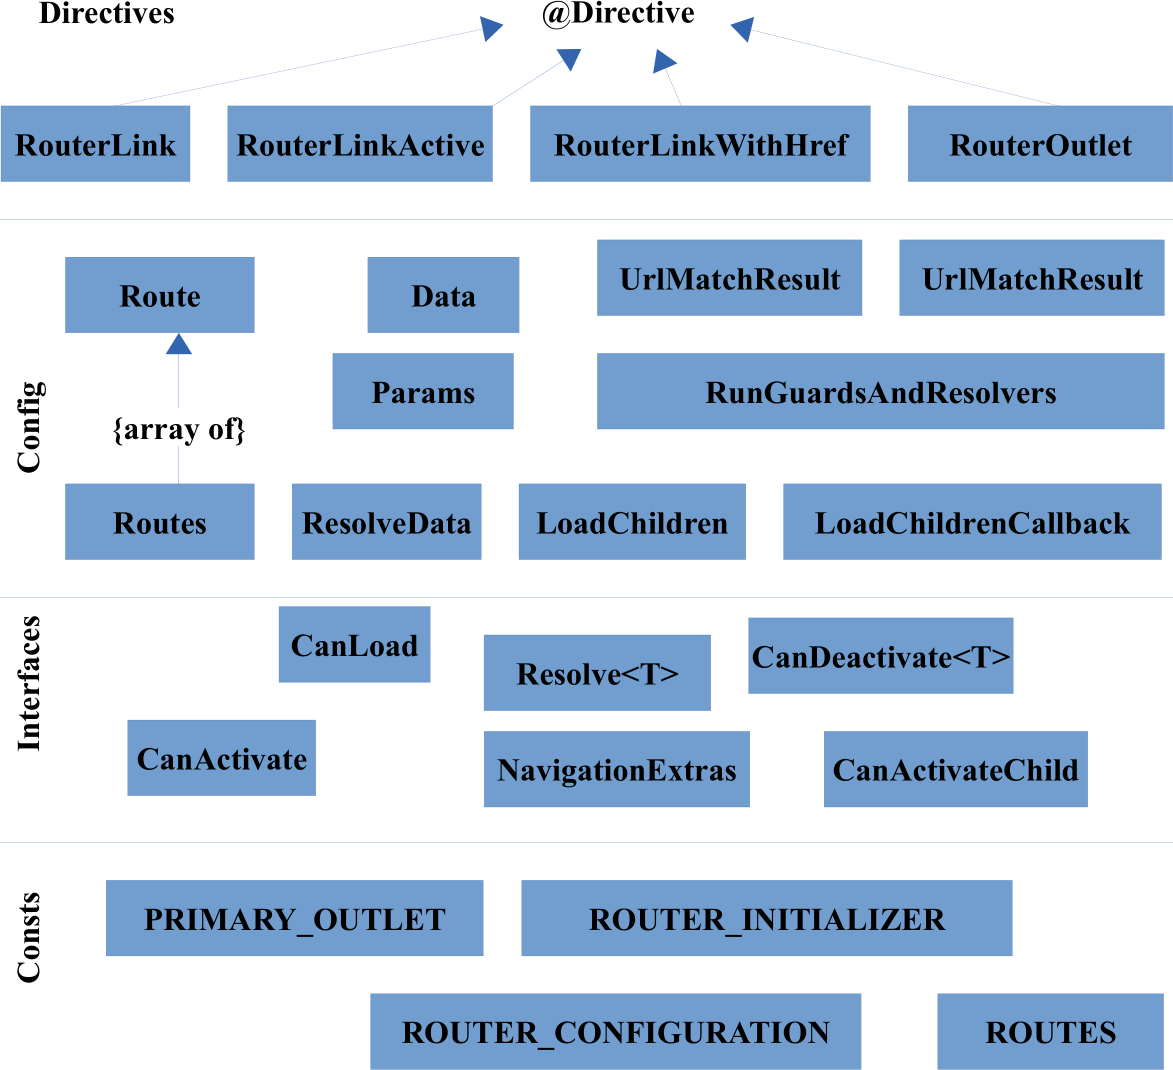
\includegraphics[width=0.65\linewidth]{13_the_router_package/router_api_1}
  \label{fig:router_api_1}
\end{figure}

\begin{figure}[!hbt]
  \centering
  \caption{Angular Router API (part 2)}
  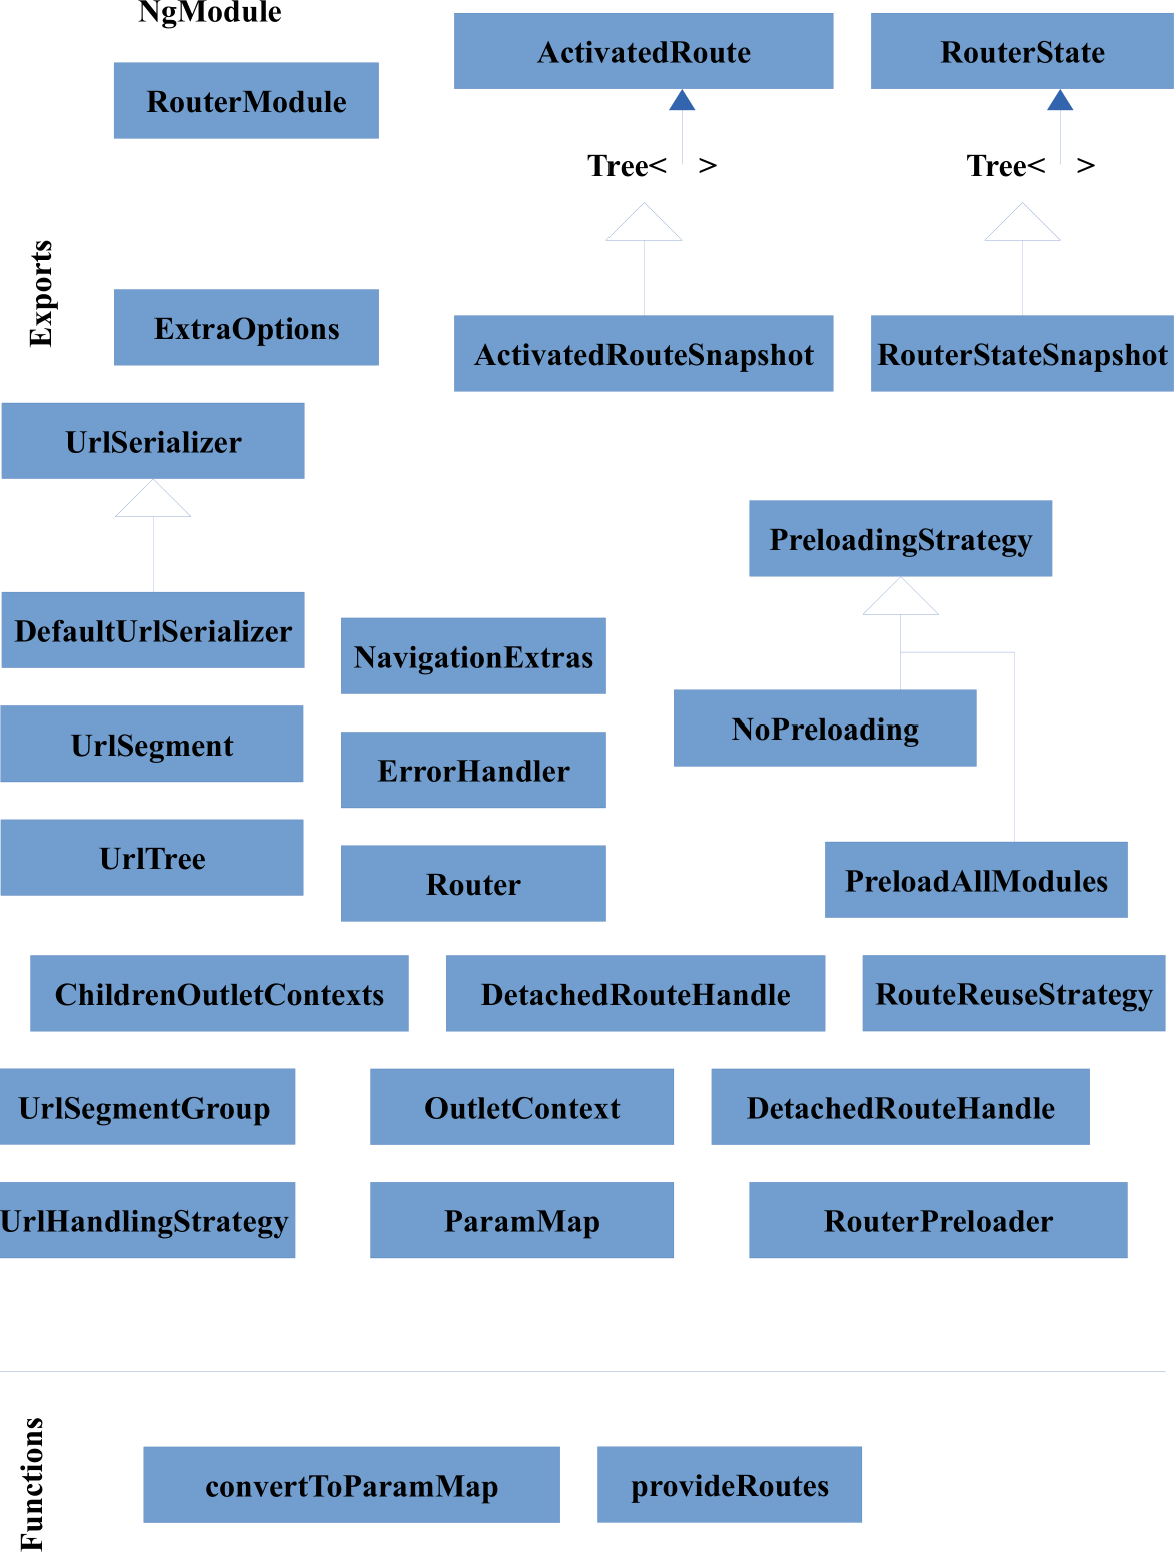
\includegraphics[width=0.75\linewidth]{13_the_router_package/router_api_2}
  \label{fig:router_api_2}
\end{figure}

\clearpage

\begin{figure}[!hbt]
  \centering
  \caption{Angular Router API (part 2)}
  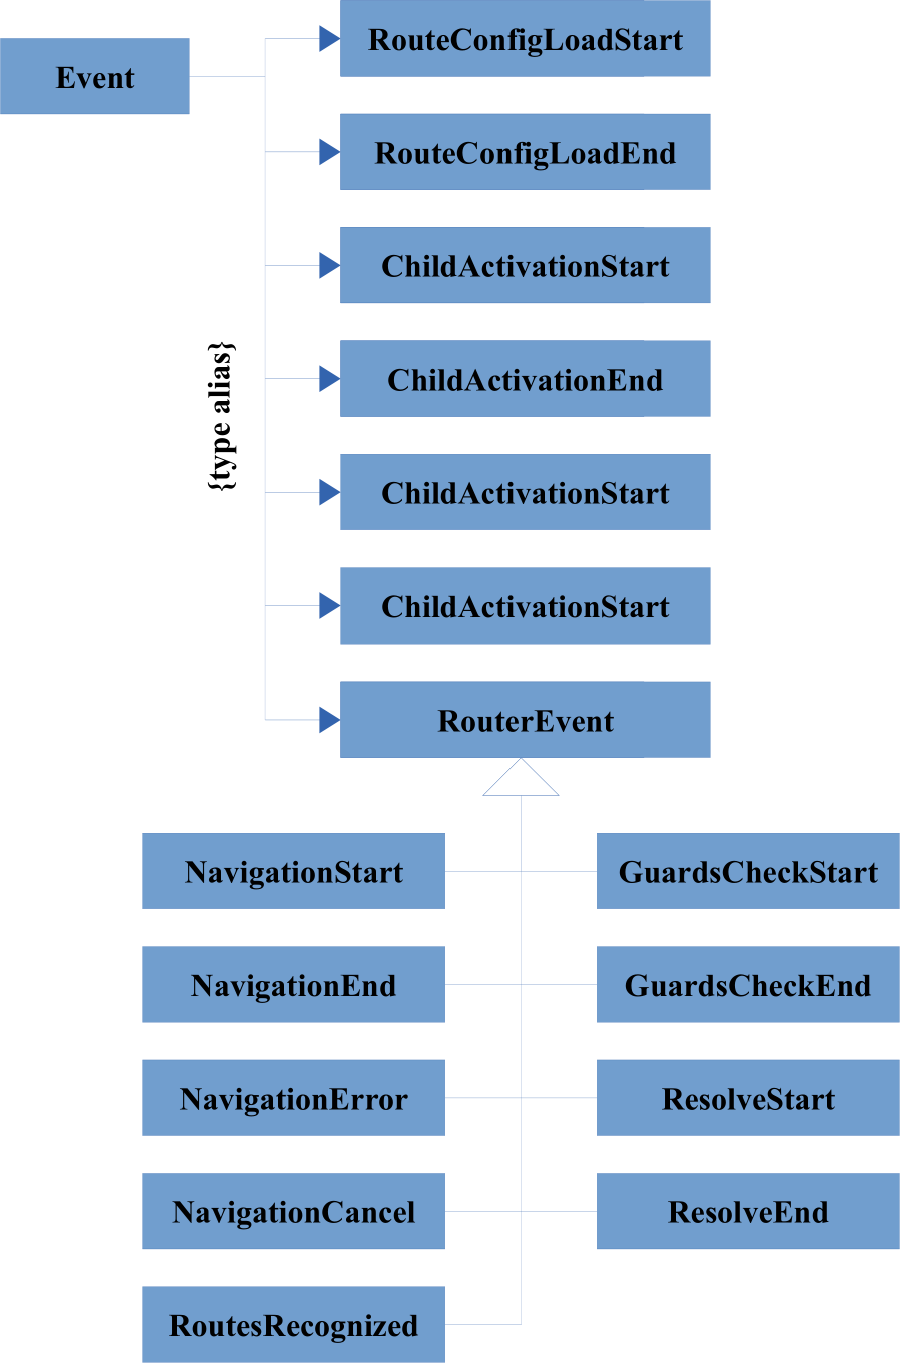
\includegraphics[width=0.75\linewidth]{13_the_router_package/router_api_3}
  \label{fig:router_api_3}
\end{figure}

\clearpage

% The Angular Router source tree is at:

Angular Router 源码位于:

\begin{itemize}
  \item \href{https://github.com/angular/angular/tree/master/packages/router}
        {<ANGULAR-MASTER>/packages/router}
\end{itemize}

% Its root directory contains index.ts, which just exports the contents of public\_api.ts,
% which in turn exports the contents of .src/index.ts.

根目录包含 index.ts,它只是导出了 public\_api.t 的内容,
而后者又导出\, .src/index.ts 的内容。

% This lists the exports and gives an initial impression of the size of the router package:

这列出了 exports 内容并给出了路由器包大小的初步印象:

\begin{minted}{typescript}
export {
  Data,
  LoadChildren,
  LoadChildrenCallback,
  ResolveData,
  Route,
  Routes,
  RunGuardsAndResolvers,
  UrlMatchResult,
  UrlMatcher,
} from './config';
export { RouterLink, RouterLinkWithHref } from './directives/router_link';
export { RouterLinkActive } from './directives/router_link_active';
export { RouterOutlet } from './directives/router_outlet';
export {
  ActivationEnd,
  ActivationStart,
  ChildActivationEnd,
  ChildActivationStart,
  Event,
  GuardsCheckEnd,
  GuardsCheckStart,
  NavigationCancel,
  NavigationEnd,
  NavigationError,
  NavigationStart,
  ResolveEnd,
  ResolveStart,
  RouteConfigLoadEnd,
  RouteConfigLoadStart,
  RouterEvent,
  RoutesRecognized,
} from './events';
export {
  CanActivate,
  CanActivateChild,
  CanDeactivate,
  CanLoad,
  Resolve,
} from './interfaces';
export {
  DetachedRouteHandle,
  RouteReuseStrategy,
} from './route_reuse_strategy';
export { NavigationExtras, Router } from './router';
export { ROUTES } from './router_config_loader';
export {
  ExtraOptions,
  ROUTER_CONFIGURATION,
  ROUTER_INITIALIZER,
  RouterModule,
  provideRoutes,
} from './router_module';
export { ChildrenOutletContexts, OutletContext } from './router_outlet_context';
export {
  NoPreloading,
  PreloadAllModules,
  PreloadingStrategy,
  RouterPreloader,
} from './router_preloader';
export {
  ActivatedRoute,
  ActivatedRouteSnapshot,
  RouterState,
  RouterStateSnapshot,
} from './router_state';
export { PRIMARY_OUTLET, ParamMap, Params, convertToParamMap } from './shared';
export { UrlHandlingStrategy } from './url_handling_strategy';
export {
  DefaultUrlSerializer,
  UrlSegment,
  UrlSegmentGroup,
  UrlSerializer,
  UrlTree,
} from './url_tree';
export { VERSION } from './version';
\end{minted}


% It also has the line:

它还有一行:

\begin{minted}{typescript}
export * from './private_export';
\end{minted}


% As already discussed, such private exports are intended for other packages within the
% Angular Framework itself, and not to be directly used by Angular applications. The
% private\_export.ts file has these exports (note names are prepended with ’ ’);
% ɵ

正如已经讨论过的,此类私有导出旨在用于 Angular 框架本身,而不应该由 Angular 应用直接使用。
private\_export.ts 文件具有这些导出(注意,它们的名称有 “ɵ” 字符);

\begin{minted}{typescript}
export { ROUTER_PROVIDERS as ɵROUTER_PROVIDERS } from './router_module';
export { flatten as ɵflatten } from './utils/collection';
\end{minted}


\section{Source Tree Layout}

% The source tree for the Router package contains these directories:

\begin{itemize}
  \item scripts
  \item src
  \item test (unit tests in Jasmine)
  \item testing (testing tools)
\end{itemize}

% The Router package root directory contains these files:

\begin{itemize}
  \item BUILD.bazel
  \item index.ts
  \item karma-test-shim.ts
  \item karma.config.js
  \item LICENSE
  \item package.json
  \item public\_api.ts
  \item README.md
  \item rollup.config.js
  \item tsconfig-build.json
\end{itemize}

% \section{Source}
\section{源码}

\subsection{router/src}

The router/src directory contains:

\begin{itemize}
  \item apply\_redirects.ts
  \item config.ts
  \item create\_router\_state.ts
  \item create\_url\_tree.ts
  \item events.ts
  \item interfaces.ts
  \item index.ts
  \item interfaces.ts
  \item pre\_activation.ts
  \item private\_export.ts
  \item recognize.ts
  \item resolve.ts
  \item route\_reuse\_strategy.ts
  \item router\_config\_loader.ts
  \item router\_module.ts
  \item router\_outlet\_context.ts
  \item router\_preloader.ts
  \item router\_state.ts
  \item router.ts
  \item shared.ts
  \item url\_handling\_strategy.ts
  \item url\_tree.ts
  \item version.ts
\end{itemize}

We’ll start by looking at:

\begin{itemize}
  \item \href{https://github.com/angular/angular/blob/master/packages/router/src/router_module.ts}
        {<ANGULAR-MASTER>/packages/router/src/router\_module.ts}
\end{itemize}

which defines the RouterModule class and related types.

It defines three consts:

\input{13_the_router_package/code/13_3_0_0.tex}

The first,
\texttt{ROUTER\_DIRECTIVES}
, is the collection of router directives that can appear in
Angular templates defining where the routed content is to be located on the page, and
how links used for routing are to be displayed.
\texttt{ROUTER\_DIRECTIVES}
is specified in the
declarations and exports of the
\texttt{@NgModule}
metadata for
\texttt{RouterModule}
:

\input{13_the_router_package/code/13_3_0_1.tex}

The other two are injection tokens for DI:

\input{13_the_router_package/code/13_3_0_2.tex}

It also defines the
\texttt{ROUTER\_PROVIDERS}
array of providers (which is only used by
forRoot, not forChild):

\input{13_the_router_package/code/13_3_0_3.tex}

An important provider there is
\texttt{Router}
, which is the actually routing service. This is set
up in DI to return the result of the
\texttt{setupRouter}
factory method. An abbreviated
version of this is as follows:

\input{13_the_router_package/code/13_3_0_4.tex}

It instantiates the router service and for each specified option / strategy takes
appropciarte action. Then it returns the new router service instance. It is important
that there is only a single router service per application the web browser only have a
single URL per session) and we need to track how this is so.

RouterModule is defined as:

\input{13_the_router_package/code/13_3_0_5.tex}

Note that both
\texttt{forRoot}
and
\texttt{forChild}
return a
\texttt{ModuleWithProviders}
instance. What
they put in it is different. Recall that this type is defined in:

\begin{itemize}
  \item \href{https://github.com/angular/angular/blob/master/packages/core/src/metadata/ng_module.ts}
        {<ANGULAR-MASTER>/packages/core/src/metadata/ng\_module.ts}
\end{itemize}

as follows:

\input{13_the_router_package/code/13_3_0_6.tex}

\texttt{ForChild}
is intended for all except the root routing module. It returns
\texttt{ngModule}
and a
list of providers that only contains the result of calling
\texttt{provideRoutes}
:

\input{13_the_router_package/code/13_3_0_7.tex}

Critically, it does not contain ROUTER\_PROVIDERS. In contrast,
\texttt{forRoot}
adds this and
many more providers:

\input{13_the_router_package/code/13_3_0_8.tex}

\texttt{ExtraOptions}
are additional options passed in to
\texttt{forRoot}
(it is not used with
\texttt{forChild}
):

\input{13_the_router_package/code/13_3_0_9.tex}

For example, if we wished to customize how preloading worked, we need to set the
\texttt{preloadingStrategy}
option.

The
\texttt{provideRouterInitializer()}
function providers a list of initializers:

\input{13_the_router_package/code/13_3_0_10.tex}

This uses the
\texttt{RouterInitializer}
class, whose purpose is best explained by this
comment in the code:

\input{13_the_router_package/code/13_3_0_11.tex}

We saw when examining the Core package that its:

\begin{itemize}
  \item \href{https://github.com/angular/angular/blob/master/packages/core/src/application_init.ts}
        {<ANGULAR\_MASTER>/packages/core/src/application\_init.ts}
\end{itemize}

defines
\texttt{APP\_INITIALIZER}
as:

\input{13_the_router_package/code/13_3_0_12.tex}

Interfaces.ts declares a number of useful interfaces.

\input{13_the_router_package/code/13_3_0_13.tex}

router\_config\_loader.ts defines a class -
\texttt{RouterConfigLoader}
– and an opaque token,
\texttt{ROUTES}
.  After some bookkeeping,
\texttt{RouterConfigLoader}
creates a new instance of
LoadedRouterConfig it:

\input{13_the_router_package/code/13_3_0_14.tex}

The router\_state.ts file contains these classes (and some helper functions):

\begin{itemize}
  \item RouterState
  \item ActivatedRoute
  \item ActivatedRouteSnapshot
  \item RouterStateSnapshot
\end{itemize}

\texttt{RouterState}
is defined as:

\input{13_the_router_package/code/13_3_0_15.tex}

\texttt{RouterStateSnapshot}
is defined as:

\input{13_the_router_package/code/13_3_0_16.tex}

The
\texttt{setRouterStateSnapshot()}
function is defined as:

\input{13_the_router_package/code/13_3_0_17.tex}

So its sets the router state for the current node, and then recursively calls
\texttt{setRouterState()}
to set it for all children.

The
\texttt{ActivatedRoute}
class is used by the router outlet directive to describe the
component it has loaded:

\input{13_the_router_package/code/13_3_0_18.tex}

\subsection{router/src/directives}

% This directory has the following files:

\begin{itemize}
  \item router\_link.ts
  \item router\_link\_active.ts
  \item router\_outlet.ts
\end{itemize}

% The router\_link.ts file contains the
% \texttt{RouterLink}
% directive:

\input{13_the_router_package/code/13_3_1_0.tex}

% The router link commands are set via:

\input{13_the_router_package/code/13_3_1_1.tex}

% When the link is clicked, the
% \texttt{onClick()}
% method is called:

\input{13_the_router_package/code/13_3_1_2.tex}

% The urlTree getter uses
% \texttt{Router.createlUrlTree()}
% :

\input{13_the_router_package/code/13_3_1_3.tex}

% The same file also contains the
% \texttt{RouterLinkWithHref}
% directive:

\input{13_the_router_package/code/13_3_1_4.tex}

% This has a href:

\input{13_the_router_package/code/13_3_1_5.tex}

% and manages the
% \texttt{urlTree}
% as a field and sets it from the constructor via a call to:

\input{13_the_router_package/code/13_3_1_6.tex}

% The router\_link\_active.ts file contains the
% \texttt{RouterLinkActive}
% directive:

\input{13_the_router_package/code/13_3_1_7.tex}

% This is used to add a CSS class to an element representing an active route. Its
% constructor is defiend as:

\input{13_the_router_package/code/13_3_1_8.tex}

% Its
% \texttt{update}
% method uses the configured renderer to set the element class:

\input{13_the_router_package/code/13_3_1_9.tex}

% The router\_outlet.ts file contains the
% \texttt{RouterOutlet}
% class:

\input{13_the_router_package/code/13_3_1_10.tex}

% This is where application component whose lifecycle depends on the router live. We
% note the
% \texttt{ViewContainerRef}
% 1
% and
% \texttt{ComponentFactoryResolver}
% 2
% parameters to the
% constructor.

% \texttt{ngOnInit}
% will either call
% \texttt{attach}
% 1
% or
% \texttt{activateWith}
% 2
% , depending on whether there is
% an existing component:

\input{13_the_router_package/code/13_3_1_11.tex}

% attach is defined as:

\input{13_the_router_package/code/13_3_1_12.tex}

% When its activateWith method is called, the resolver will be asked to resolve a
% component factory for the component:

\input{13_the_router_package/code/13_3_1_13.tex}

% The location field is of type
% \texttt{ViewContainerRef,}
% which we saw being set in the
% constructor.
% \texttt{ViewContainerRef}
% is defined in:

\begin{itemize}
  \item \href{https://github.com/angular/angular/blob/master/packages/core/src/linker/view_container_ref.ts}
        {<ANGULAR-MASTER>/packages/core/src/linker/view\_container\_ref.ts}
\end{itemize}

\input{13_the_router_package/code/13_3_1_14.tex}

% So the component is appended as the last entry in the
% \texttt{ViewContainer}
% .



% \chapter{Render3 (Ivy) in Angular}
\chapter{Render3 (Ivy) in Angular}

\section{Preliminaries – Paths and names}

% This document is a guided tour of the new “Ivy” rendering functionality within the
% modern Angular source tree. We mostly look at the main Angular repository (paths
% within which we prefix with ANGULAR-MASTER) and also have some discussion of the
% Angular CLI repository (paths within which we prefix with ANGULAR-CLI-MASTER).
% You may wish to clone these repositories to your local machine or you may wish to
% refer to them on Github. If the latter, you should expand these placeholders to:

\begin{itemize}
  \item ANGULAR-MASTER - https://github.com/angular/angular
  \item ANGUALR-CLI-MASTER - https://github.com/angular/angular-cli
\end{itemize}

% We like to use the name “Render3” (instead of “Render 3” with a space), as it helps
% with Google search, etc. The code-name for this is “Ivy”, we will see that used in
% places in the code and with the new
% \texttt{enableIvy}
% option for Compiler-CLI, which can be
% added via Angular CLI’s
% \texttt{ng new}
% command, as described here:

\begin{itemize}
  \item \url{https://next.angular.io/guide/ivy}
\end{itemize}

\section{Overview}

Rendering in Angular is undergoing further evolution. It seems it was not too long ago
that Angular 2’s original Render architecture evolved to Render2, and now along
comes the very new Render3, quite a different approach to a view engine.

The main change can be summed up with just this one function
(from
\href{https://github.com/angular/angular/blob/master/packages/core/src/render3/interfaces/renderer.ts}
{<ANGULAR-MASTER>/packages/core/src/render3/interfaces/renderer.ts}
):

\begin{minted}{typescript}
export const domRendererFactory3: RendererFactory3 = {
  createRenderer: (
    hostElement: RElement | null,
    rendererType: RendererType2 | null
  ): Renderer3 => {
    return document;
  } %\step{1}%,
};
\end{minted}


By default, the new renderer is compatible with the
\texttt{document}
object from the
standard DOM. Actually, it is better not just to say “compatible with” but to say “is”.
When running in the browser UI thread, where the DOM is available, then the
browser’s native
\texttt{document}
object (provided by the web browser itself, not Angular)
really IS the renderer – it is directly used to render content. An app literally cannot
perform quicker than that. Regardless of which framework you use and how it
structures its rendering pipeline, ultimately this
\texttt{document}
object in the real DOM will
have to be called. So why not call it directly in scenarios where it is supported (that
means inside the browser UI thread)? That is exaclty what Ivy does when possible.
For other rendering scenarios (web worker, server, or more specialized, such as
WebRTC) then something that looks like the
\texttt{document}
object will need to be provided.

For readers coming from a C++, C\#, Java or similar background, it is very important
to understand that TypeScript (and JavaScript) uses
\url{structuralsubtyping}
(also
affectionately called “duck typing”) and not nominal typing (named types) as used by
those other languages. In TypeScript, a type that implements the fields of another
type can be used in its place – there is no neccessity for implementing common
interfaces or to have a common parent class. So the fact that the
\texttt{document}
object
from the standard DOM does not implement Angular’s
\texttt{Render3}
but yet is being used
in a function to return such a type (see
1
above), is not a problem, so long as it
implements all the fields that
\texttt{Render3}
needs (which it does, as we shall soon
discover).

Now we will explore in more depth what is happening when we use
\texttt{enableIvy}
with
Angular CLI and how the main Angular project delivers Render3 functionality. We will
see three of its packages are involved – Compiler-CLI, Compiler and Core.

% \subsection{Public Documentation}
\subsection{公共文档}

% If we visit:

如果我们访问:

\begin{itemize}
  \item \url{https://next.angular.io/api?query=render}
\end{itemize}

% we see the following listing for all parts of the public API that contain the term
% “render”:

我们将会看到所有包含 “render” 关键字的公共 API 列表

% So for now, there is no public API to any Renderer3 functionality.

所以目前,没有任何 Renderer3 功能的公共 API。


% \subsection{Public Documentation}
\subsection{公共文档}

% If we visit:

如果我们访问:

\begin{itemize}
  \item \url{https://next.angular.io/api?query=render}
\end{itemize}

% we see the following listing for all parts of the public API that contain the term
% “render”:

我们将会看到所有包含 “render” 关键字的公共 API 列表

% So for now, there is no public API to any Renderer3 functionality.

所以目前,没有任何 Renderer3 功能的公共 API。


\section{The Angular CLI And enableIvy}

Application developers wishing to use Ivy will mostly do so via the
\emph{enableIvy}
command line option to Angular CLI:

\begin{itemize}
  \item \url{https://next.angular.io/guide/ivy}
\end{itemize}

We can see from the Angular CLI 8.2 source tree this option impacts the code base in
a few places. The schema for Angular Application options is defined here:

\begin{itemize}
  \item \href{https://github.com/angular/angular-cli/blob/master/packages/schematics/angular/application/schema.json}
        {<ANGULAR-CLI-MASTER>/packages/schematics/angular/application/schema.json}
\end{itemize}

and includes this for
\texttt{enableIvy}
:

\begin{minted}{json}
{
  "$schema": "http://json-schema.org/schema",
  "id": "SchematicsAngularApp",
  "title": "Angular Application Options Schema",
  "type": "object",
  "description": "Generates a new basic app definition in the \"projects\" subfolder of the workspace.",
  "properties": {
    "enableIvy": {
      "description": "**EXPERIMENTAL** True to create a new app that uses the Ivy rendering engine.",
      "type": "boolean",
      "default": false,
      "x-user-analytics": 8
\end{minted}


The entry point for Angular Application schematics:

\begin{itemize}
  \item \href{https://github.com/angular/angular-cli/blob/master/packages/schematics/angular/application/index.ts}
        {<ANGULAR-CLI-MASTER>/packages/schematics/angular/application/index.ts}
\end{itemize}

has this code :

\begin{minted}{typescript}
const project = {
  root: normalize(projectRoot),
  sourceRoot,
  projectType: ProjectType.Application,
  prefix: options.prefix || 'app',
  schematics,
  targets: {
    build: {
      builder: Builders.Browser,
      options: {
        ..
        aot: !!options.enableIvy,
        ..
      }, ..
    }, ..
  }, ..
};
\end{minted}


The schema for Angular Ng New options is defined here:
enableIvy option set
in tsconfig.app.json

\begin{itemize}
  \item \href{https://github.com/angular/angular-cli/blob/master/packages/schematics/angular/ng-new/schema.json}
        {<ANGULAR-CLI-MASTER>/packages/schematics/angular/ng-new/schema.json}
\end{itemize}

and has these entries:

\begin{minted}{ts}
 {
  "$schema": "http://json-schema.org/schema",
  "id": "SchematicsAngularNgNew",
  "title": "Angular Ng New Options Schema",
  "type": "object",
  "properties": {
    "enableIvy": {
      "description":
          "When true, creates a new app that uses the Ivy rendering engine.",
      "type": "boolean",
      "default": false
    },
\end{minted}


The description string from above ends up here in the generated documentation:

\begin{itemize}
  \item \url{https://next.angular.io/cli/new}
\end{itemize}

The
\texttt{ng-new}
entrypoint:

\begin{itemize}
  \item \href{https://github.com/angular/angular-cli/blob/master/packages/schematics/angular/ng-new/index.ts}
        {<ANGULAR-CLI-MASTER>/packages/schematics/angular/ng-new/index.ts}
\end{itemize}

accepts the
\texttt{enableIvy}
parameter as follows:

\begin{minted}{typescript}
const applicationOptions: ApplicationOptions = {
  projectRoot: '',
  name: options.name,
  enableIvy: options.enableIvy,
  ...
  ..
};
\end{minted}


The template for tsconfig.app.json reacts to
\texttt{enableIvy}
if present:

\begin{itemize}
  \item \href{https://github.com/angular/angular-cli/blob/master/packages/schematics/angular/application/files/tsconfig.app.json.template}
        {<ANGULAR-CLI-MASTER>/packages/schematics/angular/application/files/tsconfig.app.json.template}
\end{itemize}

as it has this entry:

\begin{minted}{shell}
<%\%% if (enableIvy) { %\%%>,
  "angularCompilerOptions": {
    "enableIvy": true
  }<%\%% } %\%%>
\end{minted}


So that is how the entry gets into tsconfig.app.json. Now let’s see what impact it has.
The ngtools functionality for webpack configures the bootstrap code slightly differently
when
\texttt{enableIvy}
is enabled. In this file:

\begin{itemize}
  \item \href{https://github.com/angular/angular-cli/blob/master/packages/ngtools/webpack/src/transformers/replace_bootstrap.ts}
        {<ANGULAR-CLI-MASTER>/packages/ngtools/webpack/src/transformers/replace\_bootstrap.ts}
\end{itemize}

we see:

\begin{minted}{ts}
export function replaceBootstrap(
  ..,
  enableIvy?: boolean,
): ts.TransformerFactory<ts.SourceFile> {
..
if (!enableIvy) {
        className += 'NgFactory';
        modulePath += '.ngfactory';
        bootstrapIdentifier = 'bootstrapModuleFactory';
      }
  ..
}
\end{minted}


So when
\texttt{enableIvy}
is NOT present, the names for the factory artefacts are different.
From where does
\texttt{replaceBootstrap}
get called? When we examine:

\begin{itemize}
  \item \href{https://github.com/angular/angular-cli/blob/master/packages/ngtools/webpack/src/angular_compiler_plugin.ts}
        {<ANGULAR-CLI-MASTER>/packages/ngtools/webpack/src/angular\_compiler\_plugin.ts}
\end{itemize}

we see the
\texttt{\_makeTransformers}
method is as follows:

\begin{minted}{typescript}
  private _makeTransformers() {
    ..
    if (this._platformTransformers !== null) {
      this._transformers.push(...this._platformTransformers);
    } else {
      if (this._platform === PLATFORM.Browser) {
        ..
        if (!this._JitMode) {
          // Replace bootstrap in browser AOT.
          this._transformers.push(
            replaceBootstrap(
              isAppPath,
              getEntryModule,
              getTypeChecker,
              !!this._compilerOptions.enableIvy
            )
          );
        }
      } else if (this._platform === PLATFORM.Server) {
        ..
      }
    } ..
  }
\end{minted}


We also see ivy used in
\texttt{\_processLazyRoutes}
:

\begin{minted}{typescript}
  // Process the lazy routes discovered, adding then to _lazyRoutes.
  // TODO: find a way to remove lazy routes that don't exist anymore.
  // This will require a registry of known references to a lazy route,
  // removing it when no
  // module references it anymore.
  private _processLazyRoutes(discoveredLazyRoutes: LazyRouteMap) {
    Object.keys(discoveredLazyRoutes).forEach((lazyRouteKey) => {
      ..
      if (
        this._JitMode ||
        // When using Ivy and not using allowEmptyCodegenFiles,
        // factories are not generated.
        (this._compilerOptions.enableIvy &&
          !this._compilerOptions.allowEmptyCodegenFiles)
      ) {
        modulePath = lazyRouteTSFile;
        moduleKey = `${lazyRouteModule}${moduleName ? '#' + moduleName : ''}`;
      } else {
        ..
      }
    });
  }
\end{minted}


We also see ivy impacting on how
\texttt{\_createOrUpdateProgram}
works:

\begin{minted}{typescript}
  private async _createOrUpdateProgram() {
    ..
    if (!this.entryModule && !this._compilerOptions.enableIvy) {
      this._warnings.push(
        'Lazy routes discovery is not enabled. ' +
          'Because there is neither an entryModule nor a ' +
          'statically analyzable bootstrap code in the main file.'
      );
    }
    ..
  }
\end{minted}


\subsection{Impact enableIvy has on Angular CLI’s code generation}

% To best see the differences the
% \texttt{enableIvy}
% option has on code generation, we will now
% create two new projects – one with and one without the
% \texttt{--enableIvy}
% option. To save
% us some time we will use the
% \texttt{–-skipInstall}
% option, which means npm install is not
% run to download all the dependency packages.

\input{14_render_ivy_in_angular/code/14_2_0_0.tex}

% A search for
% \texttt{ivy}
% in the generated render2 codebase reveals no hits, as expected. A
% search for
% \texttt{ivy}
% in the render3 codebase reveals 2 hits. In package.json,
% \texttt{scripts}
% has
% this additional item:

\input{14_render_ivy_in_angular/code/14_2_0_1.tex}

% and in tsconfig.app.json,
% \texttt{angularCompilerOptions}
% has this entry:

\input{14_render_ivy_in_angular/code/14_2_0_2.tex}

% Now that we have seen how Angular CLI adds enableIvy, we are ready to move on to
% explore how Compiler CLI detects and reacts to this.


\subsection{Impact enableIvy has on Angular CLI’s code generation}

% To best see the differences the
% \texttt{enableIvy}
% option has on code generation, we will now
% create two new projects – one with and one without the
% \texttt{--enableIvy}
% option. To save
% us some time we will use the
% \texttt{–-skipInstall}
% option, which means npm install is not
% run to download all the dependency packages.

\input{14_render_ivy_in_angular/code/14_2_0_0.tex}

% A search for
% \texttt{ivy}
% in the generated render2 codebase reveals no hits, as expected. A
% search for
% \texttt{ivy}
% in the render3 codebase reveals 2 hits. In package.json,
% \texttt{scripts}
% has
% this additional item:

\input{14_render_ivy_in_angular/code/14_2_0_1.tex}

% and in tsconfig.app.json,
% \texttt{angularCompilerOptions}
% has this entry:

\input{14_render_ivy_in_angular/code/14_2_0_2.tex}

% Now that we have seen how Angular CLI adds enableIvy, we are ready to move on to
% explore how Compiler CLI detects and reacts to this.


\section{Render3 In The Compiler-CLI Package}

% Despite its name, Compiler CLI is both a set of command-line interfaces and an API (a
% library). It has three apps, that we see defined in:

\begin{itemize}
  \item \href{https://github.com/angular/angular/blob/master/packages/compiler-cli/package.json}
        {<ANGULAR-MASTER>/packages/compiler-cli/package.json}
\end{itemize}

% as follows, which lists their entry points:

\begin{minted}{json}
  "bin": {
    "ngc": "./src/main.js",
    "ivy-ngcc": "./src/ngcc/main-ngcc.js",
    "ng-xi18n": "./src/extract_i18n.js"
  },
\end{minted}


% Ngc is the main Angular template compiler, ivy-ngcc is the Angular Compatibility
% Compiler and ng-xi18n is for internationalization.

% As a library, Compiler CLI mostly exports types from the Compiler package, as seen
% by its
% \url{index.ts}
% file, along with some useful diagnostics types, defined locally within
% Compiler CLI. The naming of none of these exports is Ivy-specific, but their internals
% are impacted by use of Ivy, as we shall soon see.

% In root of the src tree, there are references to Ivy in main.ts and perform\_compile.ts.

% \url{main.ts}
% has this:

\begin{minted}{typescript}
function createEmitCallback(
  options: api.CompilerOptions
): api.TsEmitCallback | undefined {
  const transformDecorators =
    !options.enableIvy && options.annotationsAs !== 'decorators';
  ..
}
\end{minted}


% and this detailed error reporter:

\begin{minted}{typescript}
function reportErrorsAndExit(
  allDiagnostics: Diagnostics,
  options?: api.CompilerOptions,
  consoleError: (s: string) => void = console.error
): number {
  const errorsAndWarnings = filterErrorsAndWarnings(allDiagnostics);
  if (errorsAndWarnings.length) {
    const formatHost = getFormatDiagnosticsHost(options);
    if (options && options.enableIvy === true) {
      const ngDiagnostics = errorsAndWarnings.filter(api.isNgDiagnostic);
      const tsDiagnostics = errorsAndWarnings.filter(api.isTsDiagnostic);
      consoleError(
        replaceTsWithNgInErrors(
          ts.formatDiagnosticsWithColorAndContext(tsDiagnostics, formatHost)
        )
      );
      consoleError(formatDiagnostics(ngDiagnostics, formatHost));
    } else {
      consoleError(formatDiagnostics(errorsAndWarnings, formatHost));
    }
  }
  return exitCodeFromResult(allDiagnostics);
}
\end{minted}


% \url{perform_compile.ts}
% has this:

\begin{minted}{typescript}
export function createNgCompilerOptions(
  basePath: string,
  config: any,
  tsOptions: ts.CompilerOptions
): api.CompilerOptions {
  // enableIvy `ngtsc` is an alias for `true`.
  if (
    config.angularCompilerOptions &&
    config.angularCompilerOptions.enableIvy === 'ngtsc'
  ) {
    config.angularCompilerOptions.enableIvy = true;
  }
  return {
    ...tsOptions,
    ...config.angularCompilerOptions,
    genDir: basePath,
    basePath,
  };
}
\end{minted}


% The CompilerOptions interface is defined in the transformers sub-directory. In:

\begin{itemize}
  \item \href{https://github.com/angular/angular/blob/master/packages/compiler-cli/src/transformers/api.ts}
        {<ANGULAR-MASTER>/packages/compiler-cli/src/transformers/api.ts}
\end{itemize}

% we see it defines an interface,
% \texttt{CompilerOptions}
% , that extends
% \texttt{ts.CompilerOptions}
% with Angular-specific fields.

\begin{minted}{typescript}
export interface CompilerOptions extends ts.CompilerOptions {
  // NOTE: These comments and aio/content/guides/aot-compiler.md
  // should be kept in sync.
  ..
}
\end{minted}


% Despite this comment about aot-compiler.md, that Markdown file actually contains no
% mention of Ivy. The
% \texttt{CompilerOptions}
% interface in api.ts does contain this addition:

\begin{minted}{ts}
  /**
   * Tells the compiler to generate definitions using the Render3 style code
   * generation. This option defaults to `false`.
   *
   * Not all features are supported with this option enabled. It is only
   * supported for experimentation and testing of Render3 style code
   * generation.
   * Acceptable values are as follows:
   *
   * `false` - run ngc normally
   * `true` - run the ngtsc compiler instead of the normal ngc compiler
   * `ngtsc` - alias for `true`
   * `tsc` - behave like plain tsc as much as possible
   *         (used for testing JIT code)
   *
   * @publicApi
   */
 enableIvy?: boolean|'ngtsc'|'tsc';
}
\end{minted}


% So we see there is a new ngtsc compiler in addition to the normal tsc compiler, and
% this switch is used to select one or the other. We will soon explore how ngtsc works.

% The api.ts file also defines
% \texttt{EmitFlags}
% , which is of interest to us (note the
% \texttt{default}
% includes codegen):

\begin{minted}{typescript}
export enum EmitFlags {
  DTS = 1 << 0,
  JS = 1 << 1,
  Metadata = 1 << 2,
  I18nBundle = 1 << 3,
  Codegen = 1 << 4,
  Default = DTS | JS | Codegen,
  All = DTS | JS | Metadata | I18nBundle | Codegen,
}
\end{minted}


% The tsc\_pass\_through.ts file defines an implementation of the Program API:

\begin{minted}{typescript}
import { ivySwitchTransform } from '../ngtsc/switch';

/**
 * An implementation of the `Program` API which behaves similarly to plain `
 * tsc`. The only Angular specific behavior included in this `Program` is the
 * operation of the Ivy switch to turn on render3 behavior. This allows `ngc`
 * to behave like `tsc` in cases where JIT code needs to be tested.
 */
export class TscPassThroughProgram implements api.Program {
  ...
  emit(opts?: {
    ..
  }): ts.EmitResult {
    const emitCallback = (opts && opts.emitCallback) || defaultEmitCallback;
    const emitResult = emitCallback({
      ..
      customTransformers: { before: [ivySwitchTransform] },
    });
    return emitResult;
  }
}
\end{minted}


% We see Ivy impacting the program.ts file in a number of ways.

\begin{itemize}
  \item \href{https://github.com/angular/angular/blob/master/packages/compiler-cli/src/transformers/program.ts}
        {<ANGULAR-MASTER>/packages/compiler-cli/src/transformers/program.ts}
\end{itemize}

% The command line option is extracted in
% \texttt{getAotCompilerOptions()}
% :

\begin{minted}{typescript}
// Compute the AotCompiler options
function getAotCompilerOptions(options: CompilerOptions): AotCompilerOptions {
  ..
  return {
    ..
    enableIvy: options.enableIvy,
  };
}
\end{minted}


% Metadata is expected to be lower case:

\begin{minted}{ts}
// Fields to lower within metadata in render2 mode.
const LOWER_FIELDS =
                ['useValue', 'useFactory', 'data', 'id', 'loadChildren'];
// Fields to lower within metadata in render3 mode.
const R3_LOWER_FIELDS = [...LOWER_FIELDS, 'providers', 'imports', 'exports'];

class AngularCompilerProgram implements Program {
  constructor(
  …
    this.loweringMetadataTransform =
               new LowerMetadataTransform(
                       options.enableIvy ? R3_LOWER_FIELDS : LOWER_FIELDS);
\end{minted}


% Also in
% \texttt{AngularCompilerProgram}
% we see the use of reified decorators for Render3:

\begin{minted}{typescript}
  R3_REIFIED_DECORATORS = [
    'Component',
    'Directive',
    'Injectable',
    'NgModule',
    'Pipe',
  ];

  private get reifiedDecorators(): Set<StaticSymbol> {
    if (!this._reifiedDecorators) {
      const reflector = this.compiler.reflector;
      this._reifiedDecorators = new Set(
        R3_REIFIED_DECORATORS.map((name) =>
          reflector.findDeclaration('@angular/core', name)
        )
      );
    }
    return this._reifiedDecorators;
  }
\end{minted}


% The
% \texttt{emit}
% method has protection against being inadvertently called for Ivy:

\begin{minted}{typescript}
  emit(
    parameters: {
      emitFlags?: EmitFlags;
      cancellationToken?: ts.CancellationToken;
      customTransformers?: CustomTransformers;
      emitCallback?: TsEmitCallback;
      mergeEmitResultsCallback?: TsMergeEmitResultsCallback;
    } = {}
  ): ts.EmitResult {
    if (this.options.enableIvy) {
      throw new Error('Cannot run legacy compiler in ngtsc mode');
    }
    return this._emitRender2(parameters);
  }
\end{minted}


% The createProgram function is where the decision is made which compilation program
% to use; this is influenced by the value for enableIvy:

\begin{minted}{typescript}
export function createProgram({
  rootNames,
  options,
  host,
  oldProgram,
}: {
  rootNames: ReadonlyArray<string>;
  options: CompilerOptions;
  host: CompilerHost;
  oldProgram?: Program;
}): Program {
  if (options.enableIvy === true) {
    return new NgtscProgram(rootNames, options, host, oldProgram);
  } else if (options.enableIvy === 'tsc') {
    return new TscPassThroughProgram(rootNames, options, host, oldProgram);
  }
  return new AngularCompilerProgram(rootNames, options, host, oldProgram);
}
\end{minted}


% Before leaving program.ts, we wish to mention two other functions. This file also
% contains the
% \texttt{defaultEmitCallback}
% :

\begin{minted}{typescript}
const defaultEmitCallback: TsEmitCallback = ({
  program,
  targetSourceFile,
  writeFile,
  cancellationToken,
  emitOnlyDtsFiles,
  customTransformers,
}) =>
  %\step{1}% program.emit(
    targetSourceFile,
    writeFile,
    cancellationToken,
    emitOnlyDtsFiles,
    customTransformers
  );
\end{minted}


% We see at
% 1
% where the compilation is actually initiated with the set of custom
% transformers which was passed in as a parameter.
% One other important helper function is
% \texttt{calculateTransforms()}
% , defined as:

\begin{minted}{typescript}
  private calculateTransforms(
    genFiles: Map<string, GeneratedFile> | undefined,
    partialModules: PartialModule[] | undefined,
    stripDecorators: Set<StaticSymbol> | undefined,
    customTransformers?: CustomTransformers
  ): ts.CustomTransformers {
    ...
    %\step{1}% if (partialModules) {
      beforeTs.push(getAngularClassTransformerFactory(partialModules));
      ..
    } ..
  }
\end{minted}


% We see at
% 1
% how those partial modules are processed. In particular, we see the use of
% the new
% \texttt{getAngularClassTransformerFactory}
% function. It is defined in:

\begin{itemize}
  \item \href{https://github.com/angular/angular/blob/c8a1a14b87e5907458e8e87021e47f9796cb3257/packages/compiler-cli/src/transformers/r3_transform.ts}
        {<ANGULAR-MASTER>/packages/compiler-cli/src/transformers/r3\_transform.ts}
\end{itemize}

% as follows:

\begin{minted}{typescript}
/**
 * Returns a transformer that adds the requested static methods
 * specified by modules.
 */
export function getAngularClassTransformerFactory(
  modules: PartialModule[]
): TransformerFactory {
  if (modules.length === 0) {
    // If no modules are specified, just return an identity transform.
    return () => (sf) => sf;
  }
  const moduleMap = new Map(
    modules.map<[string, PartialModule]>((m) => [m.fileName, m])
  );
  return function (context: ts.TransformationContext) {
    return function (sourceFile: ts.SourceFile): ts.SourceFile {
      const module = moduleMap.get(sourceFile.fileName);
      if (module) {
        const [newSourceFile] = updateSourceFile(sourceFile, module, context);
        return newSourceFile;
      }
      return sourceFile;
    };
  };
}
\end{minted}


% Two important types are also defined in r3\_transform.ts to describe what a
% \texttt{Transformer}
% and a
% \texttt{TransformerFactory}
% are:

\begin{minted}{typescript}
export type Transformer = (sourceFile: ts.SourceFile) => ts.SourceFile;
export type TransformerFactory = (
  context: ts.TransformationContext
) => Transformer;
\end{minted}


% The
% \texttt{PartialModuleMetadataTransformer}
% function is defined in:

\begin{itemize}
  \item \href{https://github.com/angular/angular/blob/master/packages/compiler-cli/src/transformers/r3_metadata_transform.ts}
        {<ANGULAR-MASTER>/packages/compiler-cli/src/transformers/r3\_metadata\_transform.ts}
\end{itemize}

% as:

\begin{minted}{typescript}
export class PartialModuleMetadataTransformer implements MetadataTransformer {
  private moduleMap: Map<string, PartialModule>;

  constructor(modules: PartialModule[]) {
    this.moduleMap = new Map(
      modules.map<[string, PartialModule]>((m) => [m.fileName, m])
    );
  }

  start(sourceFile: ts.SourceFile): ValueTransform | undefined {
    const partialModule = this.moduleMap.get(sourceFile.fileName);
    if (partialModule) {
      const classMap = new Map<string, ClassStmt>(
        partialModule.statements
          .filter(isClassStmt)
          .map<[string, ClassStmt]>((s) => [s.name, s])
      );
      if (classMap.size > 0) {
        return (value: MetadataValue, node: ts.Node): MetadataValue => {
          // For class metadata that is going to be transformed to have a
          // static method ensure the metadata contains a
          // static declaration the new static method.
          if (
            isClassMetadata(value) &&
            node.kind === ts.SyntaxKind.ClassDeclaration
          ) {
            const classDeclaration = node as ts.ClassDeclaration;
            if (classDeclaration.name) {
              const partialClass = classMap.get(classDeclaration.name.text);
              if (partialClass) {
                for (const field of partialClass.fields) {
                  if (
                    field.name &&
                    field.modifiers &&
                    field.modifiers.some(
                      (modifier) => modifier === StmtModifier.Static
                    )
                  ) {
                    value.statics = {
                      ...(value.statics || {}),
                      [field.name]: {},
                    };
                  }
                }
              }
            }
          }
          return value;
        };
      }
    }
  }
}
\end{minted}


% Now we are ready go back to Compiler-CLI’s
% \url{program.ts}
% file to look at:

\begin{minted}{ts}
private _emitRender3(
1    {emitFlags = EmitFlags.Default, cancellationToken, customTransformers,
2     emitCallback = defaultEmitCallback}: {
        emitFlags?: EmitFlags,
        cancellationToken?: ts.CancellationToken,
        customTransformers?: CustomTransformers,
        emitCallback?: TsEmitCallback
 3  } = {}): ts.EmitResult {
    const emitStart = Date.now();

// .. Check emitFlags
// .. Set up code to emit partical modules
// .. Set up code for file writing (not shown)
// .. Build list of custom transformers
// .. Make emitResult
    return emitResult;
  }
\end{minted}


% This takes a range of input parameters (note
% \texttt{emitFlags}
% 1
% and
% \texttt{emitCallback}
% 2
% ) and
% then returns an instance of
% \texttt{ts.EmitResult}
% 3
% . The
% \texttt{emitFlags}
% says what needs to be
% emitted – if nothing, then we return immediately:

\begin{minted}{typescript}
if (
  (emitFlags &
    (EmitFlags.JS | EmitFlags.DTS | EmitFlags.Metadata | EmitFlags.Codegen)) ===
  0
) {
  return { emitSkipped: true, diagnostics: [], emittedFiles: [] };
}
\end{minted}


% The partial modules are processed with this important call to
% \texttt{emitAllPartialModules}
% in Angular’s Compiler package (we will examine this in detail
% shortly):

\begin{minted}{typescript}
const modules = this.compiler.emitAllPartialModules(this.analyzedModules);
\end{minted}


% The
% \texttt{this.analyzedModules}
% getter is defined as:

\begin{minted}{typescript}
  private get analyzedModules(): NgAnalyzedModules {
    if (!this._analyzedModules) {
      this.initSync();
    }
    return this._analyzedModules!; %\step{1}%
  }
\end{minted}


% Note the
% \texttt{!}
% at the end of the return
% 1
% : this is the TypeScript non-null assertion
% operator, a new language feature explained as:

% \emph{“A new ! post-fix expression operator may be used to assert that its operand}
% \emph{is non-null and non-undefined in contexts where the type checker is unable}
% \emph{to conclude that fact. Specifically, the operation x! produces a value of the}
% \emph{type of x with null and undefined excluded.” (}
% \emph{TypeScript release notes}
% \emph{)}

% The
% \texttt{\_analyzedModules}
% field is initialized earlier as:

\begin{minted}{typescript}
  private _analyzedModules: NgAnalyzedModules | undefined;
\end{minted}


% Returning to our coverage of
% \texttt{\_emitRender3}
% – after the call to
% \texttt{this.compiler.emitAllPartialModules}
% to emit the modules, the
% \texttt{writeTSFile}
% and
% \texttt{emitOnlyDtsFiles}
% consts are set up:

\begin{minted}{typescript}
const writeTsFile: ts.WriteFileCallback = (
  outFileName,
  outData,
  writeByteOrderMark,
  onError?,
  sourceFiles?
) => {
  const sourceFile =
    sourceFiles && sourceFiles.length == 1 ? sourceFiles[0] : null;
  let genFile: GeneratedFile | undefined;
  this.writeFile(
    outFileName,
    outData,
    writeByteOrderMark,
    onError,
    undefined,
    sourceFiles
  );
};

const emitOnlyDtsFiles =
  (emitFlags & (EmitFlags.DTS | EmitFlags.JS)) == EmitFlags.DTS;
\end{minted}


% Then the custom transformers are configured (note the partial modules parameter):

\begin{minted}{typescript}
const tsCustomTansformers = this.calculateTransforms(
  /* genFiles */ undefined,
  /* partialModules */ modules,
  customTransformers
);
\end{minted}


% Finally the
% \texttt{emitResult}
% is set up like so (note the
% \texttt{customTransformers}
% in there) and
% then returned:

\begin{minted}{typescript}
const emitResult = emitCallback({
  program: this.tsProgram,
  host: this.host,
  options: this.options,
  writeFile: writeTsFile,
  emitOnlyDtsFiles,
  customTransformers: tsCustomTansformers,
});

return emitResult;
\end{minted}


% We should briefly mention differences between
% \texttt{\_emitRender3}
% and
% \texttt{\_emitRender2}
% , also
% in
% \url{program.ts}
% . The latter is a much larger function compared to
% \texttt{\_emitRender3:}

\begin{minted}{typescript}
  private _emitRender2({
    emitFlags = EmitFlags.Default,
    cancellationToken,
    customTransformers,
    emitCallback = defaultEmitCallback,
  }: {
    emitFlags?: EmitFlags;
    cancellationToken?: ts.CancellationToken;
    customTransformers?: CustomTransformers;
    emitCallback?: TsEmitCallback;
  } = {}): ts.EmitResult {
    ..
    let { genFiles, genDiags } = this.generateFilesForEmit(emitFlags);
    ..
  }
\end{minted}


% It also used a different helper function,
% \texttt{generateFilesForEmit}
% , to make a different
% call into Angular’s Compiler package. So importantly we have two separate call paths
% into the Angular Compiler package depending on which renderer we are using:

\begin{minted}{typescript}
  private generateFilesForEmit(emitFlags: EmitFlags): {
    genFiles: GeneratedFile[];
    genDiags: ts.Diagnostic[];
  } {
    ..
    let genFiles = this.compiler
      .emitAllImpls(this.analyzedModules)
      .filter((genFile) => isInRootDir(genFile.genFileUrl, this.options));

    return { genFiles, genDiags: [] };
  }
\end{minted}


% The ivy-ngcc tool called here is the Angular Compatibility Compiler from Complier-CLI
% which is described here:

\begin{itemize}
  \item \href{https://github.com/angular/angular/tree/master/packages/compiler-cli/src/ngcc}
        {<ANGULAR-MASTER>/packages/compiler-cli/src/ngcc}
\end{itemize}

% as follows:

% \emph{This compiler will convert node\_modules compiled with ngc, into}
% \emph{node\_modules which appear to have been compiled with ngtsc. This}
% \emph{conversion will allow such "legacy" packages to be used by the Ivy}
% \emph{rendering engine.}

% The is a mention of ngcc here:

\begin{itemize}
  \item \url{https://next.angular.io/guide/ivy#ngcc}
\end{itemize}

% When exploring Compiler-CLI soon, we will look at ngcc.

\section{Render3 in The Compiler Package}

Inside the Angular Compiler package:

\begin{itemize}
  \item \href{https://github.com/angular/angular/tree/master/packages/compiler/}
        {<ANGULAR\_MASTER>/packages/compiler}
\end{itemize}

the Render3 feature resides mainly in four files. They are:

\begin{itemize}
  \item \href{https://github.com/angular/angular/blob/master/packages/compiler/src/aot/partial_module.ts}
        {<ANGULAR-MASTER>/packages/compiler/src/aot/partial\_module.ts}
  \item \href{https://github.com/angular/angular/blob/master/packages/compiler/src/aot/compiler.ts}
        {<ANGULAR-MASTER>/packages/compiler/src/aot/compiler.ts}
  \item \href{https://github.com/angular/angular/blob/master/packages/compiler/src/render3/r3_identifiers.ts}
        {<ANGULAR-MASTER>/packages/compiler/src/render3/r3\_identifiers.ts}
  \item \href{https://github.com/angular/angular/blob/master/packages/compiler/src/render3/r3_view_compiler.ts}
        {<ANGULAR-MASTER>/packages/compiler/src/render3/r3\_view\_compiler.ts}
\end{itemize}

Let’s start with partial\_module.ts. It has these few lines, to describe what a partial
module type is:

\begin{minted}{typescript}
import * as o from '../output/output_ast';

export interface PartialModule {
  fileName: string;
  statements: o.Statement[];
}
\end{minted}


We have seen from our coverage of Compiler-CLI that it makes a call to
\texttt{emitAllPartialModules}
inside the Compiler package. This is to be found in the
\url{src/aot/compiler.ts}
file and so is exported by this line from
\url{src/compiler.ts}
(yes: same
files names, different directories):

\begin{minted}{typescript}
export * from './aot/compiler';
\end{minted}


it is defined as:

\begin{minted}{typescript}
  emitAllPartialModules({
    ngModuleByPipeOrDirective,
    files,
  }: NgAnalyzedModules): PartialModule[] {
    // Using reduce like this is a select
    // many pattern (where map is a select pattern)
    return files.reduce<PartialModule[]>((r, file) => {
      r.push(
        ...this._emitPartialModule(
          file.fileName,
          ngModuleByPipeOrDirective,
          file.directives,
          file.pipes,
          file.ngModules,
          file.injectables
        )
      );
      return r;
    }, []);
  }
\end{minted}


It calls the internal
\texttt{\_emitPartialModule}
method:

\begin{minted}{typescript}
  private _emitPartialModule(
    fileName: string,
    ngModuleByPipeOrDirective: Map<StaticSymbol, CompileNgModuleMetadata>,
    directives: StaticSymbol[],
    pipes: StaticSymbol[],
    ngModules: CompileNgModuleMetadata[],
    injectables: StaticSymbol[]
  ): PartialModule[] {
    const classes: o.ClassStmt[] = [];
    const context = this._createOutputContext(fileName);
    ..
  }
\end{minted}


After initializing context information, it loops
1
over the directives array and if a
component is found
2
, calls
\texttt{compileIvyComponent}
2
, otherwise calls
\texttt{compileIvyDirective}
3
:

\begin{minted}{ts}
// Process all components and directives
1   directives.forEach(directiveType => {
      const directiveMetadata =
this._metadataResolver.getDirectiveMetadata(directiveType);
      if (directiveMetadata.isComponent) {
        ..
        const {template: parsedTemplate} =
            this._parseTemplate(
directiveMetadata, module, module.transitiveModule.directives);
2 compileIvyComponent(
context, directiveMetadata, parsedTemplate, this._reflector);
      } else {
3 compileIvyDirective(context, directiveMetadata, this._reflector);
      }
    });

    if (context.statements) {
      return [{fileName, statements:
[...context.constantPool.statements, ...context.statements]}];
    }
    return [];
  }
\end{minted}


We note the import at the top of the file:

\begin{minted}{typescript}
import {
  compileComponent as compileIvyComponent,
  compileDirective as compileIvyDirective,
} from '../render3/r3_view_compiler';
\end{minted}


So in
\url{src/render3/r3_view_compiler.ts}
let’s track
\texttt{compileComponent}
and
\texttt{compileDirective}
.

The
\url{render3sub-directory}
in the Compiler package’s src directory is new for Render3.
It contains just two files, r3\_view\_compiler and
\url{r3_identifiers.ts}
. r3\_identifiers.ts is
imported into r3\_view\_compiler.ts with this line:

\begin{minted}{typescript}
import { Identifiers as R3 } from './r3_identifiers';
\end{minted}


So anywhere in r3\_view\_compiler.ts we see “R3” being used for naming (over 50
times), it means something in r3\_identifiers.ts is being used. r3\_identifiers.ts  is not
referenced from anywhere else in the Compiler package.

r3\_identifier.ts contains a long list of external reference identifiers for the various
instructions. Here is a sampling (note that “o” is imported from output\_ast.ts):

\begin{minted}{typescript}
import * as o from '../output/output_ast';
const CORE = '@angular/core';
export class Identifiers {
  /* Methods */
  static NEW_METHOD = 'n';
  static HOST_BINDING_METHOD = 'h';

  /* Instructions */
  static createElement: o.ExternalReference = { name: 'ɵE', moduleName: CORE };
  static elementEnd: o.ExternalReference = { name: 'ɵe', moduleName: CORE };
  static text: o.ExternalReference = { name: 'ɵT', moduleName: CORE };
  static bind: o.ExternalReference = { name: 'ɵb', moduleName: CORE };
  static bind1: o.ExternalReference = { name: 'ɵb1', moduleName: CORE };
  static bind2: o.ExternalReference = { name: 'ɵb2', moduleName: CORE };
  static projection: o.ExternalReference = { name: 'ɵP', moduleName: CORE };
  static projectionDef: o.ExternalReference = { name: 'ɵpD', moduleName: CORE };
  static injectElementRef: o.ExternalReference = {
    name: 'ɵinjectElementRef',
    moduleName: CORE,
  };
  static injectTemplateRef: o.ExternalReference = {
    name: 'ɵinjectTemplateRef',
    moduleName: CORE,
  };
  static defineComponent: o.ExternalReference = {
    name: 'ɵdefineComponent',
    moduleName: CORE,
  };
  ..
}
\end{minted}


The
\texttt{compileDirective}
function is implemented in
\url{src/render3/r3_view_compiler.ts}
as:

\begin{minted}{ts}
export function compileDirective(
    outputCtx: OutputContext,
directive: CompileDirectiveMetadata,
reflector: CompileReflector) {

  const definitionMapValues:
{key: string, quoted: boolean, value: o.Expression}[] = [];

  // e.g. 'type: MyDirective`
  definitionMapValues.push(
      {key: 'type',
value: outputCtx.importExpr(directive.type.reference),
quoted: false});

  // e.g. `factory: () => new MyApp(injectElementRef())`
1 const templateFactory =
createFactory(directive.type, outputCtx, reflector);
2 definitionMapValues.push(
{key: 'factory', value: templateFactory, quoted: false});

  // e.g 'inputs: {a: 'a'}`
  if (Object.getOwnPropertyNames(directive.inputs).length > 0) {
    definitionMapValues.push(
        {key: 'inputs',
quoted: false,
value: mapToExpression(directive.inputs)});
  }

  const className = identifierName(directive.type) !;
  className || error(`Cannot resolver the name of ${directive.type}`);

  // Create the partial class to be merged with the actual class.
3 outputCtx.statements.push( 4 new o.ClassStmt(
      /* name */ className,
      /* parent */ null,
      /* fields */[new o.ClassField(
          /* name */ 'ngDirectiveDef',
          /* type */ o.INFERRED_TYPE,
          /* modifiers */[o.StmtModifier.Static],
          /* initializer */ 5 o.importExpr(R3.defineDirective).callFn(
[o.literalMap(definitionMapValues)]))],
      /* getters */[],
      /* constructorMethod */ new o.ClassMethod(null, [], []),
      /* methods */[]));
}
\end{minted}


It first
1
creates a template factory and then pushes it on the definition map values
array
2
. Then it uses the output context
3
to push a new
\texttt{Class}
statement
4
onto the
array of statements. We note the
\texttt{initializer}
is set to
\texttt{R3.defineDirective}
5
.

The
\texttt{compileComponent}
function (also in
\url{r3_view_compiler.ts}
) is a little bit more
complex. Let’s look at it in stages. Its signature is:

\begin{minted}{typescript}
export function compileComponent(
  outputCtx: OutputContext,
  component: CompileDirectiveMetadata,
  template: TemplateAst[],
  reflector: CompileReflector
) {
  const definitionMapValues: {
    key: string;
    quoted: boolean;
    value: o.Expression;
  }[] = [];
  // e.g. `type: MyApp`
  definitionMapValues.push({
    key: 'type',
    value: outputCtx.importExpr(component.type.reference),
    quoted: false,
  });
  ...
  // some code regarding selectors (omitted)
  ..
}
\end{minted}


Then it sets up a template function expression on the definition map values:

\begin{minted}{typescript}
// e.g. `factory: function MyApp_Factory()
// { return new MyApp(injectElementRef()); }`
const templateFactory = %\step{1}% createFactory(
  component.type,
  outputCtx,
  reflector
);
definitionMapValues.push({
  key: 'factory',
  value: templateFactory,
  quoted: false,
});
\end{minted}


We note the call to the
\texttt{createFactory}
function
1
, which we need to follow up in a bit.
Then it sets up a template definition builder and again adds it to the definition map
values array:

\begin{minted}{typescript}
// e.g. `template: function MyComponent_Template(_ctx, _cm) {...}`
const templateTypeName = component.type.reference.name;
const templateName = templateTypeName ? `${templateTypeName}_Template` : null;

const templateFunctionExpression = %\step{1}% new TemplateDefinitionBuilder(
  outputCtx,
  outputCtx.constantPool,
  reflector,
  CONTEXT_NAME,
  ROOT_SCOPE.nestedScope(),
  0,
  component.template!.ngContentSelectors,
  templateTypeName,
  templateName
)
  %\step{2}%
  .buildTemplateFunction(template, []);
definitionMapValues.push({
  key: 'template',
  value: templateFunctionExpression,
  quoted: false,
});
\end{minted}


We note the use of the
\texttt{TemplateDefinitionBuilder}
class
1
, and the call to its
\texttt{buildTemplateFunction}
method
2
, both of which we will examine shortly. Then it
sets up the class name (and uses the ! non-null assertion operator to ensure it is not
null):

\begin{minted}{typescript}
const className = identifierName(component.type)!;
\end{minted}


Finally it adds the new class statement:

\begin{minted}{typescript}
// Create the partial class to be merged with the actual class.
outputCtx.statements.push(
  new o.ClassStmt(
    /* name */ className,
    /* parent */ null,
    /* fields */ [
      new o.ClassField(
        /* name */ 'ngComponentDef',
        /* type */ o.INFERRED_TYPE,
        /* modifiers */ [o.StmtModifier.Static],
        /* initializer */ %\step{1}% o
          .importExpr(R3.defineComponent)
          .callFn([o.literalMap(definitionMapValues)])
      ),
    ],
    /* getters */ [],
    /* constructorMethod */ new o.ClassMethod(null, [], []),
    /* methods */ []
  )
);
\end{minted}


We note the
\texttt{initializer}
is set to
\texttt{R3.defineComponent}
1
.

The
\texttt{createFactory}
function is defined as:

\begin{minted}{typescript}
function createFactory(
  type: CompileTypeMetadata,
  outputCtx: OutputContext,
  reflector: CompileReflector
): o.FunctionExpr {
  let args: o.Expression[] = [];
  ..
}
\end{minted}


It first resolves three reflectors:

\begin{minted}{typescript}
const elementRef = reflector.resolveExternalReference(Identifiers.ElementRef);
const templateRef = reflector.resolveExternalReference(Identifiers.TemplateRef);
const viewContainerRef = reflector.resolveExternalReference(
  Identifiers.ViewContainerRef
);
\end{minted}


Then it loops through the
\texttt{type.diDeps}
dependencies, and pushes a relevant import
expression, based on the token ref:

\begin{minted}{typescript}
  for (let dependency of type.diDeps) {
    if (dependency.isValue) {
      unsupported('value dependencies');
    }
    if (dependency.isHost) {
      unsupported('host dependencies');
    }
    const token = dependency.token;
    if (token) {
      const tokenRef = tokenReference(token);
      if (tokenRef === elementRef) {
        args.push(o.importExpr(R3.injectElementRef).callFn([]));
      } else if (tokenRef === templateRef) {
        args.push(o.importExpr(R3.injectTemplateRef).callFn([]));
      } else if (tokenRef === viewContainerRef) {
        args.push(o.importExpr(R3.injectViewContainerRef).callFn([]));
      } else {
        const value =
          token.identifier != null
            ? outputCtx.importExpr(tokenRef)
            : o.literal(tokenRef);
        args.push(o.importExpr(R3.inject).callFn([value]));
      }
    } else {
      unsupported('dependency without a token');
    }
  }

  return o.fn(
    [],
    [
      new o.ReturnStatement(
        new o.InstantiateExpr(outputCtx.importExpr(type.reference), args)
      ),
    ],
    o.INFERRED_TYPE,
    null,
    type.reference.name ? `${type.reference.name}_Factory` : null
  );
\end{minted}


The
\texttt{TemplateDefinitionBuilder}
class (also located in
\url{r3_view_compiler.ts}
) is large
(350 lines+) and can be considered the heart of Render3 compilation. It implements
the
\texttt{TemplateAstVisitor}
interface. This interface is defined in:

\begin{itemize}
  \item \href{https://github.com/angular/angular/blob/master/packages/compiler/src/template_parser/template_ast.ts}
        {<ANGULAR-MASTER>/packages/compiler/src/template\_parser/template\_ast.ts}
\end{itemize}

as follows:

\begin{minted}{typescript}
// A visitor for {@link TemplateAst} trees that will process each node.
export interface TemplateAstVisitor {
  visit?(ast: TemplateAst, context: any): any;
  visitNgContent(ast: NgContentAst, context: any): any;
  visitEmbeddedTemplate(ast: EmbeddedTemplateAst, context: any): any;
  visitElement(ast: ElementAst, context: any): any;
  visitReference(ast: ReferenceAst, context: any): any;
  visitVariable(ast: VariableAst, context: any): any;
  visitEvent(ast: BoundEventAst, context: any): any;
  visitElementProperty(ast: BoundElementPropertyAst, context: any): any;
  visitAttr(ast: AttrAst, context: any): any;
  visitBoundText(ast: BoundTextAst, context: any): any;
  visitText(ast: TextAst, context: any): any;
  visitDirective(ast: DirectiveAst, context: any): any;
  visitDirectiveProperty(ast: BoundDirectivePropertyAst, context: any): any;
}
\end{minted}


Back in
\url{r3_view_compiler.ts}
, the definition of
\texttt{TemplateDefinitionBuilder}
begins
with:

\begin{minted}{typescript}
class TemplateDefinitionBuilder implements TemplateAstVisitor, LocalResolver {
  constructor(
    private outputCtx: OutputContext,
    private constantPool: ConstantPool,
    private reflector: CompileReflector,
    private contextParameter: string,
    private bindingScope: BindingScope,
    private level = 0,
    private ngContentSelectors: string[],
    private contextName: string | null,
    private templateName: string | null
  ) {}
  ..
}
\end{minted}


We saw the call to
\texttt{buildTemplateFunction}
early in
\texttt{compileComponent}
– its has this
signature:

\begin{minted}{typescript}
  buildTemplateFunction(
    asts: TemplateAst[],
    variables: VariableAst[]
  ): o.FunctionExpr {
    ..
  }
\end{minted}


It returns an instance of
\texttt{o.FunctionExpr}
. We note the import at the top of the file:

\begin{minted}{typescript}
import * as o from '../output/output_ast';
\end{minted}


So
\texttt{o.FunctionExpr}
means the
\texttt{FunctionExpr}
class in:

\begin{itemize}
  \item \href{https://github.com/angular/angular/blob/master/packages/compiler/src/output/output_ast.ts}
        {<ANGULAR-MASTER>/packages/compiler/src/output/output\_ast.ts}
\end{itemize}

This class is defined as follows:

\begin{minted}{typescript}
export class FunctionExpr extends Expression {
  constructor(
    public params: FnParam[],
    public statements: Statement[],
    type?: Type | null,
    sourceSpan?: ParseSourceSpan | null,
    public name?: string | null
  ) {
    super(type, sourceSpan);
  }
  ...
}
\end{minted}


While we are looking at output\_ast.ts, we see this
\texttt{fn}
function:

\begin{minted}{typescript}
export function fn(
  params: FnParam[],
  body: Statement[],
  type?: Type | null,
  sourceSpan?: ParseSourceSpan | null,
  name?: string | null
): FunctionExpr {
  return new FunctionExpr(params, body, type, sourceSpan, name);
}
\end{minted}


It just makes a
\texttt{FunctionExpr}
from the supplied parameters.

An interesting function in
\url{src/template_parser/template_ast.ts}
is
\texttt{templateVisitAll}
:

\begin{minted}{typescript}
/**
 * Visit every node in a list of {@link TemplateAst}s with the given
 * {@link TemplateAstVisitor}.
 */
export function templateVisitAll(
  visitor: TemplateAstVisitor,
  asts: TemplateAst[],
  context: any = null
): any[] {
  const result: any[] = [];
  const visit = visitor.visit
    ? (ast: TemplateAst) =>
        visitor.visit!(ast, context) || ast.visit(visitor, context)
    : (ast: TemplateAst) => ast.visit(visitor, context);
  asts.forEach((ast) => {
    const astResult = visit(ast);
    if (astResult) {
      result.push(astResult);
    }
  });
  return result;
}
\end{minted}


Now let’s return to the critically important
\texttt{buildTemplateFunction}
method of
\texttt{TemplateDefinitionBuilder}
in
\url{r3_view_compiler.ts}
– a summary of its definition is:

\begin{minted}{typescript}
  buildTemplateFunction(
    asts: TemplateAst[],
    variables: VariableAst[]
  ): o.FunctionExpr {
    // Create variable bindings
    ...
    // Collect content projections
    ...
    %\step{1}% templateVisitAll(this, asts);
    ..
    %\step{2}% return o.fn(
      [
        new o.FnParam(this.contextParameter, null),
        %\step{3}%
        new o.FnParam(CREATION_MODE_FLAG, o.BOOL_TYPE),
      ],
      [
        %\step{4}% // Temporary variable declarations (i.e. let _t: any;)
        ...this._prefix,

        // Creating mode (i.e. if (cm) { ... })
        ...creationMode,

        // Binding mode (i.e. ɵp(...))
        ...this._bindingMode,

        // Host mode (i.e. Comp.h(...))
        ...this._hostMode,

        // Refresh mode (i.e. Comp.r(...))
        ...this._refreshMode,

        // Nested templates (i.e. function CompTemplate() {})
        ...this._postfix,
      ],
      %\step{5}% o.INFERRED_TYPE,
      null,
      this.templateName
    );
  }
\end{minted}


We see it first visits the template tree
1
. Then it returns the result of a call
2
to the
\texttt{fn}
function we just looked at, passing in three entries –
3
an array of
\texttt{FnParams}
,
4
an
array of statements and
5
\texttt{o.INFERRED\_TYPE}
. What is happening here is that each
node in the template tree is being visited, and where appropriate, statements are
being emitted to the output statement array with the correct Render3 instruction. The
instruction function is used to add a statement like so:

\begin{minted}{typescript}
  private instruction(
    statements: o.Statement[],
    span: ParseSourceSpan | null,
    reference: o.ExternalReference,
    ...params: o.Expression[]
  ) {
    statements.push(
      o.importExpr(reference, null, span).callFn(params, span).toStmt()
    );
  }
\end{minted}


For example, when a text node is visited, the Render3 text instruction (
\texttt{R3.text}
)
should be emitted. We see this happening with the
\texttt{visitText}
method:

\begin{minted}{typescript}
  private _creationMode: o.Statement[] = [];

  visitText(ast: TextAst) {
    // Text is defined in creation mode only.
    this.instruction(
      this._creationMode,
      ast.sourceSpan,
      R3.text,
      o.literal(this.allocateDataSlot()),
      o.literal(ast.value)
    );
  }
\end{minted}


There is an equivalent method for elements,
\texttt{visitElement}
, which is somewhat more
complex. After some setup code, it has this:

\begin{minted}{typescript}
// Generate the instruction create element instruction
this.instruction(
  this._creationMode,
  ast.sourceSpan,
  R3.createElement,
  ...parameters
);
\end{minted}


There is also a
\texttt{visitEmbeddedTemplate}
method, which emits a number of Render3
instructions:

\begin{minted}{typescript}
  visitEmbeddedTemplate(ast: EmbeddedTemplateAst) {
    ...
    // e.g. C(1, C1Template)
    this.instruction(
      this._creationMode,
      ast.sourceSpan,
      R3.containerCreate,
      o.literal(templateIndex),
      directivesArray,
      o.variable(templateName)
    );

    // e.g. Cr(1)
    this.instruction(
      this._refreshMode,
      ast.sourceSpan,
      R3.containerRefreshStart,
      o.literal(templateIndex)
    );

    // Generate directives
    this._visitDirectives(
      ast.directives,
      o.variable(this.contextParameter),
      templateIndex,
      directiveIndexMap
    );

    // e.g. cr();
    this.instruction(this._refreshMode, ast.sourceSpan, R3.containerRefreshEnd);

    // Create the template function
    const templateVisitor = new TemplateDefinitionBuilder(
      this.outputCtx,
      this.constantPool,
      this.reflector,
      templateContext,
      this.bindingScope.nestedScope(),
      this.level + 1,
      this.ngContentSelectors,
      contextName,
      templateName
    );
    const templateFunctionExpr = templateVisitor.buildTemplateFunction(
      ast.children,
      ast.variables
    );
    this._postfix.push(templateFunctionExpr.toDeclStmt(templateName, null));
  }
\end{minted}


\section{Render3 in the Core Package}

\subsection{API Model}

% There is no public API to Render3. The
% \url{Corepackage}
% contains the Render3 (and
% Render2) code. Its
% \url{index.ts}
% file just exports the contents of
% \url{public_api.ts}
% , which in
% turn exports the contents of
% \url{./src/core.ts}
% .

% Regarding the public API, this has one render-related line, an export of:

\input{../output/14_render_ivy_in_angular/code/14_5_0_0.tex}

% The
% \url{./src/render.ts}
% file exports no Render3 API. It does export the Render2 API, like
% so:

\input{../output/14_render_ivy_in_angular/code/14_5_0_1.tex}

% Note that Render2 is just the
% \url{./src/render/api.ts}
% file with less than 200 lines of code
% (the
% \url{core/src/render}
% sub-directory only contains that one file)- it defines the above
% types but does not contain an implementation. You can read it in full here:

\begin{itemize}
  \item \href{https://github.com/angular/angular/blob/master/packages/core/src/render/api.ts}
        {<ANGULAR-MASTER>/packages/core/src/render/api.ts}
\end{itemize}

% Render3 does have a private API. The ./src/core.ts file contain this line:

\input{../output/14_render_ivy_in_angular/code/14_5_0_2.tex}

% file has this:

\input{../output/14_render_ivy_in_angular/code/14_5_0_3.tex}

% Private APIs are intended for use by other Angular packages and not by regular
% Angular applications. Hence the Greek theta character (‘ ’) is added as a prefix to
% ɵ
% private APIs, as in common with other such private APIs within Angular.

% The reason for the many very short type names is that the Angular Compiler will be
% generating lots of source code based on Render3 for your application’s Angular
% template files and it is desirable to have this as compact as possible, without the need
% to run a minifier. Typically no human reads this generated code, so compactness is
% desired rather than readability.

% If we examine:

\begin{itemize}
  \item \href{https://github.com/angular/angular/blob/master/packages/core/src/render3/index.ts}
        {<ANGULAR-MASTER>/packages/core/src/Render3/index.ts}
\end{itemize}

% we see it starts by explaining the naming scheme:

\input{../output/14_render_ivy_in_angular/code/14_5_0_4.tex}

% Then it has a long list of exports of instructions, many with abbreviations:

\input{../output/14_render_ivy_in_angular/code/14_5_0_5.tex}

% Each of the one- or two-letter exports corresponds to an instruction in
% \url{.src/Render3/instructions.ts}
% . In the following diagram we give the short export name
% and the full name, which more clearly explains the intent of the instruction. We have
% seen how Core’s Render3 is being used by the compiler and compiler-cli packages:

\begin{itemize}
  \item \href{https://github.com/angular/angular/tree/master/packages/compiler/src/render3}
        {<ANGULAR-MASTER>/packages/compiler/src/render3}
  \item \href{https://github.com/angular/angular/blob/master/packages/compiler-cli/src/transformers/r3_transform.ts}
        {<ANGULAR-MASTER>/packages/compiler-cli/src/transformers/r3\_transform.ts}
\end{itemize}

% It is not used by the Router or the platform- packages (which do use  Render2).

\subsection{Source Model}

% The source tree for the Render3 feature directly contains these source files:

\begin{itemize}
  \item assert.ts
  \item component.ts
  \item definition.ts
  \item di.ts
  \item hooks.ts
  \item index.ts
  \item instructions.ts
  \item ng\_dev\_mode.ts
  \item node\_assert.ts
  \item node\_manipulation.ts
  \item node\_selector\_matcher.ts
  \item object\_literal.ts
  \item pipe.ts
  \item query.ts
  \item util.ts
\end{itemize}

% and these documents:

\begin{itemize}
  \item perf\_notes.md
  \item TREE\_SHAKING.md
\end{itemize}

% It also has one sub-directory, interfaces, which contains these files:

\begin{itemize}
  \item container.ts
  \item definition.ts
  \item injector.ts
  \item node.ts
  \item projection.ts
  \item query.ts
  \item renderer.ts
  \item view.ts
\end{itemize}

% It could be said Render3 is a re-imagining of what rendering means for an Angular
% application. The principal change is that the DOM comes back as the main API that is
% used to render, and the idea of custom renderers goes away. In scenarios where the
% DOM does not exist (such as a web worker or on the server), then a polyfill DOM will
% be needed.

% In some pieces of Render3 code, we see use of the ‘L’ and ‘R’ prefixes. This is
% explained in a comment in the source:

\input{14_render_ivy_in_angular/code/14_5_1_0.tex}

\subsection{Interfaces}

% When trying to figure out how Render3 works, a good place to start is with its
% interfaces. Let’s look at this first:

\begin{itemize}
  \item \href{https://github.com/angular/angular/blob/master/packages/core/src/render3/interfaces/renderer.ts}
        {<ANGULAR-MASTER>/packages/core/src/render3/interfaces/renderer.ts}
\end{itemize}

% There are some simple helper interfaces describing a node, an element and a text
% node. The node is defined as have three methods to insert, append and remove a
% child:

\input{14_render_ivy_in_angular/code/14_5_2_0.tex}

% The element allows adding and removing of listeners, working with attributes and
% properties and style configuration – it is defined as:

\input{14_render_ivy_in_angular/code/14_5_2_1.tex}

% The text node adds a
% \texttt{textContent}
% property:

\input{14_render_ivy_in_angular/code/14_5_2_2.tex}

% It has this factory code. Note the return type from
% \texttt{createRenderer}
% is
% \texttt{Render3}
% 1
% –
% and that for the
% \texttt{domRendererFactory3}
% implementation
% 2
% this is the normal DOM
% \texttt{document}
% :

\input{14_render_ivy_in_angular/code/14_5_2_3.tex}

% This is key to moving back to regular DOM usage for code that runs in the main
% browser UI thread, and yet allowing alternatives elsewhere.
% \texttt{Renderer3}
% is a type alias:

\input{14_render_ivy_in_angular/code/14_5_2_4.tex}

% This represents the two kinds of renderers that are supported. The bolded text in the
% comment highlights the usage scenario for the first of these:

\input{14_render_ivy_in_angular/code/14_5_2_5.tex}

% \texttt{ProceduralRender3}
% is intended to be used from web workers and server-side:

\input{14_render_ivy_in_angular/code/14_5_2_6.tex}

% Let’s now look at
% \url{view.ts}
% . It includes the following to work with static data:

\input{14_render_ivy_in_angular/code/14_5_2_7.tex}

% \texttt{TData}
% is defined as:

\input{14_render_ivy_in_angular/code/14_5_2_8.tex}

% A tree of
% \texttt{LView}
% s or
% \texttt{LContainer}
% s will be needed, so this type is a node in the
% hierarchy:

\input{14_render_ivy_in_angular/code/14_5_2_9.tex}

% An LView stores info relating to processing a view’s instructions. Detailed comments
% (not shown here) for each of its fields are in
% \url{thesource}
% .

\input{14_render_ivy_in_angular/code/14_5_2_10.tex}

% The
% \url{container.ts}
% file looks at containers, which are collections of views and sub-
% containers. It exports one type,
% \texttt{TContainer}
% :

\input{14_render_ivy_in_angular/code/14_5_2_11.tex}

% and one interface,
% \texttt{LContainer}
% : (note
% \url{thesourcefile}
% contained detailed comments for
% each field):

\input{14_render_ivy_in_angular/code/14_5_2_12.tex}

% The
% \url{query.ts}
% file contains the
% \texttt{QueryReadType}
% class:

\input{14_render_ivy_in_angular/code/14_5_2_13.tex}

% and the
% \texttt{LQuery}
% interface:

\input{14_render_ivy_in_angular/code/14_5_2_14.tex}

% The
% \url{projection.ts}
% file define LProjection as:

\input{14_render_ivy_in_angular/code/14_5_2_15.tex}

% The injector.ts file has this:

\input{14_render_ivy_in_angular/code/14_5_2_16.tex}

% The node.ts file is large and contains a hierarchy of node-related types.

% The root,
% \texttt{LNode}
% , is defined (abbreviated) as:

\input{14_render_ivy_in_angular/code/14_5_2_17.tex}

% Each of the other types adds a few additional fields to represent that node type.

% Render3 as  a View Processing Unit (VPU)



\chapter{The Forms Package}

\section{Overview}

The Forms module  provides capabilities to manage web forms.

It supplies functionality in areas such as validation, submit, data model, additional
directives and a builder for dynamic forms.

\section{Forms API}

% The exported API of the @Angular/Forms package can be sub-divided into four groups
% – main, directives, accessors and validator directives.

% The main group can be represented as:

% Its index.ts file contains this one line:

\begin{minted}{typescript}
export * from './src/forms';
\end{minted}


% The parts of forms.ts related to exporting the above are:

\begin{minted}{typescript}
export { FormBuilder } from './form_builder';
export { AbstractControl, FormArray, FormControl, FormGroup } from './model';
export { NG_ASYNC_VALIDATORS, NG_VALIDATORS, Validators } from './validators';
export * from './form_providers';
\end{minted}


% Two NgModules are supplied, one for normal forms, FormsModule, and the other for
% FormsModule
% @Angular/Forms API (main)

% reactive forms, ReactiveFormsModule. The control hierarchy starts with a root, and
% has FormControl for actual controls,and two combinations of controls, one for group
% (of fixed size) and one for array (of dynamic size).

% A large directive hierarchy is supplied for both types of forms:

% The parts of forms.ts related to exporting directives are:

\begin{minted}{typescript}
export { AbstractControlDirective } from './directives/abstract_control_directive';
export { AbstractFormGroupDirective } from './directives/abstract_form_group_directive';
export { ControlContainer } from './directives/control_container';
export { Form } from './directives/form_interface';
export { NgControl } from './directives/ng_control';
export {
  NgControlStatus,
  NgControlStatusGroup,
} from './directives/ng_control_status';
export { NgForm } from './directives/ng_form';
export { NgModel } from './directives/ng_model';
export { NgModelGroup } from './directives/ng_model_group';
export { FormControlDirective } from './directives/reactive_directives/form_control_directive';
export { FormControlName } from './directives/reactive_directives/form_control_name';
export { FormGroupDirective } from './directives/reactive_directives/form_group_directive';
export { FormArrayName } from './directives/reactive_directives/form_group_name';
export { FormGroupName } from './directives/reactive_directives/form_group_name';
\end{minted}


% The accessor hierarchy can be represented as:

% The parts of forms.ts related to exporting accessors are:

\begin{minted}{typescript}
export { CheckboxControlValueAccessor } from './directives/checkbox_value_accessor';
export {
  ControlValueAccessor,
  NG_VALUE_ACCESSOR,
} from './directives/control_value_accessor';
export { DefaultValueAccessor } from './directives/default_value_accessor';
export {
  NgSelectOption,
  SelectControlValueAccessor,
} from './directives/select_control_value_accessor';
export { SelectMultipleControlValueAccessor } from './directives/select_multiple_control_value_accessor';
\end{minted}


% The part of forms.ts related to exporting validator directives is:
% ControlValueAccessor

\begin{minted}{typescript}
export {
  AsyncValidatorFn,
  MaxLengthValidator,
  MinLengthValidator,
  PatternValidator,
  RequiredValidator,
  Validator,
  ValidatorFn,
} from './directives/validators';
\end{minted}


\section{Source Tree Layout}

The source tree for the Forms package contains these directories:

\begin{itemize}
  \item src
  \item test (unit tests in Jasmine)
\end{itemize}

Note that unlike most other @Angular modules, Forms has no testing directory.

Forms main directory contains these files:

\begin{itemize}
  \item index.ts
  \item package.json
  \item rollup.config.js
  \item tsconfig.json
\end{itemize}

\section{Source}

% \subsection{forms/src}
\subsection{forms/src}

% The @angular/forms/src directory contains these files:

@angular/forms/src 目录包含如下文件:

\begin{itemize}
  \item directives.ts
  \item form\_builder.ts
  \item form\_providers.ts
  \item forms.ts
  \item model.ts
  \item validators.ts
\end{itemize}

% forms\_providers.ts defines the
% \texttt{FormsModule}
% and
% \texttt{ReactiveFormsModule}
% NgModules as
% follows:

forms\_providers.ts 定义了 \texttt{FormsModule} 和 \texttt{ReactiveFormsModule} 两个 NgModules,
内容如下:

\input{../output/15_the_forms_package/code/15_3_0_0.tex}

% We note the two difference between
% \texttt{FormsModule}
% and
% \texttt{ReactiveFormsModule}
% are that
% \texttt{ReactiveFormsModule}
% has an additional
% \texttt{FormBuilder}
% provider configuration, and the
% export from
% \texttt{FormModule}
% includes
% \texttt{TEMPLATE\_DRIVEN\_DIRECTIVES}
% whereas the export
% from
% \texttt{ReactiveFormsModule}
% includes
% \texttt{REACTIVE\_DRIVEN\_DIRECTIVES}
% .

我们注意到 \texttt{FormsModule} 和 \texttt{ReactiveFormsModule} 两者的主要区别是:
\texttt{ReactiveFormsModule} 有一个额外的 \texttt{FormBuilder} provider 配置,
\texttt{FormModule} 的导出包含了 \texttt{TEMPLATE\_DRIVEN\_DIRECTIVES},
而 \texttt{ReactiveFormsModule} 的导出则包含 \texttt{REACTIVE\_DRIVEN\_DIRECTIVES}。

% directives.ts defines these:

directives.ts 定义如下:

\input{../output/15_the_forms_package/code/15_3_0_1.tex}

% A nice discussion of how to create dynamic forms using
% \texttt{REACTIVE\_FORM\_DIRECTIVES}
% is here:

一个比较好的关于如何使用 \texttt{REACTIVE\_FORM\_DIRECTIVES} 创建动态表单的讨论:

\begin{itemize}
  \item \url{https://angular.io/docs/ts/latest/cookbook/dynamic-form.html}
\end{itemize}

% The form\_builder.ts file defines the injectable
% \texttt{FormsBuilder}
% class, which can
% dynamically construct a
% \texttt{FormGroup, FormArray}
% or
% \texttt{FormControl}
% via its
% \texttt{group()}
% ,
% \texttt{array()}
% or
% \texttt{control()}
% methods. They are defined as:

form\_builder.ts 文件定义了可注入的 \texttt{FormsBuilder} 类,
可以通过 \texttt{group()}、\texttt{array()} 或 \texttt{control()} 方法
动态构建相应的 \texttt{FormGroup}、\texttt{FormArray} 以及 \texttt{FormControl}。
方法定义如下:

\input{../output/15_the_forms_package/code/15_3_0_2.tex}

% The validators.ts file first declares two opaque tokens for dependency injection:

validators.ts 文件首先声明了两个用于依赖注入的 opaque tokens:

\input{../output/15_the_forms_package/code/15_3_0_3.tex}

% It also defines the Validators class:

它还定义了 Validators 类:

\input{../output/15_the_forms_package/code/15_3_0_4.tex}

% A sample implementation of one of the validators is:

其中一个校验器的实现:

\input{../output/15_the_forms_package/code/15_3_0_5.tex}

% The return value
% 1
% is a string to boolean map. If the first line
% 2
% is true, then
% {'required': true} is returned
% 3
% , otherwise null
% 4
% is returned.

返回值 \step{1} 是一个 key 为 string,value 为 bool 的对象。
如果 \step{2} 处成立,则返回 \ts{{'required': true}} \step{3},
否则返回 null \step{4}。

% The model.ts file is large and defines the form control hierarchy:

model.ts 文件比较大,定义了表单控件继承关系(\fref{fig:form_control_hierarchy})。

\begin{figure}[!hbt]
  \centering
  \caption{Form Control Hierarchy}
  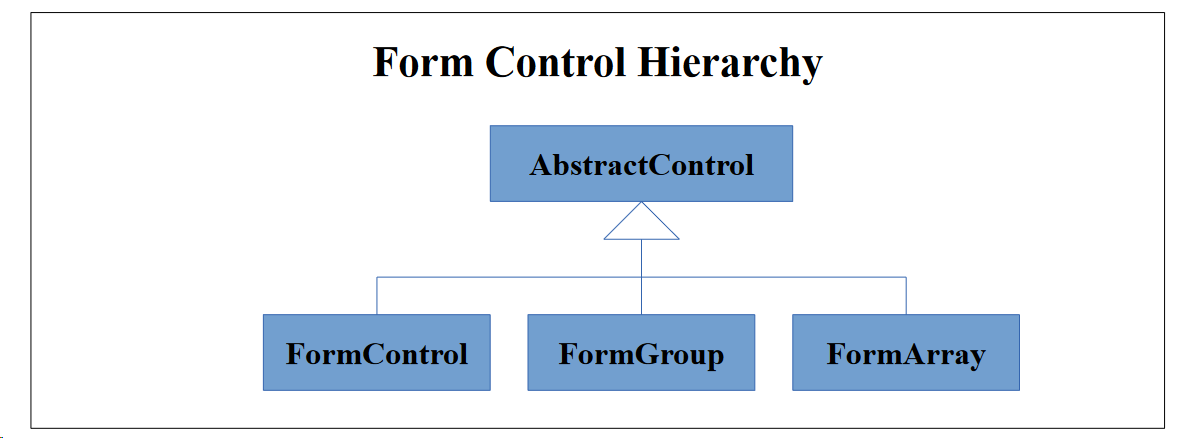
\includegraphics[width=0.75\linewidth]{15_the_forms_package/form_control_hierarchy}
  \label{fig:form_control_hierarchy}
\end{figure}

% The status of a form control is one of:

表单控件的状态是以下之一:

\input{../output/15_the_forms_package/code/15_3_0_6.tex}

% The
% \texttt{AbstractControl}
% class defines a constructor, that takes in validator and async
% validator functions. This class also defines a bunch of getters which map to private
% fields. The value field refers to data we wish to strore within the control:

\texttt{AbstractControl} 类构造器接收一个 validator 和 async validator 函数。
还定义了一系列的 getters 用于映射私有字段。
value 字段代表我们想要存储在表单控件内的数据:

\input{../output/15_the_forms_package/code/15_3_0_7.tex}

% The
% \texttt{\_status}
% field refers to the validator checking:

\texttt{\_status} 字段表示 validator 状态:

\input{../output/15_the_forms_package/code/15_3_0_8.tex}

% The
% \texttt{\_error}
% field returns a map of errors (if any):

\texttt{\_error} 字段返回错误映射(如果有):

\input{../output/15_the_forms_package/code/15_3_0_9.tex}

% The
% \texttt{\_pristine}
% field refers to whether the control’s data has been changed –
% \texttt{pristine()}
% is true if unchanged, and
% \texttt{dirty()}
% is true if changed:

\texttt{\_pristine} 字段代表控件数据是否改变了 —— \texttt{pristine()} 为 true 则表示未变化,
\texttt{dirty()} 为 true 则表示变化了:

\input{../output/15_the_forms_package/code/15_3_0_10.tex}

% The
% \texttt{\_touched}
% field refers to whether the user has visited the control (if does not
% mean that the control’s value has been changed):

\texttt{\_touched} 代表控件是否被用户访问(但这并不意味着控件值发生了变化)

\input{../output/15_the_forms_package/code/15_3_0_11.tex}

% There are also two
% \texttt{xxChanges()}
% getters, for value changes and status changes, that
% return observables:

还有两个 \texttt{xxChanges()} getter,value changes 和 status changes,
返回 observables:

\input{../output/15_the_forms_package/code/15_3_0_12.tex}

% These are initialized to event emitters via:

通过 event emitters 进行初始化:

\input{../output/15_the_forms_package/code/15_3_0_13.tex}

% \texttt{AbstractControl}
% also declares a function:

\texttt{AbstractControl} 还声明了一个函数:

\input{../output/15_the_forms_package/code/15_3_0_14.tex}

% which executes the condition function over the control and its children and return a
% boolean. This
% \texttt{\_anyControls}
% function is used in many helper methods to determine
% information about the control, e.g.:

它对控件及其子控件执行条件函数并返回一个布尔值。
\texttt{\_anyControls} 函数在许多辅助函数中用于确定有关控件的信息,例如:

\input{../output/15_the_forms_package/code/15_3_0_15.tex}

% It has a parent field:

它有一个 parent 字段:

\input{../output/15_the_forms_package/code/15_3_0_16.tex}

% which is used when the state of the control is being updated.

当控件的状态正在更新时使用。

\input{../output/15_the_forms_package/code/15_3_0_17.tex}

% It is set via:

它通过以下方式设置:

\input{../output/15_the_forms_package/code/15_3_0_18.tex}

% Its is hierarchical and this is supplied to find the root:

它是继承的,用于查找根:

\input{../output/15_the_forms_package/code/15_3_0_19.tex}

% The FormControl class is supplied for atomic controls (that do not contain any child
% controls).

FormControl 类是为原子控件(不包含任何子控件)提供的。

\input{../output/15_the_forms_package/code/15_3_0_20.tex}

% Its
% \texttt{\_value}
% field is set via
% \texttt{setValue()}
% method which reacts depending on the four
% optional booleans supplied:

它的 \texttt{\_value} 字段是通过 \texttt{setValue()} 方法设置的,
该方法根据给定的四个可选布尔值做出相应改动:

\input{../output/15_the_forms_package/code/15_3_0_21.tex}

% It has a
% \texttt{reset()}
% method to reset control data:

\texttt{reset()} 方法用于重置控件数据:

\input{../output/15_the_forms_package/code/15_3_0_22.tex}

% The FormGroup class extends AbstractControl:

FormGroup 类继承自 AbstractControl:

\input{../output/15_the_forms_package/code/15_3_0_23.tex}

% Its constructor’s first parameter defines a controls associative map (in constrast to
% FormArray):

它的构造函数的第一个参数定义了一个控件关联映射(与 FormArray 形成对比):

\input{../output/15_the_forms_package/code/15_3_0_24.tex}

% Controls can be registered with FormGroup via:

可以通过以下方式向 FormGroup 注册控件:

\input{../output/15_the_forms_package/code/15_3_0_25.tex}

% The values of all controls in the group may be set via:

group 中所有控件的值可以通过以下方式设置:

\input{../output/15_the_forms_package/code/15_3_0_26.tex}

% Note it throws an exception is any of the controls are missing
% 1
% .

请注意,如果缺少任何控件,它会引发异常 \step{1}。

% The FormArray class extends AbstractControl:

FormArray 类继承自 AbstractControl:

\input{../output/15_the_forms_package/code/15_3_0_27.tex}

% Its constructor’s first parameter is simply an array:

它的构造函数的第一个参数只是一个数组:

\input{../output/15_the_forms_package/code/15_3_0_28.tex}

% It allows you to insert at the end of the array or at a given location, and to remove:

允许你在数组的末尾或给定位置进行插入,删除:

\input{../output/15_the_forms_package/code/15_3_0_29.tex}



\backmatter
\printindex
\end{document}
